\documentclass[10.5pt,a4paper]{article}
\usepackage[a4paper,margin=22mm]{geometry}
\usepackage{amsmath,amssymb,amsthm,mathtools}
\usepackage{fontspec}
\usepackage{xetexko}
\setmainhangulfont{NanumMyeongjo}
\setsanshangulfont{NanumGothic}
\setmonohangulfont{NanumGothicCoding}
\usepackage{booktabs,longtable,array,graphicx,enumitem,xcolor,float}
\usepackage[colorlinks=true,linkcolor=blue!50!black,urlcolor=blue!50!black,citecolor=blue!50!black]{hyperref}
\setlist{itemsep=1pt,topsep=3pt}
\linespread{1.12}
\setlength{\parskip}{3pt}
\setlength{\parindent}{0pt}

\theoremstyle{plain}
\newtheorem{theorem}{정리}[section]
\newtheorem{proposition}[theorem]{명제}
\newtheorem{lemma}[theorem]{보조정리}
\newtheorem{corollary}[theorem]{따름정리}
\newtheorem{conjecture}[theorem]{추측}
\theoremstyle{definition}
\newtheorem{definition}[theorem]{정의}
\newtheorem{example}[theorem]{예}
\newtheorem{observation}[theorem]{수치관찰}
\newtheorem{heuristic}[theorem]{휴리스틱}
\theoremstyle{remark}
\newtheorem{remark}[theorem]{주의}


\usepackage{newunicodechar}
\newunicodechar{≈}{\ensuremath{\approx}}
\newunicodechar{⇒}{\ensuremath{\Rightarrow}}
\newunicodechar{→}{\ensuremath{\to}}
\newunicodechar{↔}{\ensuremath{\leftrightarrow}}
\newunicodechar{≤}{\ensuremath{\le}}
\newunicodechar{≥}{\ensuremath{\ge}}
\newunicodechar{×}{\ensuremath{\times}}
\newunicodechar{∈}{\ensuremath{\in}}
\newunicodechar{⊂}{\ensuremath{\subset}}
\newunicodechar{≠}{\ensuremath{\ne}}
\newunicodechar{∞}{\ensuremath{\infty}}
\newunicodechar{√}{\ensuremath{\surd}}
\newunicodechar{≪}{\ensuremath{\ll}}
\newunicodechar{≫}{\ensuremath{\gg}}
\newunicodechar{∼}{\ensuremath{\sim}}
\newunicodechar{⊕}{\ensuremath{\oplus}}
\newunicodechar{⊗}{\ensuremath{\otimes}}
\newunicodechar{∅}{\ensuremath{\emptyset}}
\newunicodechar{∩}{\ensuremath{\cap}}
\newunicodechar{∪}{\ensuremath{\cup}}
\newunicodechar{±}{\ensuremath{\pm}}
\providecommand{\tightlist}{\setlength{\itemsep}{0pt}\setlength{\parskip}{0pt}}
\usepackage{calc}
\usepackage{url}
\usepackage{fvextra}
\AtBeginDocument{\renewcommand{\figurename}{그림}\renewcommand{\contentsname}{차례}\renewcommand{\abstractname}{초록}}
\newfontfamily\notesfont{DejaVu Sans Mono}[Scale=0.82]

\newcommand{\R}{\mathbb{R}}
\newcommand{\Z}{\mathbb{Z}}
\newcommand{\Q}{\mathbb{Q}}
\newcommand{\C}{\mathbb{C}}
\newcommand{\HH}{\mathbb{H}}
\newcommand{\E}{\mathbb{E}}
\renewcommand{\P}{\mathbb{P}}
\newcommand{\Sym}{\mathrm{Sym}}
\newcommand{\Tr}{\mathrm{Tr}}
\newcommand{\Vol}{\mathrm{Vol}}
\newcommand{\covol}{\mathrm{covol}}
\newcommand{\rd}{\mathrm{rd}}
\newcommand{\Herm}{\mathrm{Herm}}
\newcommand{\tagP}{\textcolor{green!45!black}{\textbf{[증명됨]}}}
\newcommand{\tagPC}{\textcolor{green!45!black}{\textbf{[증명됨(계산기)]}}}
\newcommand{\tagC}{\textcolor{orange!80!black}{\textbf{[조건부]}}}
\newcommand{\tagJ}{\textcolor{purple}{\textbf{[추측]}}}
\newcommand{\tagN}{\textcolor{blue!70!black}{\textbf{[수치관찰]}}}
\newcommand{\tagH}{\textcolor{gray!70!black}{\textbf{[휴리스틱]}}}
\newcommand{\tagL}{\textcolor{teal!70!black}{\textbf{[문헌]}}}
\newcommand{\tagF}{\textcolor{red!70!black}{\textbf{[실패/반증]}}}
\newcommand{\tagM}{\textcolor{green!45!black}{\textbf{[모형에서 증명]}}}
\newcommand{\tagPL}{\textcolor{green!45!black}{\textbf{[증명됨·인용 정리 전제]}}}
\providecommand{\Hom}{\operatorname{Hom}}

\hypersetup{pdftitle={Lattice sphere packing lower bounds beyond c n^2 log log n 2^{-n}: research session report},pdfauthor={Autonomous research loop}}
\title{\textbf{고차원 격자 구 채우기 하한 $c\,n^2\log\log n\cdot2^{-n}$ 을 넘어서려는 시도}\\[4pt]\large 5시간 자율 연구 세션 보고서: 증명된 것, 조건부 결과, 추측, 수치 관찰, 그리고 실패한 접근}
\author{자율 연구 루프 (다중 에이전트 증명·계산·반박 검증)}
\date{2026년 11월 25일 (UTC 06:24 시작, 10:39 기록 종료; 경과 255분)}
\begin{document}
\maketitle
\begin{abstract}
\noindent Klartag (2025) 의 격자 구 채우기 하한 $\delta_n\ge c\,n^2\,2^{-n}$ 과 그 후속 결과 $c\,n^2\log\log n\cdot 2^{-n}$ (Abuya--Gargava--Zhao, Gargava--Gr\"obner--Simkin, 2026) 의 개선을 목표로, ``과제 선택 $\to$ 증명 시도 $\to$ 반례·수치 검증 $\to$ 기록'' 의 절차를 20개 회차(0--19회차) 반복했다. \textbf{차수 $n^2\log\log n$ 을 개선하는 정리는 얻지 못했다.} 얻은 것은 다음과 같다.
(1) 알려진 대칭 논증(Venkatesh, AGZ; GGS 의 순환군 판)의 이득을 하나의 지표 $g=|G|/(2\dim_\Q A)$ 로 기술하고, $\Q$-기약 가군 위의 고정점 없는 작용에서는 이 지표가 $O(\log\log|G|)$ 임을 증명했다(방법의 회계량에 대한 정리이며, 모든 논증에 대한 장벽 정리는 아니다).
(2) Hurwitz/icosian 가군 격자에 대해 명시적 상수의 Klartag 형 한계 $V_n\ge(\tfrac{3}{2e}-o(1))n^2$ ($4\mid n$), $(\tfrac{15}{4e}-o(1))n^2$ ($8\mid n$) 의 증명을 썼고 AI 심사 에이전트 둘이 오류를 찾지 못했다. 단 Gargava (2021) 의 평균값 정리를 전제하며(그 증명은 17회차에서 원문으로 점검했고, icosian 의 경우에는 한 단계의 보수가 필요했다; 그 정리가 기대는 Weil 의 환원 이론은 확인하지 못했다), 문헌 점검에서 선행 결과를 찾지 못했으나 새로움을 단정하지는 않는다; 차수는 $n^2$ 그대로여서 점근적으로는 $c\,n^2\log\log n$ 보다 약하고, 개선은 명시적 선행 상수(Rezvyakova 의 $\tfrac1{2e}$ 대비 3배·7.5배)에 한정된다.
(3) 고정점이 있는(비자유) 작용에 대한 틀 정리 --- 고정된 격자 $\Lambda_W$ 가 class number 1 의 order 위에서 ``경계 안정'' 이면 텐서족 $\Lambda_W\otimes_{\mathcal O}L$ 에서 $V_n\ge(1-o(1))\tfrac{|G|}{4e\dim_\Q A}n^2$ --- 를 증명하고, Leech 격자의 $SL_2(13)$ 대칭에 적용해 $V_n\ge(\tfrac{91}{12e}-o(1))n^2\approx2.79\,n^2$ ($24\mid n$)을 얻었다(Rezvyakova 상수의 15.2배). 이를 위해 나눗셈대수 order 위 가군 격자의 $j$-틀 평균값 공식을 Gargava 의 정리로부터 유도했다. 마지막 회차에서는 class number 가정을 없앤 판(극대 order; AI 심사 2회 통과; 사람의 검증 없음)도 썼는데, 이 판은 14회차 증명의 해석적 부분(19회차 심사자들이 다시 검증하지 않음)과 같은 인용 입력을 물려받으며, 이에 따르면 $SL_2(p)$ 족에서 고정된 $p$ 에 대해 남는 가정은 ``경계 안정'' 과 order 의 극대성(이전 회차의 보고에 의존, 미재확인)이다. AI 심사 에이전트들이 오류를 찾지 못했으나, 인용한 정리들(특히 Gargava 의 정리 16 을 모든 랭크 $\ge2$ 에서 --- Leech 의 경우인 $\Delta_\R=\HH^2$ 에서는 그 인쇄된 증명의 한 단계가 성립하지 않아 17회차에서 원문을 읽고 보수했으며, 그 정리가 기대는 Weil 의 환원 이론은 확인하지 못했다)과 5회차의 계산기 보조 사실에 의존하고, 순수 점근 진술이며(증명 그대로는 $n\gtrsim10^{14}$ 에서야 비자명), 차수는 역시 $n^2$ 이다.
(4) 조사한 군들 가운데 유도한 필요조건을 모두 통과한 것은 $SL_2(p)$ Weil 격자의 텐서족뿐이었다(분류 정리가 아니라 조사 수준의 배제). $p=13$ (Leech 격자)에서는 낮은 랭크 항의 판정량이 정확히 경계($R_U\le1$, 등호가 1638개 직선에서 성립)임을 계산기 보조로 증명했고, 일반 $p$ 의 직선 수준 필요조건을 표수 $p$ 의 곡선 $y^2=x^p-x$ 의 Mordell--Weil 격자에 대한 산술 조건으로 바꿔 썼으며, 직접 계산으로 $p=37$ (72차원)은 불안정임을 정수 인증서로 확인하고, $p=61$ (120차원)은 수행한 모든 구조적 시험에서 위반이 없음을 확인했다(안정성의 증명은 아니다). 또 토러스 부분군의 고정 부분격자가 몫곡선 $Y^2=X^{N+1}-X$ 의 같은 유형의 격자와 정확히 일치함을 보였다(AI 심사 1회; Weil 격자와의 동일시는 Mordell--Weil 사전의 증명 스케치에 의존한다). 이는 $p\le757$ 의 계산에서 고정 부분격자가 왜 짝 unimodular 격자($E_8$, Niemeier, Leech)의 상수배인지를 설명하고 $p=37$ 의 실패를 몫곡선의 조건($s'^2\le p-36$)으로 옮기지만, 어느 격자가 나타나는지와 위반 벡터의 존재 자체는 수치 결과일 뿐이다.
(5) Klartag 과정의 Poisson/퍼셉트론 모형에서 상수 손실의 구조와 정확한 법칙 $V_{LP}\sim\chi^2_{2N}$ 을 얻었으나, 실제 랜덤 격자에서는 $n\le28$ 에서 $V_{LP}/N=1.2$--$1.75$ 로 모형값 2 에 못 미친다(차원에 따라 증가 중, 점근 거동은 미결정).
(6) 소차원에서 비대칭·등변 탐색을 구현해, 등변 과정이 $E_8$, $K_{12}$, $BW_{16}$, $\Lambda_{20}$, Leech 격자를 재발견함을 확인했다(모두 이미 알려진 격자이며, 어느 실험에서도 알려진 최선값을 넘는 격자는 나오지 않았다).
모든 주장은 [증명됨]/[증명됨(계산기)]/[증명됨·인용 정리 전제]/[모형에서 증명]/[조건부]/[추측]/[휴리스틱]/[수치관찰]/[실패] 로 구분했다. 여기서 [증명됨] 은 ``AI 하위 에이전트가 쓴 증명을, 반박하도록 지시받은 다른 AI 에이전트가 검토해 오류를 찾지 못했다'' 는 뜻이며 \textbf{사람의 검증은 전혀 거치지 않았다.}
\end{abstract}
\tableofcontents
\newpage
\section{문제, 현황, 그리고 이 보고서의 위치}

\subsection{문제와 표기}
$\R^n$ 의 격자 $L$ (covolume 1)에 대해
\[
V(L):=\Vol\{\text{원점 중심의, $L\setminus\{0\}$ 과 만나지 않는 가장 큰 열린 공}\},\qquad V_n:=\sup_L V(L)
\]
로 두면 격자 구 채우기 밀도는 $\delta(L)=V(L)/2^n$, $\delta_n=V_n/2^n$ 이다. 동치로, 고정된 격자 $L$ 과 양의 정부호 행렬 $A$ 에 대해 타원체 $\mathcal E_A=\{x: Ax\cdot x<1\}$ 가 $L$-free ($\mathcal E_A\cap L=\{0\}$) 이면 $V\ge \Vol(\mathcal E_A)/\covol(L)$ 이다. 이 보고서 전체에서 $N:=n(n+1)/2=\dim\Sym_n$ 이다.

\subsection{알려진 결과 (2026년 11월 기준, 1회차 문헌 조사로 확정)}
\begin{center}
\begin{tabular}{@{}llll@{}}
\toprule
결과 & $V_n$ 에 대한 한계 & 차원 & 방법 \\
\midrule
Minkowski--Hlawka & $\ge 2\zeta(n)$ & 모든 $n$ & 평균(Siegel) \\
Rogers 1947, Ball 1992 & $\ge 2(n-1)\zeta(n)$ & 모든 $n$ & 평균 + successive minima \\
Vance 2011 & $\ge (6/e)\,n$ & $4\mid n$ & Hurwitz 사원수 가군 \\
Venkatesh 2013 & $\ge \tfrac12 n\log\log n$ & 희소 & 원분체 $\Z[\zeta_m]$ 가군, 궤도 크기 $m$ \\
Gargava--Viazovska 2024 & $\ge n\log\log n$ & 희소 & 랜덤 ideal 격자 \\
Campos--Jenssen--Michelen--Sahasrabudhe & $\ge(\tfrac12-o(1))n\log n$ & 모든 $n$ (비격자) & 그래프 이론 \\
\textbf{Klartag 2025} & $\ge c\,n^2$ & 모든 $n$ & 확률적으로 진화하는 타원체 \\
Rezvyakova 2026 & $\ge(\tfrac1{2e}-o(1))\,n^2$ & $n\to\infty$ & Klartag 증명의 상수 추적 \\
Abuya--Gargava--Zhao 2026 & $\ge c\,n^2\log\log n$ & 희소 & Klartag $\times$ 원분 대칭 \\
\textbf{Gargava--Gr\"obner--Simkin 2026} & $\ge c\,n^2\log\log n$ & 모든 큰 $n$ & 원분 접착(gluing) 구성 \\
\midrule
Kabatiansky--Levenshtein 1978 & $\le 2^{0.401n}$ & & 구면 부호 \\
OpenAI ``Ten Advances'' 2026 (Ch.\,1--2) & $\le 2^{(0.3956+o(1))n}$ & & Cohn--Elkies LP 의 정확한 지수 \\
Venkatesh 의 추측 & $\le n^2(\log n)^{O(1)}$ ? & & ``격자의 자유도는 $n^2$'' \\
\bottomrule
\end{tabular}
\end{center}
사용자가 올려 준 두 논문은 위 표의 Klartag 2025(하한)와 OpenAI 2026(상한)이며, ``$\log\log n$ 이 붙은 최신 결과''는 Abuya--Gargava--Zhao (arXiv:2606.05105) 와 그것을 모든 차원으로 확장한 Gargava--Gr\"obner--Simkin (arXiv:2610.12619) 이다.

\subsection{Klartag 방법의 핵심 (이 보고서에서 계속 쓰는 언어)}
격자 $L$ 을 고정하면 $L$-free 행렬 전체
\[
\mathcal R_L=\{A\in\Sym_n:\ Ax\cdot x\ge 1\ \ \forall x\in L\setminus\{0\}\}
\]
는 국소 유한 다면체(\emph{Ryshkov 다면체})이고, 꼭짓점이 Voronoi 의 \emph{perfect form}, $\det$ 의 국소 최소점이 \emph{extreme form} 이다. Klartag 과정은 $\mathcal R_L$ 안에서의 브라운 운동 $dA_t=\pi_t(dW_t)$ 으로, 면에 닿으면(=격자점이 타원체 경계에 닿으면) 그 면에 달라붙고(sticky), 자유도 $N_t=\dim F_t$ 가 0이 되는 꼭짓점에서 멈춘다. $\log\det$ 의 오목성으로
$\ \E\log\det A_T\le n\log a_0-\tfrac12\int_0^T\E[\|A_t\|_{op}^{-2}N_t]\,dt$
이고, 접촉점 수의 기댓값은 반사원리와 Siegel 평균값 공식(1차 모멘트)만으로 $\lesssim e^{n^2t/8}$ 로 제어된다. 요점은 \emph{``자유도 하나가 접촉쌍 하나를 흡수한다''} 는 회계이며, 대칭 격자 버전(AGZ, GGS)은 \emph{``궤도 하나가 자유도 하나만 소모한다''} 로 이 회계를 개선한 것이다:
\[
V\ \gtrsim\ \frac{(\text{궤도 크기 } w)\times(\text{불변 이차형식 공간의 차원 } D)}{2e}.
\]

\subsection{이 연구 세션이 한 일과 하지 못한 일 (정직한 요약)}
\begin{itemize}
\item \textbf{하지 못한 일.} $c\,n^2\log\log n\cdot 2^{-n}$ 의 \emph{차수}를 개선하는 정리는 얻지 못했다. 이는 오래된 미해결 문제이며, 5시간짜리 탐색의 현실적인 목표는 (i) 방법의 한계를 정확히 규명하고 (ii) 검증 가능한 부분 결과와 (iii) 구체적인 다음 공격 지점을 남기는 것이었다.
\item \textbf{한 일.} \S\ref{sec:summary} 의 표에 [증명됨]/[조건부]/[추측]/[수치관찰] 로 구분해 정리했다. 요지는 다음 다섯 가지다.
 \begin{enumerate}
 \item \textbf{(통일과 한계)} 대칭을 이용하는 모든 알려진 논증을 하나의 이득 공식 $g=|G|/(2\dim_\Q A)=\tfrac12\sum_{g\in G}\rho(g)^2$ 로 통일하고, \emph{고정점 없는 작용}으로는 $\log\log$ 를 넘을 수 없음을 증명했다. 비자유 작용에 대해서는 ``텐서 안정성'' 이라는 판정 기준과 여러 no-go 정리를 얻었다 (\S\ref{sec:sym}).
 \item \textbf{(명시적 상수)} Hurwitz/icosian 가군 격자에 대해 Klartag 형 한계 $V_n\ge(\tfrac3{2e}-o(1))n^2$ ($4\mid n$), $(\tfrac{15}{4e}-o(1))n^2$ ($8\mid n$) 를 완전한 증명으로 쓰고 독립 심사를 거쳤다 --- Rezvyakova 상수 $\tfrac1{2e}$ 의 3배, 7.5배. 차수는 $n^2$ 그대로다 (\S\ref{sec:quat}).
 \item \textbf{(유일하게 남은 차수 개선 후보)} 자유 작용의 한계를 피하는 유일한 후보로 $SL_2(p)$ Weil 격자의 텐서족을 찾았고, $p=13$ (Leech 격자)에서 ``정확히 경계 안정'' 임을 계산기 보조 정리로 증명했다. 일반 $p$ 에서의 성립 여부는 Weil 격자(=곡선 $y^2=x^p-x$ 의 Mordell--Weil 격자)의 산술 문제로 환원되며, 성립한다면 $n^{2+c}$ 형의 하한을 주게 되므로(기존 추측과 충돌) 어느 쪽이든 흥미롭다 (\S\ref{sec:leech}).
 \item \textbf{(모형)} Klartag 과정을 랜덤 선형계획(음의 마진 퍼셉트론)으로 재해석하는 Poisson 모형을 세워 상수의 손실($\tfrac1{2e}\to\tfrac12\to1$)을 설명하고, 모형에서의 정확한 법칙 $V_{LP}\sim\chi^2_{2N}$ 을 얻었다. 그러나 실제 랜덤 격자에서는 $n\le28$ 까지 이 예측이 성립하지 않음도 실험으로 확인했다 (\S\ref{sec:perceptron}).
 \item \textbf{(소차원의 직접 구성)} $n\le12$ 의 비대칭 탐색과 $n\le24$ 의 대칭(등변) 탐색을 구현·검증했다. 대칭 과정은 $E_8,K_{12},BW_{16},\Lambda_{20}$, Leech 를 실제로 찾아내며, ``$V\approx$ (궤도 크기/2)$\times$(불변형식 차원)'' 이라는 스케일링 법칙이 관찰된다 (\S\ref{sec:numerics}, \S\ref{sec:equiv}).
 \end{enumerate}
\end{itemize}

\subsection{연구 절차}
요청받은 절차(로그 읽기 $\to$ 과제 선택 $\to$ 증명 시도/반례 탐색/계산 검증 $\to$ 막힌 지점 기록 $\to$ 로그 저장)를 회차 단위로 반복했다. 각 회차는 ``증명/계산 담당'' 하위 에이전트와, 그 결과를 \emph{반박하도록} 지시받은 독립 ``심사'' 에이전트의 쌍으로 구성했고, 심사를 통과하지 못한 주장은 강등하거나 폐기했다. 모든 수치는 실제 실행한 코드에서 나온 것이며 코드와 원자료는 저장소의 \texttt{sphere\_packing\_research/rounds/} 아래에 있다. 회차별 기록은 \texttt{research\_log.md} 에 있다.

\section{결과 요약표}\label{sec:summary}

지위 표기: \tagP\ 완전한 증명(하위 에이전트 작성 + 독립 심사 통과), \tagPL\ 인용한 문헌 정리를 전제로 한 완전한 증명, \tagPC\ 정수 연산에 의한 계산기 보조 증명(독립 재계산 통과), \tagM\ Poisson/가우스 모형 안에서의 증명, \tagC\ 조건부, \tagJ\ 추측, \tagH\ 휴리스틱, \tagN\ 수치 관찰, \tagF\ 실패·반증. ``심사'' 는 해당 주장을 \emph{반박하도록} 지시받은 독립 에이전트의 검토를 뜻하며, 사람에 의한 동료 심사가 아니다 --- 아래의 [증명됨] 은 모두 그 수준의 검증임을 밝혀 둔다.

\begin{center}
\small
\renewcommand{\arraystretch}{1.25}
\begin{longtable}{@{}p{0.6cm}p{11.2cm}p{2.6cm}p{1.2cm}@{}}
\toprule
\# & 진술 & 지위 & 위치\\
\midrule
\endhead
\multicolumn{4}{@{}l}{\textbf{A. 대칭을 이용하는 방법의 통일과 한계}}\\
A1 & 이득 항등식: Klartag 대비 이득 $g=|G|/(2\dim_\Q A)=\tfrac12\sum_{g}\rho(g)^2$; 불변형식 차원 $D\approx k^2\dim_\Q\Delta/2$ & \tagP & \S\ref{sec:sym}\\
A2 & 고정점 없는 작용이면 $g\le 24\,c/\varphi(c)=O(\log\log|G|)$ --- 자유 작용 기반 논증(Venkatesh, AGZ 형)은 $\log\log$ 를 넘지 못한다 & \tagP\ (Zassenhaus 구조정리 인용) & \S\ref{sec:sym}\\
A3 & 비자유 작용의 평균값 공식 $\E\#=cV+\sum_UT_U$, $T_U\approx V^f\mathrm{poly}(n)R_U^{k/2}$; ``텐서 안정성'' $R_U\le1$ 판정 기준 & \tagP\ (스케치 수준; 심사 통과) & \S\ref{sec:sym}\\
A4 & No-go: $\Delta=\Q$ 인 텐서형 격자는 항상 불안정; 소수 위수 원소의 엔트로피 부등식; unimodular 강직성 보조정리($R_U\ge1$, 등호는 $a=b$ 이고 자유일 때뿐) & \tagP & \S\ref{sec:sym}\\
A5 & GGS 원분 접착: $M/C=1/\mu_M(\mathcal N)$; 홀수 $M$ 에서 소인수 $\le3$ 개(또는 4개이고 $\{3,5,7,11\}$ 이 아님)이면 $M/C\le M/\varphi(M)$ & \tagP & \S\ref{sec:gluing}\\
A6 & 약수 24개 이하의 모든 시험 모듈러스에서 $M/C>M/\varphi(M)$ 인 admissible 접착 데이터 없음; 일반적 상계는 미증명 & \tagN, \tagJ & \S\ref{sec:gluing}\\
\midrule
\multicolumn{4}{@{}l}{\textbf{B. 명시적 상수 (차수는 $n^2$)}}\\
B1 & $D_\R\cong\mathbb K^s$ 인 나눗셈대수와 유한군 $G\subset D^\times$: $V_{k\delta}\ge(1-o(1))\tfrac{w}{4e\delta}n^2$ & \tagPL & \S\ref{sec:quat}\\
B2 & Hurwitz: $V_n\ge(\tfrac3{2e}-o(1))n^2$ ($4\mid n$); icosian: $V_n\ge(\tfrac{15}{4e}-o(1))n^2$ ($8\mid n$) & \tagPL & \S\ref{sec:quat}\\
B3 & 행렬 블록이 있는 일반 나눗셈대수로의 확장(개정본 \S7) & \tagC\ (미심사) & 부록 \ref{app:proof}\\
\midrule
\multicolumn{4}{@{}l}{\textbf{C. $SL_2(p)$ Weil 격자 텐서족 (유일하게 남은 차수 개선 후보)}}\\
C1 & Leech 격자는 $\Delta_{13}=\HH\otimes\Q(\sqrt{13})$ 의 극대 order 위의 랭크 3 가군, $\mathrm{Aut}_\Delta=SL_2(13)$; 모든 $\Delta$-직선에서 $R_U\le1$, 등호는 정확히 1638개 직선; 평면은 $R_U\le0.1001$ & \tagPC & \S\ref{sec:leech}\\
C2 & $(p+1)/2$ 가 합성수이면 unimodular Weil 격자는 텐서 불안정($p=17,29,41,\dots$); 소수이면 고정공간은 분리 토러스의 홀수 위수 부분군에서만 나오고 정확히 경계 & \tagP & \S\ref{sec:leech}\\
C3 & Mordell--Weil 재정식화: $W_p$ 는 $\mathrm{Hom}(\mathrm{Jac}(y^2=x^p-x),E)$ 에 뒤틀린 형식을 준 것; 직선 안정성 $\iff N_{F/\Q}(q_F(\phi))\ge((p-1)/4)^2$; 특히 모든 사상 $C_p\to E$ 의 차수 $\ge(p-1)/2$ 필요 & \tagP\ (일부 문헌 미열람) & \S\ref{sec:leech}\\
C3$'$ & \textbf{$p=37$ 은 불안정}: 72차원 짝 unimodular Weil 격자의 $C_3$-고정격자는 $\sqrt3N(D_4^6)$ 이고 그 근에서 $N(\nu)=63<81$, $R_U\ge(9/7)^4$ & \tagPC\ (독립 구현 3개; 정수 인증서) & \S\ref{sec:weilcomp}\\
C3$''$ & $p=61$ (120차원): 모든 부분군류의 isotypic 성분에서 $R_U\le1$ (정수 연산), 랭크 $\le40$ 인 모든 구조적 부분격자에서 위반 벡터 없음; $p=157,277,397$ 의 랭크 8·24 고정 부분격자도 통과. 전체 격자는 미결정 & \tagPC/\tagN & \S\ref{sec:p61}\\
C4 & 수정된 양자택일: 무한히 많은 $p$ 에서 경계 안정 $\Rightarrow$ (텐서족의 등변 Klartag 정리가 $k\ge Cr\log n$ 에서 성립하면) $V_n\gtrsim n^{5/2}/\sqrt{\log n}$; 아니면 Weil 격자에 ``불균형한 짧은 벡터'' 가 존재($p=37$ 처럼). $k\approx r$ 에서는 호흡 모드 때문에 이득 없음 & \tagJ, \tagC & \S\ref{sec:leech}\\
\midrule
\multicolumn{4}{@{}l}{\textbf{D. 모형과 장벽}}\\
D1 & Poisson 모형에서 대각합-LP 최적 타원체의 부피는 정확히 $\chi^2_{2N}$ (평균 $n(n+1)$); 가우스 모형의 임계값 $v^*=(2/e)N$ & \tagM & \S\ref{sec:perceptron}\\
D2 & 격자의 대각합-LP 는 쌍대 형식의 Voronoi 환원(최적점은 perfect form) & \tagP & \S\ref{sec:perceptron}\\
D3 & 실제 랜덤 격자: $V_{LP}/N=1.2$--$1.75$ ($n=14..28$, 증가 중; Poisson 예측 2), $n\le8$ 에서는 root 격자가 지배 & \tagN & \S\ref{sec:perceptron}\\
D4 & $P_V\ge e^{-2n^2\log n-n^2}$ ($V\le V_n/2$); 따라서 Poisson 형 꼬리 $P_V\le e^{-cV}$ 이면 $V_n\le Cn^2\log n$ & \tagP & \S\ref{sec:perceptron}\\
D5 & ``$V_n\asymp n^2\log n$'' (모형의 존재 임계), ``과정 기반 구성은 $\Theta(n^2)$ 을 못 넘는다'' & \tagH\ (심사에서 강등) & \S\ref{sec:perceptron}\\
\midrule
\multicolumn{4}{@{}l}{\textbf{E. 소차원의 직접 실험}}\\
E1 & Klartag 과정을 동결까지: $\E V_{final}/N\in[0.93,1.26]$ ($n=2..10$); $n\le8$ 은 root 격자에 도달, $n\ge9$ 는 미도달 & \tagN & \S\ref{sec:numerics}\\
E2 & 등변 과정: $E_8$, $K_{12}$, $BW_{16}$, $\Lambda_{20}$, Leech 도달; $V_{perf}\approx1.06\,(wD/2)$ & \tagN & \S\ref{sec:equiv}\\
E3 & 알려진 최선 격자를 넘는 $V$ 는 어느 실험에서도 나오지 않음 & \tagN & \\
\bottomrule
\end{longtable}
\end{center}

\section{작은 차원에서의 직접 실험 ($n\le10$)}\label{sec:numerics}

사용자의 제안(``작은 $n$ 에서 기존 구성들을 직접 해 보고 규칙성을 찾자'')에 따라 2회차에서 두 가지를 구현했다. 모든 결과는 별도의 검증 에이전트가 처음부터 다시 짠 열거 코드로 재확인했다(저장된 최종 형식 $1878+3403$ 개 전부 $L$-free 이고 perfect; 알려진 최적값을 넘는 $V$ 는 없음).

\subsection{Klartag 과정을 동결될 때까지 실행}
격자는 Goldstein--Mayer 족($\{x\in\Z^n:x_n\equiv a\cdot x'\bmod p\}$, $p=100003$)과 $\Z^n$; $dA=\pi_F(dW)$ 를 Euler 스텝으로 이산화하되 각 선분 위에서 접촉 시각을 정확히 계산했다.

\begin{center}
\begin{tabular}{@{}rrrrrrrr@{}}
\toprule
$n$ & 실행 수 & $\E V_{final}$ & $\E V_{final}/N$ & $\E V_{final}/n^2$ & 최선 $V_n$ & 평균/최선 & 최밀 격자 도달 비율\\
\midrule
2 & 207 & 3.628 & 1.21 & 0.907 & 3.628 & 1.000 & 1.000\\
3 & 225 & 5.924 & 0.99 & 0.658 & 5.924 & 1.000 & 1.000\\
4 & 220 & 9.316 & 0.93 & 0.582 & 9.870 & 0.944 & 0.468 ($D_4$)\\
5 & 290 & 14.48 & 0.97 & 0.579 & 14.89 & 0.973 & 0.845 ($D_5$)\\
6 & 223 & 22.67 & 1.08 & 0.630 & 23.87 & 0.950 & 0.673 ($E_6$)\\
7 & 112 & 35.20 & 1.26 & 0.718 & 37.80 & 0.931 & 0.786 ($E_7$)\\
8 & 163 & 44.79 & 1.24 & 0.700 & 64.94 & 0.690 & 0.331 ($E_8$)\\
9 & 100 & 45.27 & 1.01 & 0.559 & 74.64 & 0.607 & 0.000\\
10 & 50 & 56.81 & 1.03 & 0.568 & 94.23 & 0.603 & 0.000\\
\bottomrule
\end{tabular}
\end{center}

\begin{observation}\tagN
\begin{enumerate}
\item \textbf{$V_{final}\approx N=n(n+1)/2$.} 경로 전체에서 $V(t)/k(t)\approx1$ ($k$ = 독립 접촉쌍의 수; $k\ge36$ 에서 $0.96$--$1.02$). 즉 ``쓸어 담은 부피 $\approx$ 접촉쌍 수'' 가 상수 $\approx1$ 로 성립하고, 과정을 끝까지 돌리면 상수는 $c\approx\tfrac12$ 근처다 (증명된 값 $\tfrac1{2e}$).
\item \textbf{$n\le8$ 과 $n\ge9$ 는 다른 체제.} $n\le8$ 에서는 과정이 높은 확률로 root 격자($D_4,D_5,E_6,E_7,E_8$)에서 끝나지만, $n=9,10$ 에서는 한 번도 최밀 격자에 도달하지 못하고 $n^2$ 법칙으로 내려앉는다.
\item 동결된 형식은 작은 차원에서 단순 꼭짓점이 아니다: 최종 접촉쌍 수의 평균은 $n=4..10$ 에서 $10.9,19.2,33.6,56.8,71.4,60.6,76.1$ ($N=10,15,21,28,36,45,55$). (따라서 Poisson 모형의 ``일반 위치'' 가정은 작은 $n$ 의 실제 격자에서는 성립하지 않는다.)
\item 동결 시간은 Klartag 의 $T=16\log n/n^2$ 규모(중앙값/$T$ = $1.1$--$1.4$, $n=6..10$)이고 $V(T)$ 가 최종 부피의 $82$--$95\%$.
\end{enumerate}
\end{observation}

\subsection{Voronoi 형 국소 탐색 (sticky walk + 탐욕 LP 하강)}
$\Z^n$ 위의 형식에서 무작위 방향으로 면을 따라 perfect form 까지 걷고, 이어서 $\min\Tr(A^{-1}B)$ LP 로 꼭짓점에서 꼭짓점으로 내려가 extreme form (perfect + eutactic)에 도달한다.
\begin{observation}\tagN
\begin{enumerate}
\item 전형적 extreme form 의 중앙값: $V\approx(0.63\text{--}0.70)\,n^2$ ($n=9,10$). 최선 격자는 그보다 $1.4$--$1.8$ 배.
\item 접촉쌍 수와 $V$ 의 순위상관은 $0.88$--$0.95$; extreme form 의 평균 접촉쌍 $\approx2N$, 최선 격자는 $3.0$--$3.3N$ ($E_8$: $120=3.33N$).
\item \textbf{유리 구조.} 발견된 모든 extreme form 은 작은 분모의 유리 형식이다: $qA$ 가 정수이고 $q\in\{2,4,6,8,10,12,14\}$; $q=2$ 는 정확히 root 격자들, 대다수는 $q=4$ (최소노름 4인 정수 격자, 최소벡터 사이 내적 $\in\{0,\pm1,\pm2\}$).
\item $\Lambda_9$ ($136$쌍), $\Lambda_{10}$ ($168$쌍), $K_{10}$ 이 정확한 행렬식과 키싱 수로 재현된다; $n=9$ 에서 $\Lambda_9$ 도달 비율은 perfect 단계 $1.5\%$, 탐욕 하강 후 $23\%$.
\end{enumerate}
\end{observation}

\subsection{소차원 데이터가 말해 주는 것과 말해 주지 않는 것}
알려진 최밀 격자의 $V_n/n^2$ 는 $n\le11$ 에서 $0.6$--$1.0$, $n=16$ 에서 $3.8$, $n=24$ 에서 $56$, $n=48$ 에서 $2832$ 로, 접근 가능한 모든 차원에서 $n^2$ 규모보다 지수적으로 크다. 물리 문헌의 수치(Kallus--Marcotte--Torquato: 순차 LP 로 얻은 isostatic extreme 격자의 전형적 값 $V\approx0.0567\,d^{3.01}$, $d=15..24$; Andreanov--Scardicchio: 랜덤 perfect 격자 $V/d^2\in[0.65,0.94]$, $d=8..19$)도 이 범위에서는 다항식과 지수 성장을 구분하지 못한다. 결론적으로 \emph{소차원의 규칙성(root 격자, laminated 격자, 큰 키싱 수)은 점근 영역 $V\sim n^2$ 과는 다른 체제에 속하며}, 점근 문제에 쓸 수 있는 구조적 교훈은 다음 둘이다: (i) 접촉쌍 수와 부피 사이의 회계 $V\approx(\text{상수})\times(\text{독립 접촉쌍 수})$, (ii) 좋은 격자는 종속적인 접촉(대칭 궤도)을 대량으로 갖는다 --- 이것이 \S\ref{sec:sym} 의 대칭 이론으로 이어진다.

\section{등변 Klartag/Voronoi 탐색: 대칭 과정은 실제로 어떤 격자를 찾는가 (8회차)}\label{sec:equiv}

사용자의 제안(``작은 $n$ 에서 실례를 직접 구성해 규칙성을 보자'')을 대칭 격자족에 적용했다. 고정된 가군 $\mathcal O^k$ ($\mathcal O$: Eisenstein, Gauss, Hurwitz 정수환, $\Z[\zeta_m]$, icosian 환) 위에서, $G$-불변 형식 공간 $\mathcal Q$ (차원 $D$) 안의 이산 Klartag 과정(자유 부분공간의 무작위 방향, 정확한 직선 탐색, 접촉 유지)을 $\mathcal Q$-perfect 형식까지 돌리고, 이어서 탐욕 LP 하강으로 $\mathcal Q$-extreme 형식에 도달한다. 총 1152회 실행(프로그램 충돌 0; 그중 7회는 탐욕 하강 단계의 알려진 버그의 영향을 받았다 --- 검증 보고 참조). 실행 수는 족마다 크게 다르다: $n\le16$ 은 수십~수백 회, $n\ge20$ 은 소수(Hurwitz $k=5$: 10회, icosian $k=3$: 24회, $\Z[\zeta_{13}]$: 3회, Hurwitz $k=6$: 2회). 독립 검증 에이전트가 모든 최종 형식을 정수 연산으로 재검증했고(격자점 없음, 최소벡터 수, 행렬식), 알려진 최선값을 넘는 $V$ 는 없었다($\max V/V_{best}=1.000000$).

\begin{center}
\small
\begin{tabular}{@{}llrrrrll@{}}
\toprule
족 & $k$ & $n$ & $w$ & $D$ & $wD/2$ & 첫 perfect 형식의 $V$ 중앙값 & 도달한 기록 격자 (빈도)\\
\midrule
Eisenstein & 4 & 8 & 6 & 16 & 48 & 64.9 & $E_8$ (80--93\%)\\
Hurwitz & 2 & 8 & 24 & 6 & 72 & 64.9 & $E_8$ (100\%)\\
icosian & 1 & 8 & 120 & 2 & 120 & 64.9 & $E_8$ (100\%)\\
$\Z[\zeta_7]$ & 2 & 12 & 14 & 12 & 84 & 133.4 & $K_{12}$ (33\%)\\
Hurwitz & 3 & 12 & 24 & 15 & 180 & 170.9 & --- ($\Lambda_{12}$ 밀도의 형식; $K_{12}$ 0/80)\\
Hurwitz & 4 & 16 & 24 & 28 & 336 & 335 & $BW_{16}$ (12--40\%)\\
icosian & 2 & 16 & 120 & 12 & 720 & 632 & $BW_{16}$ (42--67\%)\\
Hurwitz & 5 & 20 & 24 & 45 & 540 & 534 & $\Lambda_{20}$ (2/10, LP 하강 후)\\
$\Z[\zeta_{13}]$ & 2 & 24 & 26 & 24 & 312 & 361 & --- (최대 834)\\
Hurwitz & 6 & 24 & 24 & 66 & 792 & 922 & --- (최대 1573)\\
\textbf{icosian} & \textbf{3} & \textbf{24} & 120 & \textbf{30} & 1800 & 1840 & \textbf{Leech (11/24)}\\
\bottomrule
\end{tabular}
\end{center}

\begin{observation}\tagN\ (검증자가 전 항목 재현)
\begin{enumerate}
\item \textbf{대칭 과정은 기록 격자를 그대로 찾는다.} 특히 icosian 랭크 3 가군에서는 자유도가 $D=30$ 개뿐인 탐색이 24차원 Leech 격자($V=32372.9$, 최소벡터 196560개; 짝 unimodular·최소노름 4 임을 정수 연산으로 확인)에 절반 가까운 빈도로 도달한다. 공정한 비교를 위해 적어 두면, 비대칭 Klartag 과정(2회차)은 $n=9,10$ 에서 최밀 격자에 한 번도 도달하지 못했지만 비대칭 Voronoi 탐색에 같은 탐욕 하강을 붙이면 $\Lambda_9$ 에 $23\%$, $\Lambda_{10}$ 에 $4.5$--$14\%$ 도달했다. 대칭이 항상 유리한 것도 아니다(Eisenstein $k=5$, $n=10$ 은 비대칭 탐색보다 낫지 않았다).
\item \textbf{스케일링 법칙 $V_{perf}\approx1.06\cdot wD/2$.} 첫 $\mathcal Q$-perfect 형식의 부피 중앙값을 $wD/2$ 로 나눈 값은 $n\ge10$ 인 17개 (족,$k$) 점에서 $[0.88,1.59]$, 기하평균 $1.06$, 로그--로그 기울기 $0.94$ ($wD/2=50..1800$). 즉 비대칭의 ``$V\approx N$'' 이 ``$V\approx\tfrac w2\times D$'' (접촉 궤도 하나가 자유도 하나) 로 일반화되며, 이는 정리 \ref{thm:quatC} 의 $wD_k/(2e)$ 와 같은 구조다.
\item 각 차원에서 족의 순위는 $wD/2$ 순이다 ($n=24$: icosian $>$ Hurwitz $>\Z[\zeta_{13}]$).
\item 발견된 모든 $\mathcal Q$-perfect 형식은 유리 형식이고(기초적 증명), 기록 격자들의 분모는 $q=2$ (root 격자) 또는 $q=4$ ($\Lambda_{10},K_{12},BW_{16},\Lambda_{20}$, Leech).
\item 기록 격자들은 극도로 퇴화된 꼭짓점이다(Leech: 접촉 궤도 1638개 대 $D=30$). 반면 가장 큰 사례의 ``일반적'' 동결 형식은 단순 꼭짓점이다(Hurwitz $k=6$: 정확히 $D=66$ 궤도).
\end{enumerate}
\end{observation}
\paragraph{해석 \tagH.} 소차원의 ``좋은 실례'' 는 대칭이 큰 족 안에서 찾으면 실제로 구성적으로 나온다 --- 그러나 그것들은 $V\gg wD$ 인 예외적 꼭짓점이다. 첫 $\mathcal Q$-perfect 형식의 부피는 $V\approx wD/2$ 규모이고, 기록 격자는 주로 그 뒤의 탐욕 LP 하강에서 나온다($n=24$ icosian 에서는 24회 중 11회가 Leech 에서 끝나므로, 이 크기에서는 ``전형적 종착점'' 이 아직 예외적 격자다). 차원이 커지면 종착점이 $V\approx wD/2$ 규모로 내려앉으리라는 것은 정리 \ref{thm:quatC} 와 $n\le24$ 의 추세에 근거한 추정이다. 따라서 점근 문제에서 대칭으로 얻을 수 있는 것은 이득 인자 $g=wD/n^2\approx|G|/(2\dim_\Q A)$ 이고, 이것이 얼마나 클 수 있는가가 \S\ref{sec:sym} 의 주제다. 최선 형식들의 정수 Gram 행렬은 \texttt{rounds/R8\_equivariant/best\_forms.json} 에 있다.

\section{대칭 격자족: 이득 공식, 자유 작용의 한계, 비자유 작용}\label{sec:sym}

이 절은 3회차·5회차·7회차의 결과이다. 목표는 ``Klartag$\times$대칭'' 논증(AGZ, GGS)이 원리적으로 어디까지 갈 수 있는지를 군론·격자론의 언어로 정확히 서술하는 것이다.

\subsection{설정과 이득 항등식}
$G$ 를 유한군, $W$ 를 $\Q$-기약 $G$-가군, $A\subset\mathrm{End}_\Q(W)$ 를 $G$ 의 $\Q$-선형 생성(단순 대수), $\Delta=\mathrm{End}_G(W)$ (나눗셈대수)라 하자. 그러면 $A\cong M_r(\Delta^{op})$, $W\cong\Delta^r$, $\dim_\Q A=r^2\dim_\Q\Delta$, $\dim_\Q W=r\dim_\Q\Delta$ 이다. $G$ 가 $W^k$ ($n=k\dim_\Q W$)에 대각으로 작용할 때, $G$-불변 격자들은 $\Lambda=(W_\Z)^k\gamma$, $\gamma\in GL_k(\Delta_\R)$ 꼴의 족을 이루고 ($W_\Z\subset W$ 는 $G$-불변 격자, $\Delta_\R=\Delta\otimes\R$), $G$-불변 이차형식의 공간은 $\Delta_\R$ 위의 Hermite $k\times k$ 행렬 공간과 같다.

\begin{proposition}[이득 항등식]\label{prop:gain}\tagP\ (항등식) / \tagH\ (``이득'' 으로의 해석: 정리로 실현된 것은 자유 작용·$D_\R=\mathbb K^s$ 인 경우뿐, \S\ref{sec:quat})\
$\rho:=\chi_W/\chi_W(1)$ 이라 하면
\[
\sum_{g\in G}\rho(g)^2=\frac{|G|}{\dim_\Q A},\qquad
D_k:=\dim(\Sym^2 (W^k)_\R)^G=\frac1{|G|}\sum_{g}\frac{\chi(g)^2+\chi(g^2)}2=\frac{k^2\dim_\Q\Delta}{2}+O(k)\quad(\chi=k\chi_W).
\]
따라서 일반 궤도의 크기가 $w=|G|$ 이고 $-1\in G$ 일 때, 등변 Klartag 논증의 휴리스틱 부피 $wD_k/(2e)$ 의 Klartag ($w=2$, $D=N$) 대비 \emph{이득}은
\[
g(G,W)\;=\;\lim_{k\to\infty}\frac{wD_k}{2N}\;=\;\frac{|G|}{2\dim_\Q A}\;=\;\frac12\sum_{g\in G}\rho(g)^2 .
\]
\end{proposition}
\begin{proof}
$\chi_W$ 는 유리수 값이므로 $\sum_g\chi_W(g)^2=|G|\langle\chi_W,\chi_W\rangle=|G|\dim_\Q\mathrm{End}_G(W)=|G|\dim_\Q\Delta$. 이중 중심화 정리로 $\dim A\cdot\dim\Delta=(\dim W)^2$ 이므로 첫 식이 나온다. 둘째 식은 $\Sym^2$ 의 지표 공식이고, $\frac1{2|G|}\sum_g\chi(g)^2=k^2\dim\Delta/2$, 나머지 항은 $O(k)$ 이다. $N\sim k^2(\dim W)^2/2$ 를 대입하면 $wD_k/(2N)\to|G|\dim\Delta/(2(\dim W)^2)=|G|/(2\dim A)$.
\end{proof}
예: $\mu_m$ on $\Q(\zeta_m)$ ($m$ 짝수): $g=m/(2\varphi(m))$ (AGZ/GGS 의 $\log\log$). Hurwitz 단위군 $2T$ ($|G|=24$, $\dim A=4$): $g=3$. Icosian 단위군 $2I=SL_2(5)$ ($120$, $8$): $g=7.5$. $W$ 가 $\mathrm{Ind}_{\{\pm1\}}^G(\mathrm{sgn})$ 의 배수이면($-1$ 을 법으로 한 정칙표현; $\rho(\pm1)=\pm1$, 그 밖에서 0) $\tfrac12\sum\rho^2=1$: 이득 없음(기약이 아닌 경우로의 형식적 확장).

\subsection{고정점 없는 작용으로는 $\log\log$ 를 넘을 수 없다}
\begin{theorem}[자유 작용의 한계]\label{thm:fpf}\tagP\ (구조정리는 인용)\
$G$ 의 단위원 아닌 어떤 원소도 $W$ 에서 고윳값 1을 갖지 않는다고 하자. 그러면
\[
\sum_{g\in G}\rho(g)^2=\sum_{\substack{C\le G\ \text{순환}\\ |C|\ \text{제곱인수 없음}}}\frac1{\varphi(|C|)}\ \le\ 240\prod_{\ell\,\mid\,|G|}\frac \ell{\ell-1}\ =\ O(\log\log|G|)\qquad(\ell\text{ 는 소수}).
\]
즉 이득 지표는 $g\le120\prod_\ell\tfrac\ell{\ell-1}$ 이고, 자유 작용에 기반한 Venkatesh/AGZ 형 논증의 이득은 (상수배를 제외하고) 순환군이 이미 달성하는 $e^\gamma\log\log$ 를 넘지 못한다. (이는 회계량 $g$ 에 대한 정리이지 ``어떤 논증도 $\log\log$ 를 넘을 수 없다'' 는 장벽 정리가 아니다. 나눗셈대수의 유한부분군에 대한 같은 종류의 한계는 Gargava (2021)에 이미 있으며(1회차 문헌 노트), 여기서는 $A=M_r(\Delta)$ 인 자유 작용으로 확장했다.)
\end{theorem}
\begin{proof}
(i) 위수 $o$ 인 $g\ne1$ 의 고윳값 중 위수가 $o'<o$ 인 것이 있으면 $g^{o'}\neq1$ 이 고윳값 1을 가지므로 모순. 따라서 고윳값은 모두 원시 $o$ 제곱근이고, 유리성에 의해 $\chi_W(g)=\dim W\cdot\mu(o)/\varphi(o)$, $\rho(g)^2=\mu(o)^2/\varphi(o)^2$. 같은 순환부분군을 생성하는 원소가 $\varphi(o)$ 개이므로 등식이 나온다.

(ii) 이런 군은 Frobenius complement 의 구조를 가진다(위수 $\ell\ell'$ 인 부분군은 순환). Zassenhaus 의 구조정리(Passman, \emph{Permutation Groups}, \S18; 이 책은 이번 세션에서 열람하지 못했고 진술은 기억에 의존했으므로 확인이 필요하다): $G$ 는 모든 Sylow 부분군이 순환인 정규부분군 $M$ ($Z$-군)을 가지며 $[G:M]\le 240$ (가해인 경우 $G/M\hookrightarrow S_4$; 비가해인 경우 지수 $\le2$ 인 $SL_2(5)\times M$).

(iii) $Z$-군 $M=C_a\rtimes C_b$ ($\gcd(a,b)=1$)가 자유 작용하면 각 소수 위수의 부분군은 유일하다: $p\mid b$ 인 위수 $p$ 부분군 $P$ 와 $q\mid a$ 인 $Q\le C_a$ 에 대해 $PQ$ 는 위수 $pq$ 라서 순환, 즉 $P$ 는 $C_a$ 의 모든 소수 위수 부분군과 가환하고, 서로소 작용이므로 $C_a$ 전체와 가환한다. 따라서 $P$ 는 중심적이고 (Sylow 가 순환·공액이므로) 유일하다. 그러므로 $M$ 의 기약 성분 $W_1\subset W|_M$ 에 대해 $\sum_{m\in M}\rho_{W_1}(m)^2=\prod_{\ell\mid|M|}(1+\tfrac1{\ell-1})$.

(iv) $M$ 의 $\Q$-생성은 $A(G,W)$ 의 부분대수이고 $A(M,W_1)$ 로 전사하므로 $\dim A(G,W)\ge\dim A(M,W_1)$. 명제 \ref{prop:gain} 에 의해 $\sum_{G}\rho^2=|G|/\dim A(G,W)\le[G:M]\cdot|M|/\dim A(M,W_1)$.
\end{proof}
\begin{remark}
``자유 작용 $\Rightarrow$ $A$ 가 나눗셈대수'' 는 거짓이다 (3회차에서 발견된 정정): $SL_2(5)\times C_7$ 은 자유 작용하지만 $A=M_2(K)$, $K=\Q(\sqrt5,\zeta_7)$.
\end{remark}

\subsection{비자유 작용: 낮은 랭크 항과 텐서 안정성}
$r\ge2$ 이면 $\Lambda=W_\Z\otimes_{O_\Delta}L$ 은 모든 진부분 $\Delta$-부분공간 $U\subsetneq W$ 에 대해 부분격자 $\Lambda_U=(W_\Z\cap U)\otimes L$ (차원 $fn$, $f=\dim U/\dim W$)을 포함한다. 고정점을 갖는 원소의 고정공간 $W^g$ 가 그런 $U$ 의 예이다.

\begin{theorem}[낮은 랭크 항을 포함한 평균값 공식]\label{thm:meanvalue}\tagPL\ (Siegel--Weil--Rogers 공식 인용; $\Delta=K$ 수체, $W_\Z$ 자유인 경우만; 증명은 스케치 수준 + 수치 검산. 사원수 $\Delta$·class number 1 인 경우의 정확한 형태와 증명은 14·15회차: \S\ref{sec:leechthm})\
$k>r$ 이고 $L$ 이 랭크 $k$ 인 $O_K$-격자들의 Haar-랜덤 원소이면, 부피 $V\cdot\covol(\Lambda)$ 인 공 $B$ 에 대해
\[
\E\,\#\big((\Lambda\setminus0)\cap B\big)=V+\sum_{U\subsetneq W}T_U,\qquad
T_U=\frac{\Vol_{fn}(B\cap U_\R^k)}{c_U^{\,k}}=V^f\,\frac{(\pi n)^{f/2}}{(\pi fn)^{1/2}}\,R_U^{\,k/2}\,(1+O(\tfrac1{fn})),
\]
\[
R_U:=\Big(\frac{\dim W}{\dim U}\Big)^{\dim U}\frac{c_W^{\,2\dim U/\dim W}}{c_U^{\,2}},\qquad c_U:=\covol(W_\Z\cap U),\ c_W:=\covol(W_\Z).
\]
\end{theorem}
(증명: $X\ne0$ 의 열공간 $U$ 로 합을 분해하고 선형독립인 $s$-쌍에 대한 Siegel 공식을 각 $U$ 에 적용; \texttt{rounds/R3\_non\_free/notes.md} 정리 1, 명제 2. 독립 심사에서 수치 검산됨.)

\begin{definition}
$(G,W_\Z)$ 가 \emph{텐서 안정}: 모든 진부분 $\Delta$-부분공간 $U$ 에 대해 $R_U<1$. \emph{경계 안정}: $R_U\le1$.
동치로 $c_U^{2/\dim U}\dim U\ \ge\ c_W^{2/\dim W}\dim W$ (Grayson--Stuhler 반안정성보다 인자 $\dim W/\dim U$ 만큼 강한 조건).
\end{definition}
$R_U>1$ 인 $U$ 가 하나라도 있으면 $T_U$ 가 $k$ 에 대해 지수적으로 커져서 1차 모멘트 논증과 Klartag 형 논증이 모두 무너진다. $R_U=1$ (경계)이면 $T_U\asymp V^fn^{-(1-f)/2}$ 로 다항식적이다: $V\ll n$ 이면 무해하지만, $V\sim n^2$ 에서는 순수 1차 모멘트 논증이 더는 작동하지 않고($V=n^2$ 에서 $O(1)$ 이려면 $f\le1/5$), Klartag 형 과정에서 이 항이 접촉 예산 $wD\sim n^2$ 에 비해 무시할 만하다는 것은 \tagH\ 이다(증명 없음; 경계 부분공간의 개수 상계도 필요).

\textbf{주의(``불안정'' 의 의미).} ``텐서 불안정'' 은 1차 모멘트/Klartag 형 \emph{논증}이 그 족에서 작동하지 않는다는 뜻이며, 그 족에 조밀한 격자가 없다는 증명이 아니다(결정론적 모순에는 $R_U>4^{\dim U}$ 수준이 필요하다; 5회차 심사).

\begin{proposition}[No-go 정리들]\label{prop:nogo}\tagP
\begin{enumerate}
\item ($\Delta=\Q$, 텐서형.) $r=\dim W\ge2$ 이고 $\Delta=\Q$ 이면 \emph{텐서형} 족 $W_\Z\otimes_\Z L$ 은 어떤 $W_\Z$ 에 대해서도 최소벡터 방향 직선 $U$ 에서 $R_U^{-1}=\gamma(W_\Z)/r\le 2/\pi<1$, 즉 항상 불안정. (심사에서 범위가 정정됨: 텐서형이 아닌 $G$-불변 격자 --- 비극대 order $\Z[G]$ 의 가군 --- 는 이 논법으로 배제되지 않는다. 예: $D_8$ 에 대해 $\{(x,y)\in L_1^2: y\equiv\phi(x)\bmod 2L_1\}$ 는 모든 직선에서 $R_U\le1$. 다만 이런 족은 자유 $\mu_4$/$\mu_6$ 족의 부분족이라 이득이 자유 작용의 값과 같다. 반사나 $a\ne b$ 인 대합을 포함하는 군(Weyl 군, $S_n$, 실 Clifford 군)은 아래 (3)으로 \emph{모든} 불변 격자에 대해 배제된다.)
\item (판별식.) 직선 조건은 $\gamma(W_\Z)\ge\dim_\Q W/(t\cdot\rd_\Delta)$ 를 함의한다 ($t^2=\dim_{Z(\Delta)}\Delta$, $\rd_\Delta$ 는 극대 order 의 정규화된 root discriminant). 큰 차원에서는 $t\,\rd_\Delta\ge 2\pi e/1.744\approx 9.8$ 이 필요하다.
\item (엔트로피 부등식.) 소수 위수 $q$ 의 $g\in G$ 가 $W|_{\langle g\rangle}\cong\Q^a\oplus\Q(\zeta_q)^b$ ($a>0$)이면, 안정성은
\[(a+b(q-1))\,h\!\Big(\frac a{a+b(q-1)}\Big)\ \le\ 2\min(a,b)\log q\qquad(h(x)=-x\log x-(1-x)\log(1-x))\]
를 함의한다. $q=2$ 이면 $a=b$ 이고 정확히 경계이다(중심이 아닌 대합은 결코 엄격 안정일 수 없다).
\item (결정론적 손실.) $R_U^{1/\dim U}>2^{0.802}$ 인 $U$ 가 있으면 \emph{어떤} $L$ 에 대해서도 $V(W_\Z\otimes L)$ 은 Minkowski--Hlawka 보다 지수적으로 작다.
\end{enumerate}
\end{proposition}
(증명은 \texttt{rounds/R3\_non\_free/notes.md} 명제 3--5, 따름정리 4.1. (3)의 핵심: $I:=[W_\Z:(W_\Z\cap U)\oplus(W_\Z\cap U')]\le q^{\min(a,b)}$ 이고 $c_Uc_{U'}=I\,c_W$; $U$ 와 $U'=\ker\Phi_q(g)$ 에 대한 안정성 부등식을 곱한다.)

이번 세션에서 추가로 얻은, unimodular 격자에 대한 더 강한 형태(저자의 유도와 5회차 이론 에이전트의 Lemma A$'$ 가 독립적으로 일치했고 5회차 심사를 통과):
\begin{lemma}[Unimodular 강직성]\label{lem:unimod}\tagP\
$W_\Z$ 가 ($G$-불변 내적에 대해) unimodular 이고, $g\in G$ 가 소수 위수 $q$, $W|_{\langle g\rangle}\cong\Q^a\oplus\Q(\zeta_q)^b$, $a>0$ 이라 하자. 그러면 $U=W^g$ 에 대해 $R_U\ge1$ 이고, 등호는 정확히 $a=b$ 이고 접착 지수가 최대값 $q^a$ 일 때(즉 $W_\Z$ 가 $\Z[C_q]$-사영(국소 자유)가군일 때) 성립한다. 즉 unimodular 인 경우 고정점을 갖는 소수 위수 원소는 ``정칙표현의 배수 + 최대 접착'' 으로 작용할 때에만 허용되고, 그때 정확히 경계이다.
\end{lemma}
\begin{proof}
$W_\Z$ 가 unimodular 이므로 $U$ 로의 직교사영 $e_gW_\Z$ 는 $W_\Z\cap U$ 의 ($U$ 안에서의) 쌍대격자이고, $\det(W_\Z\cap U)=[e_gW_\Z:W_\Z\cap U]$. $q\,e_g=\sum_jg^j\in\Z[g]$ 이므로 이 지수는 $q^{a}$ 를 나누고, 같은 지수가 $[e'_gW_\Z:W_\Z\cap U']$ 이기도 한데 $(1-g)$ 가 이 몫을 죽이므로 $q^{b}$ 도 나눈다: $\det(W_\Z\cap U)\le q^{\min(a,b)}$. 한편 $R_U\le1$ 은 $\det(W_\Z\cap U)\ge\big(\tfrac{a+b(q-1)}a\big)^a$ 와 동치. $a\le b$ 이면 $q\ge1+(q-1)b/a$, 즉 $a\ge b$ 가 필요하므로 $a=b$ 이고 지수가 최대($q^a$, 즉 $\Z[C_q]$-사영). $a>b$ 이면 $t=a/b>1$ 에 대해 $\log q\ge t\log(1+(q-1)/t)$ 가 필요한데, 우변은 $t$ 에 대해 순증가하고 $t=1$ 에서 $\log q$ 이므로 불가능.
\end{proof}
이 보조정리는 ``경계 안정성'' 이 왜 모든 예에서 정확히 $R_U=1$ 로 나타나는지 설명해 준다 (아래 표, 그리고 \S\ref{sec:leech}).

\subsection{예}
\begin{center}
\begin{tabular}{@{}llll@{}}
\toprule
$W_\Z$, $G$, $\Delta$, $r$ & $U$ & $f\tau_U^2:=R_U^{-1/\dim U}$ & 판정 \\
\midrule
$\Z^2$, $D_8$, $\Q$, 2 & 직선 $(1,0)$ & 0.500 & 실패 \\
$A_2$, $D_{12}$, $\Q$, 2 & 최소 직선 & 0.577 & 실패 \\
$D_4$, $2^{1+4}_+$, $\Q$, 4 & 최소 직선 & 0.354 & 실패 \\
$E_8$, $2^{1+6}_+$, $\Q$, 8 & 최소 직선 & 0.250 & 실패 \\
$O_K^p$, Heisenberg $p^{1+2}$, $\Q(\zeta_p)$, $p$ & $Ke_1$ & $1/p$ & 실패 \\
Craig $A_{p-1}^{((p+1)/4)}$, $PSL_2(p)$, $\Q(\sqrt{-p})$ & 최소 직선 & $\to 1/2$ & 실패 \\
$D_4$ ($\Z[\sqrt{-2}]$-격자, 랭크 2) & 최소 $K$-직선 & 1.000 & 경계 \\
$O_E/O_K$ 비분기 확대 ($E=\Q(\sqrt{-3},\sqrt5)$, $K=\Q(\sqrt{-15})$) & $U=K$ & 1.000 & 경계 \\
Leech, $SL_2(13)$, $(-1,-1)_{\Q(\sqrt{13})}$, 3 & 모든 직선·평면 & $\ge 1.000$ & \textbf{경계} (\S\ref{sec:leech}) \\
\bottomrule
\end{tabular}
\end{center}
($f\tau_U^2\ge1\iff R_U\le1$. 수치는 \texttt{rounds/R3\_non\_free/check\_nonfree.py} 및 \texttt{rounds/R5\_leech13/} 의 출력.)

\subsection{원분 접착(GGS) 틀 안에서의 이득 $M/C$: 단일 원분체를 넘을 수 있는가}\label{sec:gluing}

Gargava--Gr\"obner--Simkin 은 지표 집합 $\mathcal N$ ($F=\prod_{n\in\mathcal N}\Phi_n$, order $A=\Z[X]/(F)$, $M=\mathrm{lcm}(\mathcal N)$, $C=\sum_{n\in\mathcal N}\varphi(n)$)에 대해 \emph{admissible} 이면 $V_d\gg d^2M/C$ 임을 보이고 $M/C\gg\log\log d$ 인 데이터를 구성했다. 3회차에서 ``꼭대기가 여러 개인 $\mathcal N$ 으로 $M/C\sim(\log\log d)^2$ 이 가능할지도 모른다'' 는 추측이 나왔고, 7회차에서 이를 검토했다. (논문의 정의: $A(S)=\tfrac{c_S}2\log\tfrac C{c_S}-\tfrac12W(S,S^c)-\sum_{n\in S}c_nv_n\le-\delta$ for all $\emptyset\ne S\subsetneq\mathcal N$, $\sum c_nv_n=0$, $w(m,n)=\log|\mathrm{Res}(\Phi_m,\Phi_n)|$.)

\begin{proposition}[재정식화]\tagP
\begin{enumerate}
\item $\mu_M(n):=\varphi(n)/M$ 은 $M$ 의 약수 격자 위의 (소수별 곱) 확률측도이고 $\ M/C=1/\mu_M(\mathcal N)$.
\item (Parseval) $M/C=\sum_{g\in\langle\tau\rangle}\rho(g)^2=1+\chi^2(\nu\,\|\,\mu_M)$, $\nu:=\mu_M(\,\cdot\mid\mathcal N)$, 즉 $\nu(n)=\varphi(n)/C$ ($n\in\mathcal N$; 정규화된 조건부 확률측도). 즉 이득 항등식(명제 \ref{prop:gain})의 순환군 판.
\item admissibility 의 지지집합 부분은 선형계획(협력게임의 core)이고, 필요조건으로 모든 절단에 대해 $W(S,S^c)\ge\tfrac C2H_2(c_S/C)+2\delta$, 모든 분할 $\mathcal P$ 에 대해 $W(\mathcal P)\ge\tfrac C2H(\nu_{\mathcal P})+|\mathcal P|\delta$.
\item (소수별 창) 소수 $q\mid M$ 에 대해 $x_q:=\nu\{n:v_q(n)<v_q(M)\}$ 는 $H_2(x_q)<2(1-x_q)\tfrac{\log q}{q-1}$, 따라서 $x_q<x_{hi}(q)<2/q$ 를 만족한다 ($x_{hi}(3)=0.391$, $x_{hi}(5)=0.272$, $x_{hi}(7)=0.209$, $x_{hi}(11)=0.143$). 이는 명제 \ref{prop:nogo}(3) 을 $\tau^{M/q}$ 에 적용한 것과 같다.
\end{enumerate}
\end{proposition}
\begin{theorem}[부분적 no-go]\label{thm:gluing}\tagP\
$\mathcal N$ 이 모든 절단 조건을 만족하고 $M=\mathrm{lcm}(\mathcal N)$ 이 홀수라 하자. $M\in\mathcal N$ 이면 $M/C\le M/\varphi(M)$. $M\notin\mathcal N$ 이면 $1\le\sum_{q\mid M}x_q<\sum_{q\mid M}x_{hi}(q)<2\sum_{q\mid M}1/q$. 따라서 $\sum_{q\mid M}x_{hi}(q)\le1$ 인 모든 $M$ 에 대해 (예: 서로 다른 소인수가 3개 이하이거나, 4개인데 $\{3,5,7,11\}$ 이 아닌 경우) $M/C\le M/\varphi(M)$.
\end{theorem}
\begin{observation}[전수/무작위 탐색; 심사자가 독립 LP 구현으로 재현·확장]\tagN\
홀수 $M\in\{15,21,\dots,1155\}$ 13개(최대 64594개 지표 집합)와, 심사자가 추가한 짝수 모듈러스 34개(약수 24개 이하; $n\equiv2\pmod4$, $n>2$ 허용)에 대해 admissibility LP 를 정확히 풀었다: \textbf{$M/C>M/\varphi(M)$ 인 admissible 데이터는 하나도 없다}; $M\notin\mathcal N$ 인 집합은 소수별 절단조차 통과하는 것이 0개. $M=15015$ (약수 32개)는 $2.6\times10^6$ 개 무작위 표본만.
\end{observation}
\begin{conjecture}\tagJ\ 모든 admissible 접착 데이터에 대해 $M/C\le K\cdot M/\varphi(M)$ (아마 $K=1$). 즉 원분 접착 방법은 $d^2\log\log d$ 에서 닫힌다.\end{conjecture}
증명되지 않은 이유: admissibility 부등식은 모두 ``엔트로피 $\le$ 경계 가중치'' 꼴이라 $\mathcal N$ 이 가벼울수록 쉬워지고, 이득의 상계는 피복 조건($\mathrm{lcm}=M$)과 소수별 창의 결합에서만 나온다. 약한 일반 상계: $M/C\le\tfrac M{\varphi(M)}\prod_{p\mid M}(p-1)^{x_{hi}(p)}$ \tagP\ (최대 소수의 거듭제곱만큼의 초과를 허용하므로 $\log\log$ no-go 가 아니다). 점근 후보족 가운데 ``큐브에서 꼭대기 제거'' 는 선행 차수에서 정확히 경계이고 낮은 차수 항에서 실패한다(이득 $1.14$ 대 $M/\varphi(M)=8.2$); 나머지 족(두 층, 큰 소수 매달기 등)은 검증되지 않은 선행 차수 휴리스틱으로만 배제했다. 정리 \ref{thm:gluing} 은 홀수 $M$ 에만 적용되며(짝수 $M$ 에서는 $\{2,3,5\},\{2,3,7\},\{2,3,11\},\{2,3,13\}$ 이 계수 논법으로 배제되지 않고 수치 탐색에만 의존), 여러 성분의 합으로 이루어진 비순환 아벨 대칭이 도움이 되는지는 분석하지 못했다. \textbf{결론: 이 틀 안에서의 개선도, 이 틀이 $d^2\log\log d$ 에서 닫힌다는 증명도 얻지 못했다.}

\section{명시적 상수를 갖는 사원수 대칭 Klartag 형 정리 (6회차)}\label{sec:quat}

3회차 심사에서 ``Hurwitz 가군에서는 사영된 이차변동이 상수 $q(x)\equiv\tfrac14$'' 라는 관찰이 나왔고, 이를 이용해 자유 작용 대칭족에서 \emph{상수까지 추적한} Klartag 형 정리를 완전한 증명으로 썼다. 증명 전문(317줄)은 부록 \ref{app:proof} 에 수록했다. AI 심사 에이전트 2개(해석·상수 담당, 대수·측도 담당)가 Klartag 원문과 한 줄씩 대조했고 판정은 둘 다 ``\emph{수학적 오류 없음, 사소한 수정만 필요}'' 였으며, 그 수정을 반영한 것이 개정본이다(사람의 검토는 없었다; 개정본 자체는 다시 심사받지 않았다).

\subsection{정리}
$\mathbb K\in\{\R,\C,\HH\}$, $d=\dim_\R\mathbb K$. $D$ 를 $\Q$ 위 $\delta$ 차원 나눗셈대수로 $D_\R:=D\otimes\R\cong\mathbb K^s$ ($\delta=sd$) 인 것, $G\subset D^\times$ 를 $\Q$-span 이 $D$ 인 유한 부분군, $w=|G|$, $\mathcal O=\Z[G]$, $D_k=s\big(k+\tfrac{dk(k-1)}2\big)$ ($k\times k$ Hermite 행렬 $s$ 벌의 실차원)이라 하자.
\begin{theorem}[틀 정리 C$'$]\label{thm:quatC}\tagPL\ (인용 입력 (L1)--(L3); 아래 참조)\
$(D,G)$ 를 고정하고 $k\to\infty$, $n=k\delta$ 일 때
\[
V_n\ \ge\ (1-o(1))\,\frac{w}{4e\,\delta}\,n^2\;=\;(1-o(1))\,\frac{w\,D_k}{2e},
\]
그리고 이 값은 $G$-불변 격자 $\lambda g\mathcal O^k$ ($g\in GL_k(D_\R)$) 로 실현된다.
\end{theorem}
\begin{theorem}[Hurwitz 와 icosian]\label{thm:quatAB}\tagPL
\begin{align*}
&\text{(A) } 4\mid n:\quad V_n\ \ge\ \Big(\frac3{2e}-o(1)\Big)n^2\approx0.552\,n^2 &&(D=(\tfrac{-1,-1}{\Q}),\ G=2T,\ w=24,\ \delta=4),\\
&\text{(B) } 8\mid n:\quad V_n\ \ge\ \Big(\frac{15}{4e}-o(1)\Big)n^2\approx1.380\,n^2 &&(D=(\tfrac{-1,-1}{\Q(\sqrt5)}),\ G=2I,\ w=120,\ \delta=8).
\end{align*}
\end{theorem}
자명군($w=2$, $\delta=1$)이면 Rezvyakova 의 $\tfrac1{2e}=0.184$ 가 재현되고, Eisenstein 정수($w=6,\delta=2$; $2\mid n$)는 $\tfrac3{4e}$, 원분체 $\Q(\zeta_m)$ 는 $\tfrac{w}{4e\varphi(m)}$ ($w=m$ 또는 $2m$)을 준다. 선행 상수의 이득은 Rezvyakova 대비 $w/(2\delta)$: Hurwitz 3배, icosian 7.5배 --- 이는 \S\ref{sec:sym} 의 이득 공식 $g=|G|/(2\dim_\Q A)$ 그 자체이고, 1차 모멘트 수준의 Vance 의 이득($6n/e$ 대 $2n/e$)과 같은 비율이다.

\paragraph{인용 입력.} (L1) Gargava, \emph{Lattice packings through division algebras} (arXiv:2107.04844), Theorem 16: order 위의 가군 격자 $g\mathcal O^k$ ($k\ge2$)에 대한 Siegel 평균값 정리 --- 블랙박스로 사용. 6회차 개정자는 $D_\R=\mathbb K^s$, $s\ge2$ 인 경우 원 증명의 ``추이성'' 문구가 열린 조밀 궤도로 바뀌어야 한다는 점을 지적했고, \textbf{17회차에서 원 논문(arXiv v3)의 해당 증명을 읽고 이 단서를 점검·보수했다}(아래 ``인용 입력 (L1) 의 점검''). (L2) Klartag (arXiv:2504.05042) 의 Lemma 2.1, A.1 과 \S2--4 의 증명들. (L3) 표준 확률해석과 GOE 꼬리 한계.

\paragraph{인용 입력 (L1) 의 점검 (17회차).} 점검 에이전트가 arXiv:2107.04844v3 의 \TeX\ 원본에서 \S1.1--1.3 (정의 1부터 보조정리 19까지, 정리 16 과 그 증명 전체)과 부록 A.1, C 를 읽었다(\texttt{rounds/R17\_gargava\_check/notes.md}). 확인된 것:
\begin{itemize}
\item \emph{정확한 진술.} $G=\{a\in M_k(D_\R):N(a)=1\}$, $\Gamma=\{a\in M_k(\mathcal O):N(a)=1\}$ 이고 $N$ 은 \emph{전체} 노름(왼쪽 곱셈의 실행렬식)이다 --- 각 실 자리에서의 축소 노름이 1 이라는 조건이 아니다. $D_\R=\HH\times\HH$ 이면 $G=\{(g_1,g_2):\mathrm{Nrd}(g_1)\mathrm{Nrd}(g_2)=1\}$ 이고 $\Gamma=GL_k(\mathcal O)$ 는 $\mathcal O^k$ 의 안정자 전체다. 이는 14·15회차가 쓰는 족 $\{N=1\}$ 과 같다.
\item \emph{결함.} 증명은 보조정리 18 (Siegel 변환의 적분가능성과 균등한 우함수), 보조정리 19 ($\int\Phi_f=C\int f$), 그리고 팽창 $f_\varepsilon$ 과 Riemann 합에 의한 $C=1$ 의 결정으로 이루어진다. 보조정리 19 의 증명에 있는 ``$G$ 가 $D_\R^k\setminus\{0\}$ 에 추이적으로 작용한다'' 는 한 문장이 $s\ge2$ 에서 거짓이다($\HH\times\HH$ 에서는 궤도가 네 개).
\item \emph{보수.} (R1) 0 아닌 격자벡터는 모든 실 자리에서 성분이 0 이 아니다($D$ 가 나눗셈대수이므로) --- 즉 $g\mathcal O^k\setminus0\subset\Omega:=\prod_v(\mathbb K_v^k\setminus0)$; (R2) $k\ge2$ 이면 $G$ 는 $\Omega$ 위에서 추이적이고 안정자가 유니모듈러이므로 $\Omega$ 위의 불변 Radon 측도는 상수배를 빼고 유일하며, $\Omega$ 의 여집합은 Lebesgue 영집합이다. 따라서 보조정리 19 의 결론은 그대로 성립하고, 나머지 단계($C=1$ 의 결정, 보조정리 18)는 추이성을 쓰지 않는다.
\item \emph{남은 의존.} 유한 공부피(명제 14)와 적분가능성(보조정리 18)은 원 논문이 증명 없이 인용하는 Weil 의 환원 이론(1958년 강의록의 정리 2, 보조정리 10.2)에 기대며, $s\ge2$ 에서는 그 정리의 콤팩트성 조건이 실제 내용을 갖는다 --- 이 고전적 결과는 열람하지 못했다. 출판본(Math.\ Z.)과의 대조도 하지 않았다.
\end{itemize}
심사: R17REFEREE

\subsection{증명의 구조}
\begin{enumerate}
\item \textbf{불변 형식.} 열벡터 $D_\R^k$ 에 행렬은 왼쪽, 단위원은 오른쪽에서 작용(등거리, 0 이 아닌 벡터에 자유). $G$-불변 대칭 형식 전체 $\mathcal Q$ 는 Hermite 행렬 $H=(H_v)_{v\le s}$ 에 의한 $L_H$ 이고 $\dim\mathcal Q=D_k$. $\mathcal Q$ 로의 사영 $P$ 에 대해 $P(x\otimes x)=L_{xx^*/d}$, 따라서
\[
q(x):=\frac{|P(x\otimes x)|^2}{|x|^4}=\frac1d\sum_{v\le s}u_v^2\ \ge\ q_0=\frac1\delta\qquad(u_v=\text{자리 }v\text{ 에서의 질량 비율}).
\]
Hurwitz 에서는 $q\equiv\tfrac14$ (상수), icosian 에서는 $q=(u_1^2+u_2^2)/4$.
\item \textbf{과정.} 핵심 단순화: Klartag 의 \emph{주변(ambient) Dyson 브라운 운동}을 $\Sym_n$ 위에 그대로 두고, 제약공간만 $F_A=\{B\in\mathcal Q:Bx\cdot x=0\ (\text{접촉점 }x)\}$ 로 줄인다. $\pi_A$ 는 $\Sym_n$ 에서 $F_A$ 로의 정사영. 그러면 Klartag 의 Lemma 2.2, Prop.\ 2.3, Cor.\ 2.4, Lemma 3.1 (Maurey/L\'evy), Cor.\ 3.2 (같은 상수 $C_0$), Lemma 3.3 (It\^o), Prop.\ 4.2 의 증명이 문자 그대로 적용되고(사용되는 성질 네 가지를 열거해 확인), $A_t\in\mathcal Q$ 가 유지된다.
\item \textbf{궤도 계수.} 접촉집합은 $G$-불변이고 $P(x\otimes x)$ 는 궤도 위에서 상수이며 궤도는 모두 크기 $w$ 이므로 $\dim F_t\ge D_k-|\text{접촉점}|/w$.
\item \textbf{접촉 확률.} $\pi_t=\pi_tP$ 이므로 마팅게일 $\langle A_t,x\otimes x\rangle$ 의 이차변동은 $\le t\,q(x)|x|^4$ --- 시간이 $q$ 배로 느려진다. Rezvyakova 의 적분 보조정리를 균등성까지 다시 증명하고, 방향 의존성은 새 \emph{각도 보조정리}($u\sim\mathrm{Dirichlet}$ 에 대해 $\E\exp(\tfrac{bs}2\sum(u_v-\tfrac1s)^2)\le(1-b/a)^{-bs}$)로 $1+O(\log^2n/k)$ 인자로 처리.
\item \textbf{최적화.} $z=n^2q_0T/8$ 로 두면 $\E\log\det A_T\le2\rho-\tfrac{4D_k}{q_0n^2}z+\tfrac{8e^{-\rho}}{wq_0n^2}e^z(1+o(1))$, $\tfrac{4D_k}{q_0n^2}=2+O(1/k)$; $e^z=wq_0n^2e^\rho/4$ 에서 $\det(A_T)^{-1/2}\ge(1-o(1))\tfrac{wq_0n^2}{4e}$.
\end{enumerate}

\subsection{한계와 의미}
\begin{itemize}
\item \textbf{차수는 $n^2$ 그대로다.} 따라서 충분히 큰 $n$ 에서는 AGZ/GGS 의 $c\,n^2\log\log n$ 보다 약하다(두 논문 모두 ``어떤 보편상수 $c>0$'' 만 진술하고 값을 명시하지 않는다). 얻은 것은 명시적 선행 상수이다. 비교의 기준으로 정리 \ref{thm:quatC} 를 원분체 $\Q(\zeta_m)$ 에 적용하면 이득이 $m/(2\varphi(m))\lesssim\tfrac{e^\gamma}2\log\log m$ 이고 이것이 $7.5$ 를 넘으려면 $\log\log m>8$ 이어야 하므로, 이 틀 안에서는 천문학적으로 큰 차원 전까지 icosian 상수가 더 크다(AGZ/GGS 의 실제 상수와의 비교는 아니다).
\item 점근적 진술이며 $o(1)$ 은 비효과적이고 느리다(상대오차 $O((\log n)^{-1/4})$; 구적으로 $n=10^4,10^5,10^6$ 에서 극한값의 $1.19,1.045,1.02$ 배). $4\mid n$, $8\mid n$ 밖의 차원에 대해서는 아무것도 주장하지 않는다.
\item \textbf{새로움에 대한 단서.} 14회차의 문헌 점검(arXiv 초록 검색; AGZ 2606.05105, GGS 2610.12619, Rezvyakova 2608.22590, Gargava 2107.04844 의 본문 확인)에서: AGZ 와 GGS 는 원분(가환) 경우만 다루고 상수를 명시하지 않으며, 명시적 상수는 Rezvyakova 의 $\tfrac1{2e}$ 가 유일하고, 나눗셈대수 쪽의 기존 결과(Gargava; Vance)는 1차 모멘트 수준($n$ 의 선형 차수)이다. 즉 $\tfrac1{2e}$ 보다 큰 명시적 상수나 사원수 가군에 Klartag 방법을 적용한 선행 결과는 \emph{찾지 못했다}. 다만 검색은 초록 문구 기반이고 일부 문헌(Gargava 의 학위논문, GGS 의 부록)은 열지 못했으므로 새로움을 단정하지는 않는다. 나눗셈대수 위 가군에 대한 Rogers 형 고차 모멘트 공식도 찾지 못했다(수체 경우만 존재).
\item 일반적인 행렬 블록($D_\R\supset M_m(\mathbb K)$, $m>1$)의 경우를 위해 개정자가 \S7(Wishart 형 각도 보조정리)을 추가했으나 \emph{심사받지 않았다}.
\item 8회차의 실험은 이 정리의 구조를 소차원에서 그대로 보여 준다: 등변 과정의 첫 $\mathcal Q$-perfect 형식의 부피가 $V\approx1.06\,(wD/2)$ (\S\ref{sec:equiv}).
\end{itemize}

\section{유일하게 남은 후보: $SL_2(p)$ Weil 격자의 텐서족}\label{sec:leech}

자유 작용의 한계(정리 \ref{thm:fpf})를 넘으려면 ``고정점을 가진 원소는 모두 정칙형(경계)이고, 고정점 없는 순환부분군이 아주 많은'' 군이 필요하다. 3회차에서 살아남은 유일한 후보를 5·10·11·12회차에서 조사했다. 결론을 먼저 적는다.

\begin{center}\fbox{\begin{minipage}{0.93\textwidth}
\textbf{현황.} $p=5$ ($E_8$): 안정. $p=13$ (Leech): 정확히 경계 \tagPC. $(p+1)/2$ 합성수($p=17,29,41,\dots$): 불안정 \tagP. \textbf{$p=37$: 불안정} --- 72차원 짝 unimodular Weil 격자에 $N(\nu)=63<81$ 인 노름 6 벡터가 존재(독립 구현 3개 일치, 부동소수점 계산) \tagN. \textbf{$p=61$ (120차원)}: \S\ref{sec:p61} 참조. 성립하더라도 고정된 $p$ 는 상수 이득일 뿐이고, 차수 개선에는 무한히 많은 $p$ 와 아직 증명되지 않은 해석적 정리가 필요하다.
\end{minipage}}\end{center}

\subsection{후보족과 그것이 특별한 이유}
$p\equiv1\pmod4$ 소수, $G=SL_2(p)$, $W$ = 차원 $2(p-1)$ 의 충실한 유리 표현($W\otimes\C=2(\psi+\psi')$, $\psi,\psi'$ 는 차수 $(p-1)/2$ 의 홀 Weil 지표, 지표체 $F=\Q(\sqrt p)$, Schur 지수 2). $\Delta=\mathrm{End}_G(W)$ 는 $F$ 위의 정부호 사원수대수(두 실자리에서만 분기; $p\equiv5\pmod 8$ 이면 $(-1,-1)_F$), $r=(p-1)/4$, 이득 $g=\tfrac{p(p^2-1)}{16r^2}\approx p$. 이득의 대부분은 \emph{비분리 토러스}의 $\sim p^2/2$ 개 순환부분군(위수 $\approx p/2$, 고정점 없음)에서 온다.

\begin{remark}[왜 하필 $SL_2(p)$ 인가]
보조정리 \ref{lem:unimod} 에 의해, 안정(또는 경계)인 unimodular 격자에서는 소수 위수 $q$ 의 모든 원소 $g$ 가 (i) 자유롭게 작용하거나 ($\chi_W(g)=-\chi_W(1)/(q-1)$) (ii) $\chi_W(g)=0$ 이어야 한다. (i)이 성립하는 소수에서는 Sylow 부분군이 순환 또는 일반화 사원수군이고, (ii)는 전형적으로 $\chi$ 가 $q$-결함 0 일 때($\chi(1)_q=|G|_q$) 성립한다. 따라서 이득 $\lesssim|G|/\chi(1)^2$ 가 크려면 ``자유 소수'' 부분이 $|G|$ 의 대부분을 차지해야 한다. 모든 Sylow 부분군이 순환/사원수인 비가해군은 본질적으로 $SL_2(p)$ 뿐이고(Suzuki), $SL_2(p)$ 는 주기적 코호몰로지를 가지면서도 고정점 없는 선형 표현을 갖지 않는 고전적 예다. Weil 지표는 $p-1$ 의 홀수 소인수에서 결함 0, $p$ 와 2 에서 자유이며, 비분리 토러스의 소수 $q\mid\tfrac{p+1}2$ 에서 자유일 조건이 정확히 ``$(p+1)/2$ 가 소수'' 다. 같은 논법으로 $Sp_{2n}(p)$ ($n\ge2$)의 Weil 격자, $SL_2(p^f)$ ($f\ge2$), $p\equiv3\pmod4$ 의 경우, Suzuki 군 등은 배제된다(고정공간이 큰 원소의 지표값이 0 이 아님) \tagH\ (분류 정리가 아니라 조사 수준의 논증).
\end{remark}

\subsection{$p=13$: Leech 격자는 정확히 경계 안정}
\begin{theorem}\label{thm:leech}\tagPC\ (정수 연산; \texttt{rounds/R5\_leech13/}; 독립 심사자가 자체 코드로 재현)\
$g\in\mathrm{Aut}(\Lambda_{24})$ 를 위수 13의 자기동형, $\eta=\sum_{j=1}^{12}(\tfrac j{13})g^j$ 라 하자 ($\eta^2=13$).
\begin{enumerate}
\item 최소벡터 $w$ 에 대해 $s(w):=\tfrac12\,w\cdot\eta w\in\{0,\pm2,\pm4\}$ 이고 개수는 $78624,\ 45864\ (\times2),\ 13104\ (\times2)$; $s=\pm6$ 은 없다(순환 Gram 행렬의 양반정부호 조건을 유리수 연산으로 전수 확인 + 196560개 직접 계산).
\item $C_{Co_0}(g)=\langle g\rangle\times SL_2(3)$. $\Delta=\Q\langle SL_2(3)\rangle\otimes\Q(\eta)$ 의 order $\{x:x\Lambda_{24}\subset\Lambda_{24}\}$ 는 \emph{극대}(Hurwitz$\otimes O_F$ 위 지수 4)이고 class number 1. $\Lambda_{24}$ 는 그 위의 랭크 3 Hermite 격자이며 $\Delta$-선형 자기동형군은 위수 정확히 $2184$ 로 $SL_2(13)$ 과 동형.
\item 모든 $w\ne0$ 에 대해 $N_{F/\Q}(\nu(w))=\tfrac{13|w|^4}{16}-\tfrac{s(w)^2}4\ge9=r^2$, 모든 $\Delta$-직선 $U$ 에 대해 $\det(\Lambda_{24}\cap U)\ge3^8$ ($R_U\le1$), 모든 $\Delta$-평면에 대해 $R_U\le3^8/2^{16}=0.1001$.
\item 등호 $R_U=1$ 은 \textbf{정확히 $1638=3\times546$ 개 직선}에서 성립: $s=+4$ 최소벡터를 지나는 546개, $s=-4$ 의 546개, 그리고 $\sqrt3E_8$ 와 등거리인 546개(그중 91개가 위수 3 원소의 고정격자). (class number 를 쓰지 않는 증명: Hermite 상수 $\gamma_8=2$, $E_8$ 의 유일성, 7-design 성질.)
\end{enumerate}
\end{theorem}
증명의 핵심: $N(\nu)\in\{1,3\}$ 이면 기본단위 $\varepsilon=\tfrac{3+\sqrt{13}}2$ 의 거듭제곱을 곱해 노름 2 벡터가 생기고, $N(\nu)=4$ 는 $s=\pm6$ 인 최소벡터를 요구하는데 없다; $5,6,7,8$ 은 $O_F$ 의 노름이 아니다. 이득은 $g=2184/(2\cdot72)=15.17$.

\subsection{일반 $p$: 군론적 필요조건}
\begin{proposition}\label{prop:sl2pnec}\tagP\ (5회차; 심사 통과)\ $W_p$ 가 극대 order 위의 짝 unimodular $G$-격자라 하자.
\begin{enumerate}
\item (Cor.\ A$''$) $(p+1)/2$ 가 합성수이면 불안정: 비분리 토러스의 소수 위수 $q\mid\tfrac{p+1}2$ 원소($N=\tfrac{p+1}{2q}>1$)의 고정공간에서 $R_U\ge(\tfrac{Nq-1}{Nq-q})^{4(N-1)}$ ($p=17$: $9.99$; $29$: $11.8$; $41$: $12.5$). 심사자의 강화: unimodular 가 아니어도 $R_U(L)R_U(L^\#)>1$.
\item (Lemma B) 분리 토러스의 홀수 위수 부분군 $H$ 의 고정격자는 $W_p^H=N_H(W_p)$, $\det=|H|^{\dim W^H}$, \emph{정확히} $R_U=1$.
\item $(p+1)/2$ 가 소수이면($p=5,13,37,61,73,157,193,\dots$) 고정벡터를 갖는 부분군은 분리 토러스의 홀수 위수 부분군뿐이다.
\item (11회차 T2) 부분군 $H$ 의 $\Q$-isotypic 성분도 $\Delta$-부분공간이다: $SL_2(3)$ 의 Hurwitz 성분은 $R=2^{-e}\le1$; $p\equiv1\pmod5$ 에서 $SL_2(5)$ 의 icosian 성분은 $R=(625/256)^{2r/15}2^{-e}$ ($e$ = 2-진 접착 지수; $p=61$ 은 $e\ge3$ 이어야 안정).
\item (직선 기준) $R_U\le1\ (\forall\text{ 직선})\iff m_+(w)m_-(w)\ge\theta_p:=\tfrac{(p-1)^2}{4p}\ (\forall w\ne0)$ (주 직선의 경우; 일반적으로는 ideal 판), 여기서 $m_\pm$ 는 $\eta=\pm\sqrt p$ 고유공간 성분의 제곱노름. 동치로: $G$-불변 형식의 1-매개변수족 $Q_t=e^tm_++e^{-t}m_-$ (행렬식 1; $t$ 의 주기 $2\log\varepsilon$) 이 \emph{모든} $t$ 에서 최소값 $\ge(p-1)/\sqrt p$.
\end{enumerate}
\end{proposition}

\subsection{Mordell--Weil 재정식화 (11회차)}
\begin{theorem}\label{thm:MW}\tagP\ (본인 유도를 T1 에이전트가 검증·정정; Gross 1990 등의 원문은 열람하지 못함)\
$C_p:\ y^2=x^p-x$ (종수 $g=(p-1)/2$)에 $SL_2(p)$ 가 $x\mapsto\tfrac{ax+b}{cx+d}$, $y\mapsto y/(cx+d)^{(p+1)/2}$ 로 충실하게 작용하고 $H^1(C_p)=\psi+\psi'$. $\mathrm{Jac}(C_p)$ 는 superspecial 이고 Frobenius $\pi$ 는 $\pi^2=p$ 를 만족하며 $W$ 위에서 $\eta=\pm\pi$. $E$ 를 초특이 타원곡선이라 하면
\[
M_p:=\mathrm{Hom}(\mathrm{Jac}\,C_p,E)\quad(\text{랭크 }2(p-1),\ \text{형식 }2\deg)
\]
는 극대 order 를 갖는 $G$-격자이고, 짝 unimodular Weil 격자 $W_p$ 는 같은 $\Z[G]$-가군에 뒤틀린 형식 $\Tr_{F/\Q}(\tfrac{\varepsilon}{\sqrt p}\beta)$ 를 준 것이다. 형식의 원 $\{Q_t\}$ 위에서 unimodular 점과 Mordell--Weil 점($2\deg=\sqrt p\,Q$)은 정반대(거리 $\log\varepsilon$)에 있다. 직선 안정성은
\[
N_{F/\Q}\big(q_F(\phi)\big)\ \ge\ \Big(\frac{p-1}4\Big)^2\qquad(\forall\ \phi\ne0),\qquad q_F(\phi)=\tfrac12\big(\deg\phi+v(\phi)\sqrt p\big),\ \ v=\tfrac{\langle\phi\pi,\phi\rangle}{2p},
\]
와 동치이고, 특히 \emph{모든 비상수 사상 $C_p\to E$ 의 차수가 $\ge(p-1)/2=g$} 일 것을 요구한다.
\end{theorem}
\begin{itemize}
\item 초등적 한계(Castelnuovo--Severi/gonality)는 $\deg\ge(p+3)/4$ 뿐 --- 필요한 것의 절반.
\item $p\equiv5\pmod8$ 이면 $x\mapsto x^{(p-1)/4}$ 로 $C_p\to D:Y^2=X^5-X$, 이어서 $D\to E$ (차수 2): 차수 정확히 $(p-1)/2$ 의 사상 --- 이것이 분리 토러스 고정격자의 경계 벡터다($p=13$: $\sqrt3E_8\subset$ Leech). $p=13$ 에서는 차수 6 사상이 $6|G|$ 개 있고 그중 Galois 몫에서 오는 것은 $1/6$ 뿐이다.
\item 차수 $d$ 사상은 ``$R^*(e_1+\dots+e_4)\equiv\sum_{P\in\mathbb P^1(\mathbb F_p)}P\pmod2$ 인 차수 $d$ 유리함수 $R$'' 과 대응한다.
\item \tagH\ generic 격자에 대한 기대 위반 벡터 수(단위군 궤도당)는 $h\,\omega_h^2\theta_p^{h/2}\log\varepsilon$ ($h=p-1$): $1.2\times10^4$ ($p=13$), $1.6\times10^5$ ($37$), $246$ ($61$), $2.3$ ($73$), $2\times10^{-26}$ ($157$). $G$-궤도 수로는 약 $5,\ 3,\ 10^{-3},\ 6\times10^{-6}$. 즉 이 모형은 ``$p=37$ 은 불안정, $p\ge61$ 은 구조적 짧은 벡터가 없는 한 안정'' 을 예측한다(단 $p=13$ 에서는 과대예측: 실제 위반 0).
\end{itemize}

\subsection{직접 계산: $p=37$ 은 불안정 (10회차)}\label{sec:weilcomp}
홀함수 Weil 표현($T=\mathrm{diag}(\zeta^{x^2})$, $S=-(\zeta^{2xy}-\zeta^{-2xy})/\sqrt p$)을 $\Q(\zeta_p)$ 의 모든 매장으로 Minkowski 매장하고, 분리 토러스 $C_{(p-1)/4}$ 의 고정벡터 $v_0$ 로 $\Lambda=\Z[G]v_0$ 를 만든다. $B=\Tr_{K/\Q}\langle\cdot,\cdot\rangle$ 는 정수값이고 $D:=\det_B(\Lambda)^{1/(p-1)}=r^2p$, $\Gamma(w):=m_+(w)m_-(w)/D$ 로 두면 $\Gamma(w)<\theta_p\Rightarrow R_{\Delta w}\ge(\theta_p/\Gamma(w))^4>1$. 세 개의 독립 구현(하위 에이전트 2 + 저자의 프로토타입 \texttt{rounds/R10\_weil\_lattices/orchestrator/})이 일치했다.

\begin{center}
\small
\begin{tabular}{@{}rrrrlll@{}}
\toprule
$p$ & 랭크 & $D$ & $\theta_p$ & $\min\Gamma/\theta_p$ (찾은 값) & 판정 & 비고\\
\midrule
5 & 8 & 5 & 0.8 & 1 (전수) & 안정 & unimodular 점 $=E_8$\\
13 & 24 & 117 & 2.769 & 1 (전수; 세 류 각 6552쌍) & 정확히 경계 & unimodular 점 $=$ Leech\\
17 & 32 & & 3.765 & $<1$ & 불안정 & 비분리 위수 3 원소 (예측대로)\\
29 & 56 & & 6.759 & $45/49$; 고정 직선 $R_U=14.76$ & 불안정 & 비분리 위수 5, 3 원소 (예측대로)\\
\textbf{37} & 72 & 2997 & 8.757 & $\mathbf{7/9}$ & \textbf{불안정} & $R_U\ge(9/7)^4=2.7326$\\
\textbf{61} & 120 & & 14.754 & \S\ref{sec:p61} & \S\ref{sec:p61} & \\
\bottomrule
\end{tabular}
\end{center}

\begin{observation}[$p=37$]\label{obs:p37}\tagN\ (부동소수점 계산, 정수성 잔차 $\le2\times10^{-9}$; 독립 구현 일치)\
(i) $\Lambda$ 는 랭크 72, $D=2997=81\cdot37$; $t=\pm\log\varepsilon$ ($\varepsilon=6+\sqrt{37}$) 에서 $Q_t/\sqrt D$ 는 정수 형식 --- 72차원 짝 unimodular $SL_2(37)$-격자 $W_{37}$. (ii) 분리 토러스 $C_9$ 의 고정 직선은 $\log R_U=0.000000$, $\min\Gamma=\theta$ (보정). (iii) $C_3$-고정 부분격자(랭크 24, 전체로는 $R_U=1$)는 $\sqrt3\,\times$(근이 144개인 unimodular 랭크 24 격자 --- 즉 뿌리계가 $D_4^6$ 또는 $A_5^4D_4$ 인 Niemeier 격자). 그 근에 대응하는 $W_{37}$ 의 노름 6 벡터 72쌍은 모두 $s=\pm9$:
\[
N(\nu(w))=\frac{37\cdot6^2}{16}-\frac{9^2}4=63\ <\ 81=r^2 .
\]
(iv) 직접 인증: commutant order 의 작용으로 만든 랭크 8 부분격자 $O\cdot w\subset\Lambda\cap\Delta w$ 의 Gram 행렬식이 $((p/4)m_+m_-)^4$ 과 일치하고 $R_U\ge r^8D^4/\det(O\cdot w)=2.7326$. 이 하계는 $O$ 의 극대성을 가정하지 않으며, 같은 족의 모든 격자 $\Lambda I$ (모든 ideal 류)로 전이된다.
\end{observation}
따라서 $p=37$ 에서는 양자택일의 (b) 쪽이 성립한다: Weil 격자에 ``불균형한 짧은 벡터'' 가 있다. 구조적으로는 $p=13$ 의 $\sqrt3E_8$ (근의 $s$ 값이 허용 범위 안)이 $p=37$ 에서는 근을 가진 Niemeier 격자(근의 $s$ 값이 허용 범위 밖)로 바뀐 것이다. 이는 11회차 휴리스틱(위반 궤도 약 3개 예상; 발견된 것은 $703\times144=2|G|$ 개 벡터)과도 부합한다.

\subsection{$p=61$: 다음 사례 (10·12회차)}\label{sec:p61}
$p=61$: $\dim W=120$, $r=15$, $|G|=226920$, 이득 $g=63.0$, $\theta_{61}=14.754$, $\varepsilon=\tfrac{39+5\sqrt{61}}2$. unimodular 점은 120차원 짝 unimodular $SL_2(61)$-격자 $W_{61}$ 이고, 안정성은 (균형 잡힌 벡터에 대해) 최소노름 $\ge8$ 을 요구한다(노름 6 벡터는 $s$ 와 무관하게 위반; 노름 8 은 $|s|\le8$ 이어야 함).
\begin{observation}[10회차, 빌더 B]\tagN\
분리 토러스 $C_{15}$ 의 고정 직선(랭크 8), $C_5$-고정 부분격자(랭크 24), $C_3$-고정 부분격자(랭크 40)에서 $t$-원 전체(격자 간격 $0.1$)에 대해 반지름 $2\sqrt{\theta D}\cosh(0.05)$ 이하의 벡터를 전수 열거: \textbf{위반 없음}, 각각 $\min\Gamma=\theta_{61}$ 정확히(경계). 랭크 120 전체에 대해서는 $t$-격자 위의 LLL 기저와 그 쌍별 합에서 $\theta$ 미만이 없었다(약한 증거).
\end{observation}
즉 $p=37$ 을 무너뜨린 메커니즘($C_3$-고정 부분격자의 근)이 $p=61$ 에서는 나타나지 않는다. 12회차에서 부분군의 isotypic 성분($SL_2(5)$ 의 icosian 성분 등)에 대한 체계적 시험을 수행했다: 결과는 아래와 같다.


\subsection{조건부 주장의 올바른 형태 (11회차 T2 의 반박 시도 반영)}
\begin{proposition}[텐서족의 사영 분산]\tagP\ (Monte Carlo 확인)\
텐서족 $W_\Z\otimes_OL$ ($W$ 의 $\Delta$-랭크 $r$, $L$ 의 랭크 $k$)에서 전형적인 점의 사영 이차변동은 $q=q_0\big(1+\tfrac{r-1/2}{k}+O(\tfrac1{rk})\big)$, $q_0=1/\dim_\Q A$. 초과분 $r/k=n/(2D_k)$ 는 정확히 항등 방향(호흡 모드)의 기여 $1/n$ 이다.
\end{proposition}
따라서 기존 Klartag 회계를 그대로 쓰면 $V_{final}\approx V_0^{r/(k+r)}(|G|D_k/2e)^{k/(k+r)}$ 이고, \textbf{$k\approx r$ 에서는 지수 이득이 사라진다}($n^{2.0}$). $k=cr$ 이면 지수 $2+\tfrac{c-1}{2(c+1)}$, 완전한 이득은 $k\ge Cr\log n$ 에서만 나온다.
\begin{conjecture}[수정된 양자택일]\label{conj:dichotomy}\tagJ\ / \tagC\
$(p+1)/2$ 가 소수인 $p\equiv1\pmod4$ 에 대해 다음 중 하나가 무한히 자주 성립한다.
\begin{itemize}
\item[(a)] $W_p$ 가 모든 $\Delta$-부분공간에서 $R_U\le1$ 이고 사실상 경계인 부분공간들의 접촉 기여가 $o(D_k)$. 이 경우, $r\ge2$ 인 텐서족에 대한 등변 Klartag 논증(낮은 랭크 항과 Steinitz 류를 포함한 평균값 공식, 가중 궤도 계수; $k\ge Cr\log n$ 영역)이 증명된다면 $n=8rk\sim\tfrac C2p^2\log p$ 에서
\[
V_n\ \ge\ (1-o(1))\,\frac{p\,n^2}{2e}\ \ge\ c\,\frac{n^{5/2}}{\sqrt{\log n}}\qquad(\text{희소한 차원열}),
\]
즉 AGZ 가 전하는 Venkatesh 의 추측 $V_n\le n^2(\log n)^{O(1)}$ 의 반례.
\item[(b)] $W_p$ 는 텐서 불안정 --- $N_{F/\Q}(q_F(\phi))<((p-1)/4)^2$ 인 사상 $\phi:C_p\to E$ 가 존재($p=37$ 처럼).
\end{itemize}
\end{conjecture}
어느 쪽이든 증명되면 새로운 결과다. (a)에는 무한히 많은 그런 소수의 존재($q,2q-1$ 동시 소수 문제)도 필요하다. 반박 담당 에이전트는 (a)$\Rightarrow$결론의 경로에서 치명적 구조 장애를 찾지 못했다(평균값 공식의 주항 상수는 정확히 1; $O$-가군 제타 $\prod_{i<2r}\zeta_F(2k-i)$ 는 $k\ge r+1$ 에서 수렴하고 $\le1.17$; 강제되는 경계류가 흡수하는 제약 궤도는 $O(p)\ll D_k$). 그러나 theta 급수의 Hilbert 모듈러 형식 제약 등은 검토하지 못했고, 해석적 정리 자체가 미증명이므로 이 경로 전체는 \emph{추측}이다.

\section{퍼셉트론(랜덤 선형계획) 모형: 상수 $\tfrac1{2e}\to\tfrac12\to1$, 그리고 모형의 한계}\label{sec:perceptron}

이 절은 3·4·9회차의 결과이다. Klartag 의 방법을 ``무작위 선형 제약계의 해 찾기'' 로 다시 쓰면 상수가 어디서 손실되는지가 한 그림으로 설명된다. \textbf{주의:} 이 절의 정리들은 \emph{모형}(Poisson/가우스 가정)에 대한 것이며, 격자에 대해서는 9회차의 실험이 보여 주듯 접근 가능한 차원에서 성립하지 않는다. 4회차의 두 심사자는 상수 계산은 전부 확인했지만 해석의 상당 부분을 강등시켰고, 아래는 그 수정을 반영한 것이다.

\subsection{모형}
covolume 1 격자 $L$, 부피 $v$ 인 공 $B_R$, 타원체 $A=R^{-2}(I+B_0)$, $\Tr B_0=0$, $b=\|B_0\|_{HS}$ 를 생각한다. $x=R(1+\varepsilon)u$ ($|u|=1$) 에 대해
\[
x^TAx\ge1\iff u^TB_0u\ge -s,\qquad s:=1-(1+\varepsilon)^{-2}\quad(\text{$B_0$ 에 대해 정확히 선형}).
\]
\textbf{모형 가정.} (M1) 격자점 쌍 $\pm x$ 는 강도 $\tfrac12$ 의 Poisson 과정. (M2) 벡터 $g_x=\tfrac n{\sqrt2}(uu^T-I/n)$ 를 $\R^{N-1}$ 의 i.i.d.\ 표준 가우스 벡터로 대체. (M3) $\Vol(\mathcal E_A)=v\,e^{b^2/4}$ (2차 전개). 그러면 $\theta:=\sqrt2B_0$, $\rho:=|\theta|$, $\sigma:=ns$ 로
\[
\boxed{\ \langle\theta,g_i\rangle\ \ge\ -\sigma_i\quad(\forall i),\qquad (\sigma_i)\sim\text{Poisson 과정, 강도 }\tfrac v4e^{\sigma/2}d\sigma,\qquad V=v\,e^{\rho^2/8}\ }
\]
즉 무작위 다면체 $K_v=\{\theta:\langle\theta,g_i\rangle\ge-\sigma_i\}$ 에서 $V$ 를 최대화하는 문제이고, 통계물리·학습이론의 \emph{음의 마진 구면 퍼셉트론}과 같은 구조다. 정확한 사실 \tagP: $\mathrm{Var}(u^TB_0u)=2b^2/(n(n+2))$, $\E gg^T=\tfrac n{n+2}\mathrm{Id}$, $|g|^2=N-n$; 정확한 Poisson 모형에서 $\P(\mathcal E_A\text{ 가 비어 있음})=e^{-\Vol(\mathcal E_A)/2}$; 항상 $V\ge v$.

\subsection{볼록 부분: 대각합-LP 꼭짓점의 부피}
\begin{theorem}[정확한 $\chi^2$ 법칙; 4회차 심사자의 발견]\label{thm:chi2}\tagM\
$\R^n$ ($n\ge2$) 의 점 쌍의 Poisson 과정(강도 $\tfrac12$)에 대해, $\{A:\ x^TAx\ge1\ \forall x\}$ 위에서 $\Tr A$ 를 최소화하는 $A^*$ 는 a.s.\ 유일하고 양의 정부호이며, 정확히 $N$ 개의 쌍이 경계에 놓이고,
\[
V_{LP}=\det(A^*)^{-1/2}\kappa_n\ \sim\ \chi^2_{2N},\qquad\text{즉 }\ \tfrac12V_{LP}\sim\mathrm{Gamma}(N,1),\quad \E V_{LP}=2N=n(n+1),\quad \mathrm{sd}=2\sqrt N .
\]
추상 가우스 모형에서도 모든 유한 $N$ 에서 같은 법칙이 성립한다.
\end{theorem}
\begin{proof}[증명 개요]
KKT 조건으로 최적점은 (i) $A_S\succ0$, (ii) $I\in\mathrm{cone}\{xx^T:x\in S\}$, (iii) $\mathcal E_{A_S}$ 가 비어 있음을 만족하는 유일한 $N$-부분집합 $S$ 로 결정된다. Mecke 공식으로 $\P(V\in dw)=\tfrac{2^{-N}}{N!}\int1[(i),(ii)]\,1[\Vol\in dw]\,e^{-\Vol/2}dx$ 이고 (i),(ii) 는 스케일 불변이므로 밀도는 $Cw^{N-1}e^{-w/2}$. (Miles, M\o ller--Zuyev 의 Gamma 형 정리와 같은 논법.)
\end{proof}
수치 확인: $n=4$: 400 표본, 평균 $20.06\pm0.30$ (예측 20), KS $p=0.65$; $n=6$: 평균 $40.9\pm0.7$ (42), $p=0.31$; 서로 독립인 세 구현에서 $n=10..26$: $V_{LP}/N=1.95$--$2.05$.
\begin{theorem}[모형 정리 A; Gordon 비교, 증명은 스케치]\label{thm:modelA}\tagM\
가우스 모형에서 $N\to\infty$ 일 때 $K_v\ne\emptyset$ (w.h.p.) $\iff v<(\tfrac2e+o(1))N$; 임계점에서 $\rho^2\to8$, 활성 제약 $N$ 개, $V=e\,v^*=2N$. 반지름 $\rho$ 의 구면 위에서는 한쪽 방향만: $V\le(1+o(1))\rho^2N/4$.
\end{theorem}
핵심 계산은 $\sum_i\E(\sigma_i+rZ)_-^2=4ve^{r^2/8}$ (분산 $192V$) 과 균형식 $4ve^{r^2/8}=r^2N$. 활성 제약의 offset 분포는 $\tfrac{r^2}2+rZ-\mathrm{Exp}(\text{평균 }2)$ (평균 2, 표준편차 $3.46$) \tagN. 유한 크기 보정이 크다: $n\le26$ 의 기하학적 Poisson 모형에서 $v_{LP}/N=0.62$--$0.69$ (극한 예측 $0.736$), $\log(V/v)=1.07$--$1.23$ (예측 1), 임계 $\|B_0\|^2=4(n+2)/n$.

\subsection{세 가지 상수: 어디서 2 와 $e$ 를 잃는가}
\begin{center}
\begin{tabular}{@{}p{4.6cm}llp{7.2cm}@{}}
\toprule
방법 & $V$ & 상수 ($V=c\,n^2$) & 지위 \\
\midrule
Klartag--Rezvyakova 의 회계 & $N/e$ & $1/(2e)=0.184$ & \tagP\ (문헌) \\
Klartag 과정을 동결까지 & $\approx N$ & $\approx1/2$ & \tagN\ (Poisson 모형 $n=10..26$: $1.14\to1.00$; 실제 격자 $n\le12$: $1.0$--$1.26$) \\
대각합-LP 꼭짓점 & $2N$ & $1$ & \tagM\ (정리 \ref{thm:chi2}); 실제 격자에서는 아래 \S\ref{sec:reallp} \\
\bottomrule
\end{tabular}
\end{center}
\begin{itemize}
\item \textbf{인자 $e$:} 엄밀한 증명은 접촉 확률을 \emph{사영되지 않은} 시계 $|\pi_t(x\otimes x)|^2\le|x|^4$ 로 상계한다. 접촉이 $c$ 개 쌓이면 일반적인 방향에 대해 $|\pi_t(x\otimes x)|^2\approx(1-c/N)|x|^4$ 이다 (정확한 항등식: 임의의 부분공간 $E\subset\Sym_n$ 과 균등 방향 $u$ 에 대해 $\E|P_E(u\otimes u)|^2=(2\dim E+|P_EI|^2)/(n(n+2))$ \tagP). 모형에서 $y-(v/N)(e^y-1)$ 의 최대화가 정확히 $N/e$ 를 재현한다.
\item \textbf{인자 2:} 반사원리(경로는 보유하는 부피의 두 배를 쓸고 지나간다). LP 꼭짓점에서는 $V=2c$.
\item \textbf{모형에서의 1차 모멘트} (심사자 제안, \tagM): $\P(V_{LP}\le w)\le\E\#\{$인증된 $N$-부분집합, 부피 $\le w\}=(w/2)^N/N!$ 이고 이는 $w<(\tfrac2e-o(1))N$ 에서 $<1$. 즉 Poisson 모형에서는 \emph{순수 1차 모멘트만으로} $V\ge(\tfrac1e-o(1))n^2$ --- Rezvyakova 상수의 2배. 격자에서 빠진 보조정리: Haar-랜덤 격자에서 ``한 타원체 위에 놓인 eutaxy-인증 $N$-벡터쌍'' 의 기대 개수 상계 ($N\gg n$ 이라 Rogers 공식의 범위 밖).
\end{itemize}

\begin{proposition}[Poisson 모형에서 모든 sticky 과정의 한계]\label{prop:sticky}\tagM\
점들이 Poisson 과정이고 $(\mathcal E_t)$ 가 탐색 여과에 적합한 임의의 연속 타원체 과정이며 한번 닿은 점을 경계에 유지한다고 하자. 접촉이 일반 위치에 있으면 $V_T-V_0\preceq_{st}2\,\mathrm{Gamma}(N+1,1)$.
\end{proposition}
(쓸고 지나간 영역이 증가하는 정지집합이라는 것에서 나온다. \textbf{격자로는 이전되지 않는다}: 격자에서는 정지집합 독립성이 없고 접촉이 일반 위치에 있지 않다 --- 실제로 대칭 격자의 과정은 이 한계를 궤도 크기만큼 넘는다.)

\subsection{실제 격자에서의 대각합-LP (9회차)}\label{sec:reallp}
\begin{proposition}\tagP\ 격자 $L=g\Z^n$ 에 대해 $\min\Tr(Q^{-1}A)$ ($Q=g^Tg$; Ryshkov 다면체 위)의 최적점은 $Q^{-1}$ 을 Voronoi 영역 $\mathrm{cone}\{xx^T:x\in\mathrm{Min}(A^*)\}$ 에 포함하는 perfect form $A^*$ 이다 (LP 쌍대성). 따라서 대각합-LP 는 정확히 쌍대 형식의 \emph{Voronoi 환원}이고, $V_{LP}(L)\le V_n$; Haar-랜덤 격자에서 꼭짓점 $P$ 가 선택될 확률은 $P$ 의 Voronoi 영역의 불변측도에 비례한다. 또한 고정된 격자에서는 $\sup\{\Vol(\mathcal E):\mathcal E\text{ 빈 타원체}\}=V_n<\infty$ 이지만 Poisson 과정에서는 a.s.\ $\infty$ (바늘).\end{proposition}
\begin{observation}[432개 랜덤 격자, 쌍대 인증서로 검증]\tagN\
\begin{center}\begin{tabular}{@{}rccl@{}}\toprule
$n$ & $V_{LP}/N$ & 단순 꼭짓점 비율 & 비고\\\midrule
6, 7, 8 & $1.12,\ 1.33,\ 1.57$--$1.71$ & 0 & 꼭짓점이 $E_6$ (43/48), $E_7$ (23/24), $E_8$ (38/48)\\
9--13 & $1.16$--$1.27$ & 0/172 ($n\le12$) & 활성 쌍/$N=1.2$--$1.7$; $v_{LP}/N=0.42$--$0.48$\\
16 & $1.28\pm0.01$ & 27/30 & \\
20 & $1.44\pm0.02$ & 전부 & \\
24 & $1.55\pm0.02$ & 전부 & \\
28 & $1.75\pm0.05$ & 전부 & 큰 소수 $p=10^{12}+39$ 의 Goldstein--Mayer 격자 3개\\\bottomrule
\end{tabular}\end{center}
(Poisson 예측: $V_{LP}/N=2$, $v_{LP}/N=0.736$, 단순 꼭짓점.) 실제 격자는 $n\le28$ 에서 모형과 다르다: 저차원에서는 root 격자의 뚱뚱한(비단체) Voronoi 영역이 지배하고($n\le8$ 에서는 $2N>V_n$ 이므로 예측 자체가 불가능), $n\ge14$ 에서 꼭짓점이 단순해진 뒤 $V_{LP}/N$ 이 차원당 $\approx0.04$ 씩 증가한다. $V_{LP}(L)/N\to2$ 인지는 \emph{결정되지 않았다}.
\end{observation}
\begin{figure}[H]\centering
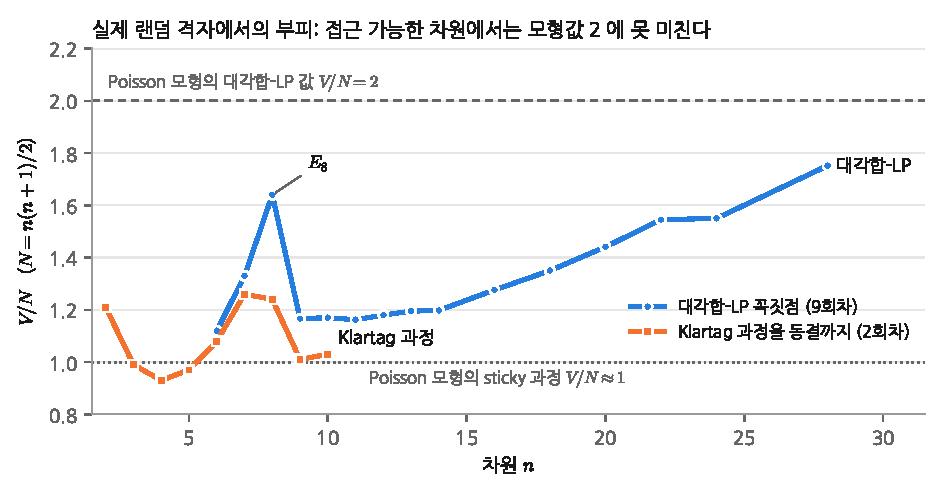
\includegraphics[width=0.86\textwidth]{figs/fig_VN.pdf}
\caption{실제 랜덤 격자에서 $V/N$ ($N=n(n+1)/2$). 파랑: 대각합-LP 꼭짓점(9회차; $n\ge16$ 은 큰 소수의 Goldstein--Mayer 격자), 주황: Klartag 과정을 동결까지(2회차). 점선은 Poisson 모형의 값. $n=8$ 의 봉우리는 LP 가 대부분 $E_8$ 에 도달하기 때문이다. 수치는 본문의 표와 같다.}\label{fig:VN}
\end{figure}
\begin{conjecture}[LP 추측; 점근적 진술로만]\tagJ\ Haar-랜덤 격자 $L$ 에 대해 $n\to\infty$ 에서 $V_{LP}(L)=(1+o(1))n^2$. 특히 $V_n\ge(1-o(1))n^2$.\end{conjecture}
이는 상수의 개선(현재 $\tfrac1{2e}$)일 뿐 차수의 개선이 아니다. 증명에는 ``한 타원체 위의 $N$ 개 격자벡터'' 통계가 필요하며 현재 기술 밖이다.

\subsection{비볼록 부분: 존재 임계값 (휴리스틱으로 강등)}
노름이 큰 $\theta\in K_v$ 는 곡률 보너스 $e^{\rho^2/8}$ 덕에 더 큰 부피를 준다. 모형에서:
\begin{itemize}
\item \tagM\ 정확한 쌍 공식: $\P(\theta,\theta'\in K_v)=\exp(-V\,\Phi(\delta/4))$, $\delta=|\theta-\theta'|$.
\item \tagL\ 음의 퍼셉트론(Montanari--Zhong--Zhou, arXiv:2110.15824): 존재 임계 $\delta_s(\kappa)=(1+o(1))\log|\kappa|/\Phi(\kappa)$, 한 LP 알고리즘의 임계 $\delta_{lin}(\kappa)=(1+o(1))/\Phi(\kappa)$. 국소 대응 $\kappa=-\rho/2$ 로 옮기면 존재 임계는 $V\approx2N(\log\rho+O(\log\log\rho))$.
\item \tagH\ 따라서 모형은 변형 스케일 $\rho$ 에서 $V\approx2N\log\rho$ 를 시사한다: $\rho^2\sim16\log N$ 에서 $\approx\tfrac12n^2\log\log n$, $\rho=n^a$ 에서 $\Theta(n^2\log n)$.
\end{itemize}
\textbf{심사에서 강등된 주장들} \tagF: (i) ``$V_n\ge cn^2\log n$'' 은 절단에 의존하는 휴리스틱이지 모형이 지지하는 추측이 아니다 --- 절단 없는 Poisson 모형은 $\sup V=\infty$ 이고, 가우스 근사의 유효 영역에는 $\rho\ll n^{1/4}$ 외에 작용소 노름 조건이 필요하며(지수적으로 가는 바늘은 구면 상계 $\rho^2N/4$ 조차 위반), 1차 모멘트 쪽($V\le CN\log\rho$)도 그물 논법으로는 $N\log(CN\rho^2)$ 까지만 나온다. (ii) ``알고리즘적/과정 기반 구성은 $\Theta(N)$ 을 넘지 못한다(통계--계산 간극)'' 는 근거가 없다 --- MZZ 는 한 알고리즘에 대해서만 간극을 증명했고, 재중심화하는 LP(극단 형식으로의 Voronoi 상승)는 모형 밖이다.

\subsection{구멍 확률로 본 장벽 (엄밀한 부분)}
$P_V:=\P_{\rm Haar}(L\cap B_V=\{0\})$ 로 두면 $V_n=\sup\{V:P_V>0\}$.
\begin{lemma}[근방 하계; Lemma N]\label{lem:N}\tagP\
$n\ge2$ 에 대해 $\ P_V\ \ge\ \exp(-2n^2\log n-n^2)\ $ for all $V\le V_n/2$.
\end{lemma}
(증명: 최적 격자 $L_0$ 의 최소벡터가 $\R^n$ 을 생성함을 보이고, $\{g:\|g-1\|_{op}\le\tfrac1{2n}\}\cdot L_0$ 가 단사임을 이용해 Siegel 의 부피 공식으로 Haar 측도를 계산. \texttt{rounds/R3\_process/notes.md} \S3.1, 3회차 심사 통과.)
\begin{corollary}\tagP\
만약 $V=V_n/2$ 에서 Poisson 형 상계 $P_V\le e^{-cV}$ 가 성립한다면 $V_n\le(4n^2\log n+2n^2)/c$. 즉 \emph{구멍 확률에 대한 Poisson 형 꼬리 상계 하나가 $V_n\le Cn^2\log n$ 을 증명한다.} 대우: $V_n\ge n^{2+\epsilon}$ 이면 $5n^2\log n\le V\le V_n/2$ 에서 $P_V\gg e^{-V/2}$ (강한 비-Poisson 성).
\end{corollary}
\begin{proposition}[거의 둥근 타원체에 대한 합집합 한계]\tagP\
$0<\rho<1$ 에 대해
$\ \mu\{\exists\,L\text{-free }A:\ \|A-I\|_{op}\le\rho,\ \det(A)^{-1/2}\ge V\}\le(1+\tfrac{4\rho n}{1-\rho})^{N}\,P_{V/\sqrt e}$.
\end{proposition}
현재 알려진 것은 $P_V\le Ce^{-c'n}$ ($V\ge cn$) 뿐이어서 위 한계는 쓸 수 없다. $k\le n-1$ 차 모멘트(Rogers)로는 $(k/V)^k$ 보다 작은 구멍 확률을 인증할 수 없으므로, $e^{-(n^2/2)\log n}$ 수준의 꼬리 한계는 새로운 입력을 요구한다.

\section{실패한 접근, 남은 빈틈, 다음 연구 과제}\label{sec:conclusion}

\subsection{실패했거나 강등된 접근 (이유와 함께)}
\begin{enumerate}
\item \textbf{고정점 없는 군으로 궤도를 키우기} (Venkatesh/AGZ 의 직접 확장). 실패 \tagP: Frobenius complement 의 구조정리 때문에 이득 $\tfrac12\sum\rho(g)^2\le24c/\varphi(c)=O(\log\log)$. 비가환군($SL_2(5)\times C_N$ 등)은 상수 4배만 준다.
\item \textbf{$\Delta=\Q$ 인 큰 군} (Weyl 군, $S_n$, Clifford 군/Barnes--Wall, $Co_0$ 자체). 실패 \tagP: 텐서형 격자 $W_\Z\otimes L$ 은 $\gamma_r/r<1$ 때문에 항상 불안정(순수 텐서가 지수적으로 많음).
\item \textbf{$PSL_2(p)$ ($p\equiv3\bmod4$), Heisenberg 군, $Sp_{2n}(p)$ ($n\ge2$), $SL_2(p)$ with $(p+1)/2$ 합성수}. 실패 \tagP/\tagH: 고정공간을 갖는 소수 위수 원소가 $a\ne b$ (unimodular 강직성) 또는 직선에서 $f\tau^2\to\tfrac12$.
\item \textbf{$SL_2(37)$}. 실패 \tagN: \S\ref{sec:weilcomp} --- $C_3$-고정 부분격자가 근을 가진 Niemeier 격자의 $\sqrt3$ 배.
\item \textbf{GGS 원분 접착에서 꼭대기를 피하는 지표 집합}으로 $M/C>M/\varphi(M)$. 개선 없음 \tagN: 약수 24개 이하의 모든 시험 모듈러스에서 admissible 데이터 0개; 일반 no-go 는 미증명.
\item \textbf{``Poisson 모형의 LP 값 $2N$ 이 격자에도 성립한다''}. 접근 가능한 차원에서는 거짓 \tagN: $n\le8$ 에서는 원리적으로 불가능, $n=14..28$ 에서 $V_{LP}/N=1.2$--$1.75$.
\item \textbf{``모형이 $V_n\asymp n^2\log n$ 을 예측한다'', ``과정 기반 구성은 $\Theta(n^2)$ 을 넘지 못한다''}. 심사에서 휴리스틱/사변으로 강등(\S\ref{sec:perceptron}).
\item \textbf{``Leech 텐서족이 $2.79\,n^2$ 을 준다''}. 정리가 아니라 휴리스틱으로 강등: $r\ge2$ 텐서족에 대한 등변 Klartag 정리가 없고, $k\approx r$ 에서는 호흡 모드 때문에 이득이 사라진다.
\item \textbf{소차원 규칙성에서 점근 공식 읽어내기}. 소차원의 좋은 격자(root, laminated, 큰 키싱 수)는 $V\gg n^2$ 인 예외적·퇴화 꼭짓점이고 점근 영역($V\sim wD$)과 다른 체제에 속한다. 얻은 구조적 교훈은 ``$V\approx$ 상수 $\times$ 독립 접촉 궤도 수 $\times$ 궤도 크기'' 라는 회계뿐이다.
\end{enumerate}

\subsection{정확히 어디서 막혔는가}
\begin{description}
\item[(G1) 텐서족에 대한 등변 Klartag 정리.] $A=M_r(\Delta)$, $r\ge2$ 일 때: 낮은 랭크 항을 포함한 평균값 공식(Steinitz 류 포함)의 완전한 증명, 비자유 궤도의 가중 계수, 그리고 $q=q_0(1+\tfrac{r-1/2}k)$ 의 호흡 모드 처리($k\ge Cr\log n$ 또는 대각합 없는 잡음). 이것이 있어야 Leech 족($p=13$)의 $2.79n^2$ 과 $p=61$ 의 조건부 상수가 정리가 된다.
\item[(G2) Weil 격자의 산술.] $p=61,73,157,\dots$ 에서 $N_{F/\Q}(q_F(\phi))\ge((p-1)/4)^2$ ($\forall\phi:C_p\to E$) 인가? 초등적으로는 $\deg\ge(p+3)/4$ 뿐. 유한 계산으로 결정 가능하지만 $p=61$ 은 120차원에서 노름 $\approx8$ 까지의 벡터를 $t$-원 전체에 대해 열거해야 한다.
\item[(G3) 접착 틀의 상계.] 모든 admissible 데이터에 $M/C\le K\,M/\varphi(M)$.
\item[(G4) LP 추측.] Haar-랜덤 격자에서 대각합-LP 꼭짓점의 부피 $(1+o(1))n^2$: ``한 타원체 위의 $N\gg n$ 개 격자벡터'' 의 기대 개수(Rogers 공식 밖).
\item[(G5) 구멍 확률.] $V\sim n^2\log n$ 에서 $P_V\le e^{-cV}$ --- 이것 하나가 $V_n\le Cn^2\log n$ 을 준다(Lemma N 과 결합).
\item[(G6) 문헌 확인.] Gross (1990), Nebe (1998) 원문 미열람; 정리 \ref{thm:quatAB} 의 새로움 미확인; Gargava 평균값 정리의 $s\ge2$ 경우 증명 세부.
\end{description}

\subsection{다음 연구 과제 (우선순위 순)}
\begin{enumerate}
\item \textbf{$p=61$ 결정.} (i) 12회차의 체계적 시험을 정수 연산으로 재현, (ii) BKZ/체질 수준의 격자 축소로 $W_{61}$ 의 $t$-원 전체에서 $Q_t$-최소벡터 탐색, (iii) Hilbert 모듈러 theta 급수($\Q(\sqrt{61})$, 무게 30)로 위반 계수의 소멸 여부를 조사. 안정이면 (G1)과 결합해 $n=120k$ 에서 Rezvyakova 상수의 약 63배(조건부).
\item \textbf{(G1) 증명.} 먼저 $p=13$ (Leech, $r=3$, class number 1, 경계 직선 1638개가 완전히 분류됨)에서. 대각합 없는 잡음 변형이 $k\approx r$ 에서도 작동하는지가 핵심 보조정리다.
\item \textbf{$p=73,157$} ($p\equiv1\bmod8$ 은 Galois 타원 몫이 없어 경계 벡터조차 알려져 있지 않다) 과 일반 $p$ 에 대한 구조적 논증: $C_m$-고정 부분격자 $=\sqrt m\,\times$(종수 $(p-1)/(2m)$ 곡선 $Y^2=X^{(p-1)/m+1}-X$ 의 같은 유형의 격자)라는 재귀 구조로 ``근의 존재'' 를 판정할 수 있는가.
\item \textbf{사원수 정리의 정리(整理)와 확장.} 정리 \ref{thm:quatAB} 를 논문 형태로 다듬고(Gargava 정리의 $s\ge2$ 세부 확인), 행렬 블록 경우(\S7)의 심사, 원분체와 결합해 $n^2\log\log n$ 의 명시적 상수 얻기.
\item \textbf{상계 쪽.} (G5)의 약한 형태 --- 예: 대칭이 없는 격자족에 한정한 구멍 확률의 Poisson 형 꼬리 --- 는 Venkatesh 의 추측에 대한 첫 증거가 된다. 반대로 $SL_2(p)$ 족이 안정이면 그 추측의 반례 후보다.
\end{enumerate}

\appendix
\section{사원수 대칭 Klartag 형 정리의 증명 전문 (6회차 개정본, 영문)}\label{app:proof}
{\small\sloppy
\hypertarget{r6-revised.-klartags-stochastic-ellipsoid-inside-the-invariant-forms-of-a-division-algebra-explicit-constants}{%
\subsection*{R6 (REVISED). Klartag\textquotesingle s stochastic ellipsoid inside the invariant forms of a division algebra: explicit constants}\label{r6-revised.-klartags-stochastic-ellipsoid-inside-the-invariant-forms-of-a-division-algebra-explicit-constants}}

\begin{quote}
\textbf{STATUS BOX} (revision of \texttt{proof.md} after two referee reports; both verdicts: \emph{correct modulo minor fixes}, no mathematical error found; the reviser re-derived Lemma 0.2, Lemma 1.3, Prop. 2.4, Lemma 3.3, Lemma 3.4, Prop. 3.5, Lemma 4.2 and the bookkeeping of §5 by hand once more).

\begin{itemize}
\tightlist
\item
  \textbf{Theorem A (Hurwitz, \(n=4k\), constant \(\frac3{2e}\)): PROVED, with cited inputs (L1)-(L3).}
\item
  \textbf{Theorem B (icosians, \(n=8k\), constant \(\frac{15}{4e}\)): PROVED, with cited inputs (L1)-(L3)} (see the caveat on (L1) for \(D_\mathbb R=\mathbb H\times\mathbb H\) in Remark 4.1a).
\item
  \textbf{Theorem C (general template): PROVED (with cited inputs (L1)-(L3)) in the case \(D_\mathbb R\cong\mathbb K^s\)} (all archimedean completions are division algebras) -\/- this is \textbf{Theorem C′} below; it contains A and B and was checked by both referees. \textbf{General case (\(D_{\mathbb R}\) with matrix blocks \(M_m(\mathbb K)\), \(m>1\)): PROVED UP TO THE FOLLOWING GAP:} the two missing ingredients (formula/minimum of \(q\); a Wishart-type angular lemma) are supplied with proofs in the new §7 of this revision (Lemma 7.1, Lemma 7.2), sanity-checked numerically (\texttt{check\_blocks.py}), but §7 was written during the revision and has \textbf{not been refereed}; it must be regarded as unverified until an independent check. No hypothesis "positive involution" is needed in §7 (finite groups are unitarisable at the real places).
\end{itemize}

\textbf{Cited inputs.} (L1) Gargava, arXiv:2107.04844, Theorem 16 (Siegel mean value theorem for \(g\mathcal O^k\), \(k\ge2\), \(\mathcal O\) an order {[}G, Def. 1{]} in a \(\mathbb Q\)-division algebra, \(f\in C_c\)): used as a black box; the quoted statement was compared with the text of {[}G{]} by both referees and by the reviser; its proof was NOT re-verified. All three theorems are conditional on it. (L2) Klartag, arXiv:2504.05042: the deterministic Lemma 2.1 and Lemma A.1 are used as stated; the proofs of Lemma 2.2, Prop. 2.3, Cor. 2.4, Lemma 3.1, Cor. 3.2, Lemma 3.3, Prop. 4.1, Prop. 4.2 are used with \(F_A\) replaced by the smaller space (13\(_\mathcal Q\)); the properties of \(F_A,\pi_A\) that these proofs use are listed and verified in §1-§3 (tag {[}V{]}); referee 1 re-read each of these proofs with the substitution and confirmed. (L3) Standard tools: Itô formula, Lévy characterisation, Dambis-Dubins-Schwarz, reflection principle, the GOE operator-norm tail bound (Vershynin, HDP, Cor. 4.4.8) as used in {[}K, Cor. 3.2{]}.

\textbf{Nature of the statements.} Purely asymptotic along \(n=4k\) (A), \(n=8k\) (B), \(n=k\delta\) (C′), \(k\to\infty\) with \((D,G)\) fixed; the \(o(1)\) is not effective and decays slowly (§6.6). Nothing is claimed for other \(n\). "Factor \(3\) / \(7.5\) over Rezvyakova" compares leading constants only. The bounds do NOT improve the order of magnitude: they are weaker than the \(c\,n^2\log\log n\) bounds of Abuya-Gargava-Zhao and Gargava-Groebner-Simkin for large \(n\) (those have an unspecified small \(c\)); what is gained is an explicit leading constant.
\end{quote}

Status tags: \textbf{{[}P{]}} proved here in full; \textbf{{[}V{]}} "verbatim": the cited proof of Klartag applies word for word once the listed
properties are checked (they are checked here); \textbf{{[}L{]}} quoted from the literature with exact reference and hypotheses; \textbf{{[}GAP{]}} not proved.
References: {[}K{]} Klartag, arXiv:2504.05042v2 (numbering of v2); {[}R{]} Rezvyakova, arXiv:2608.22590; {[}G{]} Gargava, \emph{Lattice packings
through division algebras}, arXiv:2107.04844; {[}V{]} Vance, arXiv:1105.3779. Numerical sanity checks: \texttt{check\_q.py} (same directory).

Normalisation: for a lattice \(L\subset\mathbb R^n\), \(V(L)=\sup\{\mathrm{Vol}(B)/\mathrm{covol}(L)\}\) over open origin-centred balls \(B\) with
\(B\cap L=\{0\}\); \(V_n=\sup_L V(L)\); packing density \(=V/2^n\). \(\kappa_n=\mathrm{Vol}(B^n)\).

\hypertarget{main-results}{%
\subsubsection*{Main results}\label{main-results}}

Let \(\mathbb K\in\{\mathbb R,\mathbb C,\mathbb H\}\), \(d=\dim_{\mathbb R}\mathbb K\in\{1,2,4\}\).

\textbf{Standing data (D).} \(D\) is a division algebra of dimension \(\delta\) over \(\mathbb Q\) such that \(D_{\mathbb R}:=D\otimes_{\mathbb Q}\mathbb R\cong\mathbb K^{s}\)
as \(\mathbb R\)-algebras (\(\delta=sd\)), and \(G\subset D^\times\) is a finite subgroup, \(w:=|G|\), whose \(\mathbb Q\)-span is \(D\).
Put \(\mathcal O:=\mathbb Z[G]\) (the \(\mathbb Z\)-span of \(G\)), and
\[D_k:=s\Big(k+\frac{d\,k(k-1)}2\Big)=\dim_{\mathbb R}\{(H_v)_{v\le s}:H_v\in \mathrm{Herm}_k(\mathbb K)\}.\]

\textbf{Theorem C′ (template, product-of-division-algebras case) {[}P modulo L{]}.} For data (D), as \(k\to\infty\) (\(D,G\) fixed), with \(n=k\delta\),
\[V_{n}\ \ge\ (1-o(1))\,\frac{w\,\delta\,k^2}{4e}\;=\;(1-o(1))\,\frac{w\,n^2}{4e\,\delta}\;=\;(1-o(1))\,\frac{w\,D_k}{2e}.\]
Moreover the lattice can be taken to be a \(G\)-invariant lattice \(\lambda g\mathcal O^k\), \(g\in GL_k(D_{\mathbb R})\).

\textbf{Theorem A (Hurwitz) {[}P modulo L{]}.} \(D=(\tfrac{-1,-1}{\mathbb Q})\), \(G=2T\) = the 24 Hurwitz units, \(\mathcal O\) = Hurwitz order, \(s=1\), \(\mathbb K=\mathbb H\),
\(\delta=4\), \(D_k=k(2k-1)\): for \(n=4k\to\infty\),
\[V_n\ \ge\ (1-o(1))\frac{24k^2}{e}=\Big(\frac{3}{2e}-o(1)\Big)n^2 .\]

\textbf{Theorem B (icosians) {[}P modulo L{]}.} \(D=(\tfrac{-1,-1}{\mathbb Q(\sqrt5)})\), \(G=2I\) (binary icosahedral group, \(w=120\)), \(\mathcal O=\mathbb Z[2I]\) (icosian ring),
\(s=2\), \(\mathbb K=\mathbb H\), \(\delta=8\), \(D_k=2k(2k-1)\): for \(n=8k\to\infty\),
\[V_n\ \ge\ (1-o(1))\frac{240k^2}{e}=\Big(\frac{15}{4e}-o(1)\Big)n^2 .\]

(Compare: {[}R{]} gives \((\frac1{2e}-o(1))n^2\) for all \(n\); A and B improve this explicit leading constant by the factors \(3\) and \(7.5\), along \(4\mid n\) resp. \(8\mid n\) only, and only asymptotically.)

\textbf{Relation to the literature (novelty NOT verified line by line).} The mechanism -\/- run Klartag\textquotesingle s process inside the forms invariant under a finite group acting freely, so that an orbit of \(w\) contact points costs one linear constraint -\/- is that of Abuya-Gargava-Zhao (arXiv:2606.05105) and Gargava-Groebner-Simkin (arXiv:2610.12619) for cyclic groups of roots of unity (cyclotomic fields), where it yields \(c\,n^2\log\log n\) with unspecified \(c\). What this note adds, to the best of our knowledge: (i) the non-commutative orders (Hurwitz, icosians; random lattices from {[}G, Thm 16{]}); (ii) explicit leading constants \(\frac{w}{4e\delta}\), via the identity \(P(x\otimes x)=L_{xx^*/d}\), i.e. the projected variance \(q(x)\ge q_0=\frac1\delta\) (Lemma 0.2), with \(q\equiv\frac14\) for Hurwitz; (iii) the angular Lemma 3.4 handling non-constant \(q\) (\(s\ge2\)). Neither referee nor the reviser checked whether those two papers already contain (i)-(iii).

\textbf{Literature inputs {[}L{]}} (everything else is proved below): (i) Gargava\textquotesingle s mean value theorem {[}G, Thm 16{]} (Section 4);

\begin{enumerate}
\def\labelenumi{(\roman{enumi})}
\setcounter{enumi}{1}
\tightlist
\item
  Klartag\textquotesingle s deterministic Lemma 2.1 and Lemma A.1 {[}K{]}, the GOE tail bound used in {[}K, Cor. 3.2{]} (Vershynin, HDP, Cor. 4.4.8),
  and standard stochastic calculus (Itô formula, Lévy characterisation, Dambis--Dubins--Schwarz, reflection principle) exactly as used in {[}K{]};
\item
  for Theorem B: the 120 unit icosians form a group (Conway--Sloane, SPLAG, Ch. 8 §2.1). This is also verified here by EXACT arithmetic in \(\mathbb Q(\sqrt5)\) (\texttt{check\_q.py}, part (2b): the monoid generated by the three generators of 0.1 has exactly 120 elements, all of reduced norm 1, contains \(-1,i,j,k\) and an element outside \(\mathbb Q\langle1,i,j,k\rangle\); a finite submonoid of a group is a group), so (iii) is in fact \textbf{{[}P, computer-checked{]}}.
\end{enumerate}

\textbf{Theorem C as posed by the orchestrator} (arbitrary \(D\) with positive involution, i.e. \(D_{\mathbb R}\cong\prod_v M_{m_v}(\mathbb K_v)\) with some \(m_v>1\),
e.g. cyclic algebras of degree \(\ge3\) from Amitsur\textquotesingle s list): not covered by §0-§5; see §7 (new in the revision, \textbf{un-refereed}). Under the hypothesis "\(G\) finite with \(\mathbb Q\)-span \(D\)"
the case \(D_\mathbb R\cong \mathbb K^s\) treated here is exactly: \(D=\mathbb Q\) (\(G=\pm1\), Klartag/Rezvyakova), \(D\) a cyclotomic field (\(G=\mu_m\)), or \(D\) a totally
definite quaternion algebra over a totally real field (\(G\subset D^1\): \(2T,2O,2I\), dicyclic groups). (Reason: if \(D\otimes_F F_v\) is a division algebra for every
archimedean place \(v\) of the centre \(F\), then either \(D=F\), and a field spanned by roots of unity is \(\mathbb Q\) or CM, or \(\dim_FD=4\) and all places are real and ramified.)

\begin{center}\rule{0.5\linewidth}{0.5pt}\end{center}

\hypertarget{setup}{%
\subsubsection*{0. Setup}\label{setup}}

\textbf{0.1 Algebra {[}P{]}.} \(\mathcal O=\mathbb Z[G]\) is a subring of \(D\) containing \(1\), finitely generated as a \(\mathbb Z\)-module, with \(\mathbb Q\mathcal O=D\):
an order in the sense of {[}G, Def. 1{]}. Fix the isomorphism \(D_{\mathbb R}\cong\mathbb K^s\), \(c\mapsto(c_v)_{v\le s}\). Every \(u\in G\) has finite order, hence
\(|u_v|=1\) for all \(v\) (\(|\cdot|\) is multiplicative on \(\mathbb K\)). \(D\) is a division algebra, so \(u-1\in D^\times\) for \(1\ne u\in G\), hence \((u-1)_v\neq0\) for all \(v\)
(invertible elements of \(D\) are invertible in \(D_\mathbb R\)).

\emph{Hurwitz:} \(D=\mathbb Q\langle1,i,j,k\rangle\), \(G=\{\pm1,\pm i,\pm j,\pm k,\tfrac12(\pm1\pm i\pm j\pm k)\}\), \(\mathbb Z[G]\) = Hurwitz order, \(\mathbb Q G=D\) since \(1,i,j,k\in G\).
\emph{Icosians:} \(K=\mathbb Q(\sqrt5)\), \(\tau=\frac{1+\sqrt5}2\), \(D=K\langle1,i,j,k\rangle\); \(D\) is a division algebra because \(x\bar x=x_0^2+\dots+x_3^2\in K\subset\mathbb R\)
is nonzero for \(x\ne0\). \(G=2I\) is generated by \(i\), \(\tfrac12(1+i+j+k)\), \(\tfrac12(\tau+\tau^{-1}i+j)\); it has order 120 and contains \(2T\ni 1,i,j,k\).
Its \(\mathbb Q\)-span \(A\) is a subalgebra (hence a division ring) properly containing \(\mathbb Q\langle1,i,j,k\rangle\); \(D\) is a left \(A\)-vector space, so
\(\dim_{\mathbb Q}A\) divides \(8\) and exceeds \(4\): \(A=D\). \(D_{\mathbb R}=\mathbb H\times\mathbb H\) via the two embeddings \(\sqrt5\mapsto\pm\sqrt5\) applied to coordinates.

\textbf{0.2 The Euclidean space and the action {[}P{]}.} \(E:=D_{\mathbb R}^k=\bigoplus_{v\le s}\mathbb K^k\), elements \(x=(x^{(v)})_v\), \(x^{(v)}\in\mathbb K^k\) \textbf{column} vectors;
\(n=\dim_{\mathbb R}E=k\delta\). Inner product \(\langle x,y\rangle=\sum_v\mathrm{Re}(x^{(v)*}y^{(v)})\), \(|x|^2=\sum_v\sum_{i\le k}|x^{(v)}_i|^2\) (the standard
Euclidean structure of \(\mathbb R^n\); \(x^*\) = conjugate transpose). \textbf{Conventions:} matrices \(M=(M_v)\in M_k(D_{\mathbb R})=\prod_vM_k(\mathbb K)\) act on the \textbf{left},
\(L_M x=(M_vx^{(v)})_v\); scalars \(c\in D_{\mathbb R}\) act on the \textbf{right}, \(R_cx=(x^{(v)}c_v)_v\). These commute. (This is the convention of {[}G{]}: lattices \(g\mathcal O^k\) are
right \(\mathcal O\)-modules; {[}V{]} uses the mirror convention, related by \(x\mapsto\bar x\).) For \(u\in G\), \(R_u\) is orthogonal because \(|u_v|=1\).
\(G\) acts \textbf{freely} on \(E\setminus\{0\}\): if \(xu=x\), \(x^{(v)}_i\ne0\), then \(x^{(v)}_i(u_v-1)=0\) in the division ring \(\mathbb K\), so \((u-1)_v=0\), so \(u=1\) by 0.1.
Hence every \(G\)-orbit in \(E\setminus\{0\}\) has exactly \(w\) elements.

\textbf{0.3 Invariant forms.} Let \(\mathrm{Sym}_n\) be the symmetric endomorphisms of \(E\) with \(\langle A,B\rangle=\mathrm{Tr}[AB]\), and
\[\mathcal Q:=\{A\in\mathrm{Sym}_n:\ R_u^{T}AR_u=A\ \ \forall u\in G\}.\]

\textbf{Lemma 0.1 {[}P{]}.} \(\mathcal Q=\{L_H:\ H=(H_v)_v,\ H_v\in\mathrm{Herm}_k(\mathbb K)\}\); \(\dim\mathcal Q=D_k\); \(\mathrm{Id}\in\mathcal Q\); and for such \(H,H'\):
\(\langle L_H,L_{H'}\rangle=d\sum_v\mathrm{Re\,tr}(H_vH'_v)\).

\emph{Proof.} \(R_u\) is orthogonal, so \(R_u^TAR_u=A\) iff \(AR_u=R_uA\). The map \(c\mapsto R_c\) is \(\mathbb R\)-linear on \(D_{\mathbb R}\) and the \(\mathbb R\)-span of \(G\) is
\(D_{\mathbb R}\) (the \(\mathbb Q\)-span is \(D\)). So \(A\in\mathcal Q\) iff \(A\) is symmetric and commutes with all \(R_c\), \(c\in D_{\mathbb R}\), i.e. is right \(D_{\mathbb R}\)-linear.
Commuting with the idempotents \(e_v\), \(A\) preserves each summand \(\mathbb K^k\) and is right \(\mathbb K\)-linear there, hence \(A(x)=A(\sum_ie_ix_i)=\sum_iA(e_i)x_i\)
is left multiplication by a matrix: \(A=L_M\), \(M\in\prod_vM_k(\mathbb K)\). Since \((M_vx)^*=x^*M_v^*\), \(\langle L_Mx,y\rangle=\langle x,L_{M^*}y\rangle\); as
\(M\mapsto L_M\) is injective, \(L_M\) is symmetric iff \(M=M^*\). Conversely every \(L_H\) commutes with every \(R_u\). The dimension is \(s(k+d\binom k2)\).
Finally \(\mathrm{Tr}_{\mathbb R}L_M=d\sum_v\mathrm{Re\,tr}M_v\) (for \(c\in\mathbb K\), left multiplication by \(c\) on \(\mathbb K=\mathbb R^d\) has trace \(d\,\mathrm{Re}\,c\);
off-diagonal entries do not contribute). \(\square\)

\textbf{Lemma 0.2 (projection and the constant \(q\)) {[}P{]}.} Let \(P:\mathrm{Sym}_n\to\mathrm{Sym}_n\) be the orthogonal projection onto \(\mathcal Q\). Then

\begin{enumerate}
\def\labelenumi{(\alph{enumi})}
\tightlist
\item
  \(P(B)=\frac1w\sum_{u\in G}R_uBR_u^T\); in particular \(\|P(B)\|_{op}\le\|B\|_{op}\) and \(P(xu\otimes xu)=P(x\otimes x)\) for \(u \in G\);
\item
  \(P(x\otimes x)=L_{K}\) with \(K_v=\frac1d\,x^{(v)}x^{(v)*}\);
\item
  \(|P(x\otimes x)|^2=\frac1d\sum_v|x^{(v)}|^4=q(x)|x|^4\), where, with \(u_v:=|x^{(v)}|^2/|x|^2\) and \(q_0:=\frac1{\delta}\),
  \[q(x)=\frac1d\sum_vu_v^2=q_0\Big(1+s\sum_{v}\big(u_v-\tfrac1s\big)^2\Big)\in[q_0,\ sq_0].\]
  \emph{Hurwitz (\(s=1\), \(d=4\)): \(q\equiv\frac14\). Icosians (\(s=2,d=4\)): \(q=\frac14(u_1^2+u_2^2)\), \(q_0=\frac18\).}
\end{enumerate}

\emph{Proof.} (a) \(B\mapsto R_uBR_u^T\) is an orthogonal map of \(\mathrm{Sym}_n\) with inverse given by \(u^{-1}\), so the average is self-adjoint; it is idempotent with
image \(\mathcal Q\): it is \(P\). The norm bound is the triangle inequality; \(xu\otimes xu=R_u(x\otimes x)R_u^T\). (b) \(K_v\) is Hermitian, and for \(B=L_H\in\mathcal Q\),
by Lemma 0.1 and \(\mathrm{Re\,tr}(XY)=\mathrm{Re\,tr}(YX)\): \(\langle L_K,L_H\rangle=\sum_v\mathrm{Re\,tr}(x^{(v)}x^{(v)*}H_v)=\sum_v\mathrm{Re}(x^{(v)*}H_vx^{(v)}) =\langle L_Hx,x\rangle=\langle B,x\otimes x\rangle\). (c) \(|L_K|^2=d\sum_v d^{-2}\mathrm{Re\,tr}(x^{(v)}(x^{(v)*}x^{(v)})x^{(v)*})=\frac1d\sum_v|x^{(v)}|^4\) since
\(x^{(v)*}x^{(v)}=|x^{(v)}|^2\) is a real scalar; and \(\sum_vu_v^2=\frac1s+\sum_v(u_v-\frac1s)^2\) as \(\sum_v u_v=1\). \(\square\)

(\texttt{check\_q.py}: \(D_k=1,6,15\) for Hurwitz \(k=1,2,3\); \(2,12\) for icosians \(k=1,2\); \(q=0.25\) to 12 digits; \(P(x\otimes x)=L_{xx^*/4}\) to \(10^{-15}\).)

\textbf{0.4 Lattices {[}P{]}.} A \emph{\(G\)-lattice} is \(L=\lambda\,g\,\mathcal O^k\), \(\lambda>0\), \(g\in GL_k(D_{\mathbb R})\) (\(\mathcal O^k\subset D^k\subset E\)). It is a lattice in \(E\)
and \(LG=L\) (right multiplication commutes with \(L_g\) and \(\mathcal O u=\mathcal O\)). If \(A\in\mathcal Q\) is positive definite, \(\sqrt A\in\mathcal Q\)
(a polynomial in \(A\)), \(\sqrt A=L_h\), \(h\in GL_k(D_\mathbb R)\), so \(\sqrt A\,L\) is again a \(G\)-lattice.

\begin{center}\rule{0.5\linewidth}{0.5pt}\end{center}

\hypertarget{the-process-in-mathcal-q-klartag-2}{%
\subsubsection*{\texorpdfstring{1. The process in \(\mathcal Q\) (Klartag §2)}{1. The process in \textbackslash mathcal Q (Klartag §2)}}\label{the-process-in-mathcal-q-klartag-2}}

Let \(L\subset\mathbb R^n\) be a lattice and \(\mathcal Q\subseteq\mathrm{Sym}_n\) \textbf{any} linear subspace containing \(\mathrm{Id}\). For \(A\in\mathrm{Sym}_n\) put
\[F_A:=\{B\in\mathcal Q:\ Bx\cdot x=0\ \ \forall x\in\partial E_A\cap L\},\qquad \pi_A:=\text{orthogonal projection of }\mathrm{Sym}_n\text{ onto }F_A .\tag{13$_\mathcal Q$}\]
(Klartag\textquotesingle s (13) is the case \(\mathcal Q=\mathrm{Sym}_n\).) Let \((W_t)\) be a Dyson Brownian motion in \(\mathrm{Sym}_n\), as in {[}K{]}.

\textbf{Proposition 1.1 (= {[}K, Lemma 2.2, Prop. 2.3, Cor. 2.4{]} with (13) replaced by (13\(_\mathcal Q\))) {[}V{]}.} Let \(a_0>0\) with \(a_0\mathrm{Id}\) \(L\)-free.
There is a continuous adapted process \((A_t)_{t\ge0}\) with (A)--(E) of {[}K, Prop. 2.3{]} and \(A_t=a_0\mathrm{Id}+\int_0^t\pi_s(dW_s)\), \(\pi_s=\pi_{A_s}\). In addition \(A_t\in\mathcal Q\) for all \(t\).

\emph{Proof.} We list what the proofs in {[}K{]} use about \(F_A,\pi_A\) and check it for (13\(_\mathcal Q\)).

\begin{itemize}
\tightlist
\item
  {[}K, Lemma 2.1{]} is a deterministic statement about continuous families in \(\mathrm{Sym}_n\); no change.
\item
  {[}K, Lemma 2.2{]} uses: (i) \(\pi_{M_0}\) is an orthogonal projection, not identically zero when \(F_{M_0}\ne0\), \textbf{hence} there is \(x_0\) with \(\pi_{M_0}(x_0\otimes x_0)\ne0\)
  (true since the \(x\otimes x\) span \(\mathrm{Sym}_n\)); then \(\pi_{M_0}(W_t)x_0\cdot x_0=\langle W_t,\pi_{M_0}(x_0\otimes x_0)\rangle\) is a nondegenerate one-dimensional Brownian
  motion, giving (16); (ii) \(Bx\cdot x=0\) for \(B\in F_{M_0}\), \(x\in\partial E_{M_0}\cap L\) (true by definition), giving (11). Nothing else.
\item
  {[}K, Prop. 2.3{]} uses in addition: \(F_A\) depends on \(A\) only through the contact set \(\partial E_A\cap L\) (true), the bounds (7),(8) for lattices (unchanged),
  and the strong Markov property of \(W\). The recursion stops when \(F_{\tau_{i-1}}=\{0\}\). Each step adds at least one contact point (Lemma 2.1(C)), so \(M\le\tilde C_L\).
  (In fact \(M\le\dim\mathcal Q\): if \(x\) is a new contact point at time \(\tau_i\), then \(A_tx\cdot x>1\) for \(\tau_{i-1}\le t<\tau_i\) and \(A_{\tau_i}x\cdot x=1\), so \(\langle A_{\tau_i}-A_{\tau_{i-1}},x\otimes x\rangle\ne0\) with \(A_{\tau_i}-A_{\tau_{i-1}}\in F_{\tau_{i-1}}\); hence \(F_{\tau_i}\subsetneq F_{\tau_{i-1}}\), the dimension drops strictly at each step. For \(G\)-lattices the whole orbit \(xG\) becomes contact at the same time, Lemma 1.3.)
\item
  {[}K, Cor. 2.4{]} uses only (A),(B) and boundedness of \(M\).
  Finally \(A_t-a_0\mathrm{Id}\) is a sum of elements \(\pi_{\tau_{i-1}}(\cdot)\in F_{\tau_{i-1}}\subseteq\mathcal Q\) and \(\mathrm{Id}\in\mathcal Q\). \(\square\)
\end{itemize}

\textbf{Remark 1.2.} \(\pi_s=\pi_sP\) and \(\pi_s(dW_s)=\pi_s(d(PW)_s)\) where \(PW\) is a standard Brownian motion in \(\mathcal Q\): this is "Klartag\textquotesingle s process run inside \(\mathcal Q\)".
Writing it with the ambient Dyson motion makes all of {[}K, §2--3{]} literally applicable.

From now on \(\mathcal Q\) is the space of 0.3 and \(L\) is a \(G\)-lattice.

\textbf{Lemma 1.3 (orbit counting) {[}P{]}.} Almost surely for all \(t\): \(\partial E_t\cap L\) is \(G\)-invariant and
\[N_t:=\dim F_t=\mathrm{Tr}[\pi_t]\ \ge\ D_k-\frac{|\partial E_t\cap L|}{w}.\]
\emph{Proof.} \(A_t\in\mathcal Q\) gives \(A_t(xu)\cdot(xu)=A_tx\cdot x\), and \(Lu=L\). \(F_t\) is the orthogonal complement in \(\mathcal Q\) of \(\mathrm{span}\{P(x\otimes x):x\in\partial E_t\cap L\}\)
(as \(Bx\cdot x=\langle B,P(x\otimes x)\rangle\) for \(B\in\mathcal Q\)). By Lemma 0.2(a) \(P(x\otimes x)\) is constant on \(G\)-orbits, and by 0.2 all orbits in \(L\setminus\{0\}\)
have size \(w\); so the span has dimension \(\le|\partial E_t\cap L|/w\). \(\square\)

\hypertarget{volume-klartag-3}{%
\subsubsection*{2. Volume (Klartag §3)}\label{volume-klartag-3}}

\textbf{Lemma 2.1 (= {[}K, Lemma 3.1{]}, Maurey) {[}V{]}.} \(A_t=a_0\mathrm{Id}+\frac12(W^{(1)}_t+W^{(2)}_t)\) with two Dyson Brownian motions in \(\mathrm{Sym}_n\).
\emph{Proof (written out).} \(\pi_s\) is an adapted (piecewise constant, by Prop. 1.1) orthogonal projection of \(\mathrm{Sym}_n\), so \(U_s:=2\pi_s-\mathrm{Id}\) is an adapted orthogonal transformation of \(\mathrm{Sym}_n\). Put \(W^{(1)}=W\), \(W^{(2)}_t=\int_0^tU_s(dW_s)\). \(W^{(2)}\) is a continuous martingale in \(\mathrm{Sym}_n\) with \(d[\langle W^{(2)},B\rangle,\langle W^{(2)},B'\rangle]_t=\langle U_s^TB,U_s^TB'\rangle dt=\langle B,B'\rangle dt\), so it is a Dyson Brownian motion by Lévy\textquotesingle s characterisation, and \(\frac12(W^{(1)}_t+W^{(2)}_t)=\int_0^t\pi_s(dW_s)=A_t-a_0\mathrm{Id}\). Nothing about the range of \(\pi_s\) is used, so {[}K, Cor. 3.2{]} holds with Klartag\textquotesingle s same constants. \(\square\)

\textbf{Corollary 2.2 (= {[}K, Cor. 3.2{]}) {[}V{]}.} For \(t>0\), \(r\ge\sqrt{tn}\): \(\ \mathbb P(\|A_t-a_0\mathrm{Id}\|_{op}\ge C_0r)\le Ce^{-r^2/t}\), with Klartag\textquotesingle s universal \(C_0,C\).

\textbf{Lemma 2.3 (= {[}K, Lemma 3.3{]}) {[}V{]}.} \(\mathbb E\log\det A_T\le n\log a_0-\frac12\int_0^T\mathbb E[\|A_t\|_{op}^{-2}N_t]\,dt\), \(N_t=\mathrm{Tr}[\pi_t]=\dim F_t\).
\emph{Proof (the points where \(\pi_t\) enters, written out).} Itô\textquotesingle s formula for \(\log\det\) (\(\nabla\log\det A=A^{-1}\), \(\nabla^2\log\det A(B,B)=-\mathrm{Tr}[A^{-1}BA^{-1}B]\)) and \(dA_t=\pi_t(dW_t)\) give \(d\log\det A_t=\langle\pi_t(A_t^{-1}),dW_t\rangle-\frac12\delta_tdt\), \(\delta_t=\sum_\alpha\mathrm{Tr}[A_t^{-1}E_\alpha A_t^{-1}E_\alpha]\) for an orthonormal basis \((E_\alpha)\) of \(F_t\). In an orthonormal eigenbasis of \(A_t\) (eigenvalues \(\lambda_i>0\)): \(\mathrm{Tr}[A_t^{-1}EA_t^{-1}E]=\sum_{i,j}E_{ij}^2/(\lambda_i\lambda_j)\ge\|A_t\|_{op}^{-2}|E|^2\), so \(\delta_t\ge\|A_t\|_{op}^{-2}\dim F_t\) -\/- valid for an arbitrary orthogonal projection \(\pi_t\). The stochastic integral has zero expectation because \(|\pi_t(A_t^{-1})|\le|A_t^{-1}|\) and \(\mathbb E\int_0^T|A_t^{-1}|^2dt<\infty\) exactly as in {[}K{]} ((32) and Cor. 3.2, which do not involve \(F_t\)). \(\square\)

\textbf{Proposition 2.4 (quantitative Prop. 3.4; cf. {[}R, Prop. 2{]}) {[}P{]}.} Let \(T>0\), \(\rho\ge0\), \(1\le a_0\le1+\frac{3\rho}n\). Then
\[\mathbb E\log\det A_T\le n\log a_0-\frac{D_kT}2+\frac1{2w}\int_0^T\mathbb E|\partial E_t\cap L|\,dt+C'D_k\big(\tfrac{\rho}{n}T+n^{1/2}T^{3/2}+e^{-n}T\big),\]
\(C'\) universal. (As \(D_k\le n^2\) the error is \(\le C'(\rho nT+n^{5/2}T^{3/2}+n^2e^{-n}T)\), the form of {[}R, Prop. 2{]}; no upper bound on \(T\) is needed.)

\emph{Proof.} Let \(S_t=\{\|A_t-a_0\mathrm{Id}\|_{op}\le C_0\sqrt{tn}\}\); \(\mathbb P(S_t^c)\le Ce^{-n}\) (Cor. 2.2, \(r=\sqrt{tn}\)). On \(S_t\),
\(\|A_t\|_{op}^{-2}\ge(1+\frac{3\rho}n+C_0\sqrt{tn})^{-2}\ge1-\frac{6\rho}n-2C_0\sqrt{tn}\). Since \(0\le N_t\le D_k\), pointwise \(\|A_t\|_{op}^{-2}N_t\ge N_t-(\frac{6\rho}n+2C_0\sqrt{tn})D_k-\mathbf 1_{S_t^c}D_k\) (on \(S_t\) by the previous line, on \(S_t^c\) trivially), so
\(\mathbb E[\|A_t\|_{op}^{-2}N_t]\ge\mathbb E[N_t]-(\frac{6\rho}n+2C_0\sqrt{tn})D_k-CD_ke^{-n}\). Integrate over \([0,T]\), insert into Lemma 2.3, and use Lemma 1.3. \(\square\)

\hypertarget{contact-points-klartag-4}{%
\subsubsection*{3. Contact points (Klartag §4)}\label{contact-points-klartag-4}}

\textbf{Proposition 3.1 (= {[}K, Prop. 4.1{]} with the projected variance) {[}P{]}.} For fixed \(T>0\) and \(0\ne x\in L\),
\[\mathbb P(x\in\partial E_T)\le2\,\mathbb P\Big(Z\ge\frac{1}{\sqrt{q(x)T}}\Big(a_0-\frac1{|x|^2}\Big)\Big),\qquad Z\sim N(0,1).\]
\emph{Proof.} As in {[}K{]}: \(M_t=\langle A_t,x\otimes x\rangle-1\), \(dM_t=\langle dW_t,\pi_t(x\otimes x)\rangle\). Since \(F_t\subseteq\mathcal Q\), \(\pi_t=\pi_tP\), so
\([M]_t=\int_0^t|\pi_sP(x\otimes x)|^2ds\le t\,|P(x\otimes x)|^2=t\,q(x)|x|^4\) by Lemma 0.2(c). The rest of Klartag\textquotesingle s proof (Dambis--Dubins--Schwarz and the reflection principle)
goes through with \(|x|^4\) replaced by \(q(x)|x|^4\): \(\mathbb P(x\in\partial E_T)\le2\mathbb P(B_{Tq(x)|x|^4}\ge a_0|x|^2-1)\). \(\square\)

Let \(\Phi\) be as in {[}K, (48){]}, \(\mathcal D_t=\{x:(a_0-C_0\sqrt{tn})|x|^2<1\}\), and
\[K_t(L):=\sum_{0\ne x\in L\cap\mathcal D_t}\Phi\Big(\frac{1}{\sqrt{q(x)t}}\Big(a_0-\frac1{|x|^2}\Big)\Big).\]

\textbf{Proposition 3.2 (= {[}K, Prop. 4.2{]}) {[}V{]}.} \(\mathbb E|\partial E_t\cap L|\le2K_t(L)+Ce^{-cn}\). (Proof: verbatim {[}K, proof of Prop. 4.2{]}; it uses Prop. 3.1 for \(x\in L\cap\mathcal D_t\), the bound (49) \(\mathbb P(Z\ge r)\le\Phi(r)\) together with \(a_0-|x|^{-2}\ge0\), Cor. 2.2 for \(\mathbb P(\overline{E_t}\not\subseteq\mathcal D_t)\le Ce^{-n}\), and the bound {[}K, (8){]} \(|\partial E_t\cap L|\le2(2^n-1)\) for lattices. Recall {[}K, (48){]}: \(\Phi(r)=\min\{\frac12,\frac{1}{\sqrt{2\pi}r}e^{-r^2/2}\}\), the two bounds used in Lemma 3.3.)

\textbf{Lemma 3.3 (integral lemma; = {[}R, Lemma 1{]}, reproved with uniformity) {[}P{]}.} For every \(\varepsilon>0\) there is \(\eta\in(0,\frac14]\) such that for all \(n\ge1/\eta\), \(S>0\), \(Y>1\) with
\[n\sqrt S\ge1/\eta,\qquad n^3S^2\le\eta,\qquad Y\sqrt S\le\eta,\]
we have, with \(m=\frac{n+2}2\),
\[\int_0^S\frac{n\sqrt\sigma}2\int_0^Y\Phi(y)\,(1-y\sqrt\sigma)^{-m}\,dy\,d\sigma\ \le\ (1+\varepsilon)\frac8{n^2}e^{n^2S/8}.\]
\emph{Proof.} Put \(a=n\sqrt S/2\), \(\epsilon_1=Y\sqrt S\), \(\beta=1-2mS\); note \(mS\le nS=(n^3S^2)^{1/2}n^{-1/2}\le\eta\le\frac14\) (using \(n\ge1/\eta\ge4\)), hence \(\beta\ge\frac12\), \(\epsilon_1\le\eta\le\frac14\) (so \(y\sqrt\sigma\le\frac12\) below) and \(a\ge\frac1{2\eta}\). For \(0\le u\le\frac12\), \(-\log(1-u)\le u+u^2\), so for
\(y\le Y,\sigma\le S\): \((1-y\sqrt\sigma)^{-m}\le\exp(\tfrac n2y\sqrt\sigma+\epsilon_1+my^2S)\).
\emph{Range \(0\le y\le1\)} (\(\Phi\le\frac12\)): contribution \(\le\frac{n\sqrt S}4\,S\,e^{\epsilon_1+mS}e^{n\sqrt S/2}=\frac8{n^2}e^{n^2S/8}\cdot\frac{a^3}{4}e^{\epsilon_1+mS}e^{a-a^2/2}\), and \(a^3e^{a-a^2/2}\to0\).
\emph{Range \(1\le y\le Y\)} (\(\Phi(y)\le e^{-y^2/2}/(\sqrt{2\pi}y)\)): integrating first in \(\sigma\) (substitute \(\sigma=v^2\)),
\(\int_0^S\frac{n\sqrt\sigma}2e^{ny\sqrt\sigma/2}d\sigma=\int_0^{\sqrt S}nv^2e^{nyv/2}dv\le nS\cdot\frac2{ny}e^{ay}=\frac{2S}ye^{ay}\). Hence the contribution is at most
\[e^{\epsilon_1}\,2S\int_1^Y\frac{1}{\sqrt{2\pi}\,y^2}e^{-\beta y^2/2+ay}dy=e^{\epsilon_1}\,2S\,e^{a^2/(2\beta)}\int_1^Y\frac{1}{\sqrt{2\pi}y^2}e^{-\frac\beta2(y-a/\beta)^2}dy .\]
Here \(\frac{a^2}{2\beta}=\frac{n^2S}8+\frac{a^2}{2}\frac{2mS}{\beta}=\frac{n^2S}8+O(n^3S^2)\). Split the last integral at \(y_0=a(1-a^{-1/2})\): for \(y\ge y_0\), \(y^{-2}\le a^{-2}(1-a^{-1/2})^{-2}\) and
the Gaussian integral is \(\le\beta^{-1/2}\); for \(1\le y<y_0\), \(y^{-2}\le1\) and \(|y-a/\beta|\ge a^{1/2}\), giving \(\le\beta^{-1/2}e^{-\beta a/2}=o(a^{-2})\).
So the contribution is \(\le(1+o(1))\frac{2S}{a^2}e^{n^2S/8}=(1+o(1))\frac8{n^2}e^{n^2S/8}\), where every "\(o(1)\)" is bounded by an explicit function of \(\eta\) tending to \(0\) as \(\eta\to0\) (the tail bound used is \(\mathbb P(Z\ge u)\le\frac12e^{-u^2/2}\)). The dominant relative error is \((1-a^{-1/2})^{-2}-1=O(a^{-1/2})\): in the application \(a\asymp\sqrt{\log n}\), so the lemma as proved gives the factor \(1+O((\log n)^{-1/4})\) (a split at \(a/2\) with a second-order expansion would give \(O(1/\log n)\); not needed, only \(o(1)\) is used). \(\square\)
(\texttt{check\_q.py} (4): ratio LHS/RHS \(=1.045,1.017,1.013\) for \(n=10^5,10^7,10^9\), \(S=16\log n/n^2\), \(Y=2\sqrt n\).)

\textbf{Lemma 3.4 (angular lemma) {[}P{]}.} Let \(u=(u_1,\dots,u_s)\sim\mathrm{Dirichlet}(a,\dots,a)\) and \(b\) an integer with \(0\le b<a\). Then
\[\mathbb E\exp\Big(\frac{bs}{2}\sum_v\big(u_v-\tfrac1s\big)^2\Big)\le\Big(1-\frac ba\Big)^{-bs}.\]
\emph{Proof.} Let \(x_v=su_v-1\in(-1,s-1]\), \(\sum_vx_v=0\). For \(x\in(-1,s-1]\): \(\log(1+x)\le x-\frac{x^2}{2s}\) (for \(x\le0\): \(\log(1+x)\le x-\frac{x^2}2\); for \(x\ge0\):
\(\log(1+x)\le x-\frac{x^2}{2(1+x)}\) and \(1+x\le s\)). Summing, \(\sum_v\log(su_v)\le-\frac1{2s}\sum_vx_v^2=-\frac s2\sum_v(u_v-\frac1s)^2\), i.e.
\(\exp(\frac{bs}2\sum_v(u_v-\frac1s)^2)\le\prod_v(su_v)^{-b}\). By the Dirichlet integral, for \(b<a\),
\[\mathbb E\prod_v(su_v)^{-b}=s^{-bs}\frac{\Gamma(a-b)^s\,\Gamma(sa)}{\Gamma(a)^s\,\Gamma(sa-sb)}=\frac{\prod_{i=1}^{bs}(a-\frac is)}{\prod_{j=1}^{b}(a-j)^s}\le\Big(\frac a{a-b}\Big)^{bs}.\qquad\square\]
(For \(s=1\) the statement is trivial. Checked numerically in \texttt{check\_q.py} (3).)

\textbf{Proposition 3.5 (shell integral; replaces {[}K, Lemma 4.3{]} and {[}R, Prop. 1{]}) {[}P{]}.} Let \(\rho=\rho(n)\ge1\), \(\rho=o(\sqrt n)\), \(\alpha=(1-\frac\rho n)^{-2}\),
\(R_t=\{x:\frac1\alpha\le|x|^2<\frac1{\alpha-C_0\sqrt{tn}}\}\), and let \(z=z(n)\) satisfy \(\log n\le z\le 3\log n\); put \(T=\frac{8z}{q_0n^2}\). Then, as \(k\to\infty\) (\(D,G\) fixed),
\[\frac1{\kappa_n}\int_0^T\!\!\int_{R_t}\Phi\Big(\frac{1}{\sqrt{q(x)t}}\Big(\alpha-\frac1{|x|^2}\Big)\Big)dx\,dt\ \le\ (1+o(1))\,e^{-\rho}\,\frac{8}{q_0n^2}\,e^{z}.\]
\emph{Proof.} \(q\) is \(0\)-homogeneous. In polar coordinates \(x=r\omega\) (\(\sigma\) = uniform probability on \(S^{n-1}\)), substituting \(y=(q(\omega)t)^{-1/2}(\alpha-r^{-2})\) exactly as in
{[}K, proof of Lemma 4.3{]}, the inner integral equals
\[\int_{S^{n-1}}\frac{n\sqrt{q(\omega)t}}2\,\alpha^{-\frac{n+2}2}\int_0^{C_0\sqrt{n/q(\omega)}}\Phi(y)\Big(1-\frac{y\sqrt{q(\omega)t}}{\alpha}\Big)^{-\frac{n+2}2}dy\,d\sigma(\omega).\]
Use \(\alpha\ge1\), integrate in \(t\) and substitute \(\sigma=q(\omega)t\): by Lemma 3.3 with \(S=q(\omega)T\in[q_0T,sq_0T]\), \(Y=C_0\sqrt{n/q(\omega)}\)
(\(n\sqrt S\ge\sqrt{8z}\to\infty\), \(n^3S^2\le64s^2z^2/n\to0\), \(Y\sqrt S=C_0\sqrt{nT}\to0\), uniformly in \(\omega\)) the left side is at most
\[(1+o(1))\,\alpha^{-\frac{n+2}2}\,\frac8{n^2}\int_{S^{n-1}}\frac{1}{q(\omega)}e^{n^2q(\omega)T/8}d\sigma(\omega).\]
Now \(\alpha^{-(n+2)/2}=(1-\frac\rho n)^{n+2}\le e^{-\rho}\), \(q\ge q_0\), and by Lemma 0.2(c) \(n^2qT/8=z(1+s\sum_v(u_v-\frac1s)^2)\). For \(\omega\) uniform on the sphere,
\((u_v)_v\sim\mathrm{Dirichlet}(\frac{kd}2,\dots,\frac{kd}2)\). Lemma 3.4 with \(b=\lceil2z\rceil\), \(a=\frac{kd}2\) gives
\(\int e^{zs\sum_v(u_v-1/s)^2}d\sigma\le(1-\frac ba)^{-bs}=\exp(O(s\log^2n/k))=1+o(1)\). (For \(s=1\) this step is empty: \(q\equiv q_0\).) \(\square\)

\hypertarget{random-g-lattices-klartag-5}{%
\subsubsection*{\texorpdfstring{4. Random \(G\)-lattices (Klartag §5)}{4. Random G-lattices (Klartag §5)}}\label{random-g-lattices-klartag-5}}

\textbf{Theorem 4.1 (Gargava {[}G, Theorem 16 and Remark 17{]}) {[}L{]}.} Let \(D\) be a \(\mathbb Q\)-division algebra, \(\mathcal O\subseteq D\) an order, \(k\ge2\), \(\mathsf G=SL_k(D_{\mathbb R})\)
(unit-norm elements of \(M_k(D_\mathbb R)\)), \(\Gamma=SL_k(\mathcal O)\), \(dg\) the \(\mathsf G\)-invariant probability measure on \(\mathsf G/\Gamma\). Then for \(f\in C_c(D_{\mathbb R}^k)\):
\(\int_{\mathsf G/\Gamma}\sum_{v\in g\mathcal O^k\setminus\{0\}}f(v)\,dg=\int_{D_{\mathbb R}^k}f(x)\,dx\), \(dx\) = the Lebesgue measure giving \(\mathcal O^k\) covolume \(1\).
\textbf{Remark 4.1a (how the citation was checked; conventions; caveats).} (i) The statement above is {[}G, Thm 16{]} verbatim: \(\mathsf G=\{a\in M_k(D_\mathbb R):N(a)=1\}\), \(\Gamma=\{a\in M_k(\mathcal O):N(a)=1\}\) {[}G, §1.2{]}, \(\mathsf G/\Gamma\) carries a unique \(\mathsf G\)-invariant probability measure {[}G, Prop. 14{]}, "order" is {[}G, Def. 1{]} (finitely generated \(\mathbb Z\)-module, \(\mathbb Q\otimes\mathcal O=D\), closed under multiplication, \(1\in\mathcal O\) -\/- satisfied by \(\mathbb Z[G]\), 0.1; maximality is not required). (ii) Side conventions: {[}G{]} identifies \(\mathsf G/\Gamma\simeq\{g\mathcal O^k\}\) (matrices act on the left of \(\mathcal O^k\)), and in the proof of {[}G, Thm 21{]} the finite group \(G_0\subseteq\mathcal O\) acts on \(D_\mathbb R^2\) by \((v_1,v_2)\mapsto(v_1g^{-1},v_2g^{-1})\), i.e. by right multiplication: exactly the structure of 0.2/0.4. (iii) We use only the displayed identity; Lemma 4.2 derives everything else from it. (iv) \textbf{Caveat on the cited proof.} The proof of {[}G, Thm 16{]} says that \(\mathsf G\) acts transitively on \(D_\mathbb R^k\setminus\{0\}\). This is literally true when \(D_\mathbb R\) is a division algebra (Hurwitz, \(D_\mathbb R=\mathbb H\): Theorem A). For \(D_\mathbb R=\mathbb K^s\), \(s\ge2\) (icosians; also cyclotomic fields, the main application in {[}G{]}), the \(\mathsf G\)-orbit of any \(v\in D^k\setminus\{0\}\) is the open dense conull set \(\{x:x^{(v)}\ne0\ \forall v\}\) (all components of \(v\) are nonzero since a nonzero coordinate of \(v\) is invertible in \(D\); and for \(k\ge2\) the stabiliser of a nonzero vector in \(GL_k(\mathbb K)\) contains elements of every positive norm). The argument of {[}G{]} appears to go through with \(D_\mathbb R^k\setminus\{0\}\) replaced by this set, but we did NOT re-verify the proof of {[}G, Thm 16{]}; Theorem B depends on {[}G, Thm 16{]} being correct as stated for \(D_\mathbb R=\mathbb H\times\mathbb H\). (v) {[}Unverified remark, not used{]} For Theorem A one could presumably use instead Vance\textquotesingle s Hlawka-type theorem for Hurwitz lattices {[}V{]}; we did not check its exact hypotheses.

\textbf{Lemma 4.2 (Siegel formula in Klartag\textquotesingle s normalisation) {[}P from 4.1{]}.} Let \(k\ge2\), \(c_{\mathcal O}\) = Euclidean covolume of \(\mathcal O^k\) in \(E\), \(\lambda=(\kappa_n/c_{\mathcal O})^{1/n}\),
and let \(L=\lambda g\mathcal O^k\) with \(g\Gamma\) distributed according to \(dg\). Then \(L\) is a \(G\)-lattice, \(\mathrm{covol}(L)=\kappa_n\), and for every Borel \(\varphi:\mathbb R^n\to[0,\infty]\)
\[\mathbb E\sum_{0\ne x\in L}\varphi(x)=\frac1{\kappa_n}\int_{\mathbb R^n}\varphi .\tag{63$_G$}\]
\emph{Proof.} Each \(h\in\mathsf G\) preserves Lebesgue measure: for \(0\le f\in C_c\) with \(\int f>0\), Theorem 4.1 applied to \(f\circ L_h\) gives \(|\det h|^{-1}\int f\,dx\), while
\(\sum_{v\in g\mathcal O^k\setminus0}f(hv)=\sum_{v\in hg\mathcal O^k\setminus0}f(v)\) and invariance of \(dg\) give \(\int f\,dx\). So \(\mathrm{covol}(g\mathcal O^k)=c_{\mathcal O}\),
\(\mathrm{covol}(L)=\lambda^nc_{\mathcal O}=\kappa_n\). For \(\varphi\in C_c\), \(\varphi\ge0\): \(\mathbb E\sum_{0\ne x\in L}\varphi(x)=c_{\mathcal O}^{-1}\int\varphi(\lambda x)dx=\kappa_n^{-1}\int\varphi\).
The set function \(\mu(B)=\mathbb E|B\cap L\setminus\{0\}|\) is a Borel measure (monotone convergence; \(g\mapsto\sum_{\gamma\in\mathcal O^k\setminus0}\mathbf 1_B(\lambda g\gamma)\) is Borel),
finite on compacts, and agrees with \(\kappa_n^{-1}\mathrm{Leb}\) on \(C_c\); by uniqueness in the Riesz representation theorem \(\mu=\kappa_n^{-1}\mathrm{Leb}\), and (63\(_G\)) follows for
all nonnegative Borel \(\varphi\) by monotone approximation. \(\square\)

\textbf{Proposition 4.3 (good lattice; replaces {[}K, Prop. 5.1{]}, {[}R, Cor. 1{]}) {[}P{]}.} Let \(\rho\ge1\), \(\rho=o(\sqrt n)\), \(a_0=(1-\frac\rho n)^{-2}\), \(z\) and \(T\) as in Prop. 3.5, \(0<p<1-e^{-\rho}\).
For \(k\) large there is a \(G\)-lattice \(L\) of covolume \(\kappa_n\) with \(a_0|x|^2>1\) for all \(0\ne x\in L\) \textbf{and}
\[\int_0^TK_t(L)\,dt\le\frac{1+o(1)}{p}\,e^{-\rho}\,\frac{8}{q_0n^2}\,e^z .\]
\emph{Proof.} Take \(L\) random as in Lemma 4.2. (i) By (63\(_G\)) with \(\varphi=\mathbf 1_{\{|x|\le1-\rho/n\}}\) and Markov: \(\mathbb P(\mathcal B_1)\le(1-\frac\rho n)^n\le e^{-\rho}\),
\(\mathcal B_1=\{\exists\,0\ne x\in L,\ |x|\le1-\frac\rho n\}\). (Since the count is a multiple of \(w\), even \(\mathbb P(\mathcal B_1)\le e^{-\rho}/w\); not needed.)

\begin{enumerate}
\def\labelenumi{(\roman{enumi})}
\setcounter{enumi}{1}
\tightlist
\item
  Let \(X(L)=\int_0^T\tilde K_t(L)dt\), \(\tilde K_t\) = the sum defining \(K_t\) taken over \(0\ne x\in L\cap R_t\) (with \(a_0=\alpha\)). By Tonelli and (63\(_G\)),
  \(\mathbb EX\) equals the left side of Prop. 3.5, so \(\mathbb EX\le(1+o(1))e^{-\rho}\frac8{q_0n^2}e^z\), and \(\mathbb P(\mathcal B_2)\le p\) for \(\mathcal B_2=\{X>\mathbb EX/p\}\).
  Since \(p+e^{-\rho}<1\) \textbf{both} requirements hold simultaneously with positive probability. For \(L\notin\mathcal B_1\cup\mathcal B_2\): \(|x|>1-\frac\rho n\) for all nonzero \(x \in L\), hence
  \((L\setminus0)\cap R_t=(L\setminus0)\cap\mathcal D_t\) and \(\tilde K_t(L)=K_t(L)\), as in {[}K{]}. \(\square\)
\end{enumerate}

\hypertarget{conclusion-proof-of-theorems-c-a-b}{%
\subsubsection*{5. Conclusion: proof of Theorems C′, A, B}\label{conclusion-proof-of-theorems-c-a-b}}

Fix \(\rho=\log\log n\), \(p=1-2e^{-\rho}\), \(a_0=(1-\frac\rho n)^{-2}\) (so \(1\le a_0\le1+\frac{3\rho}n\) and \(n\log a_0=2\rho+o(1)\)), and
\[z:=\log\frac{w\,q_0n^2}{4}+\rho,\qquad T:=\frac{8z}{q_0n^2}\quad(\text{so } z=2\log n+O(\rho),\ \ T=O(\log n/n^2)\le n^{-5/3}).\]
Let \(L\) be the lattice of Prop. 4.3 and run the process of Prop. 1.1. By Prop. 2.4, Prop. 3.2 and Prop. 4.3 (all error terms are \(o(1)\) since \(T=O(\log n/n^2)\)):
\[\mathbb E\log\det A_T\le2\rho-\frac{D_kT}2+\frac1w\cdot\frac{1+o(1)}p\,e^{-\rho}\frac{8}{q_0n^2}e^z+o(1)=2\rho-\theta z+2+o(1),\qquad\theta:=\frac{4D_k}{q_0n^2}=2+\frac{4-2d}{kd},\]
using \(e^z=\frac{wq_0n^2}4e^\rho\). Since \(|\theta-2|\le\frac2k\) and \(z=O(\log n)\): \(\theta z=2z+o(1)\), hence
\[\mathbb E\log\det A_T\le-2\log\frac{w\,q_0n^2}{4}+2+o(1)=-2\log\frac{w\,q_0\,n^2}{4e}+o(1).\]
So with positive probability \(\det A_T\le(1+o(1))(\frac{4e}{wq_0n^2})^2\); \(A_T\) is positive definite, \(L\)-free and in \(\mathcal Q\) (Prop. 1.1). The ellipsoid \(E_{A_T}\) is \(L\)-free with
\[\frac{\mathrm{Vol}(E_{A_T})}{\mathrm{covol}(L)}=\det(A_T)^{-1/2}\ge(1-o(1))\frac{w\,q_0\,n^2}{4e}=(1-o(1))\frac{w\,\delta k^2}{4e},\]
and \(\tilde L=\mu\sqrt{A_T}L\) (\(\mu\) normalising the covolume to 1) is a \(G\)-lattice (0.4) with \(V(\tilde L)\ge(1-o(1))\frac{w\delta k^2}{4e}\). As \(D_k=\frac{\delta k^2}2(1+O(\frac1k))\) this is
\((1-o(1))\frac{wD_k}{2e}\). \textbf{Theorem C′ is proved.} Theorem A: \(w=24,\delta=4,n=4k\): \(\frac{24\cdot4k^2}{4e}=\frac{24k^2}e=\frac{3}{2e}n^2\). Theorem B: \(w=120,\delta=8,n=8k\):
\(\frac{120\cdot 8k^2}{4e}=\frac{240k^2}{e}=\frac{15}{4e}n^2\). Sanity: \(G=\{\pm1\}\), \(D=\mathbb Q\): \(\frac{2n^2}{4e}=\frac{n^2}{2e}\), Rezvyakova\textquotesingle s constant. \(\blacksquare\)

\hypertarget{status-caveats-gaps}{%
\subsubsection*{6. Status, caveats, gaps}\label{status-caveats-gaps}}

\begin{enumerate}
\def\labelenumi{\arabic{enumi}.}
\item
  \textbf{Proved here {[}P{]}:} 0.1--0.4, Lemma 1.3, Prop. 2.4, Prop. 3.1, Lemma 3.3, Lemma 3.4, Prop. 3.5, Lemma 4.2, Prop. 4.3, §5.
\item
  \textbf{{[}V{]} steps} (Prop. 1.1, Lemma 2.1, Cor. 2.2, Lemma 2.3, Prop. 3.2): Klartag\textquotesingle s proofs are used verbatim; the only change is the definition (13\(_\mathcal Q\)) of \(F_A\), and the
  properties of \(F_A\) used in each proof are listed in Prop. 1.1. A referee should re-read {[}K, §2--§3, Prop. 4.2{]} with this substitution; I found no other dependence on \(\mathcal Q=\mathrm{Sym}_n\).
\item
  \textbf{{[}L{]} inputs:} Gargava\textquotesingle s Theorem 16 (the only non-classical input; hypothesis \(k\ge2\); we use it with \(\mathcal O=\mathbb Z[G]\), which is an order in Gargava\textquotesingle s sense, not
  necessarily maximal). The exact definition of the norm \(N\) on \(M_k(D_\mathbb R)\) in {[}G{]} is irrelevant for us: Lemma 4.2 derives measure preservation from the theorem itself.
  Not independently re-proved here.
\item
  \textbf{Asymptotic regime:} \(k\to\infty\) with \((D,G)\) fixed; "\(n\) large" is used as in {[}K{]},{[}R{]}. The \(o(1)\) is not effective here.
  \textbf{{[}Unverified remark, NOT part of the theorems{]}} If \((D,G)\) varies with \(k\) (e.g. \(D=\mathbb Q(\zeta_m)\), \(w=m\) even, \(\delta=\varphi(m)\), target
  \(V_n\ge(1-o(1))\frac m{\varphi(m)}\frac{n^2}{4e}\), which would make the constant in the \(n^2\log\log n\) bound explicit), the places where \(\delta,s\) enter are:
  \(T=8z\delta/n^2\) (needs \(T\le n^{-5/3}\), or better: redo Prop. 2.4 with \(N_t\le D_k\) instead of \(N_t\le n^2\), giving the error \(O(z(\rho/n+\sqrt{Tn}))\));
  Lemma 3.3 (needs \(n^3(sq_0T)^2=64s^2z^2/n\to0\)); Lemma 3.4 (needs \(s\log^2n=o(k)\); the truth should be \(\log n=o(k)\), since
  \(\mathbb E\,s\sum_v(u_v-\frac1s)^2\approx\frac{2}{kd}\)); and \(|\theta-2|z\to0\). None of this was checked line by line.
\item
  \textbf{General Theorem C: formerly {[}GAP{]}; now addressed in §7 (un-refereed).} Original description of the gap: (\(D_\mathbb R\) with matrix blocks \(M_{m}(\mathbb K)\), \(m>1\)): then \(x^{(v)}\in M_{km\times m}(\mathbb K)\), \(P(x\otimes x)\propto(x^{(v)}x^{(v)*})_v\) and
  \(q(x)\propto\sum_v\mathrm{tr}[(x^{(v)*}x^{(v)})^2]/|x|^4\) depends on the Gram matrices; one needs (a) the exact formula and its minimum \(q_0\), (b) a matrix (Wishart-type) analogue of Lemma 3.4.
  Everything else above is unchanged. (Both (a) and (b) are now supplied in §7, Lemma 7.1 and Lemma 7.2 -\/- un-refereed.)
\item
  \textbf{Second-order terms:} the proof gives \(V\ge(1-o(1))\,w q_0n^2/(4e)\) where the \(o(1)\) contains \(e^{O(\log n/k)}\) from \(\theta\ne2\) and from Lemma 3.4, and \(O((\log n)^{-1/4})\) (Lemma 3.3 as proved) and \(1/p-1=O(1/\log n)\) terms; referee 1\textquotesingle s direct quadrature of the left side of Prop. 3.5 divided by the claimed bound gave \(2.6,\ 1.19,\ 1.045,\ 1.02\) at \(n=10^3,10^4,10^5,10^6\), so the convergence is slow; these are the error terms
  from Lemma 3.3; no claim is made about the rate.
\item
  The initial radius is irrelevant for the constant (as in {[}R{]}); the orbit structure enters only through Lemma 1.3 (each orbit of \(w\) contact points costs one dimension)
  and through \(q_0=1/\delta\) (the projected variance of \(A_tx\cdot x\)), i.e. gain over Klartag \(=\frac{w}{2}\cdot\frac{q_0}{1}=\frac{w}{2\delta}\): \(3\) for Hurwitz, \(7.5\) for icosians.
\item
  \textbf{What the two referees checked independently} (their scripts: \texttt{referee1/ref1\_check.py}, \texttt{referee1/ref1\_icos.py}, \texttt{referee2/ref2\_check.py}): every {[}V{]} step against the text of {[}K{]} (Lemma 2.1 + Appendix, Lemma 2.2, Prop. 2.3, Cor. 2.4, Lemma 3.1, Cor. 3.2, Lemma 3.3, Prop. 4.1, Prop. 4.2, Lemma A.1); all {[}P{]} steps by hand; numerically: \(q\equiv\frac14\) for Hurwitz \(k=1,2,3\), \(\dim\mathcal Q=1,6,15\); icosians: group of order 120, \(q=\frac14(u_1^2+u_2^2)\ge\frac18\), \(\dim\mathcal Q=2,12\), free action; the constants \(\frac3{2e}=0.551819\), \(\frac{15}{4e}=1.379548\), \(\frac1{2e}=0.183940\) by numerical minimisation of the bookkeeping functional at \(n=10^6\). Not checked by anybody in this project: the proof of {[}G, Thm 16{]}; novelty relative to arXiv:2606.05105 and arXiv:2610.12619.
\item
  \textbf{Changes in this revision:} new §7 (general Theorem C, un-refereed) and \texttt{check\_blocks.py}; corrected citation in Prop. 3.2 ({[}K, (8){]} instead of Lemma A.1); status box; explicit proofs for the {[}V{]} steps Lemma 2.1 and Lemma 2.3 and the bound \(M\le\dim\mathcal Q\) in Prop. 1.1; Prop. 2.4 restated without the unused hypothesis \(T\le n^{-5/3}\) and with \(D_k\) in the error term; Lemma 3.3 with \(\eta\le\frac14\) explicit and the honest rate \((\log n)^{-1/4}\); Remark 4.1a (exact citation, side conventions, caveat on transitivity for \(s\ge2\)); the Vance alternative downgraded to an unverified remark; novelty paragraph. No theorem statement had to be weakened. Theorem C beyond Theorem C′ rests on the un-refereed §7.
\end{enumerate}

\hypertarget{the-general-case-of-theorem-c-matrix-blocks----new-in-the-revision-not-refereed}{%
\subsubsection*{7. The general case of Theorem C (matrix blocks) -\/- NEW IN THE REVISION, NOT REFEREED}\label{the-general-case-of-theorem-c-matrix-blocks----new-in-the-revision-not-refereed}}

\textbf{Setting.} \(D\) a division algebra of dimension \(\delta\) over \(\mathbb Q\), \(G\subset D^\times\) finite with \(\mathbb Q\)-span \(D\), \(w=|G|\), \(\mathcal O=\mathbb Z[G]\). \(D\) is central simple over a number field \(F\), so \(D_\mathbb R=\prod_{v\mid\infty}D\otimes_FF_v\cong\prod_{v\le s}M_{m_v}(\mathbb K_v)\), \(\mathbb K_v\in\{\mathbb R,\mathbb C,\mathbb H\}\), \(d_v=\dim_\mathbb R\mathbb K_v\), \(\delta=\sum_vd_vm_v^2\). The image of the finite group \(G\) in \(GL_{m_v}(\mathbb K_v)\) preserves a positive definite \(\mathbb K_v\)-Hermitian form (average the standard one), so after conjugating the \(v\)-th coordinate of the isomorphism we may and do assume that every \(u\in G\) maps to a \textbf{unitary} matrix \(u_v\) for all \(v\). \(E=D_\mathbb R^k=\bigoplus_vM_{km_v\times m_v}(\mathbb K_v)\ni x=(x_v)_v\) (stack the \(k\) blocks vertically), \(\langle x,y\rangle=\sum_v\mathrm{Re\,tr}(x_v^*y_v)\), \(n=k\delta\); \(M_k(D_\mathbb R)=\prod_vM_{km_v}(\mathbb K_v)\) acts on the left, \(D_\mathbb R\) on the right. \(R_u\) is orthogonal for \(u\in G\), and \(G\) acts freely on \(E\setminus\{0\}\): for \(1\ne u\in G\), \(u-1\in D^\times\), so \(R_u-\mathrm{Id}=R_{u-1}\) is invertible. Put \(c_v=d_vm_v\) and
\[D_k:=\sum_v\Big(km_v+\frac{d_v\,km_v(km_v-1)}2\Big)=\frac{\delta k^2}2+O(k).\]

\textbf{Lemma 7.1 {[}P, un-refereed{]}.} (a) \(\mathcal Q=\{L_H:H_v\in\mathrm{Herm}_{km_v}(\mathbb K_v)\}\), \(\dim\mathcal Q=D_k\), \(\langle L_H,L_{H'}\rangle=\sum_vc_v\mathrm{Re\,tr}(H_vH_v')\). (b) \(P(x\otimes x)=L_K\), \(K_v=\frac1{c_v}x_vx_v^*\). (c) \(|P(x\otimes x)|^2=\sum_v\frac1{c_v}\mathrm{tr}[(x_v^*x_v)^2]\). (d) Let \(\lambda_{v,i}\ge0\) (\(i\le m_v\)) be the eigenvalues of the Gram matrix \(x_v^*x_v\in\mathrm{Herm}_{m_v}(\mathbb K_v)\), \(p_{v,i}:=c_v/\delta\) (so \(\sum_{v,i}p_{v,i}=1\)) and \(t_{v,i}:=\delta\lambda_{v,i}/(c_v|x|^2)\) (so \(\sum_{v,i}p_{v,i}t_{v,i}=1\)). Then with \(q_0:=1/\delta\)
\[\frac{q(x)}{q_0}-1=\sum_{v,i}p_{v,i}(t_{v,i}-1)^2\ \ge0,\qquad q_0\le q\le1 .\]
\emph{Proof.} (a) As in Lemma 0.1: \(A\in\mathcal Q\) iff \(A\) is symmetric and right \(D_\mathbb R\)-linear; \(E\) is a free right \(D_\mathbb R\)-module of rank \(k\), so \(A=L_M\), \(M\in M_k(D_\mathbb R)\), and the adjoint of \(L_M\) is \(L_{M^*}\). \(L_M\) acts on each of the \(m_v\) columns of \(x_v\) separately, so \(\mathrm{Tr}_\mathbb RL_M=\sum_vm_vd_v\mathrm{Re\,tr}M_v\). (b) \(\langle L_K,L_H\rangle=\sum_v\mathrm{Re\,tr}(x_vx_v^*H_v)=\sum_v\mathrm{Re\,tr}(x_v^*H_vx_v)=\langle L_Hx,x\rangle\). (c) \(|L_K|^2=\sum_vc_v\cdot c_v^{-2}\mathrm{Re\,tr}(x_vx_v^*x_vx_v^*)\) and cyclicity of \(\mathrm{Re\,tr}\). (d) \(\sum_{v,i}\lambda_{v,i}=|x|^2\) and \(q/q_0=\delta\sum_{v,i}\lambda_{v,i}^2/(c_v|x|^4)=\sum_{v,i}p_{v,i}t_{v,i}^2\); subtract \((\sum p\,t)^2=1\). \(q\le1\) since \(P\) is a projection. \(\square\) (Numerically: \texttt{check\_blocks.py}, toy case \(M_2(\mathbb R)\) with the dihedral group of order 8: \(P(x\otimes x)=L_{xx^T/2}\) to \(10^{-16}\), \(\dim\mathcal Q=3,10,21\) for \(k=1,2,3\).)

\textbf{Lemma 7.2 (angular lemma, matrix version) {[}P, un-refereed{]}.} Let \(\omega\) be uniform on the unit sphere of \(E\), \(b\ge0\), and \(\kappa:=(\delta+4b\delta+2)/k<1\). Then \(\ \mathbb E\exp\big(b(q(\omega)/q_0-1)\big)\le(1-\kappa)^{-2b\delta}\). In particular the left side is \(1+o(1)\) if \(b=O(\log n)\), \(k\to\infty\), \(\delta\) fixed.
\emph{Proof.} \(p_{v,i}t_{v,i}\le1\) gives \(t_{v,i}\le\delta\); by the inequality \(\log(1+y)\le y-\frac{y^2}{2\delta}\) on \((-1,\delta-1]\) (proof of Lemma 3.4), \(\sum p_{v,i}\log t_{v,i}\le-\frac1{2\delta}(q/q_0-1)\). With \(\beta_v:=2bc_v\), \(\Delta_v(x):=\prod_i\lambda_{v,i}\), \(B:=\sum_vm_v\beta_v=2b\delta\):
\[e^{b(q/q_0-1)}\le\prod_{v,i}t_{v,i}^{-\beta_v}=\prod_v\Big(\frac{c_v}{\delta}\Big)^{m_v\beta_v}\,|x|^{2B}\prod_v\Delta_v(x)^{-\beta_v}.\]
Let \(x\) be standard Gaussian in \(E\): \(x=r\omega\), \(r^2\sim\chi^2_n\) independent of \(\omega\), and \(\Delta_v(x)=r^{2m_v}\Delta_v(\omega)\), so \(\mathbb E_\omega\prod_v\Delta_v(\omega)^{-\beta_v}=\prod_v\mathbb E\Delta_v(x_v)^{-\beta_v}/\mathbb E r^{-2B}\) (the \(x_v\) are independent). Bartlett decomposition: by Gram-Schmidt on the \(m_v\) columns of \(x_v\in M_{N\times m_v}(\mathbb K_v)\), \(N=km_v\), \(x_v=QR\) with \(Q^*Q=\mathrm{Id}\), \(R\) upper triangular with diagonal \(\rho_1,\dots,\rho_{m_v}>0\), \(\rho_i\) = distance of column \(i\) to the right \(\mathbb K_v\)-span of columns \(1..i-1\) (real dimension \(d_v(i-1)\) a.s.); conditionally on the previous columns \(\rho_i^2\sim\chi^2_{\nu_{v,i}}\), \(\nu_{v,i}=d_v(N-i+1)\), so the \(\rho_i^2\) are independent; and \(\Delta_v(x_v)=\prod_i\lambda_i(R^*R)=\prod_i\rho_i^2\) (for \(\mathbb K=\mathbb H\) via the real representation \(\chi:M_m(\mathbb H)\to M_{4m}(\mathbb R)\): \(\det\chi(\Gamma)=\prod\lambda_i^4\) for Hermitian \(\Gamma\) and \(\det\chi(R^*R)=(\det\chi(R))^2=\prod\rho_i^8\)). Since \(\mathbb E(\chi^2_\nu)^{-\beta}=2^{-\beta}\Gamma(\frac\nu2-\beta)/\Gamma(\frac\nu2)\) for \(\beta<\frac\nu2\),
\[\mathbb E_\omega\prod_v\Delta_v(\omega)^{-\beta_v}=\frac{\Gamma(\frac n2)}{\Gamma(\frac n2-B)}\prod_v\prod_{i\le m_v}\frac{\Gamma(\frac{\nu_{v,i}}2-\beta_v)}{\Gamma(\frac{\nu_{v,i}}2)}\le\Big(\frac n2\Big)^B\prod_{v,i}\Big(\frac{\nu_{v,i}}2-\beta_v-1\Big)^{-\beta_v},\]
using \(\log(t-1)<\psi(t)<\log t\) (\(t>1\)) for \(\psi=(\log\Gamma)'\), hence \((a-\beta-1)^\beta\le\Gamma(a)/\Gamma(a-\beta)\le a^\beta\) for \(a-\beta>1\). Now \(\frac{\nu_{v,i}}2-\beta_v-1\ge\frac{kc_v}2(1-\kappa)\) (as \(d_v(i-1)\le\delta\), \(2\beta_v\le4b\delta\), \(kc_v\ge k\)) and \(n/(kc_v)=\delta/c_v\), so the right side is \(\le\prod_v(\delta/c_v)^{m_v\beta_v}(1-\kappa)^{-B}\); the factors \((c_v/\delta)^{m_v\beta_v}\) cancel. \(\square\)
(\texttt{check\_blocks.py}: Monte Carlo for \(m=2,d=1\): \(\mathbb E e^{z(q/q_0-1)}=1.26,1.07,1.02\) for \(k=50,200,800\), \(z=2\log n\); \(k\cdot\mathbb E(q/q_0-1)\approx0.99\).)

\textbf{Conclusion of §7.} With Lemma 7.1 in place of Lemmas 0.1-0.2 and Lemma 7.2 (with \(b=z\)) in place of Lemma 3.4 in the last step of Prop. 3.5 (the hypotheses of Lemma 3.3 hold uniformly since \(q_0T\le q(\omega)T\le T\)), §0.4, §1-§5 go through unchanged (\(\theta=4D_k/(q_0n^2)=2+O(1/k)\); {[}G, Thm 16{]} is stated for every \(\mathbb Q\)-division algebra), giving \(V_{k\delta}\ge(1-o(1))\frac{w\,n^2}{4e\delta}=(1-o(1))\frac{wD_k}{2e}\) for every such \((D,G)\), \(k\to\infty\). \textbf{Status: un-refereed.} (Remark: the gain over {[}R{]} is again \(\frac{w}{2\delta}\); we did not search Amitsur\textquotesingle s list for pairs \((D,G)\) with matrix blocks and \(\frac w{2\delta}>7.5\), and make no claim about their existence.)

\hypertarget{appendix-lemma-by-lemma-correspondence-with-klartags-paper}{%
\subsubsection*{Appendix: lemma-by-lemma correspondence with Klartag\textquotesingle s paper}\label{appendix-lemma-by-lemma-correspondence-with-klartags-paper}}

\begin{longtable}[]{@{}
  >{\raggedright\arraybackslash}p{(\columnwidth - 4\tabcolsep) * \real{0.3333}}
  >{\raggedright\arraybackslash}p{(\columnwidth - 4\tabcolsep) * \real{0.3333}}
  >{\raggedright\arraybackslash}p{(\columnwidth - 4\tabcolsep) * \real{0.3333}}@{}}
\toprule\noalign{}
\begin{minipage}[b]{\linewidth}\raggedright
{[}K{]}
\end{minipage} & \begin{minipage}[b]{\linewidth}\raggedright
here
\end{minipage} & \begin{minipage}[b]{\linewidth}\raggedright
change
\end{minipage} \\
\midrule\noalign{}
\endhead
\bottomrule\noalign{}
\endlastfoot
(13) \(F_A\subseteq\mathrm{Sym}_n\) & (13\(_\mathcal Q\)) \(F_A\subseteq\mathcal Q\) & only \(G\)-invariant directions are allowed \\
Lemma 2.1, Lemma A.1 & used as is & none (deterministic) \\
Lemma 2.2, Prop. 2.3, Cor. 2.4 & Prop. 1.1 & none in the proofs; in addition \(A_t\in\mathcal Q\) \\
Lemma 3.1, Cor. 3.2 & Lemma 2.1, Cor. 2.2 & none (same ambient Dyson motion, same \(C_0\)) \\
Lemma 3.3 & Lemma 2.3 & none \\
Prop. 3.4: \(N_t\ge\frac{n(n+1)}2-\frac{\lvert\partial E_t\cap L\rvert}2\) & Lemma 1.3, Prop. 2.4: \(N_t\ge D_k-\frac{\lvert\partial E_t\cap L\rvert}{w}\) & free orbits of size \(w\); constants kept as in {[}R, Prop. 2{]} \\
Prop. 4.1: \([M]_t\le t\lvert x\rvert^4\) & Prop. 3.1: \([M]_t\le t\,q(x)\lvert x\rvert^4\) & \(\pi_t=\pi_tP\), Lemma 0.2 \\
Prop. 4.2 & Prop. 3.2 & \(\Phi\) evaluated at the rescaled argument \\
Lemma 4.3 / {[}R, Lemma 1, Prop. 1{]} & Lemma 3.3, Lemma 3.4, Prop. 3.5 & time rescaled by \(q(\omega)\); angular average (trivial for Hurwitz) \\
(63) Siegel & Thm 4.1 {[}G, Thm 16{]}, Lemma 4.2 & random \(G\)-lattice \(\lambda g\mathcal O^k\), \(k\ge2\) \\
Prop. 5.1 / {[}R, Cor. 1{]} & Prop. 4.3 & same two Markov inequalities \\
Lemma 5.2 / {[}R, Thm 1{]} & §5 & \(e^z=\frac{w q_0n^2}{4}e^{\rho}\) instead of \(e^{n^2T/8}=\frac{n^2}{2}e^{\rho}\) \\
\end{longtable}

Bookkeeping identity behind the constant: with \(z=n^2q_0T/8\),
\(\ \mathbb E\log\det A_T\lesssim 2\rho-\frac{4D_k}{q_0n^2}z+\frac{8e^{-\rho}}{w q_0n^2}e^{z}\), and \(\frac{4D_k}{q_0n^2}\to2\); minimum \(-2\log\frac{wq_0n^2}{4e}\).
The "gain" over {[}R{]} is \(\frac{wq_0}{2}=\frac{w}{2\delta}\) (\(=3\) Hurwitz, \(7.5\) icosians, \(\frac{m}{2\varphi(m)}\) cyclotomic with \(m\) even).

}
\section{비자유 작용의 틀 정리와 Leech 텐서족 정리의 증명 전문 (14회차, 영문)}\label{app:proof14}
이 부록은 14회차 증명 에이전트가 쓴 노트를 그대로 수록한 것이다. 심사 결과와 그에 따른 지위는 \S\ref{sec:leechthm} 가 우선한다.
{\small\sloppy
\hypertarget{r14.-the-leech-tensor-family-lambda_24otimes_mathcal-ol-theorem-d-and-the-template-theorem-e-non-free-actions}{%
\subsection*{\texorpdfstring{R14. The Leech tensor family \(\Lambda_{24}\otimes_{\mathcal O}L\): Theorem D and the template Theorem E (non-free actions)}{R14. The Leech tensor family \textbackslash Lambda\_\{24\}\textbackslash otimes\_\{\textbackslash mathcal O\}L: Theorem D and the template Theorem E (non-free actions)}}\label{r14.-the-leech-tensor-family-lambda_24otimes_mathcal-ol-theorem-d-and-the-template-theorem-e-non-free-actions}}

\begin{quote}
\textbf{STATUS BOX} (prover, written in one pass of about 30 minutes; NOT refereed; numerical checks: Monte Carlo test of Lemma 3.4 (\texttt{check\_angular.py} / \texttt{check\_angular.out}) and a brute-force check of Lemma 0.3/0.4 (\texttt{check\_q.py} / \texttt{check\_q.out}); see §7.7).

\begin{itemize}
\tightlist
\item
  \textbf{Theorem E (template): PROVED CONDITIONALLY} on the explicit hypothesis \textbf{(H-Rogers)} (Siegel-Weil-Rogers mean value formula for \(\Delta\)-independent \(j\)-tuples, \(2\le j\le r\), of a random \(\mathcal O\)-lattice of rank \(k>r\)), on the hypothesis \textbf{(BS)} of the statement, and on the cited inputs (L1)-(L3) of round 6 (Gargava Thm 16 = the case \(j=1\); Klartag; standard stochastic calculus). I believe (H-Rogers) is a theorem (Weil\textquotesingle s Siegel formula for \(SL_k\) of a division algebra plus strong approximation), but I quote it FROM MEMORY and could not derive it from Gargava\textquotesingle s Theorem 16 in the time available: it is a HYPOTHESIS here.
\item
  \textbf{Theorem D (Leech, constant \(\frac{91}{12e}\), \(24\mid n\)): PROVED CONDITIONALLY} on (H-Rogers) for \(j=2,3\), on (L1)-(L3), and on the computer-assisted facts of round 5 (R5), including "class number of \(\mathcal O\) is one" (R5 takes this from the Eichler mass formula, from memory). (BS) is PROVED for Leech from R5 Theorem 3 (Section 6).
\item
  New relative to round 6, all tagged {[}P{]} below but un-refereed: Lemma 0.4 (\(q\) on lower-rank points), Lemma 1.1-1.5 (freeness, mean value formula with lower-rank terms, counting of subspaces, summability), Lemma 2.2 (non-free orbit counting), Lemma 3.4 (angular lemma for \(j\times k\) blocks, re-proved), Prop. 3.5 (shell integral on every \(E_U\)), Prop. 4.1 (good lattice with three bad events).
\item
  Finding beyond the task statement: with the exact \(q\) on \(E_U\) the time-integrated contact count of a borderline subspace of relative dimension \(f\) is \(O(n^{-5(1-f)/2})\); hence for FIXED data and \(k\to\infty\) the restriction "\(f\le\frac12\)" for the exceptional subspaces is not needed, and the exact number 1638 is not needed (only finiteness).
\end{itemize}
\end{quote}

Tags: \textbf{{[}P{]}} proved here in full; \textbf{{[}V{]}} verbatim from \texttt{../R6\_quaternionic/proof\_revised.md} (cited as {[}R6{]}) or Klartag {[}K{]} (arXiv:2504.05042), with the properties used listed; \textbf{{[}L{]}} cited literature; \textbf{{[}H{]}} heuristic; \textbf{{[}GAP{]}/{[}HYP{]}} not proved. {[}G{]} = Gargava arXiv:2107.04844; {[}R5{]} = \texttt{../R5\_leech13/notes.md}.

Normalisation as in {[}R6{]}: \(V(L)=\sup \mathrm{Vol}(B)/\mathrm{covol}(L)\) over open origin-centred \(L\)-free balls, \(\kappa_m=\mathrm{Vol}(B^m)\).

\hypertarget{main-results}{%
\subsubsection*{Main results}\label{main-results}}

\textbf{Standing data (T).} \(G\) a finite group, \(W\) an irreducible \(\mathbb Q[G]\)-module (\(G\subset GL(W)\) faithful), \(\Delta:=\mathrm{End}_G(W)^{op}\) (a division algebra; \(W\) is a right \(\Delta\)-vector space of dimension \(r\)), with \(\Delta_{\mathbb R}\cong\mathbb K^s\), \(\mathbb K\in\{\mathbb R,\mathbb C,\mathbb H\}\), \(d=\dim_{\mathbb R}\mathbb K\). \(A:=\mathbb Q\)-span of \(G\) \(=\mathrm{End}_\Delta(W)\) (double centraliser theorem {[}L, classical{]}), \(\dim_{\mathbb Q}A=r^2sd\). \(\Lambda_W\subset W\) a \(G\)-invariant lattice with a \(G\)-invariant Euclidean structure on \(W_{\mathbb R}\); \(\mathcal O:=\{c\in\Delta:\Lambda_Wc\subseteq\Lambda_W\}\) (an order). \textbf{(h1)}: every nonzero right ideal of \(\mathcal O\) is principal. Put \(w=|G|\), \(N_W=\dim_{\mathbb Q}W=rsd\), \(n=kN_W\),
\[q_0:=\frac1{\dim_{\mathbb Q}A}=\frac1{r^2sd},\qquad D_k:=s\Big(k+\frac{d\,k(k-1)}2\Big).\]
For a \(\Delta\)-subspace \(0\ne U\subsetneq W\) of \(\Delta\)-dimension \(j\): \(f=f_U:=j/r\), \(c_U:=\mathrm{covol}(\Lambda_W\cap U)\) in \(U_{\mathbb R}\), \(c_W=\mathrm{covol}(\Lambda_W)\),
\[R_U:=f^{-\dim_{\mathbb Q}U}\,\frac{c_W^{2f}}{c_U^{2}}=\Big(\frac{\dim W}{\dim U}\Big)^{\dim U}\frac{\det(\Lambda_W)^{f}}{\det(\Lambda_W\cap U)} .\]

\textbf{(BS)} \(R_U\le1\) for all proper \(\Delta\)-subspaces \(U\neq0\), and there is \(\rho_0<1\) with \(R_U\le\rho_0\) for all but finitely many \(U\). (Exceptional set \(\mathcal E:=\{U:R_U>\rho_0\}\), finite.)

\textbf{(H-Rogers)\(_{j}\) {[}HYP for \(j\ge2\); \(j=1\) is (L1){]}.} Let \(k>j\), \(\mathsf G_k=\{\gamma\in GL_k(\Delta_{\mathbb R}):N(\gamma)=1\}\) acting on row vectors \(\Delta_{\mathbb R}^{1\times k}\) from the right, \(\Gamma_k=\mathsf G_k\cap GL_k(\mathcal O)\), \(\gamma\Gamma_k\) distributed by the invariant probability measure on \(\mathsf G_k/\Gamma_k\) (i.e. the random lattice of {[}G, Thm 16{]} for the opposite algebra \((\Delta^{op},\mathcal O^{op})\), written with rows). Then for every Borel \(F:\Delta_{\mathbb R}^{j\times k}\to[0,\infty]\)
\[\mathbb E\sum_{Y\in\mathcal O^{j\times k},\ \mathrm{rk}_\Delta Y=j}F(Y\gamma)=\int_{\Delta_{\mathbb R}^{j\times k}}F(y)\,dy,\qquad dy\ \text{normalised by}\ \mathrm{covol}(\mathcal O^{j\times k})=1 .\]

\textbf{Theorem E (template) {[}P, conditional on (H-Rogers)\(_j\), \(2\le j\le r\), and (L1)-(L3){]}.} Assume (T), (h1), (BS). As \(k\to\infty\) (data fixed), \(n=kN_W\): there is an \(\mathcal O\)-lattice \(L=\mathcal O^{1\times k}\gamma'\), \(\gamma'\in GL_k(\Delta_{\mathbb R})\), such that \(\Lambda_W\otimes_{\mathcal O}L\), rescaled to covolume 1, has no nonzero point in the open ball of volume
\[(1-o(1))\,\frac{w\,q_0\,n^2}{4e}=(1-o(1))\frac{|G|\,n^2}{4e\,\dim_{\mathbb Q}A}.\qquad\text{Hence }V_n\ge(1-o(1))\frac{|G|n^2}{4e\dim_{\mathbb Q}A}\ \ (N_W\mid n).\]
(For \(r=1\) there are no proper subspaces, (BS) and (H-Rogers)\(_{\ge2}\) are empty, and this is {[}R6, Thm C′{]}.)

\textbf{Theorem D (Leech tensor family) {[}P, conditional on (H-Rogers)\(_2\), (H-Rogers)\(_3\), (L1)-(L3), and the facts (R5-a,b) of Section 6{]}.} With \(\Lambda_W=\Lambda_{24}\), \(G=\mathrm{Aut}_\Delta(\Lambda_{24})\cong SL_2(13)\), \(w=2184\), \(\Delta=\mathbb H\otimes\mathbb Q(\sqrt{13})\), \(r=3\), \(s=2\), \(d=4\), \(\dim_{\mathbb Q}A=72\): as \(k\to\infty\), \(n=24k\), there is an \(\mathcal O\)-lattice \(L\) of rank \(k\) such that \(\Lambda_{24}\otimes_{\mathcal O}L\) (covolume 1) has no nonzero point in the open ball of volume \((1-o(1))\frac{2184}{288e}n^2=(1-o(1))\frac{91}{12e}n^2\). Hence \(V_n\ge(\frac{91}{12e}-o(1))n^2\) for \(24\mid n\). (\(\frac{91}{12e}=2.790\).)

\textbf{Cited inputs.} (L1) {[}G, Thm 16{]} for \((\Delta^{op},\mathcal O^{op})\), \(k\ge2\) = (H-Rogers)\(_1\) (checked against the source in round 6, not in this round; proof not re-verified; caveat of {[}R6, Rem. 4.1a(iv){]} for \(s\ge2\) applies). (L2) Klartag {[}K{]} as used in {[}R6{]}. (L3) Itô, Lévy, DDS, reflection principle, GOE tail bound; Minkowski\textquotesingle s second theorem; Stirling\textquotesingle s formula with remainder. (H-Rogers)\(_{j\ge2}\): see Remark 1.3.

\begin{center}\rule{0.5\linewidth}{0.5pt}\end{center}

\hypertarget{setup}{%
\subsubsection*{0. Setup}\label{setup}}

\textbf{0.1 Coordinates {[}P{]}.} By Lemma 1.1 below and (h1), \(\Lambda_W\) is a free right \(\mathcal O\)-module; fix an \(\mathcal O\)-basis \(w_1,\dots,w_r\) (it is a \(\Delta\)-basis of \(W\)). So \(W=\Delta^r\) (columns), \(\Lambda_W=\mathcal O^r\), \(G\subset GL_r(\mathcal O)\) acting by left multiplication, \(\Delta\) by right multiplication; \(W_{\mathbb R}=\bigoplus_{v\le s}\mathbb K^r\).

\textbf{Lemma 0.1 (the Euclidean structure is Hermitian) {[}P{]}.} There are \(M_v\in GL_r(\mathbb K)\) with \(|x|^2=\sum_v|M_vx_v|^2_{std}\) for \(x\in W_{\mathbb R}\); and \(u_g:=MgM^{-1}\) is unitary at every place, for \(g\in G\).
\emph{Proof.} Let \(B_0\) be the \(G\)-average of \(\sum_v\mathrm{Re}(x_v^*y_v)\): \(B_0(x,y)=\sum_v\mathrm{Re}(x_v^*H^0_vy_v)\), \(H^0_v\) positive Hermitian, \(G\)-invariant. The given inner product is \(B_0(C\cdot,\cdot)\) with \(C\) \(B_0\)-symmetric positive and commuting with \(G\), hence with the \(\mathbb R\)-span of \(G\), which is \(A_{\mathbb R}=\mathrm{End}_{\Delta_{\mathbb R}}(W_{\mathbb R})=\prod_vM_r(\mathbb K)\); its commutant is \(\{R_c:c\in\Delta_{\mathbb R}\}\) (right multiplications). Since \(B_0(xc,y)=B_0(x,y\bar c)\), \(R_c\) is symmetric iff all \(c_v\in\mathbb R\), positive iff \(c_v>0\). So the form is \(\sum_v\mathrm{Re}(x_v^*H_vy_v)\) with \(H_v=c_vH_v^0=M_v^*M_v\). \(u_g\) is right \(\mathbb K\)-linear and norm preserving, hence unitary. \(\square\)

\textbf{0.2 The ambient space and the family {[}P{]}.} \(E:=\Delta_{\mathbb R}^{r\times k}=\bigoplus_vM_{r\times k}(\mathbb K)\ni x=(x_v)\), \(\langle x,y\rangle=\sum_v\mathrm{Re\,tr}(x_v^*y_v)\), \(\dim_{\mathbb R}E=rskd=n\). For \(\gamma\in GL_k(\Delta_{\mathbb R})\) and \(L=\mathcal O^{1\times k}\gamma\) (a left \(\mathcal O\)-module of rows):
\[\Lambda(L):=M\,\mathcal O^{r\times k}\gamma\ \subset E,\]
which is the image of \(\Lambda_W\otimes_{\mathcal O}L\) under \((\sum_iw_ia_i)\otimes l\mapsto M(a_i)_i\cdot l\) (column times row), with the tensor product Euclidean structure of the two Hermitian forms. \(G\) acts on \(E\) by \(x\mapsto u_gx\) (orthogonal), and \(u_g\Lambda(L)=M(g\mathcal O^{r\times k})\gamma=\Lambda(L)\). \(\mathrm{covol}(M\mathcal O^{r\times k})=c_W^k\) (orthogonal sum of \(k\) columns). For a \(\Delta\)-subspace \(U\subseteq W\) of dimension \(j\): \(E_U:=\{x\in E:\text{all columns of }x\text{ in }MU_{\mathbb R}\}\), a subspace of real dimension \(jskd=f_Un\).

\textbf{Lemma 0.2 (invariant forms) {[}P{]}.} \(\mathcal Q:=\{A\in\mathrm{Sym}(E):Au_g=u_gA\ \forall g\}=\{R_N:x\mapsto(x_vN_v)_v,\ N_v\in\mathrm{Herm}_k(\mathbb K)\}\); \(\dim\mathcal Q=D_k\); \(\mathrm{Id}\in\mathcal Q\); \(\langle R_N,R_{N'}\rangle=dr\sum_v\mathrm{Re\,tr}(N_vN'_v)\).
\emph{Proof.} \(A\in\mathcal Q\) iff \(A\) is symmetric and commutes with left multiplication by the \(\mathbb R\)-span of \(\{u_g\}=M A_{\mathbb R}M^{-1}=\prod_vM_r(\mathbb K)\). \(M_{r\times k}(\mathbb K)=(\mathbb K^r)^k\) and \(\mathrm{End}_{M_r(\mathbb K)}((\mathbb K^r)^k)\) is right multiplication by \(M_k(\mathbb K)\); distinct places are non-isomorphic modules of the product. \(R_N\) is symmetric iff \(N=N^*\) (\(\langle xN,y\rangle=\langle x,yN^*\rangle\)). \(\mathrm{Tr}_{\mathbb R}R_N=dr\sum_v\mathrm{Re\,tr}N_v\) (\(r\) rows, each a copy of \(\mathbb K^{1\times k}\)). \(\square\)

\textbf{Lemma 0.3 (projection and \(q\)) {[}P{]}.} Let \(P\) be the orthogonal projection of \(\mathrm{Sym}(E)\) onto \(\mathcal Q\). (a) \(P(B)=\frac1w\sum_gu_gBu_g^T\); \(P(u_gx\otimes u_gx)=P(x\otimes x)\). (b) \(P(x\otimes x)=R_K\), \(K_v=\frac1{dr}x_v^*x_v\). (c) With \(\lambda_{v,i}\ge0\) (\(i\le r\)) the eigenvalues of \(S_v:=x_vx_v^*\in\mathrm{Herm}_r(\mathbb K)\) (so \(\sum_{v,i}\lambda_{v,i}=|x|^2\)):
\[q(x):=\frac{|P(x\otimes x)|^2}{|x|^4}=\frac1{dr}\frac{\sum_{v,i}\lambda_{v,i}^2}{(\sum_{v,i}\lambda_{v,i})^2}\in[q_0,\ rs\,q_0],\qquad \frac q{q_0}-1=\frac1{rs}\sum_{v,i}(t_{v,i}-1)^2,\ \ t_{v,i}:=\frac{rs\lambda_{v,i}}{|x|^2}.\]
\emph{Proof.} (a) as {[}R6, Lemma 0.2(a){]} (average over a finite group of orthogonal maps). (b) \(\langle R_K,R_N\rangle=\sum_v\mathrm{Re\,tr}(x_v^*x_vN_v)=\langle x,R_Nx\rangle=\langle R_N,x\otimes x\rangle\). (c) \(|R_K|^2=\frac1{dr}\sum_v\mathrm{Re\,tr}((x_v^*x_v)^2)=\frac1{dr}\sum_v\mathrm{Re\,tr}(S_v^2)\); Cauchy-Schwarz on \(rs\) numbers; \(q_0=\frac1{dr\cdot rs}\). \(\square\) (Leech: \(rs=6\), \(q_0=\frac1{72}\), \(q\le\frac1{12}\); this is {[}R6, Lemma 7.1{]} transposed.)

\textbf{Lemma 0.4 (\(q\) on lower-rank points) {[}P{]}.} Let \(U\) have \(\Delta\)-dimension \(j\), \(f=j/r\). Choose \(Q_v\in M_{r\times j}(\mathbb K)\) with orthonormal columns spanning \(M_vU_v\). Then \(y=(y_v)\mapsto(Q_vy_v)\) is an isometry \(E^{(j)}:=\bigoplus_vM_{j\times k}(\mathbb K)\to E_U\) and for \(x=Qy\)
\[q(x)=\frac{q_0}{f}\big(1+\mathrm{CV}_j^2(y)\big),\qquad \mathrm{CV}_j^2(y):=\frac1{sj}\sum_{v,\,i\le j}(t_{v,i}-1)^2,\ \ t_{v,i}=\frac{sj\,\mu_{v,i}}{|y|^2},\]
\(\mu_{v,i}\) the eigenvalues of \(y_vy_v^*\in\mathrm{Herm}_j(\mathbb K)\). In particular \(q\ge q_0/f=(r/j)q_0\) on \(E_U\).
\emph{Proof.} \(|Q_vy_v|^2=\mathrm{Re\,tr}(y_v^*Q_v^*Q_vy_v)=|y_v|^2\); \(S_v=Q_v(y_vy_v^*)Q_v^*\), \(\mathrm{Re\,tr}S_v^2=\mathrm{Re\,tr}(y_vy_v^*)^2\); so \(q=\frac1{dr}\sum\mu^2/(\sum\mu)^2=\frac1{dr\,sj}(1+\mathrm{CV}_j^2)\) and \(\frac1{drsj}=q_0\frac rj\). \(\square\)

\textbf{Lemma 0.5 (stabilisers) {[}P{]}.} If \(x=\lambda MX\gamma\in\lambda\Lambda(L)\), \(X\in\mathcal O^{r\times k}\), and \(u_gx=x\) with \(g\ne1\), then all columns of \(X\) lie in \(W^g=\ker(g-1)\), a proper \(\Delta\)-subspace of \(W\). (\(u_gx=\lambda M(gX)\gamma\); \(g\) is \(\Delta\)-linear and \(\ne1\).)

\hypertarget{mean-value-formula-with-lower-rank-terms}{%
\subsubsection*{1. Mean value formula with lower-rank terms}\label{mean-value-formula-with-lower-rank-terms}}

\textbf{Lemma 1.1 (freeness) {[}P{]}.} Under (h1) every finitely generated torsion-free right \(\mathcal O\)-module \(N\) is free.
\emph{Proof.} Induction on \(j=\dim_\Delta N_{\mathbb Q}\). Take a nonzero \(\Delta\)-linear \(\pi:N_{\mathbb Q}\to\Delta\). \(\pi(N)\) is a nonzero finitely generated right \(\mathcal O\)-submodule of \(\Delta\); for a suitable integer \(c>0\), \(c\pi(N)\) is a nonzero right ideal, \(=a\mathcal O\) by (h1), so \(\pi(N)=\pi(n_0)\mathcal O\) is free on \(\pi(n_0)\) (\(\Delta\) is a division algebra). Then \(N=n_0\mathcal O\oplus(N\cap\ker\pi)\) and \(N\cap\ker\pi\) is finitely generated (as \(\mathbb Z\)-module), torsion-free, of rank \(j-1\). \(\square\)

\textbf{Lemma 1.2 (mean value formula) {[}P from (H-Rogers)\(_j\), \(1\le j\le r\){]}.} Let \(k>r\), \(\lambda:=(\kappa_n/c_W^k)^{1/n}\), \(\gamma\) random as in (H-Rogers), \(\Lambda:=\lambda\Lambda(\mathcal O^{1\times k}\gamma)\). Then \(\mathrm{covol}(\Lambda)=\kappa_n\) and for every Borel \(\varphi:E\to[0,\infty]\)
\[\mathbb E\sum_{0\ne x\in\Lambda}\varphi(x)=\frac1{\kappa_n}\int_E\varphi\,d\mathrm{vol}+\sum_{0\ne U\subsetneq W}\int\varphi\,d\mu_U,\qquad \mu_U:=\kappa_n^{-f_U}\Big(\frac{c_W^{f_U}}{c_U}\Big)^{k}\mathrm{vol}_{E_U},\tag{MVF}\]
the sum over all proper nonzero \(\Delta\)-subspaces. Moreover for each fixed \(U\): \(\ \mathbb E\sum_{x\in\Lambda\setminus0,\ \mathrm{col}(x)= U}\varphi(x)=\int\varphi\,d\mu_U\), where \(\mathrm{col}(\lambda MX\gamma):=X\Delta^k\); for lines \(U\) this uses only (L1).
\emph{Proof.} For \(0\ne X\in\mathcal O^{r\times k}\) let \(U=X\Delta^k\subseteq\Delta^r\) (column space), \(j=\dim_\Delta U\). \(\mathcal O^r\cap U\) is a finitely generated torsion-free right \(\mathcal O\)-module spanning \(U\), hence free (Lemma 1.1): \(\mathcal O^r\cap U=B_U\mathcal O^j\), \(B_U\in\mathcal O^{r\times j}\). \(X\) has its columns in \(\mathcal O^r\cap U\), so \(X=B_UY\) with a unique \(Y\in\mathcal O^{j\times k}\), and \(\mathrm{rk}_\Delta Y=j\) (row rank = column rank over a division ring); conversely every such \(B_UY\) has column space \(U\). Hence \(\{X\ne0\}=\bigsqcup_U\{B_UY:\ Y\in\mathcal O^{j_U\times k},\mathrm{rk}\,Y=j_U\}\) (\(U=W\): \(B_W=\mathrm{Id}\)). Apply (H-Rogers)\(_j\) to \(F(y)=\varphi(\lambda MB_Uy)\): the \(U\)-part has mean \(\int F\,dy\). The linear map \(y\mapsto\lambda MB_Uy\) is a bijection \(\Delta_{\mathbb R}^{j\times k}\to E_U\) sending \(\mathcal O^{j\times k}\) (covolume 1 for \(dy\)) onto \(\lambda\,(M(\mathcal O^r\cap U))^k\), of Euclidean covolume \(\lambda^{fn}c_U^k\) in \(E_U\); so \(\int F\,dy=(\lambda^{fn}c_U^k)^{-1}\int_{E_U}\varphi\,d\mathrm{vol}\), and \(\lambda^{fn}=\kappa_n^fc_W^{-fk}\). For \(U=W\) this is \(\kappa_n^{-1}\int_E\varphi\). Right multiplication by \(\gamma\in\mathsf G_k\) preserves Lebesgue measure on \(\Delta_{\mathbb R}^{1\times k}\) ({[}R6, Lemma 4.2{]}, from (L1)), hence on \(E\); so \(\mathrm{covol}(\Lambda)=\lambda^nc_W^k=\kappa_n\). \(\square\)

\textbf{Remark 1.3 (status of (H-Rogers)) {[}L from memory / HYP{]}.} \(j=1\): {[}G, Thm 16{]} (\(f\in C_c\); extended to Borel \(f\ge0\) as in {[}R6, Lemma 4.2{]}). \(j\ge2\): for \(\Delta=\mathbb Q\) this is Siegel (1945)/Rogers (1955); for number fields see Weil and Gargava-Serban-Viazovska (moments for number field lattices; arXiv number not re-checked). For division algebras I know no verbatim reference. Expected proof {[}H{]}: \(\mathsf G=SL_k(\Delta)\) acts transitively on rank-\(j\) matrices in \(\Delta^{j\times k}\) (\(j<k\)), with stabiliser \(SL_{k-j}(\Delta)\ltimes\Delta^{(k-j)\times j}\) of Tamagawa number 1 (Weil, \emph{Adeles and algebraic groups}, Ch. III, \(\tau(SL_m(D))=1\) -\/- quoted from memory, source not seen in this session), Weil\textquotesingle s integration formula on homogeneous spaces, and strong approximation for \(SL_k(\Delta)\), \(k\ge2\). Only the inequality "\(\le\)" (even with a factor \(1+o(1)\) as \(k\to\infty\)) is used below. A soft argument (invariance of the left side under \(\mathsf G_k\), transitivity on the open conull set of matrices of full rank at every place, uniqueness of invariant Radon measures on a homogeneous space) would give, IF the left side is locally finite, \(\mathbb E\sum=c_j\int\) with a constant \(c_j\), and presumably \(c_j\ge1\) by Fatou {[}H, not checked{]}; local finiteness and \(c_j\le1\) are the nontrivial parts (classically: Siegel/Rogers induction on \(j\) through the stabiliser \(\mathsf G_{k-1}\ltimes\Delta_{\mathbb R}^{k-1}\) of a vector, which needs (L1) in rank \(k-j+1\ge2\), or Tamagawa numbers). \textbf{This is the one missing lemma of this note.}

\textbf{Lemma 1.4 (size of the lower-rank measures) {[}P{]}.} For proper \(U\) and \(V>0\), with \(T_U(V):=\mu_U(\{|x|\le V^{1/n}\})\):
\[T_U(V)=V^f\frac{\kappa_{fn}}{\kappa_n^f}\Big(\frac{c_W^f}{c_U}\Big)^k\le 2f^{-1/2}(\pi n)^{-\frac{1-f}2}\,V^f\,R_U^{k/2}.\]
\emph{Proof.} \(\Gamma(x+1)=\sqrt{2\pi x}(x/e)^xe^{\theta/(12x)}\), \(0<\theta<1\), gives \(\kappa_m=(2\pi e/m)^{m/2}(\pi m)^{-1/2}e^{-\theta_m/(6m)}\), so \(\kappa_{fn}\kappa_n^{-f}\le f^{-fn/2}f^{-1/2}(\pi n)^{(f-1)/2}e^{f/(6n)}\); and \(f^{-fn/2}(c_W^f/c_U)^k=R_U^{k/2}\) because \(fn=k\dim_{\mathbb Q}U\). \(\square\) (Borderline line of Leech: \(T_U(V)\approx\sqrt3\,\pi^{-1/3}V^{1/3}n^{-1/3}\).)

\textbf{Lemma 1.5 (counting and summability) {[}P; uses Minkowski\textquotesingle s second theorem{]}.} (a) There is \(C_\Lambda\) with \(\#\{U:c_U\le X\}\le C_\Lambda(1+X)^{N_W^2}\) for all \(X>0\). (b) Under (BS), for \(k\ge N_W^2+2\): \(\ \sum_{U\notin\mathcal E}R_U^{k/2}\le C_1\rho_0^{k/2}\), with \(C_1\) independent of \(k\). Hence \(\Sigma_k:=\sum_{0\ne U\subsetneq W}R_U^{k/2}\le|\mathcal E|+C_1\rho_0^{k/2}\).
\emph{Proof.} (a) Let \(\ell>0\) be the minimal length of \(\Lambda_W\), \(m=\dim_{\mathbb Q}U\). The successive minima of \(\Lambda_W\cap U\) satisfy \(\ell\le\lambda_1\le\dots\le\lambda_m\), \(\lambda_1\cdots\lambda_m\le2^mc_U/\kappa_m\); so \(U\) is spanned by \(m\) vectors of \(\Lambda_W\) of length \(\le C_mc_U\), and \(\#\{v\in\Lambda_W:|v|\le\varrho\}\le(1+2\varrho/\ell)^{N_W}\) (disjoint balls). (b) \(R_U=a_U/c_U^2\) with \(a_U\le a_{\max}\) (finitely many dimensions). The \(U\) with \(\rho_02^{-i-1}<R_U\le\rho_02^{-i}\) have \(c_U^2<a_{\max}2^{i+1}/\rho_0\), so there are at most \(C'2^{iN_W^2/2}\) of them; \(\sum_iC'2^{iN_W^2/2}(\rho_02^{-i})^{k/2}\le2C'\rho_0^{k/2}\). \(\square\)

\hypertarget{the-process-and-non-free-orbit-counting}{%
\subsubsection*{2. The process and non-free orbit counting}\label{the-process-and-non-free-orbit-counting}}

Let \(\Lambda\) be a lattice of the family, covolume \(\kappa_n\), \(\mathcal Q\) as in Lemma 0.2, \(F_A,\pi_A\) as in {[}R6, (13\(_\mathcal Q\)){]}.

\textbf{Proposition 2.1 {[}V = R6 Prop. 1.1, Lemma 2.1, Cor. 2.2, Lemma 2.3{]}.} These are stated in {[}R6{]} for an arbitrary lattice and an arbitrary linear subspace \(\mathcal Q\ni\mathrm{Id}\) of \(\mathrm{Sym}_n\) (Prop. 1.1), resp. for an arbitrary adapted projection \(\pi_t\) (Lemma 2.1-2.3): there is a process \(A_t=a_0\mathrm{Id}+\int_0^t\pi_s(dW_s)\in\mathcal Q\) with (A)-(E) of {[}K, Prop. 2.3{]}; \(\mathbb P(\|A_t-a_0\mathrm{Id}\|_{op}\ge C_0r)\le Ce^{-r^2/t}\) for \(r\ge\sqrt{tn}\); \(\mathbb E\log\det A_T\le n\log a_0-\frac12\int_0^T\mathbb E[\|A_t\|_{op}^{-2}N_t]dt\), \(N_t=\dim F_t\le D_k\).

\textbf{Lemma 2.2 (orbit counting, non-free) {[}P{]}.} Let \(\Lambda^{nf}:=\{x\in\Lambda\setminus0:\exists g\ne1,\ u_gx=x\}\). A.s. for all \(t\), \(\partial E_t\cap\Lambda\) is \(G\)-invariant and
\[N_t\ \ge\ D_k-\#\{G\text{-orbits in }\partial E_t\cap\Lambda\}\ \ge\ D_k-\frac{|\partial E_t\cap\Lambda|}{w}-|\partial E_t\cap\Lambda^{nf}| .\]
\emph{Proof.} \(A_t\in\mathcal Q\) commutes with the orthogonal \(u_g\), so \(A_tu_gx\cdot u_gx=A_tx\cdot x\); \(u_g\Lambda=\Lambda\). \(F_t\) is the orthogonal complement in \(\mathcal Q\) of \(\mathrm{span}\{P(x\otimes x):x\in\partial E_t\cap\Lambda\}\) and \(P(x\otimes x)\) is constant on orbits (Lemma 0.3(a)). Orbits of points outside \(\Lambda^{nf}\) have exactly \(w\) elements; the other orbits are at most \(|\partial E_t\cap\Lambda^{nf}|\) in number. \(\square\)

\textbf{Proposition 2.3 (volume) {[}P, as R6 Prop. 2.4{]}.} For \(T>0\), \(\rho\ge0\), \(1\le a_0\le1+\frac{3\rho}n\):
\[\mathbb E\log\det A_T\le n\log a_0-\frac{D_kT}2+\frac1{2w}\int_0^T\mathbb E|\partial E_t\cap\Lambda|dt+\frac12\int_0^T\mathbb E|\partial E_t\cap\Lambda^{nf}|dt+C'D_k\Big(\frac\rho nT+n^{1/2}T^{3/2}+e^{-n}T\Big).\]
\emph{Proof.} Identical to {[}R6, Prop. 2.4{]} (it uses only \(0\le N_t\le D_k\) and Cor. 2.2), with Lemma 2.2 in place of {[}R6, Lemma 1.3{]}. \(\square\)

\hypertarget{contact-points}{%
\subsubsection*{3. Contact points}\label{contact-points}}

\textbf{Proposition 3.1 {[}V = R6 Prop. 3.1{]}.} For \(0\ne x\in\Lambda\): \(\mathbb P(x\in\partial E_T)\le2\mathbb P(Z\ge(q(x)T)^{-1/2}(a_0-|x|^{-2}))\). (Uses only \(\pi_t=\pi_tP\) and the definition of \(q\); this holds for every lattice point, free or not, of any rank.)

Let \(\Phi\), \(\mathcal D_t\) be as in {[}R6, §3{]}, and for a subset \(\Lambda'\subseteq\Lambda\setminus0\): \(K_t(\Lambda'):=\sum_{x\in\Lambda'\cap\mathcal D_t}\Phi\big((q(x)t)^{-1/2}(a_0-|x|^{-2})\big)\).

\textbf{Proposition 3.2 {[}V = K Prop. 4.2 / R6 Prop. 3.2{]}.} For every subset \(\Lambda'\subseteq\Lambda\setminus0\): \(\mathbb E|\partial E_t\cap\Lambda'|\le2K_t(\Lambda')+Ce^{-cn}\). (Klartag\textquotesingle s proof is a sum over the lattice points in \(\mathcal D_t\) of the bound of Prop. 3.1, plus \(\mathbb E[|\partial E_t\cap\Lambda|\mathbf 1_{\overline{E_t}\not\subseteq\mathcal D_t}]\le2^{n+1}Ce^{-n}\); restricting the sum to \(\Lambda'\) changes nothing.) We use \(\Lambda'=\Lambda\setminus0\) and \(\Lambda'=\Lambda^{nf}\).

\textbf{Lemma 3.3 (integral lemma) {[}V = R6 Lemma 3.3, refereed there{]}.} For every \(\varepsilon>0\) there is \(\eta\) such that for all integers \(m\ge1/\eta\), \(S>0\), \(Y>1\) with \(m\sqrt S\ge1/\eta\), \(m^3S^2\le\eta\), \(Y\sqrt S\le\eta\): \(\int_0^S\frac{m\sqrt\sigma}2\int_0^Y\Phi(y)(1-y\sqrt\sigma)^{-\frac{m+2}2}dy\,d\sigma\le(1+\varepsilon)\frac8{m^2}e^{m^2S/8}\).

\textbf{Lemma 3.4 (angular lemma for \(j\times k\) blocks) {[}P; re-proof of the un-refereed R6 Lemma 7.2{]}.} Let \(1\le j\le r\), \(\omega\) uniform on the unit sphere of \(E^{(j)}=\bigoplus_{v\le s}M_{j\times k}(\mathbb K)\), \(b\ge0\), \(\kappa:=\frac{d(j-1)+4b+2}{dk}<1\). Then
\[\mathbb E\exp\big(b\,\mathrm{CV}_j^2(\omega)\big)\le(1-\kappa)^{-2bsj}.\]
In particular it is \(1+o(1)\) for \(b=O(\log n)\), \(k\to\infty\). (Leech, \(j=3\): \((1-\frac{2b+5}{2k})^{-12b}\).)
\emph{Proof.} \(t_{v,i}\in[0,sj]\), \(\sum t_{v,i}=sj\). As in {[}R6, Lemma 3.4{]}, \(\log t\le(t-1)-\frac{(t-1)^2}{2sj}\) on \((0,sj]\); summing, \(\sum_{v,i}\log t_{v,i}\le-\frac12\mathrm{CV}_j^2\), so \(e^{b\mathrm{CV}_j^2}\le\prod t_{v,i}^{-2b}=(sj)^{-B}\prod_v\Delta_v(\omega)^{-2b}\), \(B:=2bsj\), \(\Delta_v(y):=\prod_{i\le j}\mu_{v,i}\). Let \(y\) be standard Gaussian in \(E^{(j)}\), \(y=\varrho\omega\), \(\varrho^2\sim\chi^2_{N}\), \(N=sjdk\), independent of \(\omega\); \(\Delta_v(y)=\varrho^{2j}\Delta_v(\omega)\). Gram-Schmidt on the \(j\) rows of \(y_v\) (left \(\mathbb K\)-combinations): \(y_v=T_vQ_v\), \(T_v\) lower triangular with diagonal \(\varrho_{v,i}>0\), \(Q_vQ_v^*=\mathrm{Id}\), \(\varrho_{v,i}\) = distance of row \(i\) to the left \(\mathbb K\)-span of rows \(<i\) (real dimension \(d(i-1)\) a.s.), so \(\varrho_{v,i}^2\sim\chi^2_{\nu_i}\), \(\nu_i=d(k-i+1)\), all independent, and \(\Delta_v(y)=\prod_i\varrho_{v,i}^2\) (for \(\mathbb K=\mathbb H\) through the real representation, as in {[}R6, Lemma 7.2{]}). With \(\mathbb E(\chi^2_\nu)^{-\beta}=2^{-\beta}\Gamma(\frac\nu2-\beta)/\Gamma(\frac\nu2)\) (\(\beta<\frac\nu2\)) and \((a-\beta-1)^\beta\le\Gamma(a)/\Gamma(a-\beta)\le a^\beta\) (\(a-\beta>1\); from \(\log(t-1)<\psi(t)<\log t\)):
\[\mathbb E_\omega\prod_v\Delta_v(\omega)^{-2b}=\frac{\Gamma(\frac N2)}{\Gamma(\frac N2-B)}\prod_{v,i}\frac{\Gamma(\frac{\nu_i}2-2b)}{\Gamma(\frac{\nu_i}2)}\le\Big(\frac N2\Big)^B\prod_{v,i}\Big(\frac{\nu_i}2-2b-1\Big)^{-2b}\le\Big(\frac N2\Big)^B\Big(\frac{dk}2(1-\kappa)\Big)^{-B}=(sj)^B(1-\kappa)^{-B},\]
using \(\frac{\nu_i}2-2b-1\ge\frac{d(k-j+1)}2-2b-1=\frac{dk}2(1-\kappa)\). \(\square\)

\textbf{Proposition 3.5 (shell integral on \(E_U\); for \(U=W\) it replaces R6 Prop. 3.5) {[}P{]}.} Let \(\rho\ge1\), \(\rho=o(\sqrt n)\), \(\alpha=(1-\frac\rho n)^{-2}\), \(R_t=\{\alpha^{-1}\le|x|^2<(\alpha-C_0\sqrt{tn})^{-1}\}\), \(\log n\le z\le3\log n\), \(T=\frac{8z}{q_0n^2}\). For a \(\Delta\)-subspace \(U\ne0\) of dimension \(j\) (\(U=W\) allowed), \(f=j/r\), \(m=fn=\dim E_U\):
\[I_U:=\frac1{\kappa_m}\int_0^T\!\!\int_{R_t\cap E_U}\Phi\Big(\frac{\alpha-|x|^{-2}}{\sqrt{q(x)t}}\Big)d\mathrm{vol}_m(x)\,dt\ \le\ (1+o(1))\,e^{-f\rho}\,\frac{8}{f\,q_0n^2}\,e^{fz},\]
with \(o(1)\) depending only on \((j,k)\) and the data (uniform in \(U\)).
\emph{Proof.} By Lemma 0.4 work on \(E^{(j)}\) with \(q(\omega)=\frac{q_0}f(1+\mathrm{CV}_j^2(\omega))\in[\frac{q_0}f,rsq_0]\). Polar coordinates in dimension \(m\) and the substitution \(y=(q(\omega)t)^{-1/2}(\alpha-\varrho^{-2})\), exactly as in {[}R6, Prop. 3.5{]} / {[}K, Lemma 4.3{]}, give for the inner integral
\(\int_{S^{m-1}}\frac{m\sqrt{q(\omega)t}}2\alpha^{-\frac{m+2}2}\int_0^{C_0\sqrt{n/q(\omega)}}\Phi(y)\big(1-\frac{y\sqrt{q(\omega)t}}\alpha\big)^{-\frac{m+2}2}dy\,d\sigma(\omega)\). Use \(\alpha\ge1\), integrate in \(t\), substitute \(\sigma=q(\omega)t\), and apply Lemma 3.3 with \(S=q(\omega)T\), \(Y=C_0\sqrt{n/q(\omega)}\): \(m\sqrt S\ge\sqrt{8fz}\to\infty\), \(m^3S^2\le64r^2s^2z^2/n\to0\), \(Y\sqrt S=C_0\sqrt{nT}\to0\), uniformly in \(\omega\). Hence
\[I_U\le(1+o(1))\alpha^{-\frac{m+2}2}\frac8{m^2}\int\frac1{q(\omega)}e^{m^2q(\omega)T/8}d\sigma(\omega).\]
Now \(\alpha^{-(m+2)/2}=(1-\frac\rho n)^{fn+2}\le e^{-f\rho}\), \(\frac1q\le\frac f{q_0}\), \(\frac{8f}{q_0m^2}=\frac8{fq_0n^2}\), and \(\frac{m^2qT}8=f^2\cdot\frac{n^2q_0T}8\cdot\frac1f(1+\mathrm{CV}_j^2)=fz(1+\mathrm{CV}_j^2)\). Lemma 3.4 with \(b=fz\) gives \(\mathbb Ee^{fz\mathrm{CV}_j^2}\le(1-\kappa)^{-2fzsj}=\exp(O(\log^2n/k))=1+o(1)\). \(\square\)

\textbf{Corollary 3.6 (lower-rank terms are negligible) {[}P{]}.} Let \(z=\log\frac{wq_0n^2}4+\rho\), \(\rho=\log\log n\). For proper \(U\) put \(X_U:=\int_0^T\int_{R_t}\Phi(\cdot)\,d\mu_U\,dt=T_U(1)\,I_U\). Then, with \(C_*\) depending only on the data,
\[X_U\le C_*\,R_U^{k/2}\,n^{-\frac52(1-f_U)},\qquad \sum_{0\ne U\subsetneq W}X_U\le C_*\,\Sigma_k\,n^{-\frac5{2r}}\ \xrightarrow[k\to\infty]{}0\quad\text{under (BS)} .\]
\emph{Proof.} Lemma 1.4 (\(V=1\)) and Prop. 3.5: \(X_U\le2f^{-1/2}(\pi n)^{-\frac{1-f}2}R_U^{k/2}(1+o(1))\frac8{fq_0n^2}(\frac{wq_0n^2}4)^f\) since \(e^{f(z-\rho)}=(\frac{wq_0n^2}4)^f\); the exponent of \(n\) is \(-\frac{1-f}2-2+2f=-\frac52(1-f)\le-\frac5{2r}\). Then Lemma 1.5. \(\square\)
(Leech: each borderline line contributes \(O(n^{-5/3})\) to the time-integrated count, i.e. \(\approx n^{1/3}\) contact points during a time \(T\asymp\log n/n^2\); planes are exponentially small. Remark on item (3) of the task: the crude bound \(q\le rsq_0=6q_0\) on a line gives \(e^{6f^2z}=e^{2z/3}\) instead of \(e^{z/3}\), i.e. \(O(n^{-1})\) per borderline line: also sufficient for Leech, but not for \(f\) close to 1.)

\hypertarget{the-good-lattice-initial-ball-included}{%
\subsubsection*{4. The good lattice (initial ball included)}\label{the-good-lattice-initial-ball-included}}

\textbf{Proposition 4.1 {[}P from Lemma 1.2{]}.} Assume (BS). Let \(\rho=\log\log n\), \(a_0=\alpha\), \(z,T\) as above, \(p:=1-3e^{-\rho}\). For \(k\) large there is a lattice \(\Lambda=\lambda M\mathcal O^{r\times k}\gamma\) of the family, covolume \(\kappa_n\), with (i) \(a_0|x|^2>1\) for all \(0\ne x\in\Lambda\) (all ranks); (ii) \(\int_0^TK_t(\Lambda\setminus0)dt\le\frac1p\big[(1+o(1))e^{-\rho}\frac8{q_0n^2}e^z+o(1)\big]\); (iii) \(\int_0^TK_t(\Lambda^{nf})dt=o(1)\).
\emph{Proof.} Take \(\Lambda\) random as in Lemma 1.2. \(\mathcal B_1:=\{\exists0\ne x\in\Lambda,|x|\le1-\frac\rho n\}\): by (MVF), Markov, Lemma 1.4 with \(V=(1-\frac\rho n)^n\le e^{-\rho}\le1\), and Lemma 1.5,
\[\mathbb P(\mathcal B_1)\le e^{-\rho}+\sum_UT_U(e^{-\rho})\le e^{-\rho}+2\sqrt r\,(\pi n)^{-\frac1{2r}}\Sigma_k=e^{-\rho}+O(n^{-1/(2r)}).\]
Let \(X(\Lambda):=\int_0^T\tilde K_t(\Lambda\setminus0)dt\) and \(X^{nf}(\Lambda):=\int_0^T\tilde K_t(\Lambda^{nf})dt\), where \(\tilde K_t\) sums over \(R_t\) instead of \(\mathcal D_t\). By Tonelli, (MVF), Prop. 3.5 (\(U=W\), \(T_W=1\)) and Cor. 3.6: \(\mathbb EX=I_W+\sum_UX_U\le(1+o(1))e^{-\rho}\frac8{q_0n^2}e^z+o(1)\). By Lemma 0.5, \(\Lambda^{nf}\subseteq\bigcup_{g\ne1}\{x:\mathrm{col}(x)\subseteq W^g\}\), so by the last statement of Lemma 1.2, \(\mathbb EX^{nf}\le\sum_{g\ne1}\sum_{0\ne U\subseteq W^g}X_U\le(w-1)\sum_{U\text{ proper}}X_U\le wC_*\Sigma_kn^{-5/(2r)}\). Put \(\mathcal B_2=\{X>\mathbb EX/p\}\), \(\mathcal B_3=\{X^{nf}>e^\rho\mathbb EX^{nf}\}\): \(\mathbb P(\mathcal B_1)+\mathbb P(\mathcal B_2)+\mathbb P(\mathcal B_3)\le1-e^{-\rho}+O(n^{-1/(2r)})<1\) for large \(n\) (\(e^{-\rho}=1/\log n\)). Outside \(\mathcal B_1\), \((\Lambda\setminus0)\cap R_t=(\Lambda\setminus0)\cap\mathcal D_t\), so \(\tilde K_t=K_t\); and \(e^\rho\mathbb EX^{nf}=O(\log n\cdot n^{-5/(2r)})\to0\). \(\square\)
(Item (5) of the task: the initial ball of volume \(e^{-\rho}\) is free with probability \(\ge1-e^{-\rho}-O(n^{-1/(2r)})\), the borderline sublattices contributing \(|\mathcal E|\cdot O(n^{-(1-f)/2})\). For Leech only (L1) is needed for the lines; planes need (H-Rogers)\(_2\).)

\hypertarget{conclusion-proof-of-theorem-e}{%
\subsubsection*{5. Conclusion: proof of Theorem E}\label{conclusion-proof-of-theorem-e}}

\(\rho=\log\log n\), \(a_0=(1-\frac\rho n)^{-2}\) (\(n\log a_0=2\rho+o(1)\)), \(z=\log\frac{wq_0n^2}4+\rho\), \(T=\frac{8z}{q_0n^2}=O(\log n/n^2)\). Take \(\Lambda\) from Prop. 4.1 and run the process (Prop. 2.1). By Prop. 2.3, Prop. 3.2 (twice) and Prop. 4.1, the error terms being \(o(1)\) as in {[}R6, §5{]}:
\[\mathbb E\log\det A_T\le2\rho-\frac{D_kT}2+\frac1w\int_0^TK_t(\Lambda\setminus0)dt+\int_0^TK_t(\Lambda^{nf})dt+o(1)\le2\rho-\theta z+\frac{1+o(1)}{p}\cdot\frac{8e^{-\rho}e^z}{w\,q_0n^2}+o(1),\]
\[\theta:=\frac{4D_k}{q_0n^2}=\frac{4s(k+\frac{dk(k-1)}2)}{sdk^2}=2+\frac{4-2d}{dk}\qquad(q_0n^2=\tfrac{(rsdk)^2}{r^2sd}=sdk^2).\]
Since \(e^z=\frac{wq_0n^2}4e^\rho\), the third term is \(2+o(1)\); \(\theta z=2z+o(1)\). Hence \(\mathbb E\log\det A_T\le-2\log\frac{wq_0n^2}4+2+o(1)=-2\log\frac{wq_0n^2}{4e}+o(1)\). With positive probability \(\det A_T\le(1+o(1))(\frac{4e}{wq_0n^2})^2\); \(A_T\in\mathcal Q\) is positive definite and \(\Lambda\)-free, so \(\mathrm{Vol}(E_{A_T})/\mathrm{covol}(\Lambda)\ge(1-o(1))\frac{wq_0n^2}{4e}\). Finally \(\sqrt{A_T}\in\mathcal Q\) is \(R_{N}\) with \(N\in GL_k(\Delta_{\mathbb R})\) positive Hermitian, so \(\sqrt{A_T}\Lambda=\lambda M\mathcal O^{r\times k}\gamma N=\lambda\Lambda(L')\), \(L'=\mathcal O^{1\times k}\gamma N\): a member of the family with an empty ball of that relative volume. \(\blacksquare\)

\textbf{Remark 5.1 (what exactly is missing; robust form) {[}proof sketch, un-refereed{]}.} By unfolding, (H-Rogers)\(_j\) always holds \emph{up to a constant}: for \(1\le j<k\) there is \(c_{j,k}\in(0,\infty]\) with \(\mathbb E\sum_{Y\in\mathcal O^{j\times k},\mathrm{rk}Y=j}F(Y\gamma)=c_{j,k}\int F\,dy\) for all Borel \(F\ge0\). (Sketch: the sum over a \(\Gamma_k\)-orbit \(Y_0\Gamma_k\) unfolds to \(\int_{\Gamma_{Y_0}\backslash\mathsf G_k}F(Y_0\gamma)d\gamma=\mathrm{vol}(\Gamma_{Y_0}\backslash\mathsf H_{Y_0})\int_{\mathsf H_{Y_0}\backslash\mathsf G_k}F(Y_0\gamma)d\dot\gamma\), the stabiliser \(\mathsf H_{Y_0}\cong\mathsf G_{k-j}\ltimes\Delta_{\mathbb R}^{(k-j)\times j}\) being unimodular; \(\mathsf G_k\supseteq\prod_vSL_k(\mathbb K)\) is transitive on the conull open set of matrices of rank \(j\) at every place, on which Lebesgue measure is the unique invariant Radon measure up to scalars; sum over the orbits.) By (L1), \(c_{1,k}=1\). If one only knows \(\sup_kc_{j,k}<\infty\) for \(j<r\), the proof of §4-§5 goes through verbatim with \(I_W\) replaced by \(c_{r,k}I_W\), \(z:=\log\frac{wq_0n^2}{4c_{r,k}}+\rho\), \(p:=1-(c_{r,k}+2)e^{-\rho}\), and yields
\[V_n\ \ge\ (1-o(1))\,\frac{|G|\,n^2}{4e\,\dim_{\mathbb Q}A}\cdot\frac1{c_{r,k}}\qquad(\text{Leech: }\ (1-o(1))\tfrac{91}{12e}\,n^2/c_{3,k}).\]
So the missing lemma is exactly: \textbf{\(c_{r,k}\le1+o(1)\) and \(\sup_kc_{j,k}<\infty\) (\(2\le j<r\))}; the Siegel-Weil formula asserts \(c_{j,k}=1\) for all \(j<k\).

\textbf{Item (6), Leech numbers {[}P{]}.} \(d=4,s=2,r=3\): \(D_k=2(2k^2-k)\), \(q_0=\frac1{72}\), \(n=24k\): \(\theta=\frac{4\cdot2(2k^2-k)\cdot72}{576k^2}=2-\frac1k\to2\), \(\theta z-2z=-z/k\to0\); constant \(\frac{wq_0}{4e}=\frac{2184}{288e}=\frac{91}{12e}=2.7898\); equivalently \((1-o(1))\frac{wD_k}{2e}\).

\hypertarget{proof-of-theorem-d-the-hypotheses-of-theorem-e-for-lambda_24}{%
\subsubsection*{\texorpdfstring{6. Proof of Theorem D: the hypotheses of Theorem E for \(\Lambda_{24}\)}{6. Proof of Theorem D: the hypotheses of Theorem E for \textbackslash Lambda\_\{24\}}}\label{proof-of-theorem-d-the-hypotheses-of-theorem-e-for-lambda_24}}

Inputs from round 5 (computer-assisted there; NOT re-verified here):

\begin{itemize}
\tightlist
\item
  \textbf{(R5-a)} \(g\) of order 13, \(\eta^2=13\), \(\Delta=\mathbb H\otimes\mathbb Q(\sqrt{13})\) acting on \(W=\Lambda_{24}\otimes\mathbb Q\), \(G=\mathrm{Aut}_\Delta(\Lambda_{24})\) of order 2184 (\(\cong SL_2(13)\)), \(\mathrm{End}_G(W)=\Delta\) (\(\dim8\)), \(\mathbb Q\)-span of \(G\) of dimension 72; \(\mathcal O=\{x\in\Delta:x\Lambda_{24}\subseteq\Lambda_{24}\}\) is a maximal order; \textbf{class number one} (R5: Eichler mass formula, from memory; left and right class numbers of a maximal quaternion order agree via \(x\mapsto\bar x\)).
\item
  \textbf{(R5-b)} {[}R5, Theorem 3{]}: \(\det(\Lambda_{24}\cap U)\ge3^8\) for every \(\Delta\)-line \(U\) and every \(\Delta\)-plane \(U\) (planes via \(\det(\Lambda\cap U)=\det(\Lambda\cap U^\perp)\), \(\Lambda_{24}\) unimodular).
\end{itemize}

Verification. (T): \(\mathrm{End}_G(W)\) is a division algebra, so \(W\) is indecomposable, hence irreducible (Maschke); \(\Delta_{\mathbb R}=\mathbb H^2\) (\(F\) real quadratic, \(\Delta\) totally definite); \(r=24/8=3\); \(\dim_{\mathbb Q}A=9\cdot8=72\) (double centraliser; agrees with the numerical rank in R5); the Euclidean structure of \(\Lambda_{24}\) is \(G\)-invariant (\(G\subset O(24)\)). (Left versus right action of \(\Delta\) on \(W\) is a convention: replace \(\Delta\) by \(\Delta^{op}\cong\Delta\).) (h1): class number one. Freeness of \(\Lambda_{24}\) over \(\mathcal O\): Lemma 1.1. (BS): \(c_W=1\) and \(\Lambda_{24}\cap U\) is an integral lattice, so \(\det(\Lambda_{24}\cap U)\in\mathbb Z\). Lines (\(f=\frac13\), \(\dim U=8\)): \(R_U=3^8/\det(\Lambda_{24}\cap U)\in\{1\}\cup(0,\frac{6561}{6562}]\). Planes (\(f=\frac23\), \(\dim U=16\)): \(R_U=(\frac32)^{16}/\det\le3^8/2^{16}<0.1002\). So (BS) holds with \(\rho_0=\frac{6561}{6562}\) and \(\mathcal E\) = the lines with \(\det=3^8\), finite by Lemma 1.5(a) (exactly 1638 by R5; the number is irrelevant for the theorem). Theorem E gives Theorem D. \(\blacksquare\)

\textbf{Remark 6.1 (explicit Leech bookkeeping, using the finer statement of R5: \(\det(\Lambda_{24}\cap U)=N_U^4\), \(N_U\in\{9,12,13,16,\dots\}\)) {[}P given R5{]}.} Each line contains a vector of norm \(\le\gamma_8N_U^{1/2}=2N_U^{1/2}\) and \(\#\{v\in\Lambda_{24}:|v|\le\varrho\}\le(\varrho+1)^{24}\), so \(\#\{U\text{ line}:N_U\le X\}\le3^{24}X^6\); \(R_U^{k/2}=(9/N_U)^{2k}\) for lines and \(((3/2)^4/N_{U^\perp})^{2k}\) for planes. Hence for \(k\ge10\): \(\sum_{\text{lines},N_U\ge12}R_U^{k/2}\le2\cdot3^{36}(\tfrac34)^{2k-6}\), \(\sum_{\text{planes}}R_U^{k/2}\le C(\tfrac9{16})^{2k}\), and \(\Sigma_k\le1638+O((3/4)^{2k})\). Expected number of nonzero points in the ball of relative volume \(V\): \(V+1638\cdot\sqrt3\pi^{-1/3}(V/n)^{1/3}(1+o(1))+(\text{exp. small})\cdot\mathrm{poly}(V,n)\). The non-free points lie on the 91 fixed lines of the order-3 elements (R5), a subset of the 546 lines of type (3); the proof above does not use this (it uses only Lemma 0.5).

\hypertarget{status-gaps-what-a-referee-should-check}{%
\subsubsection*{7. Status, gaps, what a referee should check}\label{status-gaps-what-a-referee-should-check}}

\begin{enumerate}
\def\labelenumi{\arabic{enumi}.}
\tightlist
\item
  \textbf{{[}HYP{]} (H-Rogers)\(_j\), \(j=2,\dots,r\)} (Leech: \(j=2,3\); needs \(k\ge r+1\)): the only missing lemma. Used in Lemma 1.2 for the full-rank term (\(j=r\): the main term) and for intermediate ranks. Only "\(\le(1+o(1))\int\)" is needed. Not derived from {[}G, Thm 16{]}; Remark 1.3.
\item
  \textbf{{[}L{]}} (L1) {[}G, Thm 16{]} for \((\Delta^{op},\mathcal O^{op})\) with \(\Delta_{\mathbb R}=\mathbb H^2\): same caveat as {[}R6, Rem. 4.1a(iv){]}.
\item
  \textbf{{[}V{]} steps} (Prop. 2.1, 3.1, 3.2, Lemma 3.3): taken from {[}R6{]}, where they were refereed for \(\mathcal Q\) = invariant forms of a FREE action; I checked that their statements/proofs there do not use freeness (Prop. 1.1 of {[}R6{]} is stated for arbitrary \(\mathcal Q\ni\mathrm{Id}\); freeness enters {[}R6{]} only in Lemma 1.3, replaced here by Lemma 2.2). A referee should re-check this, and the restriction of {[}K, Prop. 4.2{]} to a subset \(\Lambda'\) (Prop. 3.2).
\item
  \textbf{{[}P{]} but un-refereed:} Lemma 0.1-0.5, 1.1, 1.2, 1.4, 1.5, 2.2, Prop. 2.3, Lemma 3.4, Prop. 3.5, Cor. 3.6, Prop. 4.1, §5, §6. Points deserving care: (a) the Jacobian in Lemma 1.2; (b) Lemma 3.4: the chi-square laws of the Gram-Schmidt radii for quaternionic rows and \(\Delta_v=\prod\varrho_i^2\); (c) uniformity in \(\omega\) and \(U\) of Lemma 3.3 in Prop. 3.5; (d) Lemma 1.5(a) constants (only polynomial growth is used).
\item
  \textbf{Inputs from round 5} (computer-assisted, floating-point ranks 8 and 72, class number one from memory): not re-verified.
\item
  \textbf{Asymptotic regime:} data fixed, \(k\to\infty\); \(o(1)\) not effective; the slowest terms are those of Lemma 3.3 (\((\log n)^{-1/4}\)), \(1/p-1=O(1/\log n)\), and for the lower-rank terms \(n^{-1/(2r)}\) (initial ball) and \(n^{-5/(2r)}\log n\). Nothing is claimed when \(r\) or \(G\) grows with \(k\) (there \(n/(2D_k)=r/k\) and the breathing-mode loss of \texttt{R11/T2} appears: the bound \(\exp(O(\log^2n/k))\) of Lemma 3.4 hides \(e^{z(r-\frac12)/k}\)).
\item
  \textbf{Numerical check (only one, \texttt{check\_angular.py}, 20000 samples, quaternionic blocks, \(s=2\)):} \(k\,\mathbb E\,\mathrm{CV}_3^2=2.415\) for \(k=50,200,800\) (prediction of \texttt{R11/T2}: \(\approx r-\frac12=2.5\)); \(\mathbb Ee^{b\mathrm{CV}_3^2}\) with \(b=2\log n\): \(2.02,\ 1.23,\ 1.06\) for \(k=50,200,800\), always below the bound of Lemma 3.4, which is very lossy (it equals \(\exp(\approx8b^2sj/(dk))\): \(787\) at \(k=800\)) and tends to 1 only when \(\log^2n/k\to0\); the true quantity is \(\approx e^{2.4b/k}\). So Lemma 3.4 is consistent with the Monte Carlo but the \(o(1)\) it produces is far from sharp; the theorem (pure \(k\to\infty\) statement) is unaffected. \textbf{Second check (\texttt{check\_q.py} / \texttt{check\_q.out}, one place, \(\mathbb K=\mathbb H\), \(r=3\), \(k=2\), \(E=\mathbb R^{24}\)):} \(\dim\mathcal Q=6=2k^2-k\), \(R_N\) symmetric for Hermitian \(N\), \(\mathrm{Tr}R_N=dr\,\mathrm{Re\,tr}N\), and \(|P(x\otimes x)|^2/|x|^4=\frac1{dr}\sum\lambda^2/(\sum\lambda)^2\) to 10 digits for random \(x\) (projection computed by brute force in \(\mathrm{Sym}_{24}\)); for a rank-one point \(q/q_0=3.0000=r/j\) (Lemma 0.4). Sanity check of the Jacobian of Lemma 1.2 by hand in the toy case \(\Delta=\mathbb Q\), \(\Lambda_W=\mathbb Z^2\): the line through a primitive \((a,b)\) contributes \(\kappa_k\varrho^k/(a^2+b^2)^{k/2}=\mathrm{vol}_{E_U}(B_\varrho)/c_U^k\), as (MVF) says. Not checked numerically: the constants of Lemma 1.5, Prop. 3.5.
\item
  The theorem does not improve the order of magnitude of known bounds (\(n^2\log\log n\)-type results exist with unspecified constants); the content is the explicit constant \(\frac{91}{12e}\) along \(24\mid n\), conditional as stated.
\end{enumerate}

\hypertarget{appendix-checklist-against-the-six-items-of-the-task}{%
\subsubsection*{Appendix: checklist against the six items of the task}\label{appendix-checklist-against-the-six-items-of-the-task}}

\begin{longtable}[]{@{}
  >{\raggedright\arraybackslash}p{(\columnwidth - 4\tabcolsep) * \real{0.3333}}
  >{\raggedright\arraybackslash}p{(\columnwidth - 4\tabcolsep) * \real{0.3333}}
  >{\raggedright\arraybackslash}p{(\columnwidth - 4\tabcolsep) * \real{0.3333}}@{}}
\toprule\noalign{}
\begin{minipage}[b]{\linewidth}\raggedright
item
\end{minipage} & \begin{minipage}[b]{\linewidth}\raggedright
where
\end{minipage} & \begin{minipage}[b]{\linewidth}\raggedright
status
\end{minipage} \\
\midrule\noalign{}
\endhead
\bottomrule\noalign{}
\endlastfoot
(1) mean value formula with lower-rank terms; convergence and counting & Lemma 1.1 (freeness from class number one), Lemma 1.2 (MVF), Lemma 1.4 (size of \(T_U\)), Lemma 1.5 (polynomial count of subspaces, summability), Remark 6.1 (explicit Leech count \(\le3^{24}X^6\) lines with \(N_U\le X\)) & {[}P{]} given (H-Rogers)\(_j\); \(j=1\) is Gargava {[}L{]}; \(j=2,3\) \textbf{{[}HYP{]}} (Remark 1.3, Remark 5.1) \\
(2) non-free orbits & Lemma 0.5, Lemma 2.2, Prop. 2.3; expectation bound in Prop. 4.1 via \(\Lambda^{nf}\subseteq\bigcup_{g\ne1}\Lambda_{W^g}\) & {[}P{]} \\
(3) contacts of lower-rank points & Lemma 0.4 (exact \(q\) on \(E_U\)), Prop. 3.5 (shell integral on \(E_U\)), Cor. 3.6: \(X_U\le C_*R_U^{k/2}n^{-5(1-f)/2}\); Leech line: \(O(n^{-5/3})\) & {[}P{]} \\
(4) angular lemma for \(r=3\) blocks & Lemma 3.4 (all \(j\le r\)), Monte Carlo \texttt{check\_angular.py} & {[}P{]}, lossy but sufficient \\
(5) initial ball & Prop. 4.1, event \(\mathcal B_1\): \(\mathbb P\le e^{-\rho}+O(n^{-1/(2r)})\) & {[}P{]} given (MVF) \\
(6) optimisation and constant & §5: \(\theta=2-\frac1k\), \(\frac{wq_0}{4e}=\frac{91}{12e}\) & {[}P{]} \\
\end{longtable}

Dependency of Theorem D: (H-Rogers)\(_{2}\), (H-Rogers)\(_3\) {[}HYP{]}; {[}G, Thm 16{]} for \(\Delta_{\mathbb R}=\mathbb H^2\) {[}L{]}; Klartag\textquotesingle s lemmas as in {[}R6{]} {[}V{]}; R5 Theorem 3 and the structure facts (computer-assisted), class number one of \(\mathcal O\) (mass formula, from memory).

}
\section{나눗셈대수 order 위 가군 격자의 $j$-틀 평균값 공식 (15회차, 영문)}\label{app:proof15}
이 부록은 15회차 증명 에이전트가 쓴 노트를 그대로 수록한 것이다. 심사 결과와 그에 따른 지위는 \S\ref{sec:leechthm} 가 우선한다.
{\small\sloppy
\hypertarget{r15.-h-rogers_j-from-the-rank-one-mean-value-theorem-l1-the-siegel-rogers-formula-for-delta-independent-j-frames}{%
\subsection*{\texorpdfstring{R15. (H-Rogers)\(_j\) from the rank-one mean value theorem (L1): the Siegel-Rogers formula for \(\Delta\)-independent \(j\)-frames}{R15. (H-Rogers)\_j from the rank-one mean value theorem (L1): the Siegel-Rogers formula for \textbackslash Delta-independent j-frames}}\label{r15.-h-rogers_j-from-the-rank-one-mean-value-theorem-l1-the-siegel-rogers-formula-for-delta-independent-j-frames}}

\begin{quote}
\textbf{STATUS.} Theorem R below (= (H-Rogers)\(_j\) of R14 for \(1\le j<k\), constant exactly 1, all Borel \(F\ge0\), identity in \([0,\infty]\)) is \textbf{PROVED {[}P{]}} from: (L1) in ranks \(k,k-1,\dots,k-j+1\) (all \(\ge2\)) for a \emph{coherent} family of groups (axioms (G1)-(G2), verified for the concrete families in 0.3), the hypothesis \textbf{(h1\(^\ell\)): every nonzero LEFT ideal of \(\mathcal O\) is principal}, and standard Haar-measure facts (cited {[}L{]}, from memory, classical). Written in one pass under a 22 minute limit, NOT refereed. Two bookkeeping caveats are isolated and treated in §4: the left/right form of (h1) (Lemma 4.1a: for a unimodular \(\Lambda_W\), e.g. Leech, (h1) \(\iff\) (h1\(^\ell\))), and the exact definition of the norm-one group in {[}G{]} when a real place exists (Lemma 4.2a; irrelevant for \(\mathbb K=\mathbb H\)). No numerical check was made (none is natural here). No transitivity of \(SL_k(\mathcal O)\) on primitive vectors, no zeta function and no volume computation is used: the constant is fixed orbit by orbit by (L1) in rank \(k\) itself.
\end{quote}

Tags: {[}P{]} proved here; {[}L{]} cited (source stated); {[}GAP{]} not proved. {[}G{]} = Gargava arXiv:2107.04844 (NOT opened in this session; its Theorem 16 is quoted from \texttt{../R6\_quaternionic/proof\_revised.md} Thm 4.1/Rem. 4.1a and \texttt{../R14\_leech\_tensor/novelty\_check.md} item 4d). {[}R14{]} = \texttt{../R14\_leech\_tensor/proof.md}.

\hypertarget{setting-sides-groups}{%
\subsubsection*{0. Setting, sides, groups}\label{setting-sides-groups}}

\textbf{0.1 Data.} \(\Delta\) a finite-dimensional division algebra over \(\mathbb Q\), \(\Delta_{\mathbb R}=\Delta\otimes\mathbb R\cong\mathbb K_1\times\dots\times\mathbb K_s\), \(\mathbb K_v\in\{\mathbb R,\mathbb C,\mathbb H\}\) (as in {[}R14{]}), \(\mathcal O\subset\Delta\) an order. Row vectors: \(\Delta_{\mathbb R}^{1\times m}\); scalars act on the LEFT, matrices \(\gamma\in GL_m(\Delta_{\mathbb R})=\prod_vGL_m(\mathbb K_v)\) on the RIGHT (\(y\mapsto y\gamma\)); the two actions commute. \(\mathcal O^{1\times m}\) is a free left \(\mathcal O\)-module. Lebesgue measure on \(\Delta_{\mathbb R}^{a\times b}\) is always normalised by \(\mathrm{covol}(\mathcal O^{a\times b})=1\); these normalisations are compatible with products (\(\mathcal O^{a\times b}=\prod\mathcal O\)). \(\mathrm{rk}=\mathrm{rk}_\Delta\) is the rank of a matrix over the division ring \(\Delta\) (left row rank = right column rank {[}L, classical{]}).

\textbf{(h1\(^\ell\))} every nonzero left ideal of \(\mathcal O\) is principal (\(=\mathcal Oc\)). (See 4.1 for the relation with the right-ideal form (h1) of {[}R14{]}.)

\textbf{0.2 Lemma (norm) {[}P{]}.} For \(a\in GL_m(\mathbb K)\) put \(\|a\|:=|\det_{\mathbb R}(x\mapsto xa\ \text{on}\ \mathbb K^{1\times m})|\). Then \(\|a\|=|\det_{\mathbb R}(x\mapsto ax\ \text{on}\ \mathbb K^{m\times1})|\). For \(\gamma=(\gamma_v)\in GL_m(\Delta_{\mathbb R})\) put \(\|\gamma\|=\prod_v\|\gamma_v\|\); then right multiplication by \(\gamma\) on \(\Delta_{\mathbb R}^{a\times m}\) and left multiplication on \(\Delta_{\mathbb R}^{m\times b}\) multiply Lebesgue measure by \(\|\gamma\|^a\), \(\|\gamma\|^b\). If \(\delta\in GL_m(\mathcal O)\) then \(\|\delta\|=1\).
\emph{Proof.} Both expressions are continuous homomorphisms \(GL_m(\mathbb K)\to\mathbb R_{>0}\), trivial on elementary (unipotent) matrices and equal to \(\prod|c_i|^{\dim\mathbb K}\) on \(\mathrm{diag}(c_1,\dots,c_m)\); \(GL_m\) of a division ring is generated by elementary and diagonal matrices (Gauss elimination). \(\delta\in GL_m(\mathcal O)\) maps the lattice \(\mathcal O^{1\times m}\) onto itself. \(\square\)

\textbf{0.3 Coherent families of groups.} A \emph{coherent family} is a sequence of closed subgroups \(\mathsf G_m\subseteq GL_m(\Delta_{\mathbb R})\), \(m\ge1\), with

\begin{itemize}
\tightlist
\item
  \textbf{(G1)} \(\mathsf G_m\) is normal in \(GL_m(\Delta_{\mathbb R})\) and \(\|\gamma\|=1\) for \(\gamma\in\mathsf G_m\);
\item
  \textbf{(G2)} for \(m\ge2\): \(\{\gamma\in\mathsf G_m:e_1\gamma=e_1\}=\mathsf H^{(m)}:=\Big\{u(n,h):=\begin{pmatrix}1&0\\ n&h\end{pmatrix}:\ n\in\Delta_{\mathbb R}^{(m-1)\times1},\ h\in\mathsf G_{m-1}\Big\}\).
\end{itemize}

\(\Gamma_m:=\mathsf G_m\cap GL_m(\mathcal O)\) (discrete). Examples {[}P{]}: if \(\chi_m:GL_m(\Delta_{\mathbb R})\to T\) are continuous homomorphisms to abelian groups with \(\chi_m(u(n,h))=\chi_{m-1}(h)\) and \(\ker\chi_m\subseteq\{\|\cdot\|=1\}\), then \(\mathsf G_m=\ker\chi_m\) is coherent (\(e_1\gamma=e_1\) iff \(\gamma=u(n,h)\), \(h\in GL_{m-1}\)). This covers

\begin{enumerate}
\def\labelenumi{(\Alph{enumi})}
\tightlist
\item
  \(\mathsf G^1_m=\prod_vSL_m(\mathbb K_v)\) (reduced norm one at every place; \(\chi=(\mathrm{nrd}_v)_v\), multiplicative on block-triangular matrices);
\item
  \(\mathsf G^{+}_m=\{\gamma:\det_{\mathbb R}(R_\gamma|\Delta_{\mathbb R}^{1\times m})=1\}\) and \(\mathsf G^{\pm}_m=\{\|\gamma\|=1\}\) (the real determinant of \(x=(x_1|x'')\mapsto(x_1+x''n\,|\,x''h)\) is \(\det R_h\)).
  If no \(\mathbb K_v\) is \(\mathbb R\) (Hurwitz, icosians, Leech: \(\mathbb K=\mathbb H\)), \(GL_m(\mathbb K_v)\) is connected, real determinants are positive, and \(\mathsf G^+_m=\mathsf G^\pm_m=\{N=1\}\) for every usual definition of the real norm \(N\) (a positive power of \(\|\cdot\|\)): this is the group \(\mathsf G_k\) of {[}R14{]} and (as recorded in {[}R6, Rem. 4.1a(i){]}) of {[}G{]}. Family (A) is in general a smaller group (for \(s\ge2\) or \(\mathbb K=\mathbb C\)). \textbf{The theorem below holds for every coherent family for which (L1) holds}; which one is meant in {[}G{]} could not be re-read here (see 4.2).
\end{enumerate}

\textbf{0.4 The random lattice; sides (point (a)).} \(\mathcal O^{1\times k}\gamma\) depends only on the coset \(\Gamma_k\gamma\), so the space of lattices is \(X_k:=\Gamma_k\backslash\mathsf G_k\) (the "\(\mathsf G_k/\Gamma_k\)" of {[}R14{]} must be read this way). Transposition is an anti-isomorphism \(M_k(\Delta)\to M_k(\Delta^{op})\), \((y\gamma)^T=\gamma^T\cdot_{op}y^T\); it maps \(\Gamma_k\backslash\mathsf G_k\) to \(\mathsf G_k^{op}/\Gamma_k^{op}\), rows \(\mathcal O^{1\times k}\gamma\) to columns \(\gamma^T(\mathcal O^{op})^k\), and \(R_\gamma\) on rows is the same real-linear map as \(L_{\gamma^T}\) on columns. So the family \(\{\mathcal O^{1\times k}\gamma\}\) of {[}R14{]} IS Gargava\textquotesingle s family \(\{g\mathcal O'^k\}\) for \((\Delta^{op},\mathcal O^{op})\) {[}P, given that both use the same norm condition{]}.

\textbf{(L1)\(_m\) {[}L; {[}G, Thm 16 + Prop. 14{]} for \((\Delta^{op},\mathcal O^{op})\), read from the source in rounds R6/R14, not in this session; proof not re-verified{]}.} \(m\ge2\). \(\Gamma_m\) is a lattice in \(\mathsf G_m\); let \(\mu_m\) be the invariant probability measure on \(X_m\). For \(f\in C_c(\Delta_{\mathbb R}^{1\times m})\): \(\int_{X_m}\sum_{0\ne y\in\mathcal O^{1\times m}}f(y\gamma)\,d\mu_m=\int f(x)\,dx\).

\textbf{0.5 Lemma (Borel extension) {[}P{]}.} (L1)\(_m\) implies the same identity in \([0,\infty]\) for every Borel \(f:\Delta_{\mathbb R}^{1\times m}\to[0,\infty]\).
\emph{Proof.} \(\lambda(A):=\int_{X_m}\#\{y\ne0:y\gamma\in A\}d\mu_m\) is a Borel measure (monotone convergence; the integrand is a countable sum of Borel functions), with \(\int f\,d\lambda=\int f\,dx\) for \(f\in C_c\); so \(\lambda\) is Radon and equals Lebesgue measure (Riesz). Then \(\int_{X_m}\sum f(y\gamma)=\int f\,d\lambda\) for Borel \(f\ge0\) by monotone convergence. \(\square\)

\hypertarget{statement}{%
\subsubsection*{1. Statement}\label{statement}}

\textbf{Theorem R {[}P, from (L1)\(_k\),...,(L1)\(_{k-j+1}\) and (h1\(^\ell\)){]}.} Let \((\mathsf G_m)\) be a coherent family, \(1\le j<k\), and assume (h1\(^\ell\)) and (L1)\(_m\) for \(m=k,k-1,\dots,k-j+1\). Then for every Borel \(F:\Delta_{\mathbb R}^{j\times k}\to[0,\infty]\)
\[\int_{\Gamma_k\backslash\mathsf G_k}\ \sum_{Y\in\mathcal O^{j\times k},\ \mathrm{rk}_\Delta Y=j}F(Y\gamma)\ d\mu_k(\gamma)=\int_{\Delta_{\mathbb R}^{j\times k}}F(y)\,dy\qquad(\text{in }[0,\infty]).\tag{R$_{j,k}$}\]
In particular (H-Rogers)\(_j\) of {[}R14{]} holds for \(2\le j<k\) (there \(k>r\ge j\), so all ranks used are \(\ge k-r+1\ge2\)).

Induction on \(j\). (R\(_{1,k}\)) is (L1)\(_k\) + Lemma 0.5. Induction step: for \(j\ge2\) (so \(k\ge3\)), (R\(_{j-1,k-1}\)) + (L1)\(_k\) + {[}\(\Gamma_{k-1}\) is a lattice in \(\mathsf G_{k-1}\){]} \(\Rightarrow\) (R\(_{j,k}\)); and (R\(_{j-1,k-1}\)) needs (L1) in ranks \(k-1,\dots,k-j+1\). Not circular: (L1)\(_k\) is used as a black box for the first row only.

\hypertarget{lemmas}{%
\subsubsection*{2. Lemmas}\label{lemmas}}

\textbf{Lemma 2.1 (first row, uses (h1\(^\ell\))) {[}P{]}.} Every \(0\ne y\in\mathcal O^{1\times k}\) is \(y=a\,e_1\delta\) with \(a\in\mathcal O\setminus\{0\}\), \(\delta\in GL_k(\mathcal O)\). ("\(y'=e_1\delta\) primitive": \(\Delta y'\cap\mathcal O^{1\times k}=\mathcal Oy'\).)
\emph{Proof.} \(I:=\{c\in\Delta:cy\in\mathcal O^{1\times k}\}\supseteq\mathcal O\) is a left \(\mathcal O\)-submodule of \(\Delta\), finitely generated (\(Iy\) is a subgroup of \(\mathcal O^{1\times k}\)), so \(tI\) is a left ideal for some integer \(t>0\), \(tI=\mathcal Oc_0\), and \(M:=\Delta y\cap\mathcal O^{1\times k}=Iy=\mathcal Oy'\) with \(y'=t^{-1}c_0y\); \(y=ay'\), \(a\in\mathcal O\). \(Q:=\mathcal O^{1\times k}/M\) is a finitely generated torsion-free left \(\mathcal O\)-module (\(M\) is saturated), hence free by the left-handed version of {[}R14, Lemma 1.1{]} (same proof with sides exchanged, using (h1\(^\ell\))); so \(\mathcal O^{1\times k}=\mathcal Oy'\oplus N\) with \(N\) free, of rank \(k-1\) (tensor with \(\mathbb Q\)). Let \(\delta\in M_k(\mathcal O)\) have rows \(y'\) and a basis of \(N\). \(x\mapsto x\delta\) is a left-\(\mathcal O\)-linear bijection of \(\mathcal O^{1\times k}\); its inverse is right multiplication by a matrix in \(M_k(\mathcal O)\). So \(\delta\in GL_k(\mathcal O)\), \(e_1\delta=y'\). \(\square\)

\textbf{Lemma 2.2 (the stabiliser) {[}P{]}.} Let \(k\ge3\), \(\mathsf H=\mathsf H^{(k)}\) as in (G2), and assume \(\Gamma_{k-1}\) is a lattice in \(\mathsf G_{k-1}\) (hence \(\mathsf G_{k-1}\) is unimodular {[}L, classical{]}); \(dh\) := Haar measure of \(\mathsf G_{k-1}\) with \(\mathrm{vol}(\Gamma_{k-1}\backslash\mathsf G_{k-1})=1\), \(dn\) := normalised Lebesgue measure on \(V=\Delta_{\mathbb R}^{(k-1)\times1}\). Then: (i) \(u(n,h)u(n',h')=u(n+hn',hh')\), i.e. \(\mathsf H\cong\mathsf G_{k-1}\ltimes V\); (ii) \(d\eta:=dn\,dh\) is a left and right Haar measure on \(\mathsf H\) (\(\mathsf H\) unimodular); (iii) \(\Gamma_{\mathsf H}:=\mathsf H\cap\Gamma_k=\{u(n,h):n\in\mathcal O^{(k-1)\times1},h\in\Gamma_{k-1}\}\); (iv) if \(\mathcal F'\) is a Borel fundamental domain for \(\Gamma_{k-1}\backslash\mathsf G_{k-1}\) and \(\mathcal P\) a fundamental parallelotope of \(\mathcal O^{(k-1)\times1}\) in \(V\), then \(\{u(n,h):h\in\mathcal F',n\in\mathcal P\}\) is a fundamental domain for \(\Gamma_{\mathsf H}\backslash\mathsf H\); so \(\eta(\Gamma_{\mathsf H}\backslash\mathsf H)=1\).
\emph{Proof.} (i) matrix product. (ii) Left translation by \(u(n_0,h_0)\) is \((n,h)\mapsto(n_0+h_0n,h_0h)\); \(n\mapsto h_0n\) preserves \(dn\) by (G1) and Lemma 0.2. Right translation is \((n,h)\mapsto(n+hn_0,hh_0)\): a translation in \(n\) for fixed \(h\), and \(dh\) is right invariant. (iii) \(u(n,h)^{-1}=u(-h^{-1}n,h^{-1})\); so \(u(n,h)\in GL_k(\mathcal O)\) iff \(n\) integral and \(h\in GL_{k-1}(\mathcal O)\). (iv) \(u(m,\sigma)u(n,h)=u(m+\sigma n,\sigma h)\): there is a unique \(\sigma\in\Gamma_{k-1}\) with \(\sigma h\in\mathcal F'\) and then a unique \(m\in\mathcal O^{(k-1)\times1}\) with \(m+\sigma n\in\mathcal P\). \(\square\)

\textbf{Lemma 2.3 (torus lemma) {[}P{]}.} Let \(A\in\mathcal O^{p\times q}\) with \(\mathrm{rk}_\Delta A=p\), and \(\psi:\Delta_{\mathbb R}^{p\times1}\to[0,\infty]\) Borel, \(\mathcal P\) a fundamental parallelotope of \(\mathcal O^{q\times1}\). Then \(\int_{\mathcal P}\sum_{b\in\mathcal O^{p\times1}}\psi(b+An)\,dn=\int_{\Delta_{\mathbb R}^{p\times1}}\psi(t)\,dt\).
\emph{Proof.} \(\tilde\psi(t):=\sum_b\psi(b+t)\) is a Borel function on \(\mathbb T'=\Delta_{\mathbb R}^{p}/\mathcal O^{p}\) with \(\int_{\mathbb T'}\tilde\psi=\int\psi\) (Tonelli). \(\alpha:\mathbb T=\Delta_{\mathbb R}^{q}/\mathcal O^{q}\to\mathbb T'\), \(n\mapsto An\), is a well defined continuous homomorphism (\(A\mathcal O^q\subseteq\mathcal O^p\)), and it is onto: column rank \(=\) row rank \(=p\), so \(A\) has a right inverse \(Z\in\Delta^{q\times p}\), \(A(Zt)=t\) for all \(t\in\Delta_{\mathbb R}^p\). A continuous surjective homomorphism of compact groups maps normalised Haar measure to normalised Haar measure (the image measure is a translation invariant probability measure). Hence \(\int_{\mathcal P}\tilde\psi(An)dn=\int_{\mathbb T'}\tilde\psi\). \(\square\) (No primitivity of \(A\) is needed; full rank is.)

\textbf{Lemma 2.4 (fibre mean value at \(e_1\)) {[}P from (R\(_{j-1,k-1}\)){]}.} Let \(2\le j<k\), assume (R\(_{j-1,k-1}\)) and that \(\Gamma_{k-1}\) is a lattice in \(\mathsf G_{k-1}\). For every Borel \(\Psi:\Delta_{\mathbb R}^{(j-1)\times k}\to[0,\infty]\):
\[\int_{\Gamma_{\mathsf H}\backslash\mathsf H}\ \sum_{Y'\in\mathcal O^{(j-1)\times k},\ \mathrm{rk}\binom{e_1}{Y'}=j}\Psi(Y'h)\ d\eta(h)=\int_{\Delta_{\mathbb R}^{(j-1)\times k}}\Psi(Z)\,dZ .\]
\emph{Proof.} Write \(Y'=(b\,|\,Y'')\), \(b\in\mathcal O^{(j-1)\times1}\), \(Y''\in\mathcal O^{(j-1)\times(k-1)}\). Row operations give \(\mathrm{rk}\binom{e_1}{Y'}=1+\mathrm{rk}\,Y''\), and \(Y'u(n,h)=(b+Y''n\,|\,Y''h)\). The integrand is left \(\Gamma_{\mathsf H}\)-invariant (\(Y'\mapsto Y'\epsilon\) permutes the index set for \(\epsilon\in\Gamma_{\mathsf H}\)). By Lemma 2.2(iv), Tonelli, and Lemma 2.3 with \(A=Y''\), \(p=j-1\), \(q=k-1\):
\[\text{LHS}=\int_{\mathcal F'}\sum_{\mathrm{rk}Y''=j-1}\Big[\int_{\mathcal P}\sum_b\Psi(b+Y''n\,|\,Y''h)\,dn\Big]dh=\int_{\Gamma_{k-1}\backslash\mathsf G_{k-1}}\sum_{\mathrm{rk}Y''=j-1}\Psi_1(Y''h)\,dh,\]
\(\Psi_1(Z''):=\int\Psi(t\,|\,Z'')dt\) (Borel, \([0,\infty]\)-valued). By (R\(_{j-1,k-1}\)) this is \(\int\Psi_1(Z'')dZ''=\int\Psi\). \(\square\)

\textbf{Lemma 2.5 (fibre mean value at any \(y\)) {[}P{]}.} Same hypotheses and (h1\(^\ell\)). Let \(0\ne y\in\mathcal O^{1\times k}\), \(\mathsf H_y:=\{g\in\mathsf G_k:yg=y\}\), \(\Gamma_y:=\mathsf H_y\cap\Gamma_k\). Then \(\mathsf H_y\) is unimodular, \(\Gamma_y\) is a lattice in it, and with \(\eta_y\) the Haar measure of \(\mathsf H_y\) normalised by \(\eta_y(\Gamma_y\backslash\mathsf H_y)=1\):
\[\int_{\Gamma_y\backslash\mathsf H_y}\sum_{Y_1\in\mathcal O^{(j-1)\times k},\ \mathrm{rk}\binom{y}{Y_1}=j}\Psi(Y_1h)\,d\eta_y(h)=\int\Psi(Z)\,dZ\qquad(\Psi\ge0\text{ Borel}).\]
\emph{Proof.} \(y=ae_1\delta\) (Lemma 2.1). \(a\) is invertible in \(\Delta_{\mathbb R}\) and \(\delta\) normalises \(\mathsf G_k\) (G1) and \(GL_k(\mathcal O)\), hence \(\Gamma_k\). So \(\mathsf H_y=\delta^{-1}\mathsf H\delta\), \(\Gamma_y=\delta^{-1}\Gamma_{\mathsf H}\delta\), and \(h_1\mapsto\delta^{-1}h_1\delta\) carries \(\eta\) to \(\eta_y\). Substituting \(h=\delta^{-1}h_1\delta\), \(Y_1=Y'\delta\) (a bijection of \(\mathcal O^{(j-1)\times k}\); \(\mathrm{rk}\binom{y}{Y_1}=\mathrm{rk}\binom{ae_1}{Y'}=\mathrm{rk}\binom{e_1}{Y'}\)), \(Y_1h=Y'h_1\delta\), the left side becomes the left side of Lemma 2.4 for \(\Psi^\delta(Z):=\Psi(Z\delta)\), and \(\int\Psi^\delta=\int\Psi\) by Lemma 0.2. \(\square\)
(The non-primitive part \(a\) does not enter the fibre integral at all.)

\textbf{Lemma 2.6 (unfolding and disintegration) {[}L, classical (Weil\textquotesingle s quotient integral formula; e.g. Raghunathan, \emph{Discrete subgroups of Lie groups}, Ch. I), from memory + P{]}.} Let \(\mathsf G\) be a unimodular lcsc group, \(\Gamma\) a lattice, \(m\) the Haar measure with \(m(\Gamma\backslash\mathsf G)=1\), \(\mathsf H'\subseteq\mathsf G\) a closed unimodular subgroup such that \(\Gamma':=\Gamma\cap\mathsf H'\) is a lattice in \(\mathsf H'\), \(\eta'\) the Haar measure of \(\mathsf H'\) with \(\eta'(\Gamma'\backslash\mathsf H')=1\). Then there is a \(\mathsf G\)-invariant measure \(\nu'\) on \(\mathsf H'\backslash\mathsf G\) such that for every left-\(\Gamma'\)-invariant Borel \(\Phi:\mathsf G\to[0,\infty]\)
\[\int_{\Gamma\backslash\mathsf G}\sum_{\delta\in\Gamma'\backslash\Gamma}\Phi(\delta g)\,dm=\int_{\Gamma'\backslash\mathsf G}\Phi\,dm=\int_{\mathsf H'\backslash\mathsf G}\Big[\int_{\Gamma'\backslash\mathsf H'}\Phi(hg)\,d\eta'(h)\Big]d\nu'(\mathsf H'g).\]
\emph{Proof.} First equality: if \(\mathcal F\) is a Borel fundamental domain for \(\Gamma\), \(\bigsqcup_{\delta\in\Gamma'\backslash\Gamma}\delta\mathcal F\) is one for \(\Gamma'\) (Tonelli). Second: Weil\textquotesingle s formula \(\int_{\mathsf G}\phi\,dm=\int_{\mathsf H'\backslash\mathsf G}\int_{\mathsf H'}\phi(hg)d\eta'(h)d\nu'\) (valid for Borel \(\phi\ge0\); existence of \(\nu'\) because both groups are unimodular) applied to \(\phi=\Phi1_{\mathcal E}\), \(\mathcal E\) a fundamental domain for \(\Gamma'\) in \(\mathsf G\): with \(\mathcal D\) a fundamental domain of \(\Gamma'\) in \(\mathsf H'\), \(\int_{\mathsf H'}\Phi(hg)1_{\mathcal E}(hg)d\eta'=\int_{\mathcal D}\Phi(hg)\sum_{\epsilon\in\Gamma'}1_{\mathcal E}(\epsilon hg)d\eta'=\int_{\mathcal D}\Phi(hg)d\eta'\). \(\square\)

\hypertarget{proof-of-theorem-r-induction-step-jge2-kge-j1ge3}{%
\subsubsection*{\texorpdfstring{3. Proof of Theorem R (induction step \(j\ge2\), \(k\ge j+1\ge3\))}{3. Proof of Theorem R (induction step j\textbackslash ge2, k\textbackslash ge j+1\textbackslash ge3)}}\label{proof-of-theorem-r-induction-step-jge2-kge-j1ge3}}

Let \(m_k\) be the Haar measure of \(\mathsf G_k\) inducing \(\mu_k\). \(\mathcal O^{1\times k}\setminus\{0\}\) is a countable disjoint union of \(\Gamma_k\)-orbits \(y_i\Gamma_k\), \(i\in I\) (NO transitivity is claimed or needed: \(I\) is infinite, it contains all non-primitive classes and possibly several primitive classes). Put \(\mathsf H_i=\mathsf H_{y_i}\), \(\Gamma_i=\Gamma_{y_i}\), \(\eta_i=\eta_{y_i}\) (Lemma 2.5), \(\nu_i\) the measure of Lemma 2.6 for \((\mathsf G_k,\Gamma_k,\mathsf H_i)\).

\emph{Step 1 (orbit decomposition).} \(\delta\mapsto y_i\delta\) is a bijection \(\Gamma_i\backslash\Gamma_k\to y_i\Gamma_k\). Writing \(Y=\binom{y}{Y'}\), \(y=y_i\delta\), \(Y'=Y_1\delta\) (\(\mathrm{rk}\binom{y_i\delta}{Y_1\delta}=\mathrm{rk}\binom{y_i}{Y_1}\)):
\[S_jF(\gamma):=\sum_{\mathrm{rk}Y=j}F(Y\gamma)=\sum_{i\in I}\sum_{\delta\in\Gamma_i\backslash\Gamma_k}\Phi_i(\delta\gamma),\qquad\Phi_i(g):=\sum_{Y_1\in\mathcal O^{(j-1)\times k},\ \mathrm{rk}\binom{y_i}{Y_1}=j}F\binom{y_ig}{Y_1g}.\]
\(\Phi_i\) is Borel, \([0,\infty]\)-valued and left \(\Gamma_i\)-invariant (\(Y_1\mapsto Y_1\epsilon\) permutes the index set for \(\epsilon\in\Gamma_i\)).

\emph{Step 2 (unfold, disintegrate).} By Tonelli and Lemma 2.6: \(\int_{X_k}S_jF\,d\mu_k=\sum_i\int_{\mathsf H_i\backslash\mathsf G_k}\big[\int_{\Gamma_i\backslash\mathsf H_i}\Phi_i(hg)d\eta_i(h)\big]d\nu_i(g)\).

\emph{Step 3 (fibre).} For fixed \(g\), since \(y_ih=y_i\): \(\Phi_i(hg)=\sum_{Y_1}\Psi_g(Y_1h)\) with \(\Psi_g(Z):=F\binom{y_ig}{Zg}\). By Lemma 2.5 and \(\|g\|=1\): \(\int_{\Gamma_i\backslash\mathsf H_i}\Phi_i(hg)d\eta_i(h)=\int F\binom{y_ig}{Zg}dZ=\int F\binom{y_ig}{Z}dZ=f(y_ig)\), where \(f(x):=\int_{\Delta_{\mathbb R}^{(j-1)\times k}}F\binom{x}{Z}dZ\) is Borel \(\Delta_{\mathbb R}^{1\times k}\to[0,\infty]\). Hence
\[\int_{X_k}S_jF\,d\mu_k=\sum_{i\in I}\int_{\mathsf H_i\backslash\mathsf G_k}f(y_ig)\,d\nu_i(g).\tag{3.1}\]

\emph{Step 4 (the constant, via (L1)\(_k\); point (d)).} Run Steps 1-2 for \(j=1\) with \(f\) in place of \(F\): \(\Phi_i(g)=f(y_ig)\) is left \(\mathsf H_i\)-invariant, the fibre integral is \(\eta_i(\Gamma_i\backslash\mathsf H_i)f(y_ig)=f(y_ig)\), so \(\int_{X_k}\sum_{y\ne0}f(y\gamma)d\mu_k=\sum_i\int_{\mathsf H_i\backslash\mathsf G_k}f(y_ig)d\nu_i(g)\): the SAME right side as (3.1), orbit by orbit, with the same measures \(\nu_i\). By (L1)\(_k\) and Lemma 0.5 the left side is \(\int f(x)dx=\int F\) (Tonelli). So \(\int_{X_k}S_jF\,d\mu_k=\int F\). \(\blacksquare\)

\textbf{Remarks.} (1) \emph{Points (b),(c) of the task.} The measures \(\nu_i\) on \(\mathsf H_i\backslash\mathsf G_k\cong y_i\mathsf G_k\) (for families containing \(\mathsf G^1_k\), \(k\ge2\): the open dense orbit \(\{x:x_v\ne0\ \forall v\}\)) are never identified with multiples of Lebesgue measure, and the number and the volumes of the orbits are never computed: (L1)\(_k\) says exactly that \(\sum_i\nu_i\)-integrals reproduce \(\int f\), and the fibre mean value (Lemma 2.5) is the same number 1 for every orbit, primitive or not. This is why no zeta value appears. Classical check (\(\Delta=\mathbb Q\)): \(\nu\)-contributions are \(\zeta(k)^{-1}a^{-k}\int f\) for \(y=ae_1\), summing to \(\int f\). (2) \emph{Sanity check \(\Delta=\mathbb Q\), \(\mathcal O=\mathbb Z\):} Theorem R is the principal term of Rogers\textquotesingle{} formula: for \(j\le k-1\), \(\mathbb E\sum_{\text{lin. indep. }(y_1..y_j)\in(L)^j}F=\int F\) {[}L, Rogers 1955, from memory{]}; \(j=k\) is false classically, and here the induction would need (L1) in rank 1, which fails. (3) \(\Delta_{\mathbb R}\cong\mathbb K^s\) is used only in Lemma 0.2/0.3; for general \(\Delta_{\mathbb R}\) the same proof works once (G1), (G2) are checked {[}not done here{]}. (4) Integrability is never needed: all identities are in \([0,\infty]\) by Tonelli; for signed \(F\) apply to \(F^\pm\) when \(\int|F|<\infty\). (5) \emph{Transitivity (point (b)), for information only.} By Lemma 2.1, \(GL_k(\mathcal O)\) is transitive on primitive vectors {[}P{]}. For the family \(\mathsf G^\pm\), \(\Gamma_k=GL_k(\mathcal O)\) (Lemma 0.2), so there is one primitive orbit {[}P{]}. For \(\mathsf G^+\) or family (A), \(\Gamma_k=\ker(\chi_k|GL_k(\mathcal O))\) may be smaller and the primitive vectors split into \([\chi_k(GL_k(\mathcal O)):\chi_{k-1}(GL_{k-1}(\mathcal O))]\) orbits (the \(GL_k(\mathcal O)\)-stabiliser of \(e_1\) is \(\{u(n,h):h\in GL_{k-1}(\mathcal O)\}\)); whether this index is 1 is a \(K_1\)-stability question that I did NOT settle and that the proof does not need: Step 4 matches every orbit separately. (6) \emph{Without (h1\(^\ell\))} the saturation \(\Delta y\cap\mathcal O^{1\times k}\) need not be a free direct summand with free complement; the fibre over \(y\) is then a mean value problem for a non-free \(\mathcal O\)-lattice of rank \(k-1\) and its stabiliser, which (L1) as cited (free lattices only) does not cover \textbf{{[}GAP if (h1\(^\ell\)) is dropped{]}}. (7) \emph{Where \(\mathrm{rk}\,Y=j\) and \(j<k\) are used:} full rank of \(Y''\) makes the torus map of Lemma 2.3 onto (for lower rank the \(b\)-sum does not become a full Lebesgue integral: these are the lower-rank terms of Rogers\textquotesingle{} formula, which {[}R14, Lemma 1.2{]} treats separately); \(j<k\) keeps every rank \(\ge2\).

\hypertarget{status-gaps-what-a-referee-should-check}{%
\subsubsection*{4. Status, gaps, what a referee should check}\label{status-gaps-what-a-referee-should-check}}

\textbf{4.1 Left/right form of (h1) {[}flag{]}.} The proof needs \textbf{(h1\(^\ell\))} (left ideals), because rows form a LEFT \(\mathcal O\)-module; {[}R14{]} states (h1) for RIGHT ideals (needed there for \(\Lambda_W\)). If \(\mathcal O\) is stable under an anti-automorphism of \(\Delta\) (commutative \(\Delta\); a quaternion algebra with \(\mathcal O\) stable under the canonical involution, e.g. \(\mathcal O\ni\mathrm{trd}(x)\) for \(x\in\mathcal O\): Hurwitz, icosians, and the Leech order if it is an \(\mathcal O_F\)-order) the two forms are equivalent {[}P, trivial{]}. For maximal orders they are equivalent via \(I\mapsto I^{-1}\) {[}L, from memory{]}; in general via duality for hereditary noetherian rings {[}L, from memory, not checked{]}. The task statement phrases (h1) as "every one-sided ideal is principal", which covers both.

\textbf{Lemma 4.1a (left versus right in the setting (T) of {[}R14{]}) {[}P{]}.} Let \(B\) be a rational \(G\)-invariant positive definite symmetric form on \(W\), \(\Lambda_W^\#\) the \(B\)-dual lattice. Then there is an anti-automorphism \(c\mapsto c^*\) of \(\Delta\) with \(B(xc,y)=B(x,yc^*)\), and \(\mathcal O(\Lambda_W^\#)=\mathcal O(\Lambda_W)^*\). Hence (h1\(^\ell\)) for \(\mathcal O=\mathcal O(\Lambda_W)\) \(\iff\) every nonzero right ideal of \(\mathcal O(\Lambda_W^\#)\) is principal; in particular \textbf{if \(\Lambda_W\) is \(B\)-unimodular (Leech lattice with its standard form, which is \(G\)-invariant) then (h1) \(\iff\) (h1\(^\ell\)).}
\emph{Proof.} The \(B\)-adjoint of \(R_c:x\mapsto xc\) is \(\mathbb Q\)-linear and commutes with \(G\) (\(G\) acts by \(B\)-isometries commuting with \(R_c\)), so it is \(R_{c^*}\) for a unique \(c^*\in\Delta=\mathrm{End}_G(W)^{op}\); \(R_{cc'}=R_{c'}R_c\) gives \((cc')^*=c'^*c^*\), and \(c^{**}=c\) since \(B\) is symmetric. If \(\Lambda_Wc\subseteq\Lambda_W\) and \(y\in\Lambda_W^\#\) then \(B(x,yc^*)=B(xc,y)\in\mathbb Z\) for \(x\in\Lambda_W\), so \(\Lambda_W^\#c^*\subseteq\Lambda_W^\#\); the converse by \(\Lambda_W^{\#\#}=\Lambda_W\). \(J\mapsto J^*\) exchanges left ideals of \(\mathcal O\) and right ideals of \(\mathcal O^*\), principal ones with principal ones. \(\square\)
So for Theorem D (Leech) of {[}R14{]} no new hypothesis is needed; for Theorem E in general, (h1\(^\ell\)) is an additional hypothesis unless \(\mathcal O(\Lambda_W^\#)=\mathcal O(\Lambda_W)\) (or one of the equivalences above applies). \textbf{A referee should check Lemma 4.1a and that the Leech form used in {[}R14{]} is the standard unimodular one.}

\textbf{4.2 Which group is in {[}G{]}? {[}flag, not a gap of the proof{]}.} Theorem R is proved for every coherent family satisfying (L1) in the ranks used. {[}R6, Rem. 4.1a(i){]} records \(\mathsf G=\{N=1\}\) for {[}G{]}; the task text says "reduced norm one at every place". If no \(\mathbb K_v=\mathbb R\), \(\{N=1\}=\mathsf G^+_m=\mathsf G^\pm_m\) is coherent and Theorem R applies verbatim to {[}R14{]} (Leech, Hurwitz, icosians). If some \(\mathbb K_v=\mathbb R\) and \(N\) is the determinant on \(M_m(\Delta_{\mathbb R})\) (an \(m\)-th power), \(\{N=1\}\) in rank \(m\) and the Levi factor of the stabiliser in rank \(m+1\) may differ by an index-2 parity; then one passes to the coherent family \(\mathsf G^\pm\) or \(\mathsf G^+\) by the following lemma (written last, concise, \textbf{un-refereed; only needed when a real place exists}). (L1) for family (A) implies (L1) for family (B) by averaging over the compact quotient, not conversely {[}H, not proved here{]}.

\textbf{Lemma 4.2a (finite-index change of group) {[}P, concise{]}.} Let \(m\ge2\) and \(\mathsf G'\subseteq\mathsf G''\) be closed subgroups of \(\{\|\cdot\|=1\}\subseteq GL_m(\Delta_{\mathbb R})\), \(\mathsf G'\) normal of finite index in \(\mathsf G''\), \(\mathsf G'\supseteq\mathsf G^1_m\); \(\Gamma'=\mathsf G'\cap GL_m(\mathcal O)\), \(\Gamma''=\mathsf G''\cap GL_m(\mathcal O)\). Then (L1)\(_m\) for \((\mathsf G',\Gamma')\) \(\iff\) (L1)\(_m\) for \((\mathsf G'',\Gamma'')\).
\emph{Proof.} \(\Gamma'\) has finite index in \(\Gamma''\) and \(\mathsf G'\) is open of finite index in \(\mathsf G''\), so the lattice properties are equivalent. \(\Gamma''\mathsf G'\) is a subgroup of finite index \(L\); \(\mathsf G''=\bigsqcup_{l\le L}\Gamma''\mathsf G'\kappa_l\), \(\kappa_1=1\), and \(\Gamma'g\mapsto\Gamma''g\kappa_l\) is a bijection of \(\Gamma'\backslash\mathsf G'\) onto the \(l\)-th piece of \(\Gamma''\backslash\mathsf G''\) carrying \(\mu'\) to \(L\mu''|_{\text{piece}}\) (invariance under \(\mathsf G'=\kappa_l^{-1}\mathsf G'\kappa_l\), uniqueness). Hence with \(\lambda'(A)=\mathbb E'\#\{y\ne0:y\gamma\in A\}\), \(\lambda''\) likewise: \(\lambda''=\frac1L\sum_l(R_{\kappa_l})_*\lambda'\). "\(\Rightarrow\)": \(\lambda'=\) Leb and \(\|\kappa_l\|=1\). "\(\Leftarrow\)": \(\lambda'\le L\cdot\)Leb, so \(\lambda'\) is a \(\mathsf G'\)-invariant Radon measure vanishing on the null set \(\{x:\exists v,\ x_v=0\}\); on the complement \(\Omega\), \(\mathsf G'\supseteq\prod_vSL_m(\mathbb K_v)\) is transitive (\(m\ge2\)) with unimodular stabiliser, and Leb\(|_\Omega\) is invariant, so \(\lambda'=c\,\)Leb (uniqueness of the invariant measure on a homogeneous space {[}L, classical{]}); then \(c=1\) from the average. \(\square\)

\textbf{4.3 Cited, not proved.} (L1)\(_m\) including "\(\Gamma_m\) is a lattice" ({[}G{]}, not opened in this session; caveat of {[}R6, Rem. 4.1a(iv){]} on the proof of {[}G, Thm 16{]} for \(s\ge2\) stands). Weil\textquotesingle s quotient integral formula, existence of Borel fundamental domains, "a group with a lattice is unimodular", Haar measure under surjective homomorphisms of compact groups, row rank = column rank over a division ring, generation of \(GL_m\) by elementary and diagonal matrices: classical, from memory.

\textbf{4.4 Things to check.} (i) Lemma 2.1: the left-handed version of {[}R14, Lemma 1.1{]} and that \(\delta^{-1}\) is integral. (ii) Lemma 2.2(ii),(iv): Haar measure and fundamental domain of \(\mathsf H\); uses \(\|h\|=1\) on COLUMNS (Lemma 0.2). (iii) Lemma 2.3: surjectivity needs full rank of \(Y''\), which is exactly the condition \(\mathrm{rk}\,Y=j\). (iv) Step 4: the same \(\nu_i\) (normalised through \(\eta_i(\Gamma_i\backslash\mathsf H_i)=1\)) appear for \(j\) and for \(1\). (v) Measurability of \(f\) and \(\Psi_1\) with values in \([0,\infty]\) (Tonelli). (vi) The set of ranks: (R\(_{j,k}\)) uses (L1) in ranks \(k,\dots,k-j+1\); for {[}R14{]} (\(j\le r<k\)) all are \(\ge2\).

\textbf{4.5 Outcome for R14.} (H-Rogers)\(_j\), \(2\le j\le r<k\), is no longer a hypothesis: it follows from (L1) (in ranks \(k-r+1,\dots,k\)) and (h1\(^\ell\)), with constant exactly 1; Theorems D/E of {[}R14{]} then depend only on (L1)-(L3), (BS), the R5 facts and (h1), (h1\(^\ell\)).

}
\section{class number 가정의 제거: 임의의 가군 격자에 대한 평균값 공식과 정리 E$'$ (19회차, 영문)}\label{app:proof19}
이 부록은 19회차 증명 에이전트가 쓴 노트를 그대로 수록한 것이다. 심사 결과와 그에 따른 지위는 \S\ref{sec:leechthm} 가 우선한다.
{\small\sloppy
\hypertarget{r19.-removing-the-class-number-one-hypothesis-mean-value-formulas-for-arbitrary-module-lattices-over-a-maximal-order}{%
\subsection*{R19. Removing the class-number-one hypothesis: mean value formulas for arbitrary module lattices over a maximal order}\label{r19.-removing-the-class-number-one-hypothesis-mean-value-formulas-for-arbitrary-module-lattices-over-a-maximal-order}}

\begin{quote}
\textbf{STATUS (written in one pass under a 24 minute limit, NOT refereed, no numerics).}

\begin{itemize}
\tightlist
\item
  \textbf{Part A (general rank-one formula): PROVED {[}P{]}} from (L1)\(_m\) used as a black box (statement only, for Borel \(f\ge0\)), plus uniqueness of invariant Radon measures on a homogeneous space, Fatou\textquotesingle s lemma and Riemann sums. No new domination estimate is needed (averaging trick, A.4).
\item
  \textbf{Part B (\(j\)-frames for \(M L_0\), any Steinitz classes): PROVED {[}P{]}} from Part A in ranks \(k,\dots,k-j+1\) (hence from (L1)\(_m\), \(k-j+1\le m\le k\)), for \(\mathcal O\) hereditary (in particular maximal).
\item
  \textbf{Part C (Theorem E\textquotesingle): PROVED {[}P{]} at the level of the mean value formula (MVF)} (Lemma 1.2\textquotesingle). All of R14 \texttt{proof.md} (§0-§7) was then read in this session \emph{for uses of freeness / of the coordinates \(\Lambda_W=\mathcal O^r\)} (result in C.4: none beyond §0.1, Lemma 0.5, Lemma 1.1, Lemma 1.2 and the notation "\(M\mathcal O^{r\times k}\gamma\)"). The analytic correctness of R14 §2-§5 was NOT re-verified here; Theorem E\textquotesingle{} inherits it.
\item
  \textbf{No {[}GAP{]} is known to me in Parts A, B, C.} Cited and unverified: (L1) (Gargava, status as in R17), (Her) (Reiner, from memory), (U), Weil\textquotesingle s quotient formula, (L2), (L3).
\end{itemize}
\end{quote}

Tags: \textbf{{[}P{]}} proved here; \textbf{{[}L{]}} cited (stated whether read in this session or from memory); \textbf{{[}GAP{]}}.
Sources read in this session: \texttt{../R18\_integration/report.md} (all), \texttt{../R15\_rogers/proof.md} (all), \texttt{../R14\_leech\_tensor/proof.md} (all, §2-§7 only scanned for the question of C.4), \texttt{../R17\_gargava\_check/notes.md} (all), \texttt{../R17\_gargava\_check/referee.md} (first 37 lines: verdict CORRECT\_MODULO\_MINOR\_FIXES, confirms (R1)-(R4) and Lemma 18). NOT read: Gargava\textquotesingle s paper itself, Weil\textquotesingle s notes, Reiner\textquotesingle s book, Klartag\textquotesingle s paper, the R5/R6/R10 files.

\hypertarget{setting}{%
\subsubsection*{0. Setting}\label{setting}}

\(\Delta\) a \(\mathbb Q\)-division algebra, \(D:=\dim_{\mathbb Q}\Delta\), \(\Delta_{\mathbb R}=\prod_v\mathbb K_v\), \(\mathbb K_v\in\{\mathbb R,\mathbb C,\mathbb H\}\); \(\mathcal O\subset\Delta\) a \textbf{maximal} order. Rows \(\Delta_{\mathbb R}^{1\times m}\): scalars act on the left, matrices on the right. \(\|\gamma\|:=|\det_{\mathbb R}(y\mapsto y\gamma)|\) on rows (\(=\) the same on columns, {[}R15, Lemma 0.2{]}). \(\mathsf G_m:=\{\gamma\in GL_m(\Delta_{\mathbb R}):\|\gamma\|=1\}\) (normal in \(GL_m(\Delta_{\mathbb R})\): kernel of a character), \(\Gamma_m:=GL_m(\mathcal O)\subset\mathsf G_m\). Lebesgue measure on \(\Delta_{\mathbb R}^{a\times b}\) normalised by \(\mathrm{covol}(\mathcal O^{a\times b})=1\) (product-compatible). \(\Omega_m:=\prod_v(\mathbb K_v^{1\times m}\setminus0)\).

\textbf{(Her) {[}L, from memory: Reiner, Maximal Orders, Thm 21.4 + Cor. 2.44/Thm 2.44{]}} A maximal order is left and right hereditary; hence every finitely generated torsion-free left (right) \(\mathcal O\)-module is projective, and every surjection of an \(\mathcal O\)-module onto such a module splits. \emph{Only this consequence of maximality is used below.}

\textbf{(L1)\(_m\), \(m\ge2\) {[}L; Gargava arXiv:2107.04844v3 Thm 16 + Prop. 14, as read and repaired in R17 \texttt{notes.md}; read there, not in this session{]}} \(\Gamma_m\) is a lattice in \(\mathsf G_m\), and for Borel \(f\ge0\) (extension from \(C_c\): {[}R15, Lemma 0.5{]}) \(\int_{\Gamma_m\backslash\mathsf G_m}\sum_{0\ne y\in\mathcal O^{1\times m}}f(y\gamma)\,d\mu_m=\int f\,dx\).

\textbf{(U) {[}L, from memory; Bourbaki Int. VII §2 Th. 3, Folland AHA Thm 2.49{]}} A \(\mathsf G\)-invariant Radon measure on a homogeneous space \(\mathsf H\backslash\mathsf G\) (\(\mathsf H\) closed) is unique up to a scalar.

\textbf{(Tr) {[}P, = R17 (R2) transposed{]}} For \(m\ge2\), \(\mathsf G_m\) is transitive on \(\Omega_m\) (at each place move \(x_v\) to \(y_v\) by \(h_v\in GL_m(\mathbb K_v)\) and correct \(|\det_{\mathbb R}h_v|\) to 1 inside the stabiliser of \(y_v\), which contains conjugates of \(\mathrm{diag}(1,c,1,..)\)); the orbit map \(\mathsf H_y\backslash\mathsf G_m\to\Omega_m\) is a homeomorphism {[}L, standard{]}. Every \(0\ne y\in\Delta^{1\times m}\) lies in \(\Omega_m\) (a nonzero coordinate is invertible in \(\Delta\), so nonzero at every place) {[}P{]}.

\begin{center}\rule{0.5\linewidth}{0.5pt}\end{center}

\hypertarget{part-a.-rank-one-formula-for-commensurable-lattices}{%
\subsubsection*{PART A. Rank-one formula for commensurable lattices}\label{part-a.-rank-one-formula-for-commensurable-lattices}}

\textbf{Theorem A {[}P from (L1)\(_m\), (U){]}.} Let \(m\ge2\), \(L:=\mathcal O^{1\times m}\), \(N\subset\Delta_{\mathbb R}^{1\times m}\) a lattice commensurable with \(L\) (any subgroup, no module structure required), \(\Gamma'\subseteq\mathsf G_m\) a subgroup commensurable with \(GL_m(\mathcal O)\) with \(N\Gamma'=N\). Then \(\Gamma'\) is a lattice in \(\mathsf G_m\) and, with \(\mu'\) the invariant probability measure on \(\Gamma'\backslash\mathsf G_m\), for every Borel \(f:\Delta_{\mathbb R}^{1\times m}\to[0,\infty]\)
\[\int_{\Gamma'\backslash\mathsf G_m}\sum_{0\ne y\in N}f(y\gamma)\,d\mu'(\gamma)=\frac1{\mathrm{covol}(N)}\int f(x)\,dx .\]

\emph{Proof.} \textbf{A.1 (congruence subgroup).} Choose an integer \(a\ge1\) with \(aL\subseteq N\subseteq a^{-1}L\). Put \(\Gamma'':=\{\delta\in\Gamma'\cap GL_m(\mathcal O):\delta\equiv1\bmod a^2M_m(\mathcal O)\}\): the kernel of \(\Gamma'\cap GL_m(\mathcal O)\to GL_m(\mathcal O/a^2\mathcal O)\) (finite), so of finite index in \(\Gamma'\cap GL_m(\mathcal O)\), hence in \(\Gamma'\) and in \(\Gamma_m\). For \(c\in a^{-1}L\), \(\delta\in\Gamma''\): \(c\delta-c\in a^{-1}L\cdot a^2M_m(\mathcal O)=aL\). So every coset \(c+aL\subseteq a^{-1}L\) is \(\Gamma''\)-stable. \(\Gamma''\) is a lattice in \(\mathsf G_m\) (finite index in \(\Gamma_m\)); \(\Gamma'\) is discrete (finite union of cosets of the discrete closed \(\Gamma''\)) and contains \(\Gamma''\) with finite index, so it is a lattice.

\textbf{A.2 (finite covers).} If \(\Gamma''\le\Gamma'\) has index \(\ell\) and \(\mathcal F'\) is a Borel fundamental domain for \(\Gamma'\), then \(\bigsqcup_{\delta\in\Gamma''\backslash\Gamma'}\delta\mathcal F'\) is one for \(\Gamma''\); so for a left \(\Gamma'\)-invariant Borel \(\Phi\ge0\) the mean over \(\Gamma''\backslash\mathsf G_m\) equals the mean over \(\Gamma'\backslash\mathsf G_m\) (both for the probability normalisation). Same for \(\Gamma''\le\Gamma_m\).

\textbf{A.3 (coset measures).} For \(c\in a^{-1}L\) and Borel \(B\): \(\nu_c(B):=\int_{\Gamma''\backslash\mathsf G_m}\#\big(((c+aL)\gamma\cap B)\setminus\{0\}\big)\,d\mu''(\gamma)\). The integrand is Borel and left \(\Gamma''\)-invariant (A.1), \(\nu_c\) is a Borel measure (monotone convergence) and \(\nu_c(Bg)=\nu_c(B)\) for \(g\in\mathsf G_m\) (right invariance of \(\mu''\)). Summing over the \([a^{-1}L:aL]=a^{2Dm}\) cosets and using A.2, (L1)\(_m\):
\[\sum_{c\in a^{-1}L/aL}\nu_c(B)=\int_{\Gamma''\backslash\mathsf G_m}\#(a^{-1}L\gamma\cap B\setminus0)\,d\mu''=\int_{\Gamma_m\backslash\mathsf G_m}\#(L\gamma\cap aB\setminus0)\,d\mu_m=\mathrm{Leb}(aB)=a^{Dm}\mathrm{Leb}(B).\tag{A.3}\]
Hence \(\nu_c\le a^{Dm}\mathrm{Leb}\): \(\nu_c\) is Radon and \(\nu_c(\Delta_{\mathbb R}^{1\times m}\setminus\Omega_m)=0\) (a Lebesgue null set; alternatively: every nonzero point of \((c+aL)\gamma\) lies in \(\Omega_m\) by (Tr), as \(c+aL\subset\Delta^{1\times m}\) --- the check asked for in the task is positive). By (Tr), (U) applied to \(\nu_c|_{\Omega_m}\) and \(\mathrm{Leb}|_{\Omega_m}\) (invariant since \(\|g\|=1\)): \(\nu_c=C_c\,\mathrm{Leb}\), \(0\le C_c\le a^{Dm}\).

\textbf{A.4 (the constant, averaging trick; no domination needed).} Let \(0\le f\in C_c\), \(\int f>0\), \(f_\varepsilon(x)=f(\varepsilon x)\). Then \(\varepsilon^{Dm}\int f_\varepsilon\,d\nu_c=C_c\int f\) for all \(\varepsilon>0\). For every \(\gamma\), \((c+aL)\gamma\) is a translate of the lattice \(aL\gamma\) of covolume \(a^{Dm}\), so \(\varepsilon^{Dm}\sum_{y\in(c+aL)\gamma\setminus0}f(\varepsilon y)\to a^{-Dm}\int f\) as \(\varepsilon\to0\) (Riemann sums of a uniformly continuous compactly supported function over a translated lattice; the omitted term \(\varepsilon^{Dm}f(0)\to0\)). Fatou: \(a^{-Dm}\int f\le\liminf_\varepsilon\varepsilon^{Dm}\int f_\varepsilon d\nu_c=C_c\int f\). So \(C_c\ge a^{-Dm}\) for EVERY coset \(c\). By (A.3), \(\sum_cC_c=a^{Dm}\) over \(a^{2Dm}\) cosets, each term \(\ge a^{-Dm}\): hence \(C_c=a^{-Dm}=\mathrm{covol}(aL)^{-1}\) for all \(c\in a^{-1}L\). (Inputs used: (L1)\(_m\) for \(\mathcal O^{1\times m}\) and Borel sets, (U), (Tr), Fatou. Gargava\textquotesingle s Lemma 18 is used only inside (L1).)

\textbf{A.5 (conclusion).} \(N\setminus0=\bigsqcup_{c\in N/aL}(c+aL)\setminus0\); by A.2 and monotone convergence the left side of the theorem is \(\sum_{c\in N/aL}\int f\,d\nu_c=[N:aL]\,a^{-Dm}\int f=\mathrm{covol}(N)^{-1}\int f\). \(\blacksquare\)

\textbf{Lemma A.6 (stabilisers are commensurable) {[}P{]}.} If \(L_0\subset\Delta^{1\times m}\) is a lattice commensurable with \(\mathcal O^{1\times m}\) then \(\mathrm{Stab}_{GL_m(\Delta_{\mathbb R})}(L_0)\subseteq\mathsf G_m\) and it is commensurable with \(GL_m(\mathcal O)\).
\emph{Proof.} A stabiliser of a lattice has \(|\det_{\mathbb R}|=1\). With \(aL\subseteq L_0\subseteq a^{-1}L\): the congruence subgroup \(\Gamma_m(a^2)\) fixes all cosets of \(aL\) in \(a^{-1}L\), so it stabilises \(L_0\). Conversely the finite-index subgroup of \(\mathrm{Stab}(L_0)\) acting trivially on the finite group \(a^{-1}L_0/aL_0\) fixes every coset of \(aL_0\) in \(a^{-1}L_0\), hence stabilises \(L\) (\(aL_0\subseteq L\subseteq a^{-1}L_0\)), hence lies in \(GL_m(\mathcal O)\) (\(L\gamma=L\Rightarrow\gamma,\gamma^{-1}\in M_m(\mathcal O)\)). \(\square\)

\begin{center}\rule{0.5\linewidth}{0.5pt}\end{center}

\hypertarget{part-b.-j-frames-for-arbitrary-module-lattices}{%
\subsubsection*{\texorpdfstring{PART B. \(j\)-frames for arbitrary module lattices}{PART B. j-frames for arbitrary module lattices}}\label{part-b.-j-frames-for-arbitrary-module-lattices}}

\textbf{Notation.} \(1\le j<k\). \(L_0\subset\Delta^{1\times k}\) a full left \(\mathcal O\)-lattice; \(M\subset\Delta^{j\times1}\) a full right \(\mathcal O\)-lattice; \(ML_0\subset\Delta^{j\times k}\) the subgroup generated by products (column)(row); it is a lattice in \(\Delta_{\mathbb R}^{j\times k}\) (between \(a^2\mathcal O^{j\times k}\) and \(a^{-2}\mathcal O^{j\times k}\)). \(\Gamma:=\mathrm{Stab}_{\mathsf G_k}(L_0)\) (commensurable with \(GL_k(\mathcal O)\) by A.6, a lattice in \(\mathsf G_k\) by Theorem A), \(\mu\) the invariant probability measure on \(\Gamma\backslash\mathsf G_k\). \((ML_0)\gamma=ML_0\) for \(\gamma\in\Gamma\).

\textbf{Theorem B {[}P from (Her), Theorem A in ranks \(k,\dots,k-j+1\), i.e. from (L1)\(_m\), \(k-j+1\le m\le k\){]}.} For every Borel \(F:\Delta_{\mathbb R}^{j\times k}\to[0,\infty]\)
\[\int_{\Gamma\backslash\mathsf G_k}\ \sum_{Y\in ML_0,\ \mathrm{rk}_\Delta Y=j}F(Y\gamma)\,d\mu(\gamma)=\frac1{\mathrm{covol}(ML_0)}\int_{\Delta_{\mathbb R}^{j\times k}}F(y)\,dy\qquad\text{in }[0,\infty].\tag{B$_{j,k}(M,L_0)$}\]

\emph{Proof.} Induction on \(j\), simultaneously for all \(k>j\) and all pairs \((M,L_0)\).

\textbf{B.0 Base \(j=1\).} \(M=I_1\) is a full right \(\mathcal O\)-lattice in \(\Delta\), \(N_1:=I_1L_0\) is a \(\Gamma\)-stable lattice commensurable with \(\mathcal O^{1\times k}\), rank 1 means \(\ne0\): Theorem A for \((N_1,\Gamma)\), \(m=k\ge2\).

\textbf{B.1 Splitting \(M\) (uses (Her), right modules).} Let \(j\ge2\) (so \(k\ge3\)). \(\pi_1:\Delta^{j\times1}\to\Delta\) the first coordinate (right \(\Delta\)-linear), \(I_1:=\pi_1(M)\), a full right \(\mathcal O\)-lattice in \(\Delta\), projective by (Her). So \(\pi_1|_M\) has a right \(\mathcal O\)-linear section, which extends \(\Delta\)-linearly: \(x\mapsto sx\) with \(s=(1,s'')^T\in\Delta^{j\times1}\), \(sI_1\subseteq M\), and \(M=sI_1\oplus(0\times M_1)\), \(0\times M_1:=M\cap\ker\pi_1\), \(M_1\) a full right \(\mathcal O\)-lattice in \(\Delta^{(j-1)\times1}\). Let \(A=\begin{pmatrix}1&0\\-s''&1\end{pmatrix}\in GL_j(\Delta)\): \(As=e_1\), \(AM=e_1I_1\oplus(0\times M_1)\). \(Y\mapsto AY\) commutes with the right action of \(\mathsf G_k\), preserves \(\mathrm{rk}_\Delta\) and Lebesgue measure (unipotent), and maps \(ML_0\) onto \((AM)L_0\). So (B\(_{j,k}(M,L_0)\)) for \(F\) is (B\(_{j,k}(AM,L_0)\)) for \(F\circ A^{-1}\); \textbf{WLOG \(M=e_1I_1\oplus(0\times M_1)\).} Then
\[ML_0=\Big\{\tbinom{y}{Y_1}:\ y\in N_1:=I_1L_0,\ Y_1\in M_1L_0\Big\},\qquad \mathrm{covol}(ML_0)=\mathrm{covol}(N_1)\,\mathrm{covol}(M_1L_0)\]
(the generators \((e_1x+\binom0{m_1})l\) and the elements \(e_1x\), \(\binom0{m_1}\) of \(M\) generate the same group). \(N_1\) is a \(\Gamma\)-stable lattice in \(\Delta_{\mathbb R}^{1\times k}\) (not a left \(\mathcal O\)-module in general), \(M_1L_0\) is \(\Gamma\)-stable.

\textbf{B.2 Orbits and unfolding.} \(N_1\setminus0=\bigsqcup_{i\in I}y_i\Gamma\) (countable). \(\mathsf H_i:=\mathrm{Stab}_{\mathsf G_k}(y_i)\), \(\Gamma_i:=\Gamma\cap\mathsf H_i\). As in {[}R15, §3 Step 1{]}:
\[S_jF(\gamma):=\sum_{Y\in ML_0,\mathrm{rk}Y=j}F(Y\gamma)=\sum_i\sum_{\delta\in\Gamma_i\backslash\Gamma}\Phi_i(\delta\gamma),\quad\Phi_i(g):=\sum_{Y_1\in M_1L_0,\ \mathrm{rk}\binom{y_i}{Y_1}=j}F\tbinom{y_ig}{Y_1g},\]
\(\Phi_i\) Borel, left \(\Gamma_i\)-invariant. By B.3 below \(\mathsf H_i\) is unimodular and \(\Gamma_i\) is a lattice in it; let \(\eta_i\) be the Haar measure of \(\mathsf H_i\) with \(\eta_i(\Gamma_i\backslash\mathsf H_i)=1\) and \(\nu_i\) the invariant measure on \(\mathsf H_i\backslash\mathsf G_k\) of {[}R15, Lemma 2.6{]} ({[}L{]} Weil\textquotesingle s quotient formula). Then
\[\int_{\Gamma\backslash\mathsf G_k}S_jF\,d\mu=\sum_i\int_{\mathsf H_i\backslash\mathsf G_k}\Big[\int_{\Gamma_i\backslash\mathsf H_i}\Phi_i(hg)\,d\eta_i(h)\Big]d\nu_i(g).\tag{B.2}\]

\textbf{B.3 Normal form at the orbit \(i\) (uses (Her), left modules).} \(y_i\in\Delta^{1\times k}\setminus0\); choose \(g_i\in GL_k(\Delta)\) with \(e_1g_i=y_i\). Since \(\mathsf G_k\) is NORMAL in \(GL_k(\Delta_{\mathbb R})\), \(g_i\mathsf H_ig_i^{-1}=\mathrm{Stab}_{\mathsf G_k}(e_1)=\mathsf H:=\{u(n,h)=\begin{pmatrix}1&0\\n&h\end{pmatrix}:n\in\Delta_{\mathbb R}^{(k-1)\times1},h\in\mathsf G_{k-1}\}\) (no condition on \(\|g_i\|\) is needed; \(\|u(n,h)\|=\|h\|\)). \(L_i:=L_0g_i^{-1}\) is a full left \(\mathcal O\)-lattice and \(g_i\Gamma_ig_i^{-1}=\mathrm{Stab}_{\mathsf H}(L_i)\). Let \(p:\Delta^{1\times k}\to\Delta^{1\times(k-1)}\) forget the first coordinate; \(L_i'':=p(L_i)\) is a full left \(\mathcal O\)-lattice, projective, so \(p|_{L_i}\) has a section \(x''\mapsto(x''t\,|\,x'')\), \(t\in\Delta^{(k-1)\times1}\), and \(L_i=(Je_1\oplus(0|L_i''))\,u(t,1)\) with \(Je_1:=L_i\cap\Delta e_1\), \(J\) a full left \(\mathcal O\)-lattice in \(\Delta\). Replacing \(g_i\) by \(u(t,1)g_i\) (still \(e_1g_i=y_i\)): \textbf{\(L_i=Je_1\oplus(0\,|\,L_i'')\).} Then, from \((a|x'')u(n,h)=(a+x''n\,|\,x''h)\) and \(u(n,h)^{-1}=u(-h^{-1}n,h^{-1})\):
\[\mathrm{Stab}_{\mathsf H}(L_i)=\{u(n,h):\ h\in\Gamma_i'':=\mathrm{Stab}_{\mathsf G_{k-1}}(L_i''),\ n\in T_i\},\qquad T_i:=\{n:\ L_i''n\subseteq J\}.\]
\(T_i\) is a lattice in \(\Delta_{\mathbb R}^{(k-1)\times1}\) (if \(c\mathcal O^{1\times(k-1)}\subseteq L_i''\subseteq c^{-1}\mathcal O^{1\times(k-1)}\) and \(c\mathcal O\subseteq J\subseteq c^{-1}\mathcal O\), \(c\in\mathbb Z_{>0}\), then \(c^2\mathcal O^{(k-1)\times1}\subseteq T_i\subseteq c^{-2}\mathcal O^{(k-1)\times1}\)) and \(hT_i=T_i\) for \(h\in\Gamma_i''\). \(\Gamma_i''\) is a lattice in \(\mathsf G_{k-1}\) (A.6 + Theorem A, rank \(k-1\ge2\)); let \(\mu_i''\) be the Haar measure of \(\mathsf G_{k-1}\) with \(\mu_i''(\Gamma_i''\backslash\mathsf G_{k-1})=1\). As in {[}R15, Lemma 2.2{]}: \(\mathsf H\cong\mathsf G_{k-1}\ltimes\Delta_{\mathbb R}^{(k-1)\times1}\) is unimodular with Haar measure \(dn\,dh\), and \(\{u(n,h):h\in\mathcal F_i'',n\in\mathcal P_i\}\) (\(\mathcal F_i''\) a fundamental domain of \(\Gamma_i''\), \(\mathcal P_i\) a fundamental parallelotope of \(T_i\)) is a fundamental domain for \(\mathrm{Stab}_{\mathsf H}(L_i)\backslash\mathsf H\) (from \(u(m,\sigma)u(n,h)=u(m+\sigma n,\sigma h)\)). So \(\mathrm{Stab}_{\mathsf H}(L_i)\) is a lattice in \(\mathsf H\), the normalised Haar measure is \(\mathrm{covol}(T_i)^{-1}dn\,d\mu_i''(h)\), and conjugation by \(g_i\) transports all this to \((\mathsf H_i,\Gamma_i,\eta_i)\).
Moreover \(M_1L_i=\{(b\,|\,Y''):b\in M_1J,\ Y''\in M_1L_i''\}\), \(M_1J\subset\Delta^{(j-1)\times1}\) a lattice, and \(\mathrm{covol}(M_1L_i)=\mathrm{covol}(M_1J)\,\mathrm{covol}(M_1L_i'')\).

\textbf{B.4 Torus lemma.} Let \(Y''\in M_1L_i''\), \(\mathrm{rk}_\Delta Y''=j-1\). Then \(Y''T_i\subseteq M_1J\) (write \(Y''=\sum_\ell m_\ell x_\ell''\), \(m_\ell\in M_1\), \(x_\ell''\in L_i''\); \(Y''n=\sum m_\ell(x_\ell''n)\)), and \(n\mapsto Y''n\) induces a continuous surjective homomorphism of compact groups \(\Delta_{\mathbb R}^{(k-1)\times1}/T_i\to\Delta_{\mathbb R}^{(j-1)\times1}/M_1J\) (\(Y''\) has a right inverse over \(\Delta\)). It maps normalised Haar measure to normalised Haar measure, so for Borel \(\psi\ge0\):
\[\frac1{\mathrm{covol}(T_i)}\int_{\mathcal P_i}\sum_{b\in M_1J}\psi(b+Y''n)\,dn=\frac1{\mathrm{covol}(M_1J)}\int_{\Delta_{\mathbb R}^{(j-1)\times1}}\psi(t)\,dt.\]

\textbf{B.5 Fibre mean value.} Claim: for Borel \(\Psi\ge0\) on \(\Delta_{\mathbb R}^{(j-1)\times k}\),
\[\int_{\Gamma_i\backslash\mathsf H_i}\sum_{Y_1\in M_1L_0,\ \mathrm{rk}\binom{y_i}{Y_1}=j}\Psi(Y_1h)\,d\eta_i(h)=\frac1{\mathrm{covol}(M_1L_0)}\int\Psi(Z)\,dZ\qquad\text{(independent of }i).\]
Substitute \(h=g_i^{-1}h_1g_i\), \(Y_1=Y'g_i\), \(Y'=(b|Y'')\in M_1L_i\): \(\mathrm{rk}\binom{y_i}{Y_1}=\mathrm{rk}\binom{e_1}{Y'}=1+\mathrm{rk}Y''\), \(Y_1h=Y'h_1g_i\), \(Y'u(n,h)=(b+Y''n\,|\,Y''h)\). With \(\Psi^{g_i}(Z):=\Psi(Zg_i)\), B.3, Tonelli and B.4:
\[\text{LHS}=\int_{\mathcal F_i''}\sum_{Y''\in M_1L_i'',\ \mathrm{rk}=j-1}\Big[\frac1{\mathrm{covol}T_i}\int_{\mathcal P_i}\sum_{b\in M_1J}\Psi^{g_i}(b+Y''n\,|\,Y''h)dn\Big]d\mu_i''(h)=\frac1{\mathrm{covol}(M_1J)}\int_{\Gamma_i''\backslash\mathsf G_{k-1}}\sum_{Y''}\Psi_1(Y''h)\,d\mu_i'',\]
\(\Psi_1(Z''):=\int\Psi^{g_i}(t|Z'')dt\). By the induction hypothesis (B\(_{j-1,k-1}(M_1,L_i'')\)) (\(1\le j-1<k-1\)) this is \(\mathrm{covol}(M_1J)^{-1}\mathrm{covol}(M_1L_i'')^{-1}\int\Psi_1=\mathrm{covol}(M_1L_i)^{-1}\int\Psi(Zg_i)dZ\). Jacobians: \(\int\Psi(Zg_i)dZ=\|g_i\|^{-(j-1)}\int\Psi\) and \(\mathrm{covol}(M_1L_i)=\mathrm{covol}((M_1L_0)g_i^{-1})=\|g_i\|^{-(j-1)}\mathrm{covol}(M_1L_0)\); they cancel. \(\square\)

\textbf{B.6 Conclusion.} In (B.2), \(\Phi_i(hg)=\sum_{Y_1}\Psi_g(Y_1h)\), \(\Psi_g(Z)=F\binom{y_ig}{Zg}\); by B.5 and \(\|g\|=1\) the inner integral is \(\mathrm{covol}(M_1L_0)^{-1}f(y_ig)\), \(f(x):=\int F\binom xZdZ\). The same unfolding (B.2) for \(j=1\), the lattice \(N_1\) and the function \(f\) gives \(\int_{\Gamma\backslash\mathsf G_k}\sum_{0\ne y\in N_1}f(y\gamma)d\mu=\sum_i\int_{\mathsf H_i\backslash\mathsf G_k}f(y_ig)d\nu_i(g)\) with the same \(\nu_i\). Theorem A for \((N_1,\Gamma)\) in rank \(k\): this is \(\mathrm{covol}(N_1)^{-1}\int f\). Hence \(\int S_jF\,d\mu=\mathrm{covol}(M_1L_0)^{-1}\mathrm{covol}(N_1)^{-1}\int F=\mathrm{covol}(ML_0)^{-1}\int F\). \(\blacksquare\)

\textbf{Rank-one inputs used.} Theorem A in rank \(k\) for \((I_1L_0,\mathrm{Stab}(L_0))\); in rank \(k-1\) for \((I_2L_i'',\mathrm{Stab}(L_i''))\) for every orbit \(i\) (and the lattice property of \(\mathrm{Stab}(L_i'')\)); ...; down to rank \(k-j+1\ge2\). Through Theorem A these reduce to (L1)\(_m\) for \((\mathcal O^{1\times m},GL_m(\mathcal O))\), \(m=k-j+1,\dots,k\) only. For \(M=\mathcal O^{j\times1}\), \(L_0=\mathcal O^{1\times k}\) this is Theorem R of R15 \textbf{without (h1\(^\ell\))} (for hereditary \(\mathcal O\)).

\begin{center}\rule{0.5\linewidth}{0.5pt}\end{center}

\hypertarget{part-c.-theorem-e-without-h1}{%
\subsubsection*{PART C. Theorem E without (h1)}\label{part-c.-theorem-e-without-h1}}

\textbf{C.1 Where (h1), (h1\(^\ell\)) were used {[}read: R14 §0-1, R15, R18{]}.} (i) R14 0.1: coordinates \(\Lambda_W=\mathcal O^r\) (Lemma 1.1). (ii) R14 Lemma 1.2: \(\mathcal O^r\cap U=B_U\mathcal O^j\) free. (iii) R15 Lemma 2.1 (h1\(^\ell\)): \(y=ae_1\delta\), i.e. saturations of rows are free summands with free complement. Nowhere else in the parts read.

\textbf{C.2 Coordinates without freeness {[}P{]}.} Choose any \(\Delta\)-basis of \(W\): \(W=\Delta^{r\times1}\), \(\Lambda_W\subset\Delta^{r\times1}\) a full right \(\mathcal O\)-lattice, \(G\subset GL_r(\Delta)\) acting from the left with \(g\Lambda_W=\Lambda_W\). R14 Lemma 0.1 (\(M_v\in GL_r(\mathbb K)\), \(u_g=MgM^{-1}\) unitary) uses only \(W_{\mathbb R}=\bigoplus_v\mathbb K^r\): unchanged. For \(L=\mathcal O^{1\times k}\gamma\): \(\Lambda_W\otimes_{\mathcal O}L\cong\Lambda_W\mathcal O^{1\times k}\gamma=\Lambda_W^{\,k}\gamma\) (\(\Lambda_W^{\,k}\):= matrices in \(\Delta^{r\times k}\) with all columns in \(\Lambda_W\); \(L\) is free so the tensor product is \(\Lambda_W^k\)), \(\Lambda(L):=M\Lambda_W^{\,k}\gamma\subset E\), \(\mathrm{covol}(M\Lambda_W^{\,k})=c_W^k\), \(u_g\Lambda(L)=\Lambda(L)\). R14 Lemmas 0.2-0.4 are statements about \(E\) and \(\mathcal Q\) only. Lemma 0.5 holds with \(X\in\Lambda_W^{\,k}\) (same proof: \(gX=X\)).

\textbf{C.3 Lemma 1.2\textquotesingle{} (MVF without (h1)) {[}P from Theorem B{]}.} Let \(\mathcal O\) be maximal, \(k>r\), \(\lambda=(\kappa_n/c_W^k)^{1/n}\), \(\gamma\) distributed by \(\mu_k\) on \(\Gamma_k\backslash\mathsf G_k\), \(\Lambda=\lambda M\Lambda_W^{\,k}\gamma\). Then \(\mathrm{covol}(\Lambda)=\kappa_n\) and for Borel \(\varphi\ge0\), (MVF) of R14 holds verbatim with the same \(\mu_U=\kappa_n^{-f_U}(c_W^{f_U}/c_U)^k\mathrm{vol}_{E_U}\), including the "fixed \(U\)" statement.
\emph{Proof.} For \(0\ne X\in\Lambda_W^{\,k}\) let \(U=X\Delta^{k\times1}\), \(j=\dim_\Delta U\). \(\{X\in\Lambda_W^{\,k}:\mathrm{col}(X)=U\}=\{X\in(\Lambda_W\cap U)^k:\mathrm{rk}_\Delta X=j\}\). Fix \(B_U\in\Delta^{r\times j}\) whose columns are a \(\Delta\)-basis of \(U\) and put \(M_U:=\{m\in\Delta^{j\times1}:B_Um\in\Lambda_W\}\), a full right \(\mathcal O\)-lattice (\(\Lambda_W\cap U\) is a full \(\mathbb Z\)-lattice in the \(\mathbb Q\)-subspace \(U\) and a right \(\mathcal O\)-module). Then \((\Lambda_W\cap U)^k=B_U(M_U\mathcal O^{1\times k})\), \(\mathrm{rk}(B_UY)=\mathrm{rk}\,Y\). Theorem B for \((M_U,L_0=\mathcal O^{1\times k})\), \(\Gamma=GL_k(\mathcal O)\), \(F(y)=\varphi(\lambda MB_Uy)\) (\(j\le r<k\)): the \(U\)-part has mean \(\mathrm{covol}(M_U\mathcal O^{1\times k})^{-1}\int F\,dy\). The linear bijection \(y\mapsto\lambda MB_Uy:\Delta_{\mathbb R}^{j\times k}\to E_U\) maps \(M_U\mathcal O^{1\times k}\) onto \(\lambda(M(\Lambda_W\cap U))^k\), of Euclidean covolume \(\lambda^{fn}c_U^k\); for a linear isomorphism \(T\) and a lattice \(N\), \(\mathrm{covol}(N)^{-1}\int\varphi\circ T=\mathrm{covol}(TN)^{-1}\int\varphi\). So the mean is \((\lambda^{fn}c_U^k)^{-1}\int_{E_U}\varphi=\int\varphi\,d\mu_U\); \(U=W\) gives \(\kappa_n^{-1}\int_E\varphi\). \(\square\)
Lemma 1.4 (formula for \(T_U(V)\), bound by \(R_U^{k/2}\)) and Lemma 1.5 (counting, Minkowski) involve only \(c_U,c_W\) and \(\Lambda_W\) as a \(\mathbb Z\)-lattice: unchanged.

\textbf{C.4 Rest of R14 {[}read in this session, all sections, for this question only{]}.}

\begin{itemize}
\tightlist
\item
  §2: Prop. 2.1 {[}V from R6{]} is about an arbitrary lattice and \(\mathcal Q\ni\mathrm{Id}\); Lemma 2.2 uses \(u_g\Lambda=\Lambda\), \(A_t\in\mathcal Q\) and Lemma 0.3(a) only ("non-free" there refers to the \(G\)-action on lattice points, not to \(\mathcal O\)-modules); Prop. 2.3 uses \(0\le N_t\le D_k\).
\item
  §3: Prop. 3.1, 3.2, Lemma 3.3, 3.4, Prop. 3.5, Cor. 3.6 concern single points, the spaces \(E_U\), the function \(q\) (Lemma 0.4: \(Q_v\) = orthonormal basis of \(M_vU_v\), no lattice), and \(T_U\), \(R_U\), \(\Sigma_k\) (Lemmas 1.4, 1.5: only \(c_U\), \(c_W\), Minkowski for the \(\mathbb Z\)-lattice \(\Lambda_W\)).
\item
  §4: Prop. 4.1 uses (MVF), its fixed-\(U\) version, Lemma 0.5 (\(\Lambda^{nf}\subseteq\bigcup_{g\ne1}\{\mathrm{col}(x)\subseteq W^g\}\)) and Markov on ONE probability space: here \((\Gamma_k\backslash\mathsf G_k,\mu_k)\) for every \(U\), because \(L_0=\mathcal O^{1\times k}\) and \(\mathrm{Stab}_{\mathsf G_k}(L_0)=GL_k(\mathcal O)\) in every application of Theorem B. Read "\(\lambda M\mathcal O^{r\times k}\gamma\)" as \(\lambda M\Lambda_W^{\,k}\gamma\).
\item
  §5: the final step replaces \(\gamma\) by \(\gamma N\), \(N\in GL_k(\Delta_{\mathbb R})\) positive Hermitian: \(\sqrt{A_T}\Lambda=\lambda M\Lambda_W^{\,k}\gamma N\) stays in the family.
\item
  §6 (Leech) is not used for Theorem E\textquotesingle.
  So freeness of \(\Lambda_W\) and (h1) enter R14 only through §0.1 (coordinates), Lemma 1.1 and the factorisation \(X=B_UY\), \(B_U\in\mathcal O^{r\times j}\), \(Y\in\mathcal O^{j\times k}\) in Lemma 1.2; (h1\(^\ell\)) only through R15 Lemma 2.1. Both are replaced above.
\end{itemize}

\textbf{Theorem E\textquotesingle{} (no class number hypothesis).} DATA (T) as in R18 (\(G\), \(W\), \(\Delta=\mathrm{End}_G(W)^{op}\), \(\Delta_{\mathbb R}\cong\mathbb K^s\), \(\Lambda_W\) a \(G\)-invariant lattice, \(\mathcal O=\{c:\Lambda_Wc\subseteq\Lambda_W\}\)). HYPOTHESES: \textbf{\(\mathcal O\) is a maximal order} (only (Her) is used); \textbf{(BS)} for all proper nonzero \(\Delta\)-subspaces \(U\). INPUTS: (L1)\(_m\), \(m\ge2\), for \((\mathcal O^{1\times m},GL_m(\mathcal O),\mathsf G_m)\) {[}= Gargava for \((\Delta^{op},\mathcal O^{op})\){]}; (L2); (L3); (U); (Her). CONCLUSION: there is \(k_0\) (non-effective) such that for \(k\ge k_0\), \(n=kN_W\), there is \(\gamma'\in GL_k(\Delta_{\mathbb R})\) such that the \(G\)-invariant lattice \(\Lambda_W\otimes_{\mathcal O}\mathcal O^{1\times k}\gamma'=M\Lambda_W^{\,k}\gamma'\) has an empty open ball of relative volume \((1-o(1))\,|G|\,n^2/(4e\dim_{\mathbb Q}A)\). Hence \(V_n\ge(1-o(1))|G|n^2/(4e\dim_{\mathbb Q}A)\) for \(N_W\mid n\).
\emph{Proof.} R14 §0-5 with C.2, Lemma 1.2\textquotesingle{} in place of Lemma 1.1/1.2, and Theorem B in place of Theorem R. \(\square\) (Status: {[}P{]} modulo C.4.)
Remark: if \(\mathcal O(\Lambda_W)\) is not maximal, \(\Lambda_W\mathcal O'\) (\(\mathcal O'\supseteq\mathcal O\) maximal) is a \(G\)-invariant lattice with maximal right order; (BS) must then be checked for that lattice.

\textbf{Corollary (Weil lattices \(W_p\) of \(SL_2(p)\)) {[}conditional{]}.} Let \(p\equiv5\bmod8\), \((p+1)/2\) prime, and take the data recorded in earlier rounds {[}L, from the task statement; NOT re-derived here{]}: \(|G|=p(p^2-1)\), \(N_W=2(p-1)\), \(\Delta_{\mathbb R}=\mathbb H\times\mathbb H\), \(r=(p-1)/4\), \(\dim_{\mathbb Q}A=r^2sd=(p-1)^2/2\). IF \(\mathcal O(W_p)\) is maximal and \(W_p\) satisfies (BS) for ALL proper \(\Delta\)-subspaces, then \(V_n\ge(1-o(1))\frac{p(p+1)}{2e(p-1)}n^2\) for \(2(p-1)\mid n\), \(n\to\infty\), with no class number hypothesis (\(p(p^2-1)/(4e(p-1)^2/2)=p(p+1)/(2e(p-1))\); \(p=13\): \(91/(12e)\)). (BS) is open for \(p\ge61\) and false for \(p=37\) {[}as stated by the orchestrator; not checked here{]}; maximality of \(\mathcal O(W_p)\) must be verified {[}not checked here{]}.

\begin{center}\rule{0.5\linewidth}{0.5pt}\end{center}

\hypertarget{d.-status-gaps-what-a-referee-should-check}{%
\subsubsection*{D. Status, gaps, what a referee should check}\label{d.-status-gaps-what-a-referee-should-check}}

\begin{enumerate}
\def\labelenumi{\arabic{enumi}.}
\tightlist
\item
  \textbf{Part A} complete {[}P{]}. Check: A.3 (the sum over ALL cosets of \(aL\) in \(a^{-1}L\) is the Siegel transform of \(a^{-1}L\), which is \(\Gamma_m\)-invariant); A.4 (Fatou lower bound for every coset + exact total \(\Rightarrow\) equality); that (U) is applied to Radon measures on \(\Omega_m\cong\mathsf H_y\backslash\mathsf G_m\).
\item
  \textbf{Part B} complete {[}P{]}. Check: B.1 (the section of \(\pi_1\) is \(x\mapsto sx\) with \(\pi_1(s)=1\); \(ML_0\) is a product lattice); B.3 (description of \(\mathrm{Stab}_{\mathsf H}(L_i)\), \(T_i\) a lattice, normality of \(\mathsf G_k\) makes any \(g_i\in GL_k(\Delta)\) admissible); B.5 (Jacobians \(\|g_i\|^{\pm(j-1)}\) cancel; normalisation \(\mathrm{covol}(T_i)^{-1}dn\,d\mu_i''\)); B.6 (same \(\nu_i\) for \(j\) and for 1).
\item
  \textbf{(Her)} is cited from memory (Reiner). It is the only place where maximality is used; the statements hold for any hereditary order.
\item
  \textbf{(L1)\(_m\)} is used as in R18 (family \(\mathsf G_m=\{\|\cdot\|=1\}\), \(\Gamma_m=GL_m(\mathcal O)\)); its status is that of R17 (Weil\textquotesingle s reduction theory unread). If some \(\mathbb K_v=\mathbb R\), R18 problem 6 applies unchanged.
\item
  \textbf{Part C}: Lemma 1.2\textquotesingle{} is complete {[}P{]}. Theorem E\textquotesingle{} = R14 §0-§5 with the substitutions of C.2-C.4; the analytic part of R14 (§2-§5) was read here only to locate uses of freeness (none), not re-verified (R18 did not re-verify it either; R14\textquotesingle s own referee reports were not read here).
\item
  Things a referee should try to break: (a) A.4: is \([a^{-1}L:aL]=a^{2Dm}\) and \(\mathrm{covol}(aL)=a^{Dm}\) with \(D=\dim_{\mathbb Q}\Delta\) (yes: \(L\cong\mathbb Z^{Dm}\)); (b) B.3 when \(J\ne\mathcal O\) or \(L_i''\) non-free: nothing in B.3-B.5 uses freeness; (c) that the induction hypothesis is applied to the group \(\mathrm{Stab}_{\mathsf G_{k-1}}(L_i'')\), which varies with the orbit \(i\) (allowed: the induction is over all pairs); (d) C.3: the same probability space for all \(U\).
\item
  Corollary for \(W_p\): purely conditional; the data of \(W_p\), maximality of \(\mathcal O(W_p)\) and (BS) are not verified here.
\item
  By-products {[}P{]}: (i) affine/congruence Siegel formula: for every coset, \(\int_{\Gamma''\backslash\mathsf G_m}\sum_{0\ne y\in(c+aL)\gamma}f(y)\,d\mu''=a^{-Dm}\int f\) (A.4); (ii) Theorem R of R15 holds for every hereditary order without (h1\(^\ell\)); (iii) Theorem B holds for arbitrary Steinitz classes of \(M\) and \(L_0\), with the single constant \(\mathrm{covol}(ML_0)^{-1}\).
\item
  Not done: non-hereditary orders (the splittings B.1, B.3 may fail; one could try finite-index sublattices of product form and coset sums as in Part A, not attempted). Lattices \(\Lambda_W\otimes_{\mathcal O}L\) with \(L\) NON-free: the family \(\{L_0\gamma\}\), \(\Gamma=\mathrm{Stab}(L_0)\), is covered by Theorem B for the mean value side (\(\{X\in\Lambda_WL_0:\mathrm{col}(X)=U\}=\{B_UY:Y\in M_UL_0,\mathrm{rk}Y=j\}\) needs \((\Lambda_W\cap U)L_0=\Lambda_WL_0\cap U^{k}\), true when \(\Lambda_W\cap U\) is a direct summand of \(\Lambda_W\), which holds by (Her)); the covolumes then carry the factor \(\mathrm{covol}(M_UL_0)\) instead of \(c_U^k\)-type expressions and Lemma 1.4 would have to be redone. Not needed for Theorem E\textquotesingle.
\end{enumerate}

}
\section{연구 로그 전문 (\texttt{research\_log.md})}\label{app:log}
{\small\sloppy
\hypertarget{uxc5f0uxad6c-uxb85cuxadf8-uxace0uxcc28uxc6d0-uxad6c-uxcc44uxc6b0uxae30sphere-packing-uxd558uxd55c-uxac1cuxc120-uxc2dcuxb3c4}{%
\subsection*{연구 로그: 고차원 구 채우기(sphere packing) 하한 개선 시도}\label{uxc5f0uxad6c-uxb85cuxadf8-uxace0uxcc28uxc6d0-uxad6c-uxcc44uxc6b0uxae30sphere-packing-uxd558uxd55c-uxac1cuxc120-uxc2dcuxb3c4}}

\begin{itemize}
\tightlist
\item
  \textbf{문제}: \(\delta_n\) = \(\mathbb{R}^n\) 격자 구 채우기 최대 밀도. 알려진 하한 \(\delta_n \ge c\,n^2 2^{-n}\) (Klartag 2025, arXiv:2504.05042) 및 그 후속(\(\log\log n\) 인자 추가)을 개선하거나, 개선의 장애물을 정확히 규명한다.
\item
  \textbf{시작 시각}: 2026-11-25 06:24:15 UTC (epoch 1795587855). \textbf{종료 조건}: 5시간 경과(11:24:15 UTC) 또는 30회차 완료.
\item
  \textbf{표기}: \(V\) := (covolume 1 격자에 대해 원점 외 격자점이 없는 열린 공의 부피) \(= 2^n\delta\). Minkowski--Hlawka: \(V\ge 2\zeta(n)\); Rogers/Ball: \(V\gtrsim n\); Venkatesh: \(V\gtrsim n\log\log n\) (희소 차원열); Klartag: \(V\ge cn^2\). 상한: Minkowski \(V\le 2^n\), KL \(V\le 2^{0.401n}\), (업로드된 OpenAI 논문) \(V\le 2^{(1-0.6044+o(1))n}\).
\item
  \textbf{분류 규칙}: {[}증명됨{]} / {[}조건부{]} / {[}추측{]} / {[}수치관찰{]} / {[}휴리스틱{]} / {[}실패{]} 로 태그한다.
\end{itemize}

\begin{center}\rule{0.5\linewidth}{0.5pt}\end{center}

\hypertarget{uxd68cuxcc28-uxc900uxbe44-06240650-utc-uxb450-uxb17cuxbb38-uxc815uxb3c5-uxbc0f-uxcd08uxae30-uxbd84uxc11d}{%
\subsubsection*{0회차 (준비, 06:24--06:50 UTC): 두 논문 정독 및 초기 분석}\label{uxd68cuxcc28-uxc900uxbe44-06240650-utc-uxb450-uxb17cuxbb38-uxc815uxb3c5-uxbc0f-uxcd08uxae30-uxbd84uxc11d}}

\hypertarget{uxc77duxc740-uxb0b4uxc6a9-uxc694uxc57d}{%
\paragraph{읽은 내용 요약}\label{uxc77duxc740-uxb0b4uxc6a9-uxc694uxc57d}}

\begin{enumerate}
\def\labelenumi{\arabic{enumi}.}
\tightlist
\item
  \textbf{Klartag (하한)}: 랜덤 격자 \(L\) (covol \(=\mathrm{Vol}(B^n)\))과 반지름 \(\approx 1-1/n\) 공에서 출발, 대칭행렬 공간에서 Dyson 브라운 운동 \(dA_t=\pi_t(dW_t)\) 로 타원체 \(\mathcal E_t=\{A_tx\cdot x<1\}\) 를 진화. 격자점에 닿으면 그 점을 경계에 고정(선형제약 \(A x\cdot x=1\)), 제약공간 \(F_t\) 의 차원 \(N_t\) 가 0이 되면 정지. Itô 공식: \(\mathbb E\log\det A_T\le n\log a_0-\tfrac12\int_0^T\mathbb E[\|A_t\|^{-2}N_t]dt\). 접촉점 기대개수는 Siegel 평균 + 반사원리로 \(\lesssim e^{n^2t/8}/n^2\) 적분 유계 ⇒ \(T=16\log n/n^2\) 에서 \(\det A_T\le C/n^4\), 즉 부피 \(\gtrsim n^2\).

  \begin{itemize}
  \tightlist
  \item
    핵심 수: 대칭행렬 공간 차원 \(n(n+1)/2\) = 타원체 자유도 = 흡수할 수 있는 접촉점 쌍의 수. "쓸어 담은 부피 ≈ 만난 격자점 수(Poisson)" ⇒ \(V\sim n^2\).
  \end{itemize}
\item
  \textbf{OpenAI "Ten Advances" Ch.1--2 (상한)}: Cohn--Elkies LP 의 지수적 증가율이 정확히 \(\sqrt{e/(2\pi)}\), 즉 \(\Delta_d\le 2^{-(0.6044+o(1))d}\) (KL 지수 0.5990 개선). LP 방법 자체의 한계도 같은 지수.
\end{enumerate}

\hypertarget{uxcd08uxae30-uxad00uxcc30-uxac80uxc99d-uxc804-uxbcf8-uxc138uxc158uxc5d0uxc11c-uxac80uxd1a0uxd560-uxac83}{%
\paragraph{초기 관찰 (검증 전, 본 세션에서 검토할 것)}\label{uxcd08uxae30-uxad00uxcc30-uxac80uxc99d-uxc804-uxbcf8-uxc138uxc158uxc5d0uxc11c-uxac80uxd1a0uxd560-uxac83}}

\begin{itemize}
\tightlist
\item
  \textbf{{[}휴리스틱 H1{]} Klartag 과정 = Ryshkov 다면체 위 "끈끈한(sticky)" 브라운 운동.} \(L\)-free 행렬 집합 \(\mathcal R_L=\{A\succ0: Ax\cdot x\ge1\ \forall x\in L\setminus0\}\) 는 Ryshkov 다면체, 꼭짓점 = perfect form. Klartag 과정은 면(face)을 따라 차원이 줄어들며 꼭짓점(perfect form)에서 멈춘다. 따라서 "명시적 구성" 관점의 고전적 대응물은 Voronoi 이론(perfect/eutactic form)이다.
\item
  \textbf{{[}휴리스틱 H2{]} 대칭 격자족의 이득 공식.} 유한군 \(G\) 가 \(\mathbb Q\)-기약 표현 \(W\) (\(\mathbb QG\) 의 단순성분 \(A=M_r(\Delta)\)) 의 \(k\) 겹 \(W^k\) 에 작용, \(n=k\dim_{\mathbb Q}W\). \(G\)-불변 이차형식 공간 차원 \(D\approx k^2\dim\Delta/2\), 일반 궤도 크기 \(|G|\) ⇒ Klartag×G 휴리스틱 \(V\sim D|G|\sim n^2\cdot|G|/\dim_{\mathbb Q}A\). 또한 \(|G|/\dim_{\mathbb Q}A=\sum_{g\in G}\rho(g)^2\), \(\rho=\chi_W/\chi_W(1)\) (검증 필요). 순환군 \(\mu_m\): \(m/\varphi(m)\sim e^\gamma\log\log m\) ⇒ "\(n^2\log\log n\)" 과 일치할 것으로 추정.
\item
  \textbf{{[}휴리스틱 H3{]}} 고정점 없는(fpf) 작용만 쓰면 이득은 \(O(\log\log)\) 로 보임(Frobenius complement 구조). 더 큰 이득은 non-fpf 군(Heisenberg, \(SL_2(p)\) Weil, Clifford 군 등)이 필요하나, 고정 부분격자 \(\Lambda\cap U^k\) 가 짧은 벡터를 만들지 않으려면 "초안정성" \(\mathrm{covol}(W_\mathbb Z\cap U)^{2/\dim U}\dim U\gtrsim \mathrm{covol}(W_\mathbb Z)^{2/\dim W}\dim W\) (모든 \(\Delta\)-부분공간 \(U\)) 가 필요해 보임. \(r\ge2\) 이면 \(\Delta\) 의 root discriminant \(\gtrsim 2\pi e/c_0\) 가 필요조건으로 보임.
\item
  \textbf{{[}휴리스틱 H4{]} 구멍 확률 관점.} \(P_V:=\Pr_{\rm Haar}(L\cap B_V=\{0\})\) 의 지지 끝점이 \(2^n\delta_n\). Poisson 휴리스틱 \(P_V\approx e^{-V/2}\) 과 "최적 격자의 근방 측도 \(\ge e^{-Cn^2\log n}\)" 를 비교하면 \(V\sim n^2\log n\) 이 자연스러운 장벽으로 보임.
\end{itemize}

\hypertarget{uxb2e4uxc74c-uxd68cuxcc28-uxacc4uxd68d}{%
\paragraph{다음 회차 계획}\label{uxb2e4uxc74c-uxd68cuxcc28-uxacc4uxd68d}}

\begin{itemize}
\tightlist
\item
  \textbf{1회차}: 문헌 조사 --- 최신 \(\log\log n\) 결과의 정확한 출처/정리/방법, 대칭 격자(Venkatesh, Vance, Gargava, Gargava--Viazovska), random perfect lattice 수치연구(Andreanov--Scardicchio, Kallus), 구멍확률/Poisson 통계.
\item
  \textbf{2회차}: 소차원 수치실험 --- Klartag 과정 시뮬레이션(\(n\le 10\) 내외), 알려진 최밀 격자의 \(V_n\) 과 \(n^2\) 비교표, 접촉점(키싱 수) 패턴.
\item
  \textbf{3회차}: H2--H3 의 엄밀화 --- 대칭 Klartag 정리의 정확한 서술·증명 골격, non-fpf 장애물/가능성 판정.
\end{itemize}

\begin{center}\rule{0.5\linewidth}{0.5pt}\end{center}

\hypertarget{uxd68cuxcc28-06480711-utc-uxacbduxacfc-47uxbd84-uxbb38uxd5cc-uxc870uxc0ac-uxcd5cuxc2e0-uxacb0uxacfcuxc640-uxc54cuxb824uxc9c4-uxc7a5uxbcbd}{%
\subsubsection*{1회차 (06:48--07:11 UTC, 경과 47분): 문헌 조사 --- 최신 결과와 알려진 장벽}\label{uxd68cuxcc28-06480711-utc-uxacbduxacfc-47uxbd84-uxbb38uxd5cc-uxc870uxc0ac-uxcd5cuxc2e0-uxacb0uxacfcuxc640-uxc54cuxb824uxc9c4-uxc7a5uxbcbd}}

\textbf{선택한 과제}: "log log n 이 붙은 최신 결과"의 정확한 내용·방법과, 대칭 격자족/perfect form/Poisson 통계에 대해 알려진 사실 확정. (에이전트 4개 병렬; 노트: \texttt{rounds/R1\_lit\_*/notes.md}, 논문: \texttt{papers/})

\textbf{확정된 사실 {[}문헌{]}}
- \textbf{현재 최선의 하한}: Gargava--Gröbner--Simkin (arXiv:2610.12619, 2026-10): 모든 큰 \(d\) 에 대해 \(V_d\ge c\,d^2\log\log d\). 그 직전 Abuya--Gargava--Zhao (arXiv:2606.05105, 2026-06): 희소 차원열 \(N=\varphi(m)r\), \(r=\lceil(\log\varphi(m))^4\rceil\) 에서 같은 한계. 둘 다 "Klartag 과정을 원분체 대칭(\(\mu_m\))-불변 이차형식 공간 \(\bigoplus \mathrm{Herm}_r(\mathbb C)\) 안에서 실행": \textbf{궤도(크기 \(m\)) 하나가 선형제약 1개만 소모} ⇒ 부피 ≈ (궤도 크기)×(불변형식 차원) \(= m\cdot Nr/2 = N^2\,m/\varphi(m)\). 랭크 \(r\) 을 키워야 하는 이유: 고정 \(r\) 이면 접촉 수가 \(V^{1+1/r}\) 로 늘어 \((mNr)^{r/(r+1)}\) 밖에 못 얻음 (AGZ Remark 4.3).
- \textbf{상수}: Rezvyakova (arXiv:2608.22590): Klartag 정리의 상수 \(c=\tfrac1{2e}-o(1)\), 즉 \(V_n\ge(1-o(1))N/e\), \(N=n(n+1)/2\).
- \textbf{Poisson 근사의 한계}: Klartag (arXiv:2605.10479): 부피 \(\le cn\) 인 집합에서만 Haar-랜덤 격자 ≈ Poisson (TV 거리 \(\le Ce^{-c'n}\)); 부피 \(\ge n\) 에서는 일반적으로 거짓. Schmidt/Kim: 구멍확률 \(P_V=e^{-V/2}+O(e^{-cn})\) 은 \(V<Cn\) 에서만. \(Cn\le V\le cn^2\) 구간에서 \(P_V\) 에 대해 알려진 것은 \(e^{-(1+o(1))n^2\log n}\le P_V\le e^{-cn}\) 뿐.
- \textbf{장벽에 관한 유일한 명시적 진술}: Venkatesh 의 추측 \(V_N\le N^2(\log N)^{O(1)}\) ("격자의 자유도가 \(N^2\)").
- \textbf{대칭 방법의 한계 {[}문헌{]}}: Gargava(2021): 나눗셈대수의 유한부분군 \(G_0\) 로는 \(|G_0|/\dim_\mathbb Q D\le 3m/\varphi(m)\) 이라 \(O(d\log\log d)\) 를 넘지 못함.
- \textbf{물리 문헌의 소차원 데이터}: Kallus--Marcotte--Torquato(2013): 순차 LP 로 얻은 isostatic extreme 격자의 전형적 밀도 \(2^d\langle\phi\rangle\approx0.0567\,d^{3.01}\) (\(d=15..24\)); Andreanov--Scardicchio(2012): 랜덤 perfect 격자 \(V_{typ}/d^2\in[0.65,0.94]\) (\(d=8..19\); "\(2^{-0.84d}\)" 는 구분 불가능한 두 fit 중 하나일 뿐). 9차원 perfect form 2,237,251,040 개 완전 분류(Dutour Sikirić--van Woerden 2025): 60.5\%가 최소 접촉수 45쌍.
- 찾지 못한 것: \(n^2\log n\) 이상의 결과, Klartag 과정의 수치 시뮬레이션, 명시적(비확률적) 구성, \(N^2\mathrm{polylog}\) 상계의 증명.

\textbf{다음 할 일}: (a) 소차원 시뮬레이션으로 Klartag 과정의 실제 상수 확인(2회차). (b) 대칭 이득 공식과 비자유 작용 분석(3회차).

\begin{center}\rule{0.5\linewidth}{0.5pt}\end{center}

\hypertarget{uxd68cuxcc28-06480719-utc-uxacbduxacfc-55uxbd84-uxc18cuxcc28uxc6d0-uxc218uxce58uxc2e4uxd5d8-n2..10}{%
\subsubsection*{\texorpdfstring{2회차 (06:48--07:19 UTC, 경과 55분): 소차원 수치실험 (\(n=2..10\))}{2회차 (06:48--07:19 UTC, 경과 55분): 소차원 수치실험 (n=2..10)}}\label{uxd68cuxcc28-06480719-utc-uxacbduxacfc-55uxbd84-uxc18cuxcc28uxc6d0-uxc218uxce58uxc2e4uxd5d8-n2..10}}

\textbf{선택한 과제}: 사용자가 제안한 "작은 \(n\) 에서 실제로 해 보기". (i) Klartag 과정을 동결될 때까지 실행, (ii) Ryshkov 다면체 위 sticky walk + 탐욕 LP 하강으로 extreme form 표본 추출. 각각 독립 검증 에이전트가 재현·검산. (코드/데이터: \texttt{rounds/R2\_klartag\_sim/}, \texttt{rounds/R2\_voronoi\_descent/})

\textbf{{[}수치관찰{]} (검증자가 독립 열거 코드로 전부 재확인; 버그 없음)}
- 검산: \(n=2\) 항상 육각격자, \(n=3\) 항상 FCC, \(n=4\) 는 \(D_4/A_4\) 만, \(n=5\) 는 알려진 perfect form 3개만, \(n=8\) 에서 \(E_8\)(120쌍) 재현. 저장된 최종 form 3403+1878 개 모두 격자점 없음·perfect; 어떤 \(V\) 도 알려진 최적값 초과 없음.
- \textbf{Klartag 과정의 최종 부피는 \(V_{final}\approx N=n(n+1)/2\)}: \(\mathbb E[V_{final}]/N=1.21,0.99,0.93,0.97,1.08,1.26,1.24,1.01,1.03\) (\(n=2..10\)). 경로 전체에서 \(V(t)/k(t)\approx1\) (\(k\)=독립 접촉쌍 수; \(k\ge36\) 에서 0.96--1.02). 즉 "쓸어 담은 부피 = 접촉쌍 수" 가 상수 1로 성립 ⇒ 실제 상수는 \(c\approx1/2\) (증명된 값은 \(1/(2e)\)).
- 과정이 최밀 격자에서 끝날 확률: \(n=2..8\): 1, 1, 0.47, 0.85, 0.67, 0.79, 0.33; \(n=9,10\): 0/100, 0/50. 즉 \(n\le8\) 에서는 root 격자가 지배하는 "작은 차원 효과"이고 \(n\ge9\) 부터 \(n^2\) 법칙으로 떨어진다(평균/최선 = 0.69, 0.61, 0.60).
- 탐욕 하강 후 extreme form: 중앙값 \(V\approx(0.63..0.70)n^2\) (\(n=9,10\)), 접촉쌍 평균 \(\approx2N\), 최선 격자는 \(3.0\)--\(3.3N\). \(V\) 와 접촉쌍 수의 Spearman 상관 0.88--0.95.
- \textbf{구조}: 발견된 모든 extreme form 은 작은 분모의 유리 형식(\(qA\) 정수, \(q\in\{2,4,..,14\}\); root 격자만 \(q=2\), 대부분 \(q=4\): 최소 노름 4인 정수격자, 최소벡터 내적 \(\in\{0,\pm1,\pm2\}\)).
- \(n\le10\) 데이터로는 다항/지수 성장 구분 불가(검증자: fit 지수는 의미 없음).

\textbf{해석 {[}휴리스틱{]}}: 작은 \(n\) 의 "규칙성"(root 격자, laminated 격자)은 점근 영역(\(V\sim n^2\))과 다른 체제다. 알려진 최밀 격자는 \(n\le 72\) 에서 \(V/n^2\) 가 지수적으로 큼(\(n=24\): 56, \(n=48\): 2832). 따라서 소차원 패턴의 외삽으로 점근 하한을 얻기는 어렵고, 점근 영역의 구조는 "접촉쌍 수 ↔ 부피" 회계로 봐야 한다.

\textbf{실패/주의}: Goldstein--Mayer 격자(\(p=100003\))는 \(n\ge8\) 에서 Haar 의 거친 근사(검증자 지적). \(n\ge11\) 미수행.

\begin{center}\rule{0.5\linewidth}{0.5pt}\end{center}

\hypertarget{uxd68cuxcc28-06480741-utc-uxacbduxacfc-77uxbd84-uxb300uxce6d-uxaca9uxc790uxc871-uxc774uxb860-uxc99duxba85-uxc5d0uxc774uxc804uxd2b8-3-uxbc18uxbc15-uxc5d0uxc774uxc804uxd2b8}{%
\subsubsection*{3회차 (06:48--07:41 UTC, 경과 77분): 대칭 격자족 이론 (증명 에이전트 3 + 반박 에이전트)}\label{uxd68cuxcc28-06480741-utc-uxacbduxacfc-77uxbd84-uxb300uxce6d-uxaca9uxc790uxc871-uxc774uxb860-uxc99duxba85-uxc5d0uxc774uxc804uxd2b8-3-uxbc18uxbc15-uxc5d0uxc774uxc804uxd2b8}}

\textbf{선택한 과제}: 0회차의 H2--H3 를 엄밀화. (노트: \texttt{rounds/R3\_G\_klartag/notes.md}, \texttt{rounds/R3\_non\_free/notes.md}; 반박 보고는 뒤 회차에 반영)

\textbf{{[}증명됨{]} (노트에 증명 수록, 수치 검산)}
- \textbf{이득 항등식}: \(W\) 가 \(\mathbb Q\)-기약, \(A=\mathbb Q G\text{-span}=M_r(\Delta)\) 이면 \(\sum_{g\in G}\rho(g)^2=|G|/\dim_\mathbb QA\), \(\rho=\chi_W/\chi_W(1)\). 불변형식 차원 \(D=\frac1{|G|}\sum_g\frac{\chi(g)^2+\chi(g^2)}2\approx k^2\dim_\mathbb Q\Delta/2\). \textbf{Klartag 대비 이득은 \(g=|G|/(2\dim_\mathbb QA)\)} (0회차 H2 의 인자 2 수정). 고정점 없는 작용이면 \(\rho(g)=\mu(o(g))/\varphi(o(g))\) 이므로 \(|G|/\dim A=\sum_{C\le G\text{ 순환, 제곱인수 없는 위수}}1/\varphi(|C|)\).
- \textbf{고정점 없는 군의 상한}: Frobenius complement 의 구조정리(Zassenhaus)로 \(g\le 24\,c/\varphi(c)=O(\log\log|G|)\); 순환군이 \(e^\gamma\log\log m\) 달성. ⇒ \textbf{자유 작용에 기반한 Venkatesh/AGZ 형 논증은 \(\log\log\) 를 넘을 수 없다.} (상수는 \(SL_2(5)\times C_N\) 이 4배.)
- \textbf{AGZ 구조의 독립 재유도}: 사영된 이차변동 \(q(x)=\frac12\sum_\sigma u_\sigma^2\), \(\mathbb E q=(k+1)/(n+2)\); 접촉 수 \(\sim V^{1+1/k}\); 희소 벡터 때문에 \(k>0.407\log(\cdot)\) 필요. (AGZ 논문과 일치함을 1회차 문헌으로 확인.)
- \textbf{비자유 작용의 평균값 공식}: \(k>r\) 일 때 \(\mathbb E\#(\Lambda\cap B)=V+\sum_{U\subsetneq W}T_U\), \(T_U=\mathrm{Vol}_{fn}(R)/c_U^k\approx V^f\mathrm{poly}(n)\,R_U^{k/2}\), \(R_U=(1/f)^{\dim U}c_W^{2\dim U/\dim W}/c_U^2\). \textbf{텐서 안정성}(\(R_U<1\ \forall U\))이 필요충분(지수 스케일).
- \textbf{No-go 정리들}: (1) \(\Delta=\mathbb Q\), \(r\ge2\) 이면 항상 실패(\(\gamma_r/r\le2/\pi<1\)) --- Weyl 군, \(S_n\), 실 Clifford 군/Barnes--Wall 전부 배제. (2) 직선 조건 ⇒ \(\mathrm{rd}_\Delta\ge rd/\gamma_{rd}\to2\pi e/1.744\). (3) 소수 위수 \(q\) 원소가 \(W|_{\langle g\rangle}=a\cdot\mathbf1+b\cdot\mathbb Q(\zeta_q)\) 이면 \((a+b(q-1))\,h\!\big(\tfrac a{a+b(q-1)}\big)\le2\min(a,b)\log q\); \(q=2\) 면 \(a=b\) 이고 정확히 경계(\(R_U=1\)). (4) \(f\tau_U^2<0.5735\) 면 어떤 \(L\) 로도 지수적 손실.
- 반례/정정: "자유 작용 ⇒ \(A\) 가 나눗셈대수"는 거짓(\(SL_2(5)\times C_7\): \(A=M_2(K)\)).

\textbf{{[}미해결 후보{]}}: \(SL_2(p)\), \(p\equiv1\ (4)\), 충실한 Weil 표현(차수 \((p-1)/2\), \(\Delta\)=\(\mathbb Q(\sqrt p)\) 위 정부호 사원수대수, \(r=(p-1)/4\), \(\dim_\mathbb QW=2(p-1)\); \(p=5\): \(E_8\), \(p=13\): Leech). 유도한 모든 필요조건을 통과. 이득 \(g\sim p\) ⇒ (성립한다면) \(V\sim n^{2.5}\) --- Venkatesh 추측과 충돌하므로 큰 \(p\) 에서 장애물이 있을 것으로 예상. → 5회차에서 검토.

\textbf{{[}실패{]} 로 판정된 후보들}: \(PSL_2(p)\) (\(p\equiv3\) mod 4) Craig 격자: 직선에서 \(f\tau^2\to1/2\); Heisenberg/표준격자 \(O_K^p\): \(1/p\); Barnes--Wall; \(A_2\otimes L\) 등.

\hypertarget{uxd68cuxcc28-uxc911-uxbcf8uxc778uxc624uxcf00uxc2a4uxd2b8uxb808uxc774uxd130-uxc720uxb3c4-45uxd68cuxcc28uxc758-uxcd9cuxbc1cuxc810}{%
\paragraph{3회차 중 본인(오케스트레이터) 유도 --- 4·5회차의 출발점}\label{uxd68cuxcc28-uxc911-uxbcf8uxc778uxc624uxcf00uxc2a4uxd2b8uxb808uxc774uxd130-uxc720uxb3c4-45uxd68cuxcc28uxc758-uxcd9cuxbc1cuxc810}}

\begin{itemize}
\tightlist
\item
  \textbf{{[}휴리스틱→4회차{]} 퍼셉트론 모형.} Poisson 가정에서 "부피 \(v\) 인 공을 \(\|B_0\|_{HS}=b\) 만큼 변형한 타원체가 격자점을 피할 조건"은 \(\langle\theta,g_i\rangle\ge-\sigma_i\) (\(\theta=\sqrt2B_0\in\mathbb R^{N-1}\), \(g_i\) 가우스, \(\sigma_i\) 는 강도 \(\frac v4e^{\sigma/2}d\sigma\) 의 Poisson 과정) 꼴의 \textbf{랜덤 선형계획/음의 마진 퍼셉트론} 문제. Gordon 비교로 볼록 부분의 임계값 \(v^*=(2/e)N\), 그때 \(\|\theta\|^2=8\), 활성 제약 \(N\) 개, 타원체 부피 \(V=e\,v^*=2N\approx n^2\). 즉 (모형에서) 대각합-LP 최적 상수는 1, Klartag 과정은 \(1/2\), 증명된 값은 \(1/(2e)\). 비볼록 영역(큰 변형 \(\rho\))에서는 1차 모멘트 상계 \(V\lesssim N\log\rho\); 존재성은 2차 모멘트가 필요 --- 음의 퍼셉트론(Montanari--Zhong--Zhou)의 "존재 임계 vs 알고리즘 임계 사이 \(\log|\kappa|\) 간극"과 같은 구조. ⇒ "알고리즘적(온라인) 방법은 \(\Theta(n^2)\), 비구성적 존재는 \(n^2\log n\) 까지"라는 작업가설.
\item
  \textbf{{[}증명 스케치→5회차{]} Leech/\(\mathbb Q(\sqrt{13})\).} 위수 13 자기동형 \(g\), \(\eta=\sum(j/13)g^j\) (\(\eta^2=13\)). 최소벡터 \(w\) 의 \(s(w)=\tfrac12w\cdot\eta w\) 는 순환 Gram 행렬의 PSD 조건만으로 \(s\in\{0,\pm2,\pm4\}\) (\(\pm6\) 불가능: 직접 열거로 확인), 11-design 모멘트로 개수 \(a(0)=78624\), \(a(\pm2)=45864\), \(a(\pm4)=13104\). Hermite 노름 \(N(\nu(w))=13-s^2/4\in\{13,12,9\}\) 이고 단위원 논법으로 모든 \(w\ne0\) 에 \(N(\nu)\ge9=r^2\). ⇒ Leech 는 \(\Delta_{13}\) 위에서 \textbf{정확히 경계 안정}(\(R_U=1\))일 것으로 예상.
\end{itemize}

\hypertarget{uxd68cuxcc28-uxb9c8uxbb34uxb9ac-0741-utc-uxacbduxacfc-77uxbd84-uxbc18uxbc15-uxc5d0uxc774uxc804uxd2b8-3uxba85uxc758-uxd310uxc815}{%
\paragraph{3회차 마무리 (07:41 UTC, 경과 77분): 반박 에이전트 3명의 판정}\label{uxd68cuxcc28-uxb9c8uxbb34uxb9ac-0741-utc-uxacbduxacfc-77uxbd84-uxbc18uxbc15-uxc5d0uxc774uxc804uxd2b8-3uxba85uxc758-uxd310uxc815}}

\begin{itemize}
\tightlist
\item
  \textbf{확인됨}: 이득 항등식, 불변형식 차원 공식, \(q(x)\) 공식, 낮은 랭크 항을 포함한 평균값 공식과 \(T_U\) 점근식, 직선/판별식 기준, 엔트로피 부등식(창: \(q=3\): \(a/b\in[0.708,1.284]\) 등), Heisenberg \(p\le7\) 배제, \(SL_2(5)\times C_7\) 반례, \(g\le([G:C]/\chi(1))\,c/\varphi(c)\), Lemma N, Corollary N\textquotesingle, Prop U, 구면 사영 항등식.
\item
  \textbf{{[}반증/정정{]}}

  \begin{enumerate}
  \def\labelenumi{\arabic{enumi}.}
  \tightlist
  \item
    "\(\Delta=\mathbb Q\) 이면 군 자체가 배제된다"는 \textbf{텐서형 격자 \(W_\mathbb Z\otimes L\) 에만} 성립. 비극대 order 위의 불변 격자(예: \(D_8\) 에 대한 \(\{(x,y)\in L_1^2:y\equiv\phi(x)\bmod 2L_1\}\))는 모든 직선에서 경계 이상. 단 이는 자유 \(\mu_4/\mu_6\) 족의 부분족이라 이득은 같음. 모든 불변 격자에 유효한 강건한 no-go 는 소수 위수 원소의 엔트로피 기준.
  \item
    "희소 벡터 때문에 \(k=2\) 에서 방법이 깨진다"는 \textbf{인공물}: 반사원리 상계를 감금 반지름 밖까지 합산한 탓. 정지시간을 쓰면 모든 \(k\) 에서 무해. 또한 \textbf{대각합 없는(trace-free) 잡음}을 쓰면 \(V^{1+1/k}\) 손실 자체가 사라질 것으로 보임 {[}조건부{]} ⇒ Venkatesh 의 랭크 2 가군에서도 \(n^2m/\varphi(m)\) 이 가능할 수 있음.
  \item
    경계 항은 \(V\sim n^a\) 에서 \(T_U\sim n^{af-(1-f)/2}\) 로 \textbf{다항식적으로 클 수 있음} (\(V=n^2\) 에서 \(O(1)\) 이려면 \(f\le1/5\)).
  \item
    "모형 R(상수 1/2)"은 \(n\le10\) 자료로는 지지되지 않음: 실제 격자에서는 접촉이 일반 위치에 있지 않다(\(n=9,10\) 에서 정확히 \(N\) 쌍으로 동결되는 경우 0\%). ⇒ {[}휴리스틱{]}으로 강등. Poisson 모형의 "sticky 장벽"도 격자로 이전되지 않음(격자에서는 \(c_T\le\) 키싱수/2 뿐).
  \item
    GGS 접착 데이터의 "두 꼭대기" 예는 불가(소수 절단 보조정리: 각 소수 \(p\mid M\) 은 \(\varphi\)-질량의 \(>60\%\) 를 나눠야 함). "균형 잡힌 부채꼴" 은 미배제 → 7회차.
  \end{enumerate}
\item
  \textbf{새로 증명된 것(심사 중 추가)}: 접촉벡터가 \(\mathbb R^n\) 을 생성하면 단조 팽창 방향은 없다(\(B\le0\), \(Bx_i\cdot x_i=0\Rightarrow B=0\)). Hurwitz 가군에서는 \(q(x)\equiv1/4\) (상수) ⇒ Klartag 증명이 거의 그대로 적용될 것 → 6회차에서 완전 증명 시도.
\end{itemize}

\begin{center}\rule{0.5\linewidth}{0.5pt}\end{center}

\hypertarget{uxd68cuxcc28-07230757-utc-uxacbduxacfc-93uxbd84-uxd37cuxc149uxd2b8uxb860-uxbaa8uxd615-uxc774uxb860uxacfc-uxc218uxce58}{%
\subsubsection*{4회차 (07:23--07:57 UTC, 경과 93분): 퍼셉트론 모형 --- 이론과 수치}\label{uxd68cuxcc28-07230757-utc-uxacbduxacfc-93uxbd84-uxd37cuxc149uxd2b8uxb860-uxbaa8uxd615-uxc774uxb860uxacfc-uxc218uxce58}}

\textbf{선택한 과제}: 3회차 중 떠올린 "Klartag 과정 = 랜덤 선형계획/음의 퍼셉트론" 모형의 검증. (노트: \texttt{rounds/R4\_perceptron\_theory/notes.md}, \texttt{rounds/R4\_perceptron\_numerics/})

\textbf{{[}모형에서 증명{]} / {[}수치관찰{]}}
- 모형 재유도(상수 포함) 확인: 제약 \(\langle\theta,g_i\rangle\ge-\sigma_i\), 강도 \(\frac v4e^{\sigma/2}\), \(\mathrm{Var}(u^TB_0u)=2b^2/(n(n+2))\), \(V=ve^{\rho^2/8}\).
- \textbf{모형 정리 A (Gordon/CGMT)}: \(K_v\neq\emptyset\iff v<(2/e)N\); 임계에서 \(\rho^2=8\), 활성 제약 \(N\), \(V=2N=n(n+1)\). 구면 위에서는 단측: \(V\le\rho^2N/4\).
- 수치: 가우스 모형 LP \(N=100\): \(v^*/N=0.733\pm0.023\) (예측 0.7358), \(\rho^2=8.26\pm0.23\), \(V/N=2.03\pm0.03\). \textbf{실제 Poisson 점집합 (\(\mathbb R^n\), \(n=10..22\))의 대각합-LP: \(V_{LP}/N=1.98,1.99,1.95,2.09\)} (예측 2).
- \textbf{세 상수}: 증명된 \(1/(2e)\) (비사영 시계) → Klartag 과정 \(1/2\) (사영된 시계; 휴리스틱) → LP 꼭짓점 \(1\).
- \textbf{비볼록 영역}: 쌍 공식 \(P(\theta,\theta'\in K_v)=\exp(-V\Phi(\delta/4))\) {[}모형에서 증명{]}; Montanari--Zhong--Zhou(arXiv:2110.15824): 존재 임계/LP 임계 \(=\log|\kappa|\), 우리 변수로 \(\kappa=-\rho/2\) ⇒ \textbf{\(V_{exist}(\rho)=(2+o(1))N\log\rho\)} {[}조건부: 2차 모멘트 스케치{]}. \(\rho^2\sim16\log N\) 에서 \(\approx N\log\log N\), \(\rho=n^a\) 에서 \(\Theta(n^2\log n)\).
- 정정: 단순 2차 모멘트는 \(vV\ll\rho^2\) 일 때만 작동; "거리 \(O(1)\) 에서 탈상관"은 약한 의미로만 참.
- 모형의 한계: 정확한 Poisson 모형에서는 \(\sup V=\infty\)(바늘) ⇒ 절단 필요.

\textbf{막힌 지점(정확한 명제)}: (LP-1) 사영된 시계를 격자점에 대해 정당화하는 보조정리; (EX-1) 부피 \(\sim n^2\log n\) 타원체 쌍에 대한 구멍확률의 준-독립성; (EX-2) \(P_V\le e^{-cV}\) --- 이것 하나가 Venkatesh 추측을 증명함(Corollary N\textquotesingle). 현재 기술(Poisson 근사는 부피 \(\le cn\))로는 셋 다 도달 불가.

\hypertarget{uxd68cuxcc28-uxb9c8uxbb34uxb9ac-0757-utc-uxacbduxacfc-93uxbd84-uxc2ecuxc0ac-2uxba85uxc758-uxd310uxc815-uxc0c1uxc218uxb294-uxc804uxbd80-uxd655uxc778-uxd574uxc11duxc740-uxb300uxd3ed-uxc218uxc815}{%
\paragraph{4회차 마무리 (07:57 UTC, 경과 93분): 심사 2명의 판정 --- 상수는 전부 확인, 해석은 대폭 수정}\label{uxd68cuxcc28-uxb9c8uxbb34uxb9ac-0757-utc-uxacbduxacfc-93uxbd84-uxc2ecuxc0ac-2uxba85uxc758-uxd310uxc815-uxc0c1uxc218uxb294-uxc804uxbd80-uxd655uxc778-uxd574uxc11duxc740-uxb300uxd3ed-uxc218uxc815}}

\begin{itemize}
\tightlist
\item
  \textbf{확인됨(독립 재유도·독립 코드)}: 강도 \(\frac v4e^{\sigma/2}\), \(\mathrm{Var}(u^TB_0u)=2\|B_0\|^2/(n(n+2))\), AO 항등식 \(S(r)=4ve^{r^2/8}\)(분산 \(192V\)), Gordon 균형 \(4ve^{r^2/8}=r^2N\), \(v^*=(2/e)N\), 쌍 공식, MZZ 점근식(논문 본문 대조), Klartag sticky 과정 시뮬레이터의 정확성.
\item
  \textbf{{[}모형에서 증명됨, 신규 --- 심사자 발견{]} 정확한 \(\chi^2\) 법칙}: 정확한 Poisson 모형(모든 \(n\))과 가우스 모형(모든 \(N\))에서 대각합-LP 최적 타원체의 부피는 \textbf{정확히 \(V_{LP}\sim\chi^2_{2N}\)} (\(V/2\sim\mathrm{Gamma}(N,1)\); \(\mathbb EV=2N\), 표준편차 \(2\sqrt N\)). 증명 5줄: KKT ⇒ 유일한 \(N\)-부분집합이 결정하는 스케일 공변 정지집합, Mecke 공식. (KS 검정 \(p=0.31\)--\(0.65\).) ⇒ "\(V_{LP}\approx2N\)" 은 Gordon 도 가우스 근사도 필요 없는 정확한 정리이고, 표의 산포는 잡음이 아니라 이 법칙이다. Gordon 은 \(V=v^*\cdot e^{\rho^2/8}\) 의 분해(\(v^*=(2/e)N\), \(\rho^2\to8\))에만 필요.
\item
  \textbf{{[}증명됨{]} 격자에서의 대각합-LP = 쌍대 형식의 Voronoi 환원}: \(L=g\mathbb Z^n\) 의 대각합-LP 최적점은 쌍대 Gram 행렬 \((g^Tg)^{-1}\) 을 Voronoi 영역에 포함하는 \textbf{perfect form}. 따라서 \(V_{LP}(L)\le V_n\) 이고, \(n\le8\) 에서는 \(V_n<2N\) 이므로 Poisson 예측은 저차원 격자에 성립할 수 없다(Poisson LP 최적값은 \(n=4\) 에서 96\%, \(n=6\) 에서 100\% 가 실제 격자 최댓값을 초과).
\item
  \textbf{{[}증명됨{]}} 고정된 격자에서는 \(\sup_{\text{빈 타원체}}V=V_n<\infty\), Poisson 과정에서는 a.s. \(\infty\)(바늘). ⇒ 큰 이심률 영역(C4, \(n^2\log n\) 예측)의 Poisson 모형 진술은 격자로 직접 이전되지 않는다.
\item
  \textbf{{[}정정{]}} (i) 활성 제약의 offset 분포는 \(N(4,2.83^2)\) 가 아니라 \(r^2/2+rZ-\mathrm{Exp}(2)\) (평균 2, 표준편차 3.46). (ii) \(V=ve^{\rho^2/8}\) 는 2차 근사일 뿐: \(n\le26\) 에서 \(\log(V/v)=1.07\)--\(1.23\), \(v_{LP}/N=0.62\)--\(0.69\) --- "\(n=10\) 에서 이미 수렴" 은 두 15\% 오차의 상쇄. (iii) 임계 \(\|B_0\|^2=4(n+2)/n\). (iv) 절단 \(\sigma\le11\) 은 정확하지 않다(위반 기대 수 \(0.002N\)). (v) "가우스 모형은 \(\rho\ll n^{1/4}\) 에서 유효" 는 불충분(작용소 노름 조건 필요). (vi) \textbf{"알고리즘적 방법은 \(\Theta(N)\) 을 못 넘는다" 는 근거 없음}(MZZ 는 한 LP 알고리즘에 대해서만 증명) ⇒ 추측에서 \textbf{사변}으로 강등. (vii) "\(V_n\ge cn^2\log n\)" 은 절단 의존적 휴리스틱이지 모형이 지지하는 추측이 아니다. C4 상계 \(V\le CN\log\rho\) 도 그물 논법으로는 증명 안 됨(\(N\log(CN\rho^2)\) 뿐).
\item
  \textbf{심사자가 제시한 1차 모멘트 재정식화}: Poisson 에서 \(P(V_{LP}\le w)\le\mathbb E\#\{\)인증된 \(N\)-쌍 부분집합, 부피 \(\le w\}=(w/2)^N/N!\) 이고 이는 \(w<(2/e)N\) 에서 \(<1\) --- 즉 \textbf{모형에서는 순수 1차 모멘트만으로 Rezvyakova 상수의 2배(\(n^2/e\))}. 격자에서 빠진 보조정리: Haar-랜덤 격자에서 "공통 타원체 위의 eutaxy-인증 \(N\)-벡터쌍" 의 기대 개수 상계 (\(N\gg n\) 이라 Rogers 공식 밖).
\item
  \textbf{다음 할 일 → 9회차}: 실제 랜덤 격자에서 대각합-LP 를 계산해 \(V_{LP}(L)/N\) 을 측정(두 심사자 모두 "결정적 시험" 으로 지목).
\end{itemize}

\begin{center}\rule{0.5\linewidth}{0.5pt}\end{center}

\hypertarget{uxd68cuxcc28-07230759-utc-uxacbduxacfc-95uxbd84-sl_2p-uxd150uxc11cuxc871-leechmathbb-qsqrt13-uxc758-uxc815uxd655uxd55c-uxacc4uxc0b0}{%
\subsubsection*{\texorpdfstring{5회차 (07:23--07:59 UTC, 경과 95분): \(SL_2(p)\) 텐서족 --- Leech/\(\mathbb Q(\sqrt{13})\) 의 정확한 계산}{5회차 (07:23--07:59 UTC, 경과 95분): SL\_2(p) 텐서족 --- Leech/\textbackslash mathbb Q(\textbackslash sqrt\{13\}) 의 정확한 계산}}\label{uxd68cuxcc28-07230759-utc-uxacbduxacfc-95uxbd84-sl_2p-uxd150uxc11cuxc871-leechmathbb-qsqrt13-uxc758-uxc815uxd655uxd55c-uxacc4uxc0b0}}

\textbf{{[}증명됨(계산기, 정수 연산){]}} (\texttt{rounds/R5\_leech13/notes.md})
- 확장 Golay 부호로 Leech 격자 구성, \(M_{24}\) 생성원+부호변환+Conway \(\xi_T\) 로 위수 13 자기동형 \(g\) 획득 (고정점 없음, \(\mathrm{tr}=-2\)).
- \textbf{최소벡터 196560개 전수 분류}: \(s=-4,-2,0,2,4\) 에 대해 \(13104,45864,78624,45864,13104\); \(s=\pm6\) 은 0개 --- 0회차 예측과 정확히 일치.
- \(C(g)=\langle g\rangle\times SL_2(3)\) (위수 312); Leech 는 \(\Delta=\mathbb H\otimes\mathbb Q(\sqrt{13})\) 의 \textbf{극대 order} 위의 랭크 3 가군; \(\Delta\)-선형 자기동형군의 위수는 정확히 \textbf{2184}, 원소 위수 분포가 \(SL_2(13)\) 과 일치; 위수 3 원소는 대각합 0, 고정격자 \(\sqrt3E_8\) (\(\det=3^8\)).
- \textbf{정리(Leech 는 \(\Delta_{13}\) 위에서 정확히 경계 안정)}: 모든 \(\Delta\)-직선 \(U\) 에 대해 \(\det(\Lambda_{24}\cap U)\ge3^8\) (\(R_U\le1\)), 등호는 정확히 1638개 직선; 모든 \(\Delta\)-평면에 대해 \(R_U\le0.1001\).
- 이득: \(\sum_g\rho(g)^2=2184/72=30.33\), \(g=15.17\) --- icosian(7.5)의 2배. 이득의 대부분은 위수 7, 14 원소(비분리 토러스; 고정점 없음) 936개에서 나옴.

\textbf{본인 추가 유도 {[}증명됨{]}}: unimodular \(G\)-격자에서 고정점을 갖는 소수 위수 원소는 "정칙표현의 배수 + \(\mathbb Z[C_q]\)-자유"일 때만 허용되고 그때 정확히 \(R_U=1\) (Unimodular 강직성 보조정리). ⇒ \(SL_2(p)\) Weil 격자는 \((p+1)/2\) 가 소수일 때만 소수 위수 원소 시험을 통과 (\(p=5,13,37,61,73,157,\dots\); \(p=17,29,41\) 은 비분리 토러스의 위수 3 원소 때문에 실패).

\textbf{다음 할 일}: 5회차 이론 에이전트/심사 결과 반영; 일반 \(p\) 에서 \(N(\nu(w))\ge((p-1)/4)^2\) (직선 조건)이 \(\min(W_p)\ge\sqrt p\) 급 성장을 요구함을 정리.

\hypertarget{uxd68cuxcc28-uxb9c8uxbb34uxb9ac-0759-utc-uxacbduxacfc-95uxbd84-uxc774uxb860-uxc5d0uxc774uxc804uxd2b8-uxc2ecuxc0ac-2uxba85}{%
\paragraph{5회차 마무리 (07:59 UTC, 경과 95분): 이론 에이전트 + 심사 2명}\label{uxd68cuxcc28-uxb9c8uxbb34uxb9ac-0759-utc-uxacbduxacfc-95uxbd84-uxc774uxb860-uxc5d0uxc774uxc804uxd2b8-uxc2ecuxc0ac-2uxba85}}

\begin{itemize}
\tightlist
\item
  \textbf{심사 판정}: R5 의 모든 주장이 독립 코드(자체 Golay 부호, 자체 HNF, 정수 연산)로 재현됨. "Leech 는 \(\Delta_{13}\) 위에서 정확히 경계 안정" 은 \textbf{계산기 보조 정리로 확정}. 추가로 (a) 직선마다 최소벡터 24개(630개 궤도 대표 전수), (b) \textbf{경계 직선이 정확히 \(1638=3\times546\) 개}임을 class number 없이 증명(Hermite 상수 \(\gamma_8=2\), \(E_8\) 의 유일성, 7-design): 세 종류 = \(s=+4\) 최소벡터 직선 546, \(s=-4\) 직선 546, \(\sqrt3E_8\) 형 546(그중 91개가 위수 3 원소의 고정격자), (c) 노름 6·8 벡터 전체의 \(N(\nu)\) 분포(최소 9, 16), (d) class number 1 (\(O^1=SL_2(3)\) 정확히; Eichler mass \(1/12\)).
\item
  \textbf{일반 \(p\) {[}증명됨{]}} (\texttt{rounds/R5\_sl2p\_theory/notes.md}): Lemma A′(unimodular 강직성; 본인 유도와 독립적으로 일치), Cor. A″(\((p+1)/2\) 합성수 ⇒ 불안정: \(R_U\ge9.99\) (\(p=17\)), \(11.8\) (\(29\)), \(12.5\) (\(41\))), Lemma B(분리 토러스의 홀수 위수 부분군의 고정격자는 정확히 \(R=1\)), \((p+1)/2\) 소수일 때 고정공간 분류, 직선 기준 \(N(\nu(w))\ge r^2\). \textbf{심사자 강화}: unimodular 가 아니어도 \(R_U(L)R_U(L^\#)=((m/a)^aq^{-c})^2\ge1\) --- 즉 쌍대가 같은 족에 있는 모든 \(G\)-격자에 Cor. A″ 성립.
\item
  \textbf{{[}정정{]}} (i) \(\Delta=(-1,-1)_F\) 는 \(p\equiv5\pmod8\) 에서만 참(\(p\equiv1\pmod 8\) 에서는 2 위에서 분기하는 다른 대수). (ii) "최소노름만으로는 결코 충분치 않다" 는 과장(특정 두 부등식이 부족하다는 것만 증명). (iii) "텐서 불안정" 은 \textbf{방법(1차 모멘트/Klartag 형 논증)의 장애}이지 그 족에 조밀한 격자가 없다는 증명이 아니다(결정론적 모순은 \(R_U>4^{\dim U}\) 필요). (iv) "\(\approx15\times\) Klartag (\(2.79n^2\), \(n=24k\))" 은 \textbf{정리가 아니라 휴리스틱}: 1638개 경계 직선 각각이 \(V=cn^2\) 에서 \(\approx1.18c^{1/3}n^{1/3}\) 개의 격자점을 공 안에 가지며, 순수 1차 모멘트 논증은 이 족에서 \(V\sim n\) 에서 멈춘다. Klartag 형 과정에서는 이 점들이 접촉 궤도 \(\sim n^{1/3}\) 개/직선을 추가할 뿐(\(D_k\sim n^2/144\) 에 비해 무시 가능)일 것으로 보이나 {[}휴리스틱{]} 증명 없음.
\item
  \textbf{미해결로 남은 것}: \(p=37,61,73,157,\dots\) (\((p+1)/2\) 소수). 일반적(generic) 격자에 대한 Siegel 형 기대 위반 벡터 수(단위군 궤도당): \(1.6\times10^5\) (\(p=37\)), \(246\) (\(61\)), \(2.3\) (\(73\)), \(2\times10^{-26}\) (\(157\)). → \textbf{10회차에서 \(p=37,61\) 을 직접 계산}.
\end{itemize}

\begin{center}\rule{0.5\linewidth}{0.5pt}\end{center}

\hypertarget{uxd68cuxcc28-07310808-utc-uxacbduxacfc-104uxbd84-hurwitzicosian-uxac00uxad70-uxaca9uxc790uxc5d0-uxb300uxd55c-uxba85uxc2dcuxc801-uxc0c1uxc218uxc758-klartag-uxd615-uxc815uxb9ac-uxc644uxc804-uxc99duxba85-uxc2ecuxc0ac-2-uxac1cuxc815}{%
\subsubsection*{6회차 (07:31--08:08 UTC, 경과 104분): Hurwitz/icosian 가군 격자에 대한 명시적 상수의 Klartag 형 정리 --- 완전 증명 + 심사 2 + 개정}\label{uxd68cuxcc28-07310808-utc-uxacbduxacfc-104uxbd84-hurwitzicosian-uxac00uxad70-uxaca9uxc790uxc5d0-uxb300uxd55c-uxba85uxc2dcuxc801-uxc0c1uxc218uxc758-klartag-uxd615-uxc815uxb9ac-uxc644uxc804-uxc99duxba85-uxc2ecuxc0ac-2-uxac1cuxc815}}

\textbf{선택한 과제}: 3회차 심사에서 나온 관찰(\(q(x)\equiv1/4\))을 이용해 자유 작용 대칭족에서 상수까지 추적한 엄밀한 정리를 쓴다. (\texttt{rounds/R6\_quaternionic/proof\_revised.md}, 317줄)

\textbf{{[}증명됨 --- 인용 입력에 조건부{]}} (입력: (L1) Gargava arXiv:2107.04844 Thm 16 의 평균값 정리, (L2) Klartag 의 보조정리들, (L3) 표준 확률해석)
- \textbf{정리 C′ (틀)}: \(D\) 가 \(\mathbb Q\)-나눗셈대수, \(D_\mathbb R\cong K^s\) (\(K\in\{\mathbb R,\mathbb C,\mathbb H\}\)), \(G\subset D^\times\) 유한군으로 \(\mathbb Q\)-span 이 \(D\), \(w=|G|\), \(\delta=\dim_\mathbb QD\) 이면 \(k\to\infty\) 에서
\[V_{k\delta}\ \ge\ (1-o(1))\,\frac{w}{4e\,\delta}\,n^2\;=\;(1-o(1))\,\frac{w\,D_k}{2e}.\]
- \textbf{정리 A (Hurwitz, \(4\mid n\))}: \(V_n\ge(\tfrac3{2e}-o(1))n^2\approx0.552\,n^2\). \textbf{정리 B (icosian, \(8\mid n\))}: \(V_n\ge(\tfrac{15}{4e}-o(1))n^2\approx1.380\,n^2\). (자명군: Rezvyakova 의 \(\tfrac1{2e}=0.184\) 재현. Eisenstein, \(2\mid n\): \(\tfrac3{4e}\).)
- 핵심 단계: (1) 불변 형식 = Hermite 행렬 \(L_H\), \(P(x\otimes x)=L_{xx^*/d}\), \(q(x)=\frac1d\sum_vu_v^2\ge q_0=1/\delta\) (Hurwitz 에서는 상수 \(1/4\)); (2) \textbf{주변(ambient) Dyson 운동을 유지}하고 제약공간만 \(F_A\subset\mathcal Q\) 로 줄이면 Klartag §2, Lemma 3.1/3.3, Prop 4.2 가 그대로 적용; (3) 자유 궤도 ⇒ \(\dim F_t\ge D_k-|\text{접촉}|/w\); (4) Rezvyakova 적분 보조정리 + \textbf{각도 보조정리}(Dirichlet 분포; icosian 의 방향 의존성 처리); (5) 최적화 \(e^z=wq_0n^2e^\rho/4\).
- \textbf{심사 2명}: "수학적 오류 없음, 상수 \(3/(2e)\), \(15/(4e)\) 확인(독립 재유도 + 구적: \(n=10^4,10^5,10^6\) 에서 극한값 대비 1.19, 1.045, 1.02 배), 사소한 수정만 필요". Klartag 의 {[}V{]} 단계들을 원문과 한 줄씩 대조.
- \textbf{한계(정직하게)}: (i) \(o(1)\) 은 비효과적이고 느리다(\((\log n)^{-1/4}\)). (ii) \(4\mid n\), \(8\mid n\) 부분열에서만. (iii) \textbf{차수는 \(n^2\) 그대로} --- \(n^2\log\log n\) (AGZ/GGS) 보다 점근적으로 약하다. 다만 원분체 이득 \(m/(2\varphi(m))\) 이 \(7.5\) 를 넘으려면 \(\log\log m>8\) 이므로, 현실적인 모든 차원에서 icosian 상수가 더 크다. (iv) Gargava Thm 16 의 증명 내부는 재검증하지 않음(개정자가 \(D_\mathbb R=K^s\), \(s\ge2\) 에서 "추이성" 표현의 문구상 문제를 지적: 열린 조밀 궤도로 대체하면 될 것으로 보이나 미검증). (v) 새로움: AGZ/GGS 와의 관계(그들의 틀이 비가환 \(D\) 를 이미 포함하는지)는 확인하지 못함.
- 개정자가 일반 행렬 블록(\(D_\mathbb R\supset M_m(K)\)) 경우를 위한 §7(Wishart 형 각도 보조정리)을 추가했으나 \textbf{미심사} ⇒ {[}조건부{]}.

\begin{center}\rule{0.5\linewidth}{0.5pt}\end{center}

\hypertarget{uxd68cuxcc28-07320800-utc-uxacbduxacfc-96uxbd84-ggs-uxc6d0uxbd84-uxc811uxcc29-uxd2c0-uxc548uxc5d0uxc11c-mcmvarphim-uxc774-uxac00uxb2a5uxd55cuxac00}{%
\subsubsection*{\texorpdfstring{7회차 (07:32--08:00 UTC, 경과 96분): GGS 원분 접착 틀 안에서 \(M/C>M/\varphi(M)\) 이 가능한가}{7회차 (07:32--08:00 UTC, 경과 96분): GGS 원분 접착 틀 안에서 M/C\textgreater M/\textbackslash varphi(M) 이 가능한가}}\label{uxd68cuxcc28-07320800-utc-uxacbduxacfc-96uxbd84-ggs-uxc6d0uxbd84-uxc811uxcc29-uxd2c0-uxc548uxc5d0uxc11c-mcmvarphim-uxc774-uxac00uxb2a5uxd55cuxac00}}

\textbf{결과}: 개선 없음, 완전한 no-go 도 없음. (\texttt{rounds/R7\_gluing/notes.md}, \texttt{referee/})
- \textbf{{[}증명됨{]}} 재정식화: \(M/C=1/\mu_M(\mathcal N)\) (\(\mu_M(n)=\varphi(n)/M\) 은 약수 격자 위의 곱측도) \(=\sum_g\rho(g)^2\) (Parseval). admissibility 의 지지집합 부분은 정확히 LP(협력게임의 core); 절단·분할·꼭짓점 조건; \textbf{소수별 창} \(x_q<x_{hi}(q)<2/q\).
- \textbf{{[}증명됨{]} 정리 A (부분 no-go, 홀수 \(M\))}: \(M/C>M/\varphi(M)\) ⇒ \(M\notin\mathcal N\) 이고 \(\sum_{q\mid M}x_{hi}(q)>1\). 따라서 홀수 소인수 3개 이하, 또는 4개인데 \(\{3,5,7,11\}\) 이 아니면 불가능. \textbf{정리 B}: \(M/C\le\frac M{\varphi(M)}\prod_p(p-1)^{x_{hi}(p)}\) (약함).
- \textbf{{[}수치관찰{]}} 전수 LP 탐색: 약수 24개 이하의 모든 시험 모듈러스(홀수 13개 + 심사자의 짝수 34개)에서 \(M/C>M/\varphi(M)\) 인 admissible 집합 \textbf{0개}; lcm 을 피하는 집합은 소수별 절단조차 통과 못 함.
- \textbf{{[}심사 정정{]}} 정리 A 는 홀수 \(M\) 에만; "모든 점근족이 선행 차수에서 실패" 는 과장(큐브−꼭대기 족은 선행 차수에서 정확히 경계); "비순환 아벨군은 도움이 안 된다" 는 근거 없음(미해결로 표기).
- \textbf{{[}추측{]}} 모든 admissible 데이터에 \(M/C\le K\cdot M/\varphi(M)\). \textbf{막힌 지점}: admissibility 부등식은 모두 "엔트로피 ≤ 경계 가중치" 꼴이라 \(\mathcal N\) 이 가벼울수록 쉬워진다 --- 상계는 피복조건과 소수별 창의 결합에서만 나오며, 점근 영역(\(\sum1/q\sim\log\log y\))에서는 닫히지 않는다.

\begin{center}\rule{0.5\linewidth}{0.5pt}\end{center}

\hypertarget{uxd68cuxcc28-07380816-utc-uxacbduxacfc-112uxbd84-uxb4f1uxbcc0equivariant-klartagvoronoi-uxd0d0uxc0c9-uxb300uxce6d-uxacfcuxc815uxc740-uxc5b4uxb5a4-uxaca9uxc790uxb97c-uxcc3euxb294uxac00}{%
\subsubsection*{8회차 (07:38--08:16 UTC, 경과 112분): 등변(equivariant) Klartag/Voronoi 탐색 --- 대칭 과정은 어떤 격자를 찾는가}\label{uxd68cuxcc28-07380816-utc-uxacbduxacfc-112uxbd84-uxb4f1uxbcc0equivariant-klartagvoronoi-uxd0d0uxc0c9-uxb300uxce6d-uxacfcuxc815uxc740-uxc5b4uxb5a4-uxaca9uxc790uxb97c-uxcc3euxb294uxac00}}

(사용자 제안 "작은 \(n\) 에서 실례를 직접 찾고 규칙성을 본다" 의 대칭판. \texttt{rounds/R8\_equivariant/}, 1152회 실행, 검증자가 전부 재검증)
- \textbf{{[}수치관찰, 검증됨{]} 기록 격자들이 그대로 나온다}: \(E_8\) (Hurwitz \(k=2\), icosian \(k=1\), \(\mathbb Z[\zeta_5]\) \(k=2\): 100\%), \(K_{12}\) (\(\mathbb Z[\zeta_7]\) \(k=2\): 33\%), \(BW_{16}\) (icosian \(k=2\): 42--67\%, Hurwitz \(k=4\): 12--40\%), \(\Lambda_{20}\) (Hurwitz \(k=5\): 2/10), \textbf{Leech (icosian \(k=3\), 자유도 \(D=30\) 뿐: 11/24 실행)}. 검증자가 정수 연산으로 확인(짝 unimodular, 최소 4, 196560개 ⇒ Leech).
- \textbf{{[}수치관찰{]} 스케일링 법칙}: 첫 \(\mathcal Q\)-perfect 형식에서 \(V_{perf}\approx1.06\times(wD/2)\) (17개 (족,\(k\)) 점, \(wD/2=50..1800\), 로그-로그 기울기 0.94). 즉 비대칭의 "\(V\approx N\)" 이 \textbf{"\(V\approx\) (궤도 크기/2)×(불변형식 차원)"} 으로 일반화 --- 6회차 정리의 상수 구조 \(wD_k/(2e)\) 와 같은 형태(상수 \(1\) vs \(1/e\)).
- 각 차원에서 족의 순위는 \(wD/2\) 순(예: \(n=24\): icosian \textgreater{} Hurwitz \textgreater{} \(\mathbb Z[\zeta_{13}]\)).
- 발견된 모든 \(\mathcal Q\)-perfect 형식은 유리 형식(분모 \(q=2\): root 격자, \(q=4\): \(\Lambda_{10},K_{12},BW_{16},\Lambda_{20}\), Leech). 최선 형식의 정수 Gram 행렬: \texttt{best\_forms.json}.
- \textbf{한계}: 알려진 최선값을 넘는 \(V\) 는 없음(max \(V/V_{best}=1.000000\)). 소차원 기록 격자들은 극도로 퇴화된 꼭짓점(Leech: 1638 궤도 vs \(D=30\))이며 점근 영역(\(V\sim wD\))과는 다른 체제.
- 버그 1건(탐욕 LP 하강이 약한 eutactic 비극단 형식에서 멈춤; 7/1152) --- 보고된 수치를 보수적으로만 만든다.

\begin{center}\rule{0.5\linewidth}{0.5pt}\end{center}

\hypertarget{uxd68cuxcc28-07550821-utc-uxacbduxacfc-117uxbd84-uxc2e4uxc81c-uxb79cuxb364-uxaca9uxc790uxc5d0uxc11cuxc758-uxb300uxac01uxd569-lp-poisson-uxc608uxce21-v_lp2n-uxc758-uxc2dcuxd5d8}{%
\subsubsection*{\texorpdfstring{9회차 (07:55--08:21 UTC, 경과 117분): 실제 랜덤 격자에서의 대각합-LP --- Poisson 예측 \(V_{LP}=2N\) 의 시험}{9회차 (07:55--08:21 UTC, 경과 117분): 실제 랜덤 격자에서의 대각합-LP --- Poisson 예측 V\_\{LP\}=2N 의 시험}}\label{uxd68cuxcc28-07550821-utc-uxacbduxacfc-117uxbd84-uxc2e4uxc81c-uxb79cuxb364-uxaca9uxc790uxc5d0uxc11cuxc758-uxb300uxac01uxd569-lp-poisson-uxc608uxce21-v_lp2n-uxc758-uxc2dcuxd5d8}}

(\texttt{rounds/R9\_trace\_lp\_lattices/}; 432개 격자의 LP 를 쌍대 인증서로 검증)
- \textbf{{[}증명됨{]}} 대각합-LP 최적점 = \(Q^{-1}\) 을 Voronoi 영역에 갖는 perfect form (LP 쌍대성). 검증: \(A_6,D_6,E_6,E_7,E_8,D_4,A_{10}\) 에서 LP 가 자기 자신을 반환.
- \textbf{{[}수치관찰{]} 실제 격자는 \(n\le28\) 에서 Poisson 모형과 다르다.} (a) \(n=6,7,8\): LP 꼭짓점이 대부분 \(E_6\) (43/48), \(E_7\) (23/24), \(E_8\) (38/48). (b) \(n=9\)--\(13\): 꼭짓점이 단순(정확히 \(N\) 쌍)인 경우 0/172, \(V_{LP}/N=1.16\)--\(1.27\), \(v_{LP}/N=0.42\)--\(0.48\). (c) \(n\ge14\): 꼭짓점이 단순해지지만 \(V_{LP}/N\) 은 \(1.20\) (\(n=14\)), \(1.28\) (\(16\)), \(1.35\) (\(18\)), \(1.44\) (\(20\)), \(1.55\) (\(22\)--\(24\)).
- \textbf{{[}검증자 정정{]}} \(p=100003\) Goldstein--Mayer 족은 \(n\ge14\) 부터 입도(granularity) 문제가 있고 \(n=28\) 행(\(1.44\))은 인공물. 큰 소수(\(p=10^{12}+39\))로 다시 하면 \(V_{LP}/N=1.28\) (\(n=16\)), \(1.44\) (\(20\)), \(1.55\) (\(24\)), \textbf{\(1.75\pm0.05\) (\(n=28\))} --- 여전히 증가 중. ⇒ "\(V_{LP}(L)/N\to2\) (\(n\to\infty\))" 는 \textbf{기각되지 않았고 결정되지도 않았다} {[}추측{]}.
- 같은 격자에서 Klartag 형 sticky walk: \(V_K/N=1.10,1.26,1.02\)--\(1.05,1.06\) (\(n=6,8,10,12\)); LP 가 대체로 13--20\% 더 크다.
- \textbf{교훈}: 격자의 접촉벡터는 \(n\) 개 기저의 정수결합이고 kissing 배치를 이루므로 Mecke/Gamma 논법이 실패 --- 저차원에서는 root 격자의 뚱뚱한(비단체) Voronoi 영역이 지배한다. 상수 개선(\(1/(2e)\to\) LP 의 \(1\))에 필요한 보조정리(4회차 LP-1)는 여전히 미해결.
- \textbf{다음 할 일}: (10회차) 유일하게 남은 "차수 개선" 후보인 \(SL_2(p)\) 텐서족의 \(p=37,61\) 을 직접 계산으로 시험; (11회차) 그 후보의 Mordell--Weil 재정식화 검증과 조건부 주장에 대한 반박 시도.

\begin{center}\rule{0.5\linewidth}{0.5pt}\end{center}

\hypertarget{uxd68cuxcc28-08260846-utc-uxacbduxacfc-142uxbd84-sl_2p-uxd6c4uxbcf4uxc758-mordellweil-uxc7acuxc815uxc2dduxd654-uxac80uxc99dt1-uxc870uxac74uxbd80-uxc8fcuxc7a5uxc5d0-uxb300uxd55c-uxbc18uxbc15-uxc2dcuxb3c4t2}{%
\subsubsection*{\texorpdfstring{11회차 (08:26--08:46 UTC, 경과 142분): \(SL_2(p)\) 후보의 Mordell--Weil 재정식화 검증(T1) + 조건부 주장에 대한 반박 시도(T2)}{11회차 (08:26--08:46 UTC, 경과 142분): SL\_2(p) 후보의 Mordell--Weil 재정식화 검증(T1) + 조건부 주장에 대한 반박 시도(T2)}}\label{uxd68cuxcc28-08260846-utc-uxacbduxacfc-142uxbd84-sl_2p-uxd6c4uxbcf4uxc758-mordellweil-uxc7acuxc815uxc2dduxd654-uxac80uxc99dt1-uxc870uxac74uxbd80-uxc8fcuxc7a5uxc5d0-uxb300uxd55c-uxbc18uxbc15-uxc2dcuxb3c4t2}}

\textbf{선택한 과제}: 9회차까지 살아남은 유일한 차수 개선 후보를 (a) 대수기하의 언어로 재정식화하고 (b) "성립하면 \(n^{2.5}\)" 라는 조건부 주장 자체를 공격한다. (\texttt{rounds/R11\_mordell\_weil/T1,T2/notes.md})

\textbf{T1 --- Mordell--Weil 재정식화 {[}증명됨; 일부 문헌은 접근 불가라 기억에 의존{]}} (출발점은 본인 유도, T1 이 한 줄씩 검증·정정)
- (M1) \(C_p:\ y^2=x^p-x\) (\(g=(p-1)/2\)) 위에 \(SL_2(p)\) 가 \(x\mapsto\frac{ax+b}{cx+d}\), \(y\mapsto y/(cx+d)^{(p+1)/2}\) 로 충실하게 작용(\(-1\) = 초타원 대합), \(H^1=\psi+\psi'\) (위수 \(p\) 원소의 Lefschetz 수 \(2-3=-1\); 비분리 토러스 생성원의 대각합 2 로 이산계열 표현 배제).
- (M2) \(\mathrm{Jac}(C_p)\) 는 superspecial(Cartier 작용소가 \(x^idx/y\) 를 죽임), Frobenius \(\pi\) 는 \(\pi^2=p\) (\(\#C_p(\mathbb F_p)=\#C_p(\mathbb F_{p^2})=p+1\)) 이고 \(G\) 와 가환 ⇒ \textbf{\(\eta=\pm\pi\): \(F=\mathbb Q(\sqrt p)\)-구조는 Frobenius 가 준다.} \(M_p:=\mathrm{Hom}(\mathrm{Jac}\,C_p,E)\) 는 랭크 \(2(p-1)\) 의 \(G\)-격자이고 \(\mathrm{End}_G(M_p)\) 는 극대 order.
- (M3) \textbf{짝 unimodular Weil 격자 \(W_p\) (\(E_8\), Leech, \ldots) 는 \(M_p\) 에 뒤틀린 형식 \(\mathrm{Tr}_{F/\mathbb Q}(\tfrac\varepsilon{\sqrt p}\beta)\) 를 준 것}; \(G\)-불변 형식의 원 \(Q_t=e^tm_++e^{-t}m_-\) (주기 \(2\log\varepsilon\)) 위에서 unimodular 점과 Mordell--Weil 점(\(2\deg=\sqrt p\,Q\))은 정반대(거리 \(\log\varepsilon\)).
- (M4) \textbf{직선 안정성 \(\iff N_{F/\mathbb Q}(q_F(\phi))\ge r^2=((p-1)/4)^2\) (\(\forall\phi\ne0\))}, \(q_F\) 는 \(\mathrm{Tr}\,q_F=\deg\) 인 \(O_F\)-값 이차형식. 특히 모든 비상수 사상 \(C_p\to E\) 의 차수가 \(\ge(p-1)/2=g\) 여야 한다. 초등적 한계(Castelnuovo--Severi)는 \(\deg\ge(p+3)/4\) 뿐. 랭크 \(j\): \(N(\mathrm{Mdet}\,H_U)\ge(r/j)^{2j}\).
- (M5) \(p\equiv5\pmod 8\): \(x\mapsto x^{(p-1)/4}\) 로 \(C_p\to D:Y^2=X^5-X\) (차수 \((p-1)/4\)), \(D\to E\) (차수 2) ⇒ 차수 정확히 \((p-1)/2\) 인 사상 = 경계 벡터. {[}정정{]} \(3\mid p+1\) 이면 차수 \((p+1)/3<(p-1)/2\) 인 Galois 타원 몫이 있다(\(p=17,29,41\) --- 모두 \((p+1)/2\) 합성수, 5회차와 일치). (M6) 차수 \(d\) 사상 ↔ \(R^*(e_1+\dots+e_4)\equiv\sum_{P\in\mathbb P^1(\mathbb F_p)}P\pmod2\) 인 차수 \(d\) 유리함수 \(R\).
- (M7) {[}휴리스틱{]} generic 격자의 기대 위반 벡터 수(단위군 궤도당) \(=h\,\omega_h^2c^{h/2}\log\varepsilon\): \(1.15\times10^4\) (\(p=13\)), \(1.58\times10^5\) (\(37\)), \(246\) (\(61\)), \(2.3\) (\(73\)), \(1.8\times10^{-26}\) (\(157\)); \(G\)-궤도 수로는 \(5.3,\ 3.1,\ 10^{-3},\ 6\times10^{-6},\dots\) ⇒ \textbf{\(p=37\) 은 불안정이 예상되고 \(p\ge61\) 은 구조적 짧은 벡터가 없는 한 안정이 예상됨.} (단 \(p=13\) 에서 이미 과대예측: 실제 위반 0.) 랭크 2 이상의 부분공간은 휴리스틱상 무관.
- \textbf{Venkatesh 의 추측}의 출처: AGZ (arXiv:2606.05105) 서론에 "On various occasions, Venkatesh has conjectured \(\Delta_N^{lat}\le N^2(\log N)^{O(1)}2^{-N}\)" 로 인용(Venkatesh 본인의 문헌 인용은 없음).
- 문헌 한계: Gross (JAMS 1990), Nebe (J. Algebra 1998), Dummigan, Watkins 는 네트워크 정책상 열람 불가 --- "Gross 가 이 곡선과 \(p=13\)⇒Leech 를 명시했는지", \(p=17,29,37,61\) 격자의 최소노름 문헌값은 확인 못 함.

\textbf{T2 --- 반박 시도 {[}치명적 장애 없음, 그러나 주장은 수정 필요{]}}
- \textbf{{[}증명됨{]} 텐서족에서 전형적 사영 분산은 \(q=q_0(1+\tfrac{r-1/2}{k})\)} (Monte Carlo 확인; 초과분 \(r/k=n/(2D_k)\) 는 정확히 항등 방향(호흡 모드)의 기여). ⇒ 기존 회계로는 \(V_{final}=V_0^{r/(k+r)}(|G|D_k/2e)^{k/(k+r)}\): \textbf{\(k\approx r\) 에서는 이득이 없다(\(n^{2.0}\))}; \(k=cr\) 이면 지수 \(2+\tfrac{c-1}{2(c+1)}\); 완전한 이득 \(p\) 는 \(k\ge Cr\log n\) 에서만 ⇒ \(n\sim Cp^2\log p\), \(V\sim n^{2.5}/\sqrt{\log n}\) (여전히 \(n^2\mathrm{polylog}\) 와 충돌). \(k=r+1\) 판은 대각합 없는 잡음을 쓰는 새 변형(미증명)을 요구.
- (A1) 평균값 공식 주항 상수는 정확히 1; \(O\)-가군 제타 \(\prod_{i<2r}\zeta_F(2k-i)\) 는 \(k\ge r+1\) 에서 수렴(\(\le1.17\)). (A2) 강제되는 경계류(분리 토러스 고정공간, \(SL_2(3)\)-isotypic 성분)가 흡수하는 제약 궤도는 \(O(p)\) 로 \(D_k\sim p^2/4\) 에 비해 무시 가능; 단 경계 직선의 개수 상계는 추가 가정. (A5) 상계 쪽 장애는 발견 못 함(theta 급수의 Hilbert 모듈러 제약은 미검토).
- \textbf{{[}신규 필요조건{]}} 부분군 \(H\) 의 \(\mathbb Q\)-isotypic 성분도 \(\Delta\)-부분공간이다. \(SL_2(3)\) 의 Hurwitz 성분: \(R=2^{-e}\le1\) (항상 안전). \textbf{\(p\equiv1\pmod5\) (\(p=61,421,\dots\)) 에서 \(SL_2(5)\) 의 icosian 성분: \(R=(625/256)^{2r/15}2^{-e}\) --- \(p=61\) 은 2-진 접착 지수 \(e\ge3\) 이어야 안정} (미계산 → 12회차).
- \textbf{수정된 조건부 주장}: (H1) 무한히 많은 \(p\) 에서 모든 \(\Delta\)-부분공간에 \(R_U\le1\), (H2) 사실상 경계인 부분공간들의 접촉 기여가 \(o(D_k)\), (H3) \(r\ge2\) 텐서족에 대한 등변 Klartag 논증(\(k\ge Cr\log n\)) ⇒ \(n=8rk\sim\tfrac C2p^2\log p\) 에서 \(V_n\ge(1-o(1))\tfrac{p\,n^2}{2e}\ge c\,n^{5/2}/\sqrt{\log n}\).

\begin{center}\rule{0.5\linewidth}{0.5pt}\end{center}

\hypertarget{uxd68cuxcc28-0824uxc9c4uxd589-uxc911-sl_2p-weil-uxaca9uxc790uxc758-uxc9c1uxc811-uxad6cuxc131uxacfc-uxc548uxc815uxc131-uxc2dcuxd5d8-p51317293761}{%
\subsubsection*{\texorpdfstring{10회차 (08:24--진행 중): \(SL_2(p)\) Weil 격자의 직접 구성과 안정성 시험 (\(p=5,13,17,29,37,61\))}{10회차 (08:24--진행 중): SL\_2(p) Weil 격자의 직접 구성과 안정성 시험 (p=5,13,17,29,37,61)}}\label{uxd68cuxcc28-0824uxc9c4uxd589-uxc911-sl_2p-weil-uxaca9uxc790uxc758-uxc9c1uxc811-uxad6cuxc131uxacfc-uxc548uxc815uxc131-uxc2dcuxd5d8-p51317293761}}

\textbf{선택한 과제}: 5회차·11회차의 "첫 미해결 사례 \(p=37\)" 을 계산으로 결정한다. 독립 구현 3개: 빌더 A, 빌더 B(하위 에이전트), 그리고 본인(오케스트레이터)의 프로토타입 \texttt{rounds/R10\_weil\_lattices/orchestrator/} (\texttt{proto.py}, \texttt{run37.py}, \texttt{sub37.py}, \texttt{certify.py}).

\textbf{방법(본인 유도 → 세 구현이 검증)}: 홀함수 Weil 표현 \(T=\mathrm{diag}(\zeta^{x^2})\), \(S=\kappa(\zeta^{2xy}-\zeta^{-2xy})/\sqrt p\) (\(\kappa=-1\) 에서 \(S^2=(ST)^3=-I\))을 \(\mathbb Q(\zeta_p)\) 의 모든 매장으로 Minkowski 매장. \(v_0=\mathbf 1_{\mu_m}-\mathbf 1_{-\mu_m}\) (\(m=(p-1)/4\); 분리 토러스 \(C_m\) 의 고정벡터라서 \(\mathbb Q[G]v_0\cong W\) 한 벌). \(\Lambda=\mathbb Z[G]v_0\), \(B=\mathrm{Tr}_{K/\mathbb Q}\langle\cdot,\cdot\rangle\) (정수값), \(m_\pm\) = 매장을 \((a/p)=\pm1\) 로 나눈 노름. \(D=\det_B(\Lambda)^{1/(p-1)}\), \(\theta_p=(p-1)^2/(4p)\), \(\Gamma(w)=m_+(w)m_-(w)/D\). \textbf{\(\Gamma(w)<\theta_p\) ⇒ \(\Delta w\) 직선에서 \(R_U\ge(\theta_p/\Gamma)^4>1\).}

\textbf{결과}
- \textbf{검증} \(p=5\): \(D=5\), \(\min\Gamma=0.8=\theta_5\); unimodular 점(\(t=\pm\log\varepsilon\))이 \(E_8\). \(p=13\): \(D=117=r^2p\), \textbf{\(\min\Gamma=36/13=\theta_{13}\) 정확히}(전수 열거; 세 류 각각 6552쌍 --- 5회차의 13104+13104+26208/2 와 일치), unimodular 점이 Leech (최소 4). \(C_3\)-고정격자: \(\log R_U=0.000000\), \(\sqrt3E_8\) (노름 6: \(N(\nu)=9\) 가 24쌍, \(27\) 이 96쌍 --- 5회차와 일치). 직접 인증: \(O\cdot w\) 의 행렬식 \(=((p/4)m_+m_-)^4\), \(R_U=1.000000\).
- \textbf{\(p=17,29\) (예상대로 불안정)}: 빌더 B: \(p=29\) 비분리 위수 5 원소의 고정격자가 \(\Delta\)-직선이고 \(R_U=(49/25)^4=14.76\); 위수 3: \(R_U=11.78\).
- \textbf{{[}수치(부동소수점, 잔차 \(\le2\times10^{-9}\)), 독립 구현 2개 일치{]} \(p=37\) 은 텐서 불안정.} \(\Lambda\): 랭크 72, \(D=2997=81\cdot37\); unimodular 점은 72차원 짝 unimodular 격자 \(W_{37}\). 분리 토러스 \(C_9\) 의 고정 직선은 정확히 경계(\(\log R_U=0\), \(\min\Gamma=\theta\)) --- 보정 확인. 그러나 \textbf{\(C_3\)-고정 부분격자(랭크 24, 그 자체는 \(R_U=1\))는 \(\sqrt3\times\)(근 144개를 갖는 unimodular 랭크 24 격자, 즉 뿌리계 \(D_4^6\) 또는 \(A_5^4D_4\) 의 Niemeier 격자)이고, 그 근에 해당하는 \(W_{37}\) 의 노름 6 벡터 72쌍은 \(s=\pm9\), \(N(\nu)=\tfrac{37\cdot36}{16}-\tfrac{81}4=63<81=r^2\), \(\Gamma=\tfrac79\theta\).} 직접 인증(\texttt{certify.py}): \(O\cdot w\subset\Lambda\) (랭크 8) 의 행렬식이 예측식과 일치하고 \textbf{\(R_U\ge r^8D^4/\det(O\cdot w)=2.7326=(9/7)^4\)} --- \(O\) 의 극대성 가정 없이 성립. 이 불안정성은 같은 족의 모든 격자 \(\Lambda I\) (모든 ideal 류)로 전이된다(\(\det\) 비가 불변). 즉 \textbf{\(p=37\) 은 (b) 쪽: Weil 격자에 불균형한 짧은 벡터가 존재.} (11회차 휴리스틱의 예측 "위반 궤도 \(\approx3/[O^\times:O_F^\times]\) 개" 와 부합: 발견된 것은 \(703\times144=2|G|\) 개.)
- \textbf{{[}수치{]} \(p=61\) 은 지금까지의 모든 시험을 통과}(빌더 B): 분리 토러스 \(C_{15}\) 직선(랭크 8), \(C_5\)-고정(랭크 24), \(C_3\)-고정(랭크 40) 부분격자에서 \(t\)-격자 전체에 대한 전수 열거 --- 위반 없음, 각각 \(\min\Gamma=\theta\) 정확히. 랭크 120 전체에 대한 LLL 수준 탐색에서도 \(\theta\) 미만 없음(약한 증거). ⇒ \textbf{\(p=61\) (\(\dim W=120\), \(r=15\), 이득 \(g\approx63\)) 이 첫 미해결 사례.}
- 심사(교차검증) 진행 중 → 결과는 아래 마무리에 기록.

\textbf{다음 할 일 → 12회차}: \(p=61\) 에서 T2 의 필요조건(\(SL_2(5)\) icosian 성분의 \(e\ge3\))과 모든 군론적 구조의 \(\Delta\)-부분공간(부분군의 isotypic 성분)에 대해 \(R_U\) 를 체계적으로 계산.

}
\section{파일 색인과 재현 방법}\label{app:files}
모든 자료는 저장소의 \texttt{sphere\_packing\_research/} 아래에 있다(브랜치 \texttt{claude/laughing-allen-mobk2e}).
\begin{center}\small
\begin{longtable}{@{}p{5.6cm}p{10.4cm}@{}}
\toprule
경로 & 내용\\
\midrule
\endhead
\texttt{research\_log.md} & 회차별 연구 로그(부록 \ref{app:log} 와 동일)\\
\texttt{report/} & 이 보고서의 \LaTeX\ 원본과 \texttt{build.sh} (XeLaTeX + pandoc)\\
\texttt{rounds/R1\_lit\_*/notes.md} & 1회차 문헌 조사 노트 4종; \texttt{R1\_lit\_perfect/best\_known\_lattices.csv}\\
\texttt{rounds/R2\_klartag\_sim/} & Klartag 과정 시뮬레이터(\texttt{sim.py}), 결과표, 검증\\
\texttt{rounds/R2\_voronoi\_descent/} & Voronoi 형 탐색(\texttt{voronoi.py}), C 열거기 \texttt{fp\_enum.c}\\
\texttt{rounds/R3\_G\_klartag/}, \texttt{R3\_non\_free/}, \texttt{R3\_process/} & 이득 항등식, 텐서 안정성, no-go, Lemma N 의 증명 노트와 심사 보고\\
\texttt{rounds/R4\_perceptron\_*/} & 퍼셉트론 모형의 이론 노트와 LP 실험; \texttt{referee/} 에 $\chi^2$ 법칙의 증명\\
\texttt{rounds/R5\_leech13/} & Leech/$\Q(\sqrt{13})$ 의 정수 연산 계산(\texttt{stepA.py}--\texttt{stepF.py}), 심사자의 독립 재계산\\
\texttt{rounds/R5\_sl2p\_theory/} & 일반 $p$ 의 보조정리(A$'$, B, 직선 기준)와 심사\\
\texttt{rounds/R6\_quaternionic/} & \texttt{proof\_revised.md} (부록 \ref{app:proof}), 수치 검산 스크립트\\
\texttt{rounds/R7\_gluing/} & GGS 접착 데이터의 LP 전수 탐색(\texttt{glue\_search.py})과 심사\\
\texttt{rounds/R8\_equivariant/} & 등변 탐색(\texttt{eq.py}), 결과표, \texttt{best\_forms.json}, 검증\\
\texttt{rounds/R9\_trace\_lp\_lattices/} & 실제 격자의 대각합-LP(\texttt{tracelp.py}), 결과표, 검증\\
\texttt{rounds/R10\_weil\_lattices/} & $SL_2(p)$ Weil 격자: \texttt{orchestrator/} (\texttt{proto.py}, \texttt{run37.py}, \texttt{sub37.py}, \texttt{certify.py}, \texttt{roots37.py}), 빌더 \texttt{A/}, \texttt{B/}, 교차검증 \texttt{referee/}\\
\texttt{rounds/R11\_mordell\_weil/} & Mordell--Weil 재정식화 검증(T1), 반박 시도(T2)\\
\texttt{rounds/R12\_p61/} & $p=61$ 의 체계적 시험(\texttt{notes.md}, 정수 기저)과 독립 검증 \texttt{verify/}\\
\texttt{rounds/R10\_weil\_lattices/ orchestrator/scan.py} 등 & 13회차의 구조적 부분격자 스캔(\texttt{scan.py}, \texttt{rootsys.py}; 출력 \texttt{scan\_all\_output.txt}, 수정 후 재실행 \texttt{log\_scan3\_p*.txt})\\
\texttt{rounds/R13\_scan\_verify/} & 13회차 스캔의 독립 검증\\
\texttt{rounds/R14\_leech\_tensor/} & 비자유 작용의 틀 정리와 Leech 텐서족 정리(\texttt{proof.md}; 부록 \ref{app:proof14}), 문헌 점검(\texttt{novelty\_check.md}), 심사 보고 \texttt{referee\_A.md}, \texttt{referee\_B.md}, 수치 검산 스크립트\\
\texttt{rounds/R15\_rogers/} & $j$-틀 평균값 공식의 유도(\texttt{proof.md}; 부록 \ref{app:proof15})와 심사 보고 2건\\
\texttt{rounds/R16\_quotient\_curve/} & 몫곡선 사전(명제 \ref{prop:quotient})의 심사 보고\\
\texttt{rounds/R17\_gargava\_check/} & 인용한 Gargava 정리 16 의 $s\ge2$ 경우 증명 점검(\texttt{notes.md})과 심사 보고\\
\texttt{rounds/R18\_integration/} & 14·15회차 증명의 결합 점검과 정리 D·E 의 통합 진술(\texttt{report.md})\\
\texttt{rounds/R19\_classnumber/} & class number 가정을 제거하는 확장(\texttt{proof.md})과 심사 보고\\
\texttt{rounds/R20\_infinitely\_many\_stable/} & (기록 종료 후) ``안정한 $p$ 가 무한히 많은가'' 의 증명 시도: \texttt{proof.md} (부록 \ref{app:notes}), 정확한 ideal 격자 모형 \texttt{ideal\_model.py}, 전수 탐색 \texttt{scan\_exact.py} 와 로그, 다항식 모형 \texttt{mw\_poly\_model.py}, 버퍼를 키운 열거기 \texttt{fp\_enum\_big.c}; 저자의 독립 점검 \texttt{orchestrator\_check/}\\
\texttt{rounds/R21\_weaker\_conditions/} & (기록 종료 후) 가정의 약화 탐색: \texttt{notes.md} (부록 \ref{app:notes}), GAP 스캔 \texttt{scan.g}, \texttt{scan3.g}, \texttt{scan4.g} (마지막 것이 증명된 조건만 쓰는 최종판)와 출력 \texttt{scan\_out.txt}, \texttt{scan3\_lib.txt}, \texttt{scan4\_lib.txt}, $SL_2(q)$ 족 \texttt{sl2\_family.py}, 합성수 경우 \texttt{composite\_M.py}, \texttt{composite\_M\_cyclic.py}\\
\texttt{README.md} & 프로젝트 개요, 결과 요약, 재현 방법\\
\bottomrule
\end{longtable}
\end{center}
\paragraph{재현 예.} 구조적 부분격자 스캔: \texttt{cd rounds/R10\_weil\_lattices/orchestrator; python3 scan.py 37 61} ($p=37$ 은 수 초, $p=61$ 은 약 1분). $p=37$ 의 불안정성: \texttt{cd rounds/R10\_weil\_lattices/orchestrator; python3 run37.py 37 9,3; python3 sub37.py 37 3; python3 sub37.py 37 9 40; python3 certify.py 37 9 3 "[...]"} (마지막 인자는 \texttt{sub37.py} 가 출력하는 위반 벡터의 좌표). 필요한 것은 Python 3, numpy/scipy, gcc(\texttt{fp\_enum.c} 컴파일)뿐이다. 20회차의 정확한 모형: \texttt{cd rounds/R20\_infinitely\_many\_stable; python3 orchestrator\_check/chk.py 13 37 61} (랭크 24 격자의 근; 인자가 없으면 $p=13,37$; 수십 초, sympy 불필요). 21회차: \texttt{cd rounds/R21\_weaker\_conditions; python3 sl2\_family.py; python3 composite\_M.py} (sympy 필요), \texttt{gap -q -b scan4.g} (GAP 4.12 와 CTblLib 필요; 약 5분). \emph{주의}: \texttt{fp\_enum.c} (2·8회차, 10회차 빌더 A)는 좌표 버퍼가 64 개여서 랭크 64 이하에서만 써야 한다(\S\ref{sec:r20}); 그보다 큰 랭크에는 20회차 폴더의 \texttt{fp\_enum\_big.c} 또는 12회차 폴더의 \texttt{lat.c} 를 쓴다.
\paragraph{검증 수준에 대한 주의.} 이 보고서의 [증명됨] 은 ``하위 에이전트가 쓴 증명을 반박 담당 에이전트가 검토해 오류를 찾지 못했다'' 는 뜻이며 사람의 동료 심사를 거치지 않았다. 계산 결과 중 정수 연산으로 확정된 것([증명됨(계산기)])과 부동소수점 계산([수치관찰])을 구분해 표기했다. 인용 문헌 중 원문을 직접 확인하지 못한 것은 다음과 같다: Gross (1990), Nebe (1998), Dummigan, Tiep 의 $SL_2(p)$ 격자 논문들(호스트 접근 불가), Zassenhaus/Passman 의 Frobenius complement 구조정리와 Suzuki 의 분류(교과서적 사실로 기억에 의존해 인용), Weil (1946). 이들에 의존하는 진술에는 본문에서 ``인용'' 또는 ``원문 미열람'' 이라고 표시했다. 기록 종료 후의 20·21회차(\S\ref{sec:r20}, \S\ref{sec:r21})는 증명에 대한 정식 AI 심사를 받지 않았다(서술을 원자료와 대조하는 비평만 한 차례 거쳤다). arXiv 논문(Klartag, Rezvyakova, AGZ, GGS, Gargava, Kim 등)은 본문 또는 초록을 직접 열람했으나 일부는 요약 도구를 거쳐 읽었다.

\section{핵심 회차 노트 원문 (하위 에이전트가 작성한 증명·계산 노트, 영문)}\label{app:notes}
이 부록은 본문의 정리들이 근거로 삼는 작업 노트를 그대로 수록한 것이다. 노트 작성 이후 심사에서 정정된 사항은 본문과 연구 로그(부록 \ref{app:log})가 우선한다.
{\footnotesize\sloppy
\subsection{3회차: 이득 항등식과 자유 작용의 한계 (증명 노트)}
{\footnotesize\noindent 원본: \path{rounds/R3_G_klartag/notes.md}\par}
\VerbatimInput[breaklines=true,breakanywhere=true,fontsize=\scriptsize,formatcom=\notesfont]{notes_tmp/R3_G_klartag_notes.md}

\subsection{3회차: 비자유 작용, 텐서 안정성, no-go (증명 노트)}
{\footnotesize\noindent 원본: \path{rounds/R3_non_free/notes.md}\par}
\VerbatimInput[breaklines=true,breakanywhere=true,fontsize=\scriptsize,formatcom=\notesfont]{notes_tmp/R3_non_free_notes.md}

\subsection{3회차: 과정의 한계, Lemma N (증명 노트)}
{\footnotesize\noindent 원본: \path{rounds/R3_process/notes.md}\par}
\VerbatimInput[breaklines=true,breakanywhere=true,fontsize=\scriptsize,formatcom=\notesfont]{notes_tmp/R3_process_notes.md}

\subsection{4회차: 정확한 $\chi^2$ 법칙 등 (심사자 노트)}
{\footnotesize\noindent 원본: \path{rounds/R4_perceptron_theory/referee/notes.md}\par}
\VerbatimInput[breaklines=true,breakanywhere=true,fontsize=\scriptsize,formatcom=\notesfont]{notes_tmp/R4_perceptron_theory_referee_notes.md}

\subsection{5회차: Leech 격자의 계산 (노트)}
{\footnotesize\noindent 원본: \path{rounds/R5_leech13/notes.md}\par}
\VerbatimInput[breaklines=true,breakanywhere=true,fontsize=\scriptsize,formatcom=\notesfont]{notes_tmp/R5_leech13_notes.md}

\subsection{5회차: 일반 $p$ 의 보조정리 (증명 노트)}
{\footnotesize\noindent 원본: \path{rounds/R5_sl2p_theory/notes.md}\par}
\VerbatimInput[breaklines=true,breakanywhere=true,fontsize=\scriptsize,formatcom=\notesfont]{notes_tmp/R5_sl2p_theory_notes.md}

\subsection{7회차: 원분 접착 (노트)}
{\footnotesize\noindent 원본: \path{rounds/R7_gluing/notes.md}\par}
\VerbatimInput[breaklines=true,breakanywhere=true,fontsize=\scriptsize,formatcom=\notesfont]{notes_tmp/R7_gluing_notes.md}

\subsection{10회차: Weil 격자 --- 빌더 A 노트}
{\footnotesize\noindent 원본: \path{rounds/R10_weil_lattices/A/notes.md}\par}
\VerbatimInput[breaklines=true,breakanywhere=true,fontsize=\scriptsize,formatcom=\notesfont]{notes_tmp/R10_weil_lattices_A_notes.md}

\subsection{10회차: Weil 격자 --- 빌더 B 노트}
{\footnotesize\noindent 원본: \path{rounds/R10_weil_lattices/B/notes.md}\par}
\VerbatimInput[breaklines=true,breakanywhere=true,fontsize=\scriptsize,formatcom=\notesfont]{notes_tmp/R10_weil_lattices_B_notes.md}

\subsection{11회차: Mordell--Weil 재정식화의 증명 (T1 노트)}
{\footnotesize\noindent 원본: \path{rounds/R11_mordell_weil/T1/notes.md}\par}
\VerbatimInput[breaklines=true,breakanywhere=true,fontsize=\scriptsize,formatcom=\notesfont]{notes_tmp/R11_mordell_weil_T1_notes.md}

\subsection{11회차: 조건부 주장에 대한 반박 시도 (T2 노트)}
{\footnotesize\noindent 원본: \path{rounds/R11_mordell_weil/T2/notes.md}\par}
\VerbatimInput[breaklines=true,breakanywhere=true,fontsize=\scriptsize,formatcom=\notesfont]{notes_tmp/R11_mordell_weil_T2_notes.md}

\subsection{12회차: $p=61$ 의 체계적 시험 (노트)}
{\footnotesize\noindent 원본: \path{rounds/R12_p61/notes.md}\par}
\VerbatimInput[breaklines=true,breakanywhere=true,fontsize=\scriptsize,formatcom=\notesfont]{notes_tmp/R12_p61_notes.md}

\subsection{12회차: 독립 검증 노트}
{\footnotesize\noindent 원본: \path{rounds/R12_p61/verify/notes.md}\par}
\VerbatimInput[breaklines=true,breakanywhere=true,fontsize=\scriptsize,formatcom=\notesfont]{notes_tmp/R12_p61_verify_notes.md}

\subsection{14회차: 문헌 점검 보고}
{\footnotesize\noindent 원본: \path{rounds/R14_leech_tensor/novelty_check.md}\par}
\VerbatimInput[breaklines=true,breakanywhere=true,fontsize=\scriptsize,formatcom=\notesfont]{notes_tmp/R14_leech_tensor_novelty_check.md}

\subsection{14회차: 심사 보고 A}
{\footnotesize\noindent 원본: \path{rounds/R14_leech_tensor/referee_A.md}\par}
\VerbatimInput[breaklines=true,breakanywhere=true,fontsize=\scriptsize,formatcom=\notesfont]{notes_tmp/R14_leech_tensor_referee_A.md}

\subsection{14회차: 심사 보고 B}
{\footnotesize\noindent 원본: \path{rounds/R14_leech_tensor/referee_B.md}\par}
\VerbatimInput[breaklines=true,breakanywhere=true,fontsize=\scriptsize,formatcom=\notesfont]{notes_tmp/R14_leech_tensor_referee_B.md}

\subsection{15회차: 심사 보고 A}
{\footnotesize\noindent 원본: \path{rounds/R15_rogers/referee.md}\par}
\VerbatimInput[breaklines=true,breakanywhere=true,fontsize=\scriptsize,formatcom=\notesfont]{notes_tmp/R15_rogers_referee.md}

\subsection{15회차: 심사 보고 B}
{\footnotesize\noindent 원본: \path{rounds/R15_rogers/referee_B.md}\par}
\VerbatimInput[breaklines=true,breakanywhere=true,fontsize=\scriptsize,formatcom=\notesfont]{notes_tmp/R15_rogers_referee_B.md}

\subsection{16회차: 몫곡선 사전의 심사 보고}
{\footnotesize\noindent 원본: \path{rounds/R16_quotient_curve/referee.md}\par}
\VerbatimInput[breaklines=true,breakanywhere=true,fontsize=\scriptsize,formatcom=\notesfont]{notes_tmp/R16_quotient_curve_referee.md}

\subsection{17회차: Gargava 정리 16 의 점검 노트}
{\footnotesize\noindent 원본: \path{rounds/R17_gargava_check/notes.md}\par}
\VerbatimInput[breaklines=true,breakanywhere=true,fontsize=\scriptsize,formatcom=\notesfont]{notes_tmp/R17_gargava_check_notes.md}

\subsection{17회차: 심사 보고}
{\footnotesize\noindent 원본: \path{rounds/R17_gargava_check/referee.md}\par}
\VerbatimInput[breaklines=true,breakanywhere=true,fontsize=\scriptsize,formatcom=\notesfont]{notes_tmp/R17_gargava_check_referee.md}

\subsection{18회차: 14·15회차 결합 점검 보고 (통합 진술 포함)}
{\footnotesize\noindent 원본: \path{rounds/R18_integration/report.md}\par}
\VerbatimInput[breaklines=true,breakanywhere=true,fontsize=\scriptsize,formatcom=\notesfont]{notes_tmp/R18_integration_report.md}


}
\end{document}
